\documentclass[american]{ntnuthesis}

\geometry{showframe}

\usepackage{epigraph}

\usepackage{pgf,tikz,tikz-3dplot}
\usetikzlibrary{arrows,arrows.meta}
\usetikzlibrary{positioning}
\usetikzlibrary{math,calc}
\usepackage{pgfplots} 
\pgfplotsset{compat=newest}

\usepackage{import}

\usepackage{amsthm}
\usepackage{mathtools}
\usepackage{bm}
\usepackage{multirow,multicol,tabularx}

\usepackage{siunitx}
\usepackage{xfrac}
\usepackage{algorithm}
\usepackage{algpseudocode}

\captionsetup[sub]{font=footnotesize}

\hyphenation{pa-ram-e-tr-ized}

\usepackage{xcolor}
\definecolor{emerald}{RGB}{0,128,0}
\definecolor{navy}{RGB}{0,0,128}
\definecolor{maroon}{RGB}{128,0,0}
\definecolor{axred}{RGB}{221, 0, 0}
\definecolor{axgreen}{RGB}{0, 172, 0}
\definecolor{axblue}{RGB}{0, 0, 255}

\newtheorem{asm}{Assumption}[chapter]
\newtheorem{prop}{Proposition}[chapter]
\newtheorem*{rmk}{Remark}
\newtheorem{lemma}{Lemma}[chapter]
\newtheorem{theorem}{Theorem}[chapter]
\newtheorem{innercustomasm}{Assumption} % assumption with custom number
\newenvironment{customasm}[1]
  {\renewcommand\theinnercustomasm{#1}\innercustomasm}
  {\endinnercustomasm}
\newtheorem{innercustomprop}{Proposition} % proposition with custom number
\newenvironment{customprop}[1]
  {\renewcommand\theinnercustomprop{#1}\innercustomprop}
  {\endinnercustomprop}
\newtheorem{innercustomthm}{Theorem} % theorem with custom number
\newenvironment{customthm}[1]
  {\renewcommand\theinnercustomthm{#1}\innercustomthm}
  {\endinnercustomthm}
\newtheorem{dfn}{Definition}[chapter]

\newcommand{\figref}[1]{Figure~\ref{#1}} % unify references to figures

\newcommand*{\scale}[2][1]{\scalebox{#1}{\ensuremath{#2}}}
\newcommand{\mat}[1]{\mathbf{#1}} % vectors/matrices
\newcommand{\bs}[1]{\bm{#1}}      % bold Greek symbols
\newcommand{\T}{^{\mathrm{T}}}
\newcommand{\inlinevector}[1]{\left[#1\right]\T}
\newcommand{\norm}[1]{\left\|#1\right\|}
\newcommand{\abs}[1]{\left|#1\right|}
\newcommand{\ball}[2][n]{\ensuremath{\mathfrak{B}_{#2}^{#1}}}

\newcommand{\pose}{\bs{\eta}}
\newcommand{\vel}{\bs{\nu}}
\newcommand{\bvel}{\bs{\upsilon}}
\newcommand{\bvels}{\upsilon}
\newcommand{\ivel}{\mat{v}} % inertial velocity
\newcommand{\ivels}{v} % inertial velocity component
\newcommand{\ocean}{\mat{V}_c}
\newcommand{\oceanx}{V_x}
\newcommand{\oceany}{V_y}
\newcommand{\oceanz}{V_z}
\newcommand{\oceanhat}{\hat{\ivel}_c}
\newcommand{\oceantilde}{\tilde{\ivel}_c}
\newcommand{\mass}{\mat{M}}
\newcommand{\cor}{\mat{C}\left(\vel_r\right)}
\newcommand{\drag}{\mat{D}\left(\vel_r\right)}
\newcommand{\grav}{\mat{g}\left(\pose\right)}
\newcommand{\rot}{\mat{R}\left(\theta, \psi\right)}
\newcommand{\trans}{\mat{T}\left(\theta\right)}
\newcommand{\transform}{\mat{J}\left(\pose\right)}
\newcommand{\coef}[1]{\mathsf{#1}}
\newcommand{\coefm}[1]{\boldsymbol{\mathsf{#1}}}

\DeclareMathOperator*{\argmin}{arg\,min}
\DeclareMathOperator*{\diag}{diag}
\DeclareMathOperator*{\blkdiag}{blkdiag}
\DeclareMathOperator*{\rank}{rank}
\DeclareMathOperator*{\opt}{minimize}

\title{Cooperative Control of Formations of Underwater Vehicles}
\shorttitle{Cooperative Control of Formations of Underwater Vehicles}
\author{Josef Matou\v{s}}
\shortauthor{J. Matou\v{s}}
\setyear{2023}
\setmonth{May}
\isbnprinted{}
\isbnelectronic{}
\serialnumber{}

\addbibresource{references-introduction.bib}
\addbibresource{references-ccta.bib}
\addbibresource{references-5dof_nsb.bib}
\addbibresource{references-nsb_R.bib}
\addbibresource{references-distr_NSB.bib}
\addbibresource{references-background.bib}
\addbibresource{references-handpos.bib}
\addbibresource{references-MPC.bib}


% From https://www.overleaf.com/learn/latex/Glossaries

\makeglossaries % Prepare for adding glossary entries

% --------------------
% ----- Acronyms -----
% --------------------

\newacronym{phd}{PhD}{Philosophiae Doctor}
\newacronym{ntnu}{NTNU}{Norwegian University of Science and Technology}
\newacronym{itk}{ITK}{Department of Engineering Cybernetics}
\newacronym{auf}{AUF}{Autonomous Underwater Fleets}
\newacronym{auv}{AUV}{autonomous underwater vehicle}
\newacronym[parent=auv]{lauv}{LAUV}{light autonomous underwater vehicle}
\newacronym[longplural={degrees of freedom}]{dof}{DOF}{degree of freedom}
\newacronym{colav}{COLAV}{collision avoidance}
\newacronym{mpc}{MPC}{model predictive control}
\newacronym{cbf}{CBF}{control barrier function}
\newacronym{asv}{ASV}{autonomous surface vehicle}
\newacronym{ned}{NED}{north-east-down}
\newacronym{los}{LOS}{line-of-sight}
\newacronym{dune}{DUNE}{Unified Navigation Environment}
\newacronym{nsb}{NSB}{null space behavioral}
\newacronym{ode}{ODE}{ordinary differential equation}
\newacronym{qp}{QP}{quadratic program}

% Handling acronyms that are both nouns and adjectives: singular = noun, plural = adjective
\newacronym[shortplural={GES},longplural={globally exponentially stable}]{ges}{GES}{global exponential stability}
\newacronym[shortplural={USGES},longplural={uniformly semiglobally exponentially stable}]{usges}{USGES}{uniform semiglobal exponential stability}
\newacronym[shortplural={UGAS},longplural={uniformly globally asymptotically stable}]{ugas}{UGAS}{uniform global asymptotic stability}

% --------------------
% ------ Symbols -----
% --------------------

% \glsxtrnewsymbol[description={The set of real numbers}]{R}{\ensuremath{\mathbb{R}}}
% \glsxtrnewsymbol[description={The set of nonnegative integers}]{Zplus}{\ensuremath{\mathbb{Z}_{\geq 0}}}
% \glsxtrnewsymbol[description={The set of $n$-dimensional real vectors}]{Rn}{\ensuremath{\mathbb{R}^n}}
% \glsxtrnewsymbol[description={The set of $n$-by-$m$ real matrices}]{Rnm}{\ensuremath{\mathbb{R}^{n \times m}}}
% \glsxtrnewsymbol[description={The special orthogonal group of dimension 3}]{SO}{\ensuremath{SO(3)}}
% \glsxtrnewsymbol[description={The space of 3-by-3 skew-symmetric matrices, and the Lie algebra of $SO(3)$}]{so}{\ensuremath{\mathfrak{so}(3)}}
% \glsxtrnewsymbol[description={$n$-by-$n$ identity matrix}]{I}{\ensuremath{\mat{I}_n}}
% \glsxtrnewsymbol[description={$n$-by-$m$ null matrix}]{O}{\ensuremath{\mat{O}_{n \times m}}}
% \glsxtrnewsymbol[description={$n$-dimensional null vector}]{zeros}{\ensuremath{\mat{0}_{n}}}
% \glsxtrnewsymbol[description={$n$-dimensional vector of ones}]{ones}{\ensuremath{\mat{1}_{n}}}
% \glsxtrnewsymbol[description={$n$-by-$m$ matrix of ones}]{onesM}{\ensuremath{\mat{1}_{n \times m}}}
% \glsxtrnewsymbol[description={The Euclidean norm of a vector $\mat{x} \in \mathbb{R}^n$}]{norm}{\ensuremath{\norm{\mat{x}}}}
% \glsxtrnewsymbol[description={The Moore-Penrose pseudoinverse of a matrix $\mat{A} \in \mathbb{R}^{n \times m}$}]{pinv}{\ensuremath{\mat{A}^{\dagger}}}
% \glsxtrnewsymbol[description={The Kronecker tensor product of matrices $\mat{A} \in \mathbb{R}^{n_a \times m_a}$ and $\mat{B} \in \mathbb{R}^{n_b \times m_b}$}]{kron}{\ensuremath{\mat{A} \otimes \mat{B}}}

 % add glossary and acronym lists before document

\begin{document}

\chapter*{Summary}

This thesis investigates various control algorithms for marine vehicles.
Most of the algorithms proposed in the thesis address the formation path-following problem for a fleet of underactuated \acrlongpl{auv}, although other types of vehicles, such as \acrlongpl{asv} and differential drive robots, and other types of control problems, such as collision avoidance, trajectory tracking, and path following, are also considered.
The thesis is divided into three parts.

In the first part, we develop a collision avoidance algorithm for overactuated vehicles.
The vehicles must reach a desired position while maintaining some minimum safety distance from each other.
To solve this problem, we propose an optimization-based control allocation scheme augmented with \acrlongpl{cbf}.
Control allocation is a collection of methods for finding an actuator configuration that satisfies a given goal (\emph{e.g.}, reaching a desired position).
\Acrlongpl{cbf} allows us to enforce constraints on dynamical systems (\emph{e.g.}, keeping a minimum safety distance).
By combining control allocation with \acrlongpl{cbf}, we can create a controller that satisfies a given goal while avoiding collisions.
The proposed controller is tested in numerical simulations on two types of \acrlongpl{asv}: the milliAmpere ferry, and the Inocean Cat I drillship.

The second part deals with the formation path-following problem.
We solve the problem using the \acrlong{nsb} method.
This method allows us to decompose the problem into several tasks.
Then, by combining these tasks in a hierarchic manner, we can achieve the desired behavior.
To solve the formation path-following problem, we define three tasks: collision avoidance, formation keeping, and path following.
In this thesis, we propose three \acrlong{nsb} algorithms for the formation path-following problem.

The first algorithm uses a model of an \acrlong{auv} with five \acrlongpl{dof}.
Using Lyapunov analysis, we show that the path-following task is \acrlongpl{usges}.
Numerical simulations then validate this result.

The second algorithm uses a six degree-of-freedom model.
Compared to the previous method, this algorithm does not suffer from numerical singularities.
This algorithm also contains additional tasks, namely obstacle avoidance and depth limiting.
Moreover, we prove that both the path-following and the formation-keeping tasks are \acrlongpl{usges}.
These theoretical results are then validated in numerical simulations.

One common issue of both \acrlong{nsb} algorithms is that they are centralized.
In many applications, centralized algorithms are difficult to implement, as they require one central node or agent that can communicate and coordinate with other agents in real time.
To solve this issue, the third algorithm combines a \acrlong{nsb} algorithm with consensus, resulting in a fully distributed controller.
We propose two types of consensus algorithm.
First, we propose a continuous-time consensus algorithm and prove its stability using Lyapunov analysis.
Then, we present a modified discrete-time version of the algorithm based on event-triggered control.
The effectiveness of both the continuous- and discrete-time algorithms is demonstrated in numerical simulations.
Furthermore, the discrete-time version is also tested in field experiments.

The third part of the thesis extends the hand position approach to underactuated underwater vehicles moving in three dimensions.
Hand position is a point located a given distance in front of the neutral point along the $x$-axis of the vehicle.
By treating this point as the new output of the system, we can use input-output feedback linearization to transform the underactuated highly nonlinear vehicle model into a system with linear external dynamics and nonlinear internal dynamics.
We analyze the closed-loop behavior of a generic hand position-based controller and present four applications of the hand position approach.

First, we use this approach to solve the trajectory-tracking and path-following problems.
We propose simple PID-based controllers to solve these problems and show that using these controllers renders the external states \acrlongpl{ges}, while the internal states remain bounded.
The theoretical results are validated in numerical simulations as well as field experiments.

Next, we present a spline-based \acrlong{mpc} method for solving the formation path-following problem.
The proposed method is not restricted to the hand position approach only.
In fact, the method is applicable to any vehicle with a differentially flat model.
To demonstrate this, we present two case studies: underwater vehicles with the hand position controller, and differential drive robots.

Next, we use the hand position concept to solve the tracking-in-formation problem for a fleet of \acrlongpl{auv}.
The proposed method combines consensus with \acrlongpl{blf}, allowing the fleet to reach the desired formation while avoiding collisions and maintaining connectivity.
We show that the closed-loop system is almost-everywhere uniformly asymptotically stable and that the output error dynamics converge to the origin exponentially fast, while satisfying the constraints.
The theoretical results are verified in numerical simulations.

Finally, we combine the hand position approach with \acrlong{nsb} control.
Specifically, we extend the \acrlong{nsb} algorithm, which was originally developed for first-order kinematic systems, to second-order systems.
Similarly to our previous work, we then design the path-following, formation-keeping, and collision-avoidance tasks, so that the fleet can follow a given path in a formation while avoiding collisions.
We prove the stability of the control scheme using Lyapunov analysis and verify its effectiveness in simulations. 

\chapter*{Preface}

This thesis is submitted in partial fulfillment of the requirements for the degree of \gls{phd} at the \gls{ntnu}, Trondheim.

The work presented has been conducted at the \gls{itk}, \gls{ntnu}, as part of the \gls{auf} project.
Professor Kristin Ytterstad Pettersen from the \gls{itk} has been the main supervisor. 
Professor Damiano Varagnolo from the \gls{itk} and Department of Information Engineering, University of Padova, Italy, and doctor Claudio Paliotta from SINTEF Digital have been the co-supervisors.
This work was partly supported by the Research Council of Norway through project No. 302435 and the Centres of Excellence funding scheme, project No. 223254.

\section*{Acknowledgments}

So long and thanks for all the fish.

\tableofcontents
%\listoffigures
%\listoftables
%\lstlistoflistings

\printglossary[type=\acronymtype,style=tree] % Print acronyms
%\printglossary                    % Print glossary
%\printunsrtglossary[type=symbols,style=long]
\chapter*{List of Symbols}

\begin{tabularx}{\textwidth}{lX}
    \ensuremath{\mathbb{R}}              & The set of real numbers. \\
    \ensuremath{\mathbb{Z}_{\geq 0}}     & The set of nonnegative integers. \\
    \ensuremath{\mathbb{R}^n}            & The set of $n$-dimensional real vectors. \\
    \ensuremath{\mathbb{R}^{n \times m}} & The set of $n$-by-$m$ real matrices. \\
    \ensuremath{SO(3)}                   & The special orthogonal group of dimension 3. \\
    \ensuremath{\mathfrak{so}(3)}        & The space of 3-by-3 skew-symmetric matrices, and the Lie algebra of $SO(3)$. \\
    \ensuremath{\mathfrak{B}_r^n}        & The $n$-dimensional ball of radius $r$ ($\mathfrak{B}_r^n = \left\{\mat{x} \in \mathbb{R}^n | \norm{\mat{x}} \leq r\right\}$). \\
    \ensuremath{\mat{I}_n}               & The $n$-by-$n$ identity matrix. \\
    \ensuremath{\mat{O}_{n \times m}}    & The $n$-by-$m$ null matrix. \\
    \ensuremath{\mat{0}_{n}}             & The $n$-dimensional null vector. \\
    \ensuremath{\mat{1}_{n}}             & The $n$-dimensional vector of ones. \\
    \ensuremath{\mat{1}_{n \times m}}    & The $n$-by-$m$ matrix of ones. \\
    \ensuremath{\norm{\mat{x}}}          & The Euclidean norm of a vector $\mat{x} \in \mathbb{R}^n$. \\
    \ensuremath{\mat{A}^{\dagger}}       & The Moore-Penrose pseudoinverse of a matrix $\mat{A} \in \mathbb{R}^{n \times m}$. \\
    \ensuremath{\mat{A} \otimes \mat{B}} & The Kronecker tensor product of matrices $\mat{A} \in \mathbb{R}^{n_a \times m_a}$ and $\mat{B} \in \mathbb{R}^{n_b \times m_b}$.
\end{tabularx}


\chapter{Introduction}
\label{chap:introduction}

\setlength{\epigraphwidth}{0.5\textwidth}
\epigraph{ \it
    In the beginning the Universe was created.
    This has made a lot of people very angry and been widely regarded as a bad move.
}{--- Douglas Adams, ``The Restaurant at the End of the Universe,'' 1980.}

This thesis presents and studies control algorithms for autonomous marine vehicles.
The thesis is mainly focused on formation path-following control of underactuated \acrfullpl{auv}, although some chapters also consider \acrfullpl{asv} and additional control problems, such as reactive collision avoidance, path following, and trajectory tracking.
The thesis studies three main topics:
\begin{itemize}
    \item unifying reactive collision avoidance and control allocation (Chapter~\ref{chap:collision_avoidance}),
    \item formation path-following using the null-space-behavioral algorithm (Part~\ref{part:NSB}, Chapters~\ref{chap:5dof_nsb}--\ref{chap:distr_NSB}),
    \item the hand position concept and its applications (Part~\ref{part:hand_position}, Chapters~\ref{chap:handpos_definition}--\ref{chap:handpos_NSB}).
\end{itemize}
This chapter presents the motivation and the contributions of the thesis.

\section{Literature Review and Motivation}

In this section, we present a general introduction to the problems studied in the thesis, as well as an overview of the existing literature.

\subsection{Autonomous Marine Vehicles}

In this section, we briefly introduce the three main types of autonomous marine vehicles and their use.
Autonomous marine vehicles are being increasingly used in a variety of applications such as transportation \cite{pi_transportation_2021,brekke_milliampere_2022}, inspection, maintenance and repair \cite{palomer_inspection_2019,mcleod_inspection_repair_maintenance_2010}, mapping of underwater structures, \emph{e.g.,} shipwrecks \cite{bingham_shipwreck_2010}, and various oceanographic and environmental missions such as tracking of oil spills \cite{petillo_plume_tracking_2012} and harmful algal blooms \cite{robbins_harmful_algae_2006}.
These vehicles often operate in environments that are inaccessible or dangerous to humans, such as the deep sea or the Arctic.

Autonomous marine vehicles can be generally split into three categories: \glspl{asv}, \glspl{rov}, and \glspl{auv}.
\Glspl{asv} are also referred to as \emph{autonomous ships}, since their design is commonly based on surface vessels such as kayaks \cite{kimball_jetkayak_2014}, catamarans \cite{choi_asv_2020,zolich_catamaran_2022}, and miniature ferries \cite{brekke_milliampere_2022}. ASVs are used in scientific missions as well as transportation.
\Glspl{rov}, also referred to as \emph{underwater drones}, are small, box-shaped vehicles with thrusters.
\Glspl{rov} are typically \emph{fully actuated}, meaning that the configuration of thrusters allows the vehicle to move and rotate in any direction.
\Glspl{rov} are designed for low speeds, often less than $1.5$ meters per second, and due to the high power demands of the thrusters, the vehicles can only operate for a few hours \cite{bluerov2}.
Consequently, \glspl{rov} are used for short-term inspection, maintenance and repair missions.

\Glspl{auv} are torpedo-shaped vehicles with a propeller that provides forward (surge) thrust, and fins that provide torque.
The configuration of actuators means that \glspl{auv} are \emph{underactuated}, as we cannot directly control the lateral (sway and heave) velocities.
Compared to \glspl{rov}, \glspl{auv} can reach higher speeds and operate longer \cite{sousa_LAUV_2012,purcell_remus_2000}, making them suitable for long-term oceanographic missions.
This thesis is mostly focused on developing control algorithms for \glspl{auv}.

\subsection{Control Problems for AUVs}

This section presents the various control problems for \glspl{auv} studied in this thesis.

\subsubsection{The trajectory-tracking and path-following problems}

Arguably, the trajectory-tracking and path-following problems are the most interesting and significant ones.
Many high-level mission planners assume that the vehicle is able to follow a given path or trajectory.

To solve the trajectory tracking problem, numerous methods based on backstepping \cite{rezazadegan_trajectory-tracking-backstepping_2015,alonge_trajectory-tracking-backstepping_2001}, sliding-mode control \cite{elmokadem_trajectory-tracking-SMC_2016}, \glspl{clf} \cite{aguiar_trajectory-tracking-CLF_2007}, and \gls{mpc} \cite{abdelaal_trajectory-tracking-MPC_2015} have been proposed. 

To solve the path following problem, most controllers utilize \gls{los} guidance.
In \cite{caharija_path-following-ILOS_2016}, an integral \gls{los} guidance scheme is used to counteract the sea loads, \cite{xiang_path-following-robust_2017} combines \gls{los} guidance with an adaptively tuned PID controller, and \cite{miao_path-following-curvilinear_2017} uses \gls{los} with active disturbance rejection control.

\subsubsection{The formation path-following problem}

%\Glspl{auv} are being increasingly used in a number of applications such as transportation \cite{conti_manipulation_2015}, oceanography \cite{edgar_oceanography_2001,faria_oceanography_2014}, and ocean energy industry-related tasks \cite{albiez_flatfish_2015,lizunkova_AUVwelding_2009}.
In many applications, it is often advantageous to perform the tasks with a group of cooperating \glspl{auv}.
Compared to a single vehicle, a group of \glspl{auv} can cover a larger area (\emph{e.g.,} in inspection and oceanographic tasks).
A group is also more flexible, able to reconfigure if the parameters of the mission change, and able to complete the task even if one or more \glspl{auv} fail.
Many of the aforementioned applications can be formulated as a formation path-following problem, \emph{i.e.,} a problem of steering a group of \glspl{auv} along a predefined path in a given formation.

As presented in \cite{das_cooperative_2016}, there exists a plethora of formation path-following methods, most of them based on two concepts: coordinated path-following \cite{borhaug_2006_formation,praveen_cooperative_2018} and leader-follower \cite{rongxin_2010_leader,soorki_2011_robust}.
In the \emph{coordinated path-following} approach, each vehicle follows a predefined path separately.
Formation is then achieved by coordinating the motion of the vehicles along these paths.
In this approach, the formation-keeping error (\emph{i.e.,} the difference between the actual and desired relative position of the vehicles) may initially grow as the vehicles converge to their predefined paths.
In the \emph{leader-follower} approach, one leading vehicle tracks the given path while the followers adjust their speed and position to obtain the desired formation shape, relative to the leader.

Both the coordinate path-following and the leader-follower methods can be solved using \acrlong{mpc} \cite{wang_path_2021,kanjanawanishkul_distributed_2008}.
\Gls{mpc} is a model-based optimal control method that allows us to enforce constraints on the inputs and satates of the vehicles.
However, most \gls{mpc} methods are based on sampling.
Consequently, any constraints on the inputs or states can only be enforced at discrete time-instances.
In other words, we have no control over the behavior of the system between the samples.
We can mitigate this issue by decreasing the sampling time.
However, by decreasing the sampling time, we increase the number of optimized variables, thus increasing the computational requirements.

In recent years, researchers have focused on computationally tractable \gls{mpc} schemes.
One possibility of reducing the computational requirements is to parametrize the vehicles' trajectories using splines.
A spline-based path-planning \gls{mpc} algorithm for first-order nonholonomic vehicles was proposed \cite{saska_2016_predictive}.
The algorithm solves the point-to-point formation tracking problem with static obstacles.
Another spline-based \gls{mpc} algorithm was proposed in \cite{van_parys_2017_DMPC}.
This algorithm is applicable to a wider range of systems compared to \cite{saska_2016_predictive}, and it has been demonstrated on point-to-point and trajectory-tracking problems.

Another method that can be applied to the formation path-following problem is the so-called \gls{nsb} algorithm \cite{antonelli_experiments_2009,arrichiello_formation_2006,pang_2019_formation,eek_formation_2021}.
In the \gls{nsb} framework, the control objective is expressed using multiple tasks.
By combining several simple tasks, the vehicles can exhibit the desired complex behavior.
In the literature, there are many examples of \gls{nsb} algorithms applied to kinematic vehicles \cite{antonelli_experiments_2009} and marine vehicles moving in the 
horizontal plane \cite{arrichiello_formation_2006,pang_2019_formation,eek_formation_2021}.

However, the standard \gls{nsb} algorithm is centralized, meaning that in a real-life application, there must be a central node that communicates and coordinates with all the vehicles.
While underwater, the \glspl{auv} typically communicate via acoustic modems.
These modems have low bandwidth and significant delays, making them unsuitable for real-time control.
A distributed \gls{nsb} algorithm was proposed in \cite{ahmad_multirobot_2014}.
In this algorithm, the group of vehicles is split into smaller, fully connected subgroups.
Each subgroup performs the standard, centralized \gls{nsb} algorithm.
Consequently, there is still a need for fast and reliable communications.
Furthermore, the proposed method is limited to static formations.
A similar scheme was proposed in \cite{tan_coordinated_2022}, where a group of heterogenous surface vehicles is split into homogenous subgroups.
Each subgroup has one leading vehicle that exchanges information with the leaders of other subgroups.
This scheme still requires fast and reliable communications, both within the subgroups and between the leaders.
Furthermore, the proposed scheme is vulnerable to failures of the leading vehicles.

\subsection{Safety Constraints}

This section presents the various constraints that need to be considered when deploying autonomous vehicles.

\subsubsection{Collision avoidance}
Autonomous vehicles are often used in cluttered and unpredictable environments where considerations to other vehicles and obstacles need to be made. 
Therefore, the control system of autonomous vehicles should include some form of \gls{colav}.

Reviews of various \gls{colav} concepts are presented in \cite{statheros_autonomous_2008,tam_review_2009,hoy_algorithms_2015}.
In general, algorithms for \gls{colav} can be split into two categories: motion planning and reactive algorithms.

Motion planning algorithms include, among others, various types of path planning algorithms \cite{wang_ship_2017,kuwata_safe_2014,chiang_colreg-rrt_2018,lazarowska_ships_2015}, the dynamic window algorithm \cite{fox_dynamic_1997}, and \gls{mpc}.
\gls{mpc} can be used both for a single vehicle \cite{hagen_mpc-based_2018,sun_collision_2018} and for multi-agent systems in a distributed form \cite{kuriki_formation_2015,dai_distributed_2017}.
Some motion planing algorithms also include consideration of relevant traffic protocols that apply in the given domain, \emph{e.g.,} the regulations for marine vehicles known as COLREGs \cite{wang_ship_2017,kuwata_safe_2014,chiang_colreg-rrt_2018}.

Reactive algorithms for \gls{colav} include, among others, virtual potential fields \cite{roussos_3d_2008}, geometric guidance \cite{mujumdar_reactive_2011}, and \glspl{cbf} \cite{squires_constructive_2018,igarashi_collision_2018,romdlony_stabilization_2016,basso_safety-critical_2020,ames_control_2014}.
Reactive algorithms are often used together with motion planning algorithms in a hybrid controller.
In such a controller, the reactive algorithm ensures the safety of the vehicle in unexpected situations.
Such an algorithm is proposed in \cite{hedjar_automatic_2019}, where a collision-free velocity reference is obtained through numerical optimization.
%The proposed algorithm is designed specifically for \glspl{asv}.

\Glspl{cbf} offer a \gls{colav} method that is applicable for a wide range of systems \cite{ames_control_2019}.
In the literature, there are typically two ways in which \glspl{cbf} are applied for \gls{colav}.
They are either applied to a simplified model of the vehicle (\emph{e.g.,} a unicycle model \cite{squires_constructive_2018,igarashi_collision_2018}) to provide safe velocity references, or they are used together with \glspl{clf} \cite{romdlony_stabilization_2016,basso_safety-critical_2020,ames_control_2014} on the complete model.

Reactive \gls{colav} methods that work with a simplified model do not take into account the physical limitations of the vehicle, such as acceleration or actuator constraints.
Consequently, these methods may output reference signals that the underlying controllers cannot track.
To mitigate this, reactive \gls{colav} methods should be included into the lowest-possible control level.

\subsubsection{Connectivity maintenance}
In addition to \gls{colav}, autonomous vehicles often need to maintain a sufficiently close distance to each other to guarantee the reliability of the communication and the connectivity of the multi-agent system.
In special cases when the vehicles use optical sensors or communications, the vehicles are also limited by \gls{fov} constraints.

Many works in the literature address the coordination problem of multiple marine vehicles under such inter-agent constraints. In \cite{gan2014online,gomes2018MPC} planning-based methods are developed to generate trajectories that satisfy the constraints. However, planning algorithms usually require \emph{a priori} knowledge of the environment, which might be unrealistic in highly dynamical environments, such as under water. Reactive algorithms are based, \emph{e.g.}, on artificial potential fields \cite{jia2007formation,brinon2010contraction} and \glspl{blf} \cite{gao2019velocity-free,naderolasli2023platoon}.


\vspace*{-0.25em}
\section{Outline and Contributions}
\vspace*{-0.5em}

\subsubsection{Chapter~\ref{chap:collision_avoidance}: \nameref{chap:collision_avoidance}}

This chapter differs from the rest of the thesis in the considered vehicle model.
In this chapter, we consider overactuated vehicles, \emph{i.e.,} vehicles with more actuators than \acrfullpl{dof}.
As mentioned in Section~\ref{sec:introduction_literature}, reactive collision avoidance should be included at the lowest-possible control level.
Overactuated vehicles often use control allocation in their lowest-level controller \cite{johansen_control_2013}.
Most control allocation methods are based on numerical optimization \cite{oppenheimer_control_2006,harkegard_dynamic_2004,johansen_constrained_2004} which makes them ideal for augmenting with \acrfullpl{cbf}.

The main contribution of Chapter~\ref{chap:collision_avoidance} is a reactive \acrfull{colav} algorithm that is included at the lowest level in the control pipeline, \emph{i.e.} in the control allocation, to ensure the safety of the vehicle regarding collision avoidance.
Since it is included at the lowest-possible control level, it also ensures the ``baseline'' safety of any other higher level (long term/deliberate) planners of the vehicle guidance, navigation and control system.
The algorithm can easily be implemented on vehicles that apply a numerical optimization-based method to control allocation.
Moreover, the algorithm does not rely on any communication between the vehicles; the only required information is the position and velocity of other vehicles.
The chapter extends the results in \cite{thyri_reactive_2020}, which only considers \acrfullpl{asv} and simple encounters between one \gls{asv} and a vessel moving at a constant course and speed, making the method applicable to a wider range of vehicles and scenarios with multiple autonomous vehicles.

%\subsection{Part~\ref{part:NSB}: \nameref{part:NSB}}

%This section investigates the use of the \acrlong{nsb} algorithm for solving the formation path-following problem on a fleet of underactuated \glspl{auv}.

\subsubsection{Chapter~\ref{chap:5dof_nsb}: \nameref{chap:5dof_nsb}}

As mentioned in Section~\ref{sec:introduction_literature}, the \gls{nsb} algorithm has been applied to kinematic vehicles (\emph{i.e.,} vehicles with single-integrator dynamics), as well as \glspl{asv} and \glspl{auv} moving in the horizontal plane.
Chapter~\ref{chap:5dof_nsb} applies the \gls{nsb} algorithm to \glspl{auv} moving in three dimensions.

Specifically, the chapter extends the results of \cite{eek_formation_2021}, where an \gls{nsb} algorithm is used to guide two \glspl{asv}, by proposing an algorithm that works with an arbitrary number of \glspl{auv} with five \glspl{dof} moving in 3D.
We solve the formation path-following problem by defining three tasks: collision avoidance, formation keeping, and path following.
The tasks are combined using the \gls{nsb} algorithm to achieve the desired behavior.
Similarly to \cite{eek_formation_2021}, we solve the path-following task using \gls{los} guidance.
Using the cascaded systems theory results of \cite{pettersen_lyapunov_2017}, we prove that the closed-loop system consisting of a 3D \gls{los} guidance law, combined with surge, pitch, and yaw autopilots based on \cite{moe_LOS_2016}, is \glspl{usges} and \glspl{ugas}.
The theoretical results are verified through numerical simulations.

\subsubsection{Chapter~\ref{chap:NSB_R}: \nameref{chap:NSB_R}}

This chapter further extends the \gls{nsb} algorithm proposed in Chapter~\ref{chap:5dof_nsb}.
The algorithm in Chapter~\ref{chap:5dof_nsb} uses a 5\gls{dof} \gls{auv} model, considers only inter-vehicle collision avoidance, and proves only the stability of the path-following task.
Furthermore, the orientation of the 5\gls{dof} model was expressed using Euler angles, which causes singularities for a pitch angle of $\pm90$ degrees.

This work applies the \gls{nsb} algorithm to a full 6\gls{dof} model, uses rotation matrices to describe the attitude of the vehicles to avoid singularities, modifies and extends the tasks, and proves the stability of the combined path-following and formation-keeping tasks.
We also add a scheme for obstacle avoidance and a scheme that keeps the vehicles within a given range of depths.
As opposed to the previous work, we do not limit the analysis to a specific low-level attitude controller.
Consequently, the new algorithm can be integrated into existing on-board controllers.
Assuming that the existing low-level controller allows exponential tracking, we use results from cascaded systems theory~\cite{pettersen_lyapunov_2017} to prove that the closed-loop system composed by the \gls{nsb} algorithm and the low-level controller is \acrfullpl{usges}.
We verify the results in numerical simulations.

\subsubsection{Chapter~\ref{chap:distr_NSB}: \nameref{chap:distr_NSB}}

The algorithms presented in Chapters~\ref{chap:5dof_nsb} and \ref{chap:NSB_R} are centralized, making them difficult to use in real-life applications.
As mentioned in Section~\ref{sec:introduction_literature}, there are distributed \gls{nsb} algorithms \cite{ahmad_multirobot_2014,tan_coordinated_2022}.
However, these algorithms work by dividing the fleet into smaller, fully connected subgroups, or by using leading vehicles.
In both approaches, there is still a requirement for fast and reliable communications within the subgroups and between the leaders.
Furthermore, the leader-follower scheme is vulnerable to failures of the leading vehicles.

Chapter~\ref{chap:distr_NSB} presents an approach that is fully distributed, so that the fleet does not need to decompose into subgroups nor requires leading vehicles.
To do so, the proposed algorithm combines the centralized schemes presented in Chapters~\ref{chap:5dof_nsb} and \ref{chap:NSB_R} with a consensus algorithm.
Specifically, we first propose a continuous-time consensus algorithm and prove its stability using Lyapunov analysis.
Then, we present a modified discrete-time version of the algorithm based on event-triggered control.
The effectiveness of both the continuous- and discrete-time algorithms is demonstrated in numerical simulation.
Furthermore, the discrete-time version is also tested in field experiments.

%\subsection{Part~\ref{part:hand_position}: \nameref{part:hand_position}}

%In this part, we define the hand position concept for 6\gls{dof} underactuated \glspl{auv}, and present some applications.

\subsubsection{Chapter~\ref{chap:handpos_definition}: \nameref{chap:handpos_definition}}

This thesis studies slender torpedo-shaped \acrfullpl{auv} with a propeller that provides forward (surge) thrust, and fins that provide torque.
The configuration of actuators means that \glspl{auv} are \emph{underactuated}, as we cannot directly control the lateral (sway and heave) velocities.
Most control algorithms use the so-called \emph{neutral point} of the vehicle as the output of the system (see \figref{fig:handpos_def_motivation}a).
The neutral point is a location on the $x$-axis (the stern-bow axis) of the vehicle such that, if chosen as the origin of the vehicle's body-fixed coordinate frame, the lateral motion of the vehicle is not affected by its control inputs.
Due to the underactuated nature of the \gls{auv}, controlling the neutral point requires specialized algorithms, such as \acrlong{los} guidance \cite{caharija_path-following-ILOS_2016,xiang_path-following-robust_2017,miao_path-following-curvilinear_2017,borhaug_straight_2007}.
In this chapter, we propose to use the \emph{hand position} concept to control the \gls{auv}.
The hand position is a point located a given distance in front of the neutral point along the vehicle's $x$-axis (see \figref{fig:handpos_def_motivation}b for an illustration).
The concept was first introduced in \cite{pomet_hand-position_1992} to stabilize nonholonomic vehicles with unicycle dynamics.
Later, it was applied to control formations of unicycles \cite{lawton_hand-position-formation_2003}.
The concept was then extended to marine vehicles moving in the horizontal plane \cite{paliotta_trajectory_2019}, and two- and three-dimensional Euler-Lagrange-like systems \cite{cai_hand-position-rigidity-planar_2015,li_hand-position-rigidity-3d_2021}.

\begin{figure}[b]
    \centering
    \def\svgwidth{0.65\textwidth}
    \import{figures/handpos_def}{motivation.pdf_tex}
    \caption{Illustration of (a) the traditional controllers, and (b) the proposed hand position-based controller. The dashed line represents the body-fixed $x$-axis.}
    \label{fig:handpos_def_motivation}
\end{figure}

There are two main advantages to using the hand position concept.
The first advantage stems from the applications of AUVs.
The aim of many scientific missions is to scan a given area using a sensor attached to the AUV.
Since the position of the sensor typically does not coincide with the neutral point, there may be a significant offset between the sensor and the desired trajectory, caused by the sea loads (see \figref{fig:handpos_def_motivation}a).
In some cases, the hand position can be chosen such that it coincides with the position of the sensor, allowing to scan the area more accurately.
The second advantage is that if we choose the hand position as the output of our system, it is possible to transform the nonlinear underactuated vehicle model to a double integrator, using output feedback linearization.
This allows us to apply advanced control strategies, \emph{e.g.,} various consensus algorithms \cite{cai_hand-position-rigidity-planar_2015,li_hand-position-rigidity-3d_2021,lawton_hand-position-formation_2003,restrepo_formation_2022} that cannot be directly used on nonholonomic or underactuated vehicles.

Note that the three-dimensional Euler-Lagrange-like system used in \cite{li_hand-position-rigidity-3d_2021} does not accurately represent AUVs, since it does not consider the Coriolis and centripetal effects or the restoring forces (gravity and buoyancy).
Furthermore, the model in \cite{li_hand-position-rigidity-3d_2021} has five \acrfullpl{dof}: three position coordinates, pitch angle, and yaw angle.
The use of Euler angles inherently introduces singularities into the system.

The goal of this chapter is thus to further extend the hand position concept to AUVs moving in three dimensions.
We employ a more realistic AUV model than in \cite{li_hand-position-rigidity-3d_2021}. We model the full 6DOF motion and use rotation matrices to describe the orientation of the vehicle, thus avoiding singularities.
Using Lyapunov analysis, we derive the sufficient conditions for boundedness of the internal states, \emph{i.e.,} the orientation and the angular velocities, for a generic hand position-based controller.

\subsubsection{Chapter~\ref{chap:handpos_trajectory}: \nameref{chap:handpos_trajectory}}

In this chapter, we use the hand position concept to solve the trajectory-tracking and path-following problems.
Specifically, we show that these two problems can be solved using the hand position transformation and a simple PID controller.
We analyze the closed-loop behavior of the system and prove that the proposed controllers exponentially track the desired trajectory or path, while the angular velocities of the vehicle remain bounded.
Moreover, we prove that in the special case when the desired trajectory or path is a straight line, the whole closed-loop system is exponentially stable.
The theoretical results are verified both in numerical simulations and experiments.

\subsubsection{Chapter~\ref{chap:handpos_MPC}: \nameref{chap:handpos_MPC}}

In this chapter, we employ the spline-based \gls{mpc} presented in \cite{saska_2016_predictive,van_parys_2017_DMPC} to solve the formation path-following problem.
The proposed scheme is applicable to a wide range of vehicles.
The only restriction is that the model of the vehicle must be differentially flat.
The spline-based \gls{mpc} scheme can thus be seen as a trade-off between lower computational requirements and more restrictive assumptions on the model.

We present the results of two numerical case studies.
The first case study considers a fleet of \glspl{auv}.
To make the \gls{auv} model differentially flat, we employ the hand position transformation.
The second case study considers a group of differential drive robots modeled as first-order unicycles.

\subsubsection{Chapter~\ref{chap:handpos_tracking}: \nameref{chap:handpos_tracking}}

This chapter investigates the tracking-in-formation problem for a fleet of \glspl{auv}.
This problem is similar to the formation path-following problem, except that the fleet should track a desired trajectory instead of following a desired path.
We assume that the \glspl{auv} communicate over a directed topology and are subject to the \gls{colav} and connectivity constraints discussed in Section~\ref{sec:introduction_literature}.

Under the control designs proposed in the literature, in many instances, in order to guarantee the satisfaction of the inter-agent constraints, the vehicles are forced to move backwards, oftentimes during a prolonged period of time and at relatively high speeds (for backwards motion of a marine vehicle). 
However, although marine vehicles are able to move backwards, they are not well-suited to do so due to their shapes and their propulsion system. 
This issue, however, has not been addressed in the literature of multi-\gls{auv} systems.

In Chapter~\ref{chap:handpos_tracking}, we propose a distributed control law that solves the tracking-in-formation problem for multiple marine vehicles interacting over a directed communication graph and that guarantees, simultaneously, connectivity preservation and inter-agent collision avoidance.
Moreover, we address the issue of backwards motion by imposing a non-negativity constraint on the surge velocity of the vehicles.
More precisely, on one hand we encode via \glspl{blf} the proximity and safety constraints as \emph{hard constraints} that need to be always satisfied.
On the other hand, we encode the non-negativity of the surge velocity as a \emph{soft constraint}, so that it is imposed on the vehicles as long as it does not interfere with the hard constraints, in which case it is dynamically relaxed.
The proposed controller is based on the hand-position-based input-output feedback linearization method presented in Chapter~\ref{chap:handpos_definition} and on the so-called \emph{edge-agreement} representation of multi-agent systems \cite{mesbahi_graph_2010}, in which the relative states of the connected agents are used instead of the absolute ones, making it well adapted to practical applications where, usually, only relative measurements are available.
With regards to the stability analysis, differing from most of the existing works in the literature, where only non-uniform convergence to the formation and to the target vehicle is guaranteed, we establish \emph{almost-everywhere} uniform asymptotic stability of the tracking-in-formation objective and we show that the output error dynamics converge to the origin exponentially fast, while satisfying the constraints.

\subsubsection{Chapter~\ref{chap:handpos_NSB}: \nameref{chap:handpos_NSB}}

This chapter presents an extended \acrfull{nsb} algorithm for vehicles with second-order dynamics.
The \gls{nsb} algorithm, as presented in the existing literature, is developed for kinematic single-integrator systems \cite{arrichiello_formation_2006,matous_singularity_2023,eek_formation_2021}.
Although existing \gls{nsb} methods are developed for first-order systems, \gls{auv} dynamics are inherently second-order. Therefore, any first-order solution is necessarily perturbed by the dynamics of the maneuvering controller.
In Chapter~\ref{chap:handpos_NSB}, we extend the \gls{nsb} method to vehicles with double integrator dynamics and propose an algorithm that uses the \acrlong{soclik} equation to control the task variables through desired acceleration. The procedure is inspired by robotic manipulators, where second-order methods are more common, due to the inherent second-order dynamics of mechanical systems \cite{siciliano_differential_2009, chiaverini_kinematically_2008}. Compared to the existing methods, our formulation handles the second-order dynamics directly in the task space as interpretable mass-spring-damper systems.

We apply the proposed \gls{nsb} method to a fleet of \glspl{auv}.
To make the proposed method applicable to \glspl{auv}, we use the hand position transformation.
Subsequently, through the design of specific path-following, formation-keeping, and collision-avoidance tasks, we can control the fleet to follow a given path in a formation while avoiding collisions both within the fleet and with external obstacles. 
We prove the stability of the control scheme using Lyapunov analysis and verify its effectiveness in simulations. 
Because our reformulated \gls{nsb} method works directly with the second-order system, there is no need to transform desired velocities or accelerations into surge and orientation references, as has been done in previous works.
This reduces one level of complexity in the controller design.


\vspace*{-0.25em}
\section{Publications}
\vspace*{-0.5em}
\newcommand{\tablecite}[1]{\cite{#1} & \fullcite{#1}.}

\subsubsection{Conference Publications}
\begin{tabularx}{\textwidth}{rX}
    \tablecite{matous_unifying_2021} 
\end{tabularx}
\begin{tabularx}{\textwidth}{rX}
    \tablecite{matouvs_formation_2022} \\
    \tablecite{matous_singularity_2023} \\
    \tablecite{matous_MPC_2022} \\
    \tablecite{restrepo_formation_2022}
\end{tabularx}

\subsubsection{Journal Submissions}
\begin{tabularx}{\textwidth}{rX}
    \tablecite{matous_distributed_2023} \\
    \tablecite{matous_trajectory_2023} \\
    \tablecite{restrepo_tracking_2023}
\end{tabularx}

\subsubsection{Conference Submissions}
\begin{tabularx}{\textwidth}{rX}
    \tablecite{lie_formation_2023}
\end{tabularx}

\chapter{Background}
\label{chap:background}

\setlength{\epigraphwidth}{0.7\textwidth}
\epigraph{ \it
    The latter consisted simply of six hydrocoptic marzlevanes, so fitted to the ambifacient lunar waneshaft that side fumbling was effectively prevented.
}{--- John Hellins Quick, ``The turbo-encabulator in industry,'' Students' Quarterly Journal, 1944.}

This chapter presents some of the background theory that is used in the thesis.
The theory presented here is relevant to multiple chapters throughout the thesis.
In Section~\ref{sec:model}, we present a control-oriented model of marine vehicles.
Section~\ref{sec:background_paths} presents the theory behind paths, that is then used in Section~\ref{sec:background_formation_path_following} to define the formation path-following problem.
In Section~\ref{sec:background_LOS}, we then present the line-of-sight guidance algorithm as a method for solving the path-following problem.
Section~\ref{sec:background_NSB} presents the \gls{nsb} algorithm as a method for solving the combined formation path-following problem.
Finally, Section~\ref{sec:background_USGES} presents the concept of \acrlong{usges}.

\section{Mathematical Models of Marine Vehicles}
\label{sec:model}

Mathematical models are vital to the design, analysis, and verification of control algorithms.
For complex systems, such as marine vehicles, there typically exist different types of models.
These models often represent a trade-off between simplicity and fidelity.
On one end of the spectrum, there are high-fidelity models.
These models are an accurate representation of the system.
Consequently, high-fidelity models are used in ship-handling simulators, as well as in some simulation environments, \emph{e.g.,} the \gls{dune} \cite{dune}, to train the operators and to verify the effectiveness of control algorithms.
However, due to their complexity, these models are not suitable for designing or analyzing control algorithms.

On the other end of the spectrum, there are control-oriented models.
Compared to high-fidelity models, the structure of control-oriented models is simpler.
This simplicity means that we can use these models to design control algorithms and analyze their closed-loop properties.
The control-oriented models are thus designed to capture the system properties that are the most significant and relevant for the design of the control system.
The inaccuracies of control-oriented models can be compensated by designing robust controllers.

This section presents control-oriented models of \acrfullpl{asv} and \acrfullpl{auv}.
The presented models are similar to those used in \cite{borhaug_straight_2007} and \cite{fredriksen_global_2006}.
The models are based on the matrix-vector models of marine vehicles \cite{fossen_handbook_2011} and some simplifying assumptions.

\subsection{State Variables and Degrees of Freedom}
Marine vehicles are typically modeled as rigid bodies.
A rigid body moving in three-dimensional space has six \glspl{dof}, three for position and three for orientation.

The position of a marine vehicle is commonly expressed in a local \gls{ned} coordinate frame.
Although the \gls{ned} frame is not inertial, it is often used as an approximation of an inertial coordinate frame for short-term and short-distance missions, since the effect of Earth's rotation on the vehicles is negligible.
In general, we will denote the position of the vehicles as $\mat{p} = \inlinevector{x, y, z}$.

The orientation of a vehicle can be expressed using \emph{Euler angles}, $\bs{\Theta} = \inlinevector{\phi, \theta, \psi}$, where $\phi$ is the roll angle, $\theta$ is the pitch angle, and $\psi$ is the yaw angle.
The complete position and orientation vector of the vehicle is then given by $\pose\T = \left[\mat{p}\T, \bs{\Theta}\T\right]$.

Although Euler angles can represent any orientation,
in some cases, this representation is not unique.
For example, the following two sets of Euler angles represent the same attitude
\begin{align}
    \bs{\Theta}_1 &= \inlinevector{\frac{\pi}{2}, \frac{\pi}{2}, 0}, &
    \bs{\Theta}_2 &= \inlinevector{0, \frac{\pi}{2}, -\frac{\pi}{2}}. &
\end{align}
At these attitudes, there exist mathematical singularities called \emph{gimbal locks} \cite{chaturvedi_rigid-body_2011}.
Furthermore, the use of Euler angles in control may lead to a phenomenon called \emph{unwinding} \cite{sanjay_topological_2000}, in which the vehicle performs an unnecessary rotation to reach the desired attitude.

The orientation of a vehicle can also be described using a \emph{rotation matrix}.
Rotation matrices are members of the special orthogonal group $SO(3)$.
Unlike Euler angles, rotation matrices do not suffer from singularities.
For a given set of Euler angles, the corresponding rotation matrix is given by \cite{fossen_handbook_2011}
\begin{equation}
    \mat{R}(\phi, \theta, \psi)
    =
    \begin{bmatrix} 
        {\rm c}_{\psi}\,{\rm c}_{\theta} & {\rm c}_{\psi}\,{\rm s}_{\phi}\,{\rm s}_{\theta}-{\rm c}_{\phi}\,{\rm s}_{\psi} & {\rm s}_{\phi}\,{\rm s}_{\psi}+{\rm c}_{\phi}\,{\rm c}_{\psi}\,{\rm s}_{\theta}\\ {\rm c}_{\theta}\,{\rm s}_{\psi} & {\rm c}_{\phi}\,{\rm c}_{\psi}+{\rm s}_{\phi}\,{\rm s}_{\psi}\,{\rm s}_{\theta} & {\rm c}_{\phi}\,{\rm s}_{\psi}\,{\rm s}_{\theta}-{\rm c}_{\psi}\,{\rm s}_{\phi}\\ -{\rm s}_{\theta} & {\rm c}_{\theta}\,{\rm s}_{\phi} & {\rm c}_{\phi}\,{\rm c}_{\theta} 
    \end{bmatrix},
    \label{eq:background_Rzyx}
\end{equation}
where ${\rm c}_x$ and ${\rm s}_x$ represent the cosine and sine of the corresponding angle.

Next, let us discuss the representation of velocities.
The velocities of the vehicle are expressed in the \emph{body-fixed} frame, a non-inertial coordinate frame attached to the vehicle, with the $x$-axis pointing towards the bow (front) side, the $y$-axis pointing to the starboard (right) side, and the $z$-axis pointing to the bottom side of the vehicle.
The \emph{linear velocities} of the vehicle $\bvel = \inlinevector{u, v, w}$ consist of the surge, sway, and heave velocities.
The \emph{angular velocities} of the vehicle $\bs{\omega} = \inlinevector{p, q, r}$ consist of the roll, pitch, and yaw rates.
The full velocity vector is then given by $\vel\T = \left[\bvel\T, \bs{\omega}\T\right]$.

Throughout the thesis, we denote velocities in the body-fixed frame as $\bvel$, while velocities in the inertial frame are denoted as $\ivel$.
The difference between these two types of velocities is illustrated in \figref{fig:background_body_fixed_inertial}.

\begin{figure}[b]
    \centering
    \begin{subfigure}{0.4\textwidth}
        \centering
        \def\svgwidth{0.9\textwidth}
        \import{figures/background}{auv_body_fixed.pdf_tex}
        \caption{Illustration of body-fixed velocities. The kinematics of the vehicle are $\dot{\mat{p}} = \mat{R} \bvel$.}
    \end{subfigure}
    \hspace*{0.05\textwidth}
    \begin{subfigure}{0.4\textwidth}
        \centering
        \def\svgwidth{0.9\textwidth}
        \import{figures/background}{auv_inertial.pdf_tex}
        \caption{Illustration of inertial velocities. The kinematics of the vehicle are $\dot{\mat{p}} = \ivel$.}
    \end{subfigure}
    \caption{Illustration of the difference between body-fixed and inertial velocities.}
    \label{fig:background_body_fixed_inertial}
\end{figure}

Finally, let us discuss simplified 3\gls{dof} and 5\gls{dof} models.
In the case of \glspl{asv} or \glspl{auv} moving in the horizontal plane, we often assume that the roll and pitch angles are zero, and that the depth is constant.
Consequently, we can disregard the roll, pitch, and heave motion of the vehicle, and derive a simplified 3\gls{dof} model with $\pose = \inlinevector{x, y, \psi}$ and $\vel = \inlinevector{u, v, r}$.
In the case of slender, torpedo-shaped \glspl{auv}, the roll motion is assumed to be small and self-stabilizing by the design of the vehicle.
Consequently, we can disregard the roll motion and derive a simplified 5\gls{dof} model with $\pose = \inlinevector{x, y, z, \theta, \psi}$ and $\vel = \inlinevector{u, v, w, q, r}$.

\subsection{Kinematics}
First, let us discuss the kinematics of the vehicles, starting with the 6\gls{dof} model.
The time-derivative of the position is
\begin{equation}
    \dot{\mat{p}} = \mat{R} \bvel.
    \label{eq:background_p_dot_6DOF}
\end{equation}
The time-derivative of the Euler angles is given by \cite{fossen_handbook_2011}
\begin{align}
    \dot{\bs{\Theta}} &= \mat{T}(\bs{\Theta}) \bs{\omega}, &
    \mat{T}(\bs{\Theta}) &= 
    \begin{bmatrix}
        1 & {\rm s}_{\phi}{\rm t}_{\theta} & {\rm c}_{\phi}{\rm t}_{\theta} \\ 0 & {\rm c}_{\phi} & -{\rm s}_{\phi} \\ 0 & {\rm s}_{\phi}/{\rm c}_{\theta} & {\rm c}_{\phi}/{\rm c}_{\theta}
    \end{bmatrix},
    \label{eq:background_theta_dot_6DOF}
\end{align}
where ${\rm t}_{\theta} = \tan(\theta)$.
Due to the aforementioned singularities, $\dot{\bs{\Theta}}$ is not defined for $\theta = \pm \pi/2$.
The time-derivative of a rotation matrix is given by
\begin{align}
    \dot{\mat{R}} &= \mat{R} \mat{S}(\omega), &
    \mat{S}(\omega) &=
    \begin{bmatrix}
        0 & -r & q\\ r & 0 & -p\\ -q & p & 0
    \end{bmatrix}.
\end{align}

To derive the kinematics of the 5\gls{dof} model, we simply substitute $\phi = 0$ and $p = 0$ into \eqref{eq:background_p_dot_6DOF} and \eqref{eq:background_theta_dot_6DOF}, and get
\begin{subequations}
    \begin{align}
        \dot{\mat{p}} &= \mat{R}(0, \theta, \psi) \bvel, \\
        \dot{\theta} &= q, \\
        \dot{\psi} &= \frac{r}{\cos(\theta)}.
    \end{align}
\end{subequations}

Similarly, we can derive the kinematics of the 3\gls{dof} model by substituting $z = \phi = \theta = w = p = q = 0$ into \eqref{eq:background_p_dot_6DOF} and \eqref{eq:background_theta_dot_6DOF}
\begin{align}
    \dot{\pose} &= \mat{J}(\psi) \vel, &
    \mat{J}(\psi) &=
    \begin{bmatrix}
        {\rm c}_{\psi} & -{\rm s}_{\psi} & 0 \\
        {\rm s}_{\psi} & {\rm c}_{\psi} & 0 \\
        0 & 0 & 1
    \end{bmatrix}.
\end{align}

\subsection{Dynamics}
When modeling the dynamics of marine vehicles, we often need to consider the effect of \emph{sea loads} such as waves, wind, and ocean currents.
Let $\ocean \in \mathbb{R}^3$ be a vector that represents the velocity of the ocean current in the inertial coordinate frame.
Since the dynamics of ocean currents are typically much slower than the dynamics of the vehicle, the ocean current can be considered constant and irrotational.
Let $\bvel_c = \mat{R}\T \ocean$ denote the velocity of the ocean current expressed in the vehicle's body-fixed frame.
Furthermore, let $\bvel_r = \bvel - \bvel_c \triangleq \inlinevector{u_r, v_r, w_r}$ denote the relative surge, sway, and heave velocity of the vehicle, and let $\vel_r\T = \left[\bvel_r\T, \bs{\omega}\T\right]$ denote the full relative velocity vector.
The dynamics of the vehicle can then be expressed using the following matrix-vector model \cite{fossen_handbook_2011}
\begin{equation}
    \mat{M} \dot{\vel}_r + \mat{C}(\vel_r)\vel_r + \mat{D}(\vel_r)\vel_r + \mat{g}(\mat{R}) = \bs{\tau},
    \label{eq:background_nu_dot_relative}
\end{equation}
where $\mat{M}$ is the mass and inertia matrix, including the added mass effects, $\mat{C}(\vel_r)$ is the Coriolis and centripetal matrix, also including the added mass, $\mat{D}(\vel_r)$ is the hydrodynamic damping matrix, $\mat{g}(\mat{R})$ represents the effects of gravity and buoyancy, and $\bs{\tau}$ represents additional forces and torques such as the effects of actuators and external disturbances.

The model in \eqref{eq:background_nu_dot_relative} can also be expressed in terms of absolute velocities
\begin{equation}
    \mat{M} \left(\dot{\vel} - \dot{\vel}_c\right) + \mat{C}(\vel - \vel_c)(\vel - \vel_c) + \mat{D}(\vel - \vel_c)(\vel - \vel_c) + \mat{g}(\mat{R}) = \bs{\tau},
\end{equation}
where $\vel_c\T = \left[\bvel_c\T, \mat{0}\T\right]$.

The inertia matrix $\mat{M}$ is symmetric positive definite, the damping matrix $\mat{D}$ is positive definite, and the Coriolis matrix $\mat{C}$ is parametrized so that it is skew-symmetric.
There exist multiple expressions for the Coriolis matrix, \emph{e.g.,}
\begin{equation}
    \label{eq:background_coriolis}
    \mat{C}(\vel_r)\! =\!
    \begin{bmatrix}
        \mat{O}_{3 \times 3} & \!\!-\mat{S}(\mat{M}_{11}\bvel_r + \mat{M}_{12}\bs{\omega}) \\
        -\mat{S}(\mat{M}_{11}\bvel_r + \mat{M}_{12}\bs{\omega}) & \!\!-\mat{S}(\mat{M}_{21}\bvel_r + \mat{M}_{22}\bs{\omega})
    \end{bmatrix}, \,
    \begin{bmatrix}
        \mat{M}_{11} & \!\!\!\mat{M}_{12} \\ \mat{M}_{21} & \!\!\!\mat{M}_{22}
    \end{bmatrix}\!
    = \!\mat{M}.
\end{equation}
The gravity and buoyancy vector is given by \cite{fossen_handbook_2011}
\begin{equation}
    \mat{g}(\mat{R}) = -
    \begin{bmatrix}
        (W - B) \mat{R}\T \mat{e}_3 \\
        (W\mat{r}_g - B\mat{r}_b) \times \mat{R}\T \mat{e}_3
    \end{bmatrix},
\end{equation}
where $W \in \mathbb{R}_{> 0}$ is the gravitational force, $B \in \mathbb{R}_{> 0}$ is the buoyant force, $\mat{r}_g$ is the position of the center of gravity, $\mat{r}_b$ is the position of the center of buoyancy, and $\mat{e}_3 = \inlinevector{0, 0, 1}$.

\subsection{Control-Oriented Model of Underactuated \glspl{auv}}
\label{sec:model_control_oriented}
Before deriving the control-oriented model, we need to present the assumptions that allow us to simplify the matrix-vector model in \eqref{eq:background_nu_dot_relative}.

\begin{asm}
    \label{asm:symmetric}
    The vehicle is slender, torpedo-shaped, with port-starboard symmetry.
\end{asm}

\begin{asm}
    \label{asm:damping}
    The vehicle is maneuvering at low speeds.
    Consequently, the hydrodynamic damping can be considered linear.
\end{asm}

\noindent Under Assumption~\ref{asm:damping}, the hydrodynamic damping matrix is constant.
Under Assumption~\ref{asm:symmetric}, the inertia and damping matrices have the following structure
\begin{align}
    \mat{M}\! &= \!\!
    \begin{bmatrix}
        m_{11}\!\! & 0 & 0 & 0 & 0 & 0\\ 0 & \!m_{22}\!\! & 0 & 0 & 0 & m_{26}\\ 0 & 0 & \!m_{33}\!\! & 0 & \!m_{35}\!\! & 0\\ 0 & 0 & 0 & \!m_{44}\!\! & 0 & 0\\ 0 & 0 & \!m_{35}\!\! & 0 & \!m_{55}\!\! & 0\\ 0 & \!m_{26}\!\! & 0 & 0 & 0 & m_{66}
    \end{bmatrix}\!, &
    \mat{D}\! &= \!\!
    \begin{bmatrix}
        d_{11}\!\! & 0 & 0 & 0 & 0 & 0\\ 0 & \!d_{22}\!\! & 0 & 0 & 0 & d_{26}\\ 0 & 0 & \!d_{33}\!\! & 0 & \!d_{35}\!\! & 0\\ 0 & 0 & 0 & \!d_{44}\!\! & 0 & 0\\ 0 & 0 & \!d_{53}\!\! & 0 & \!d_{55}\!\! & 0\\ 0 & \!d_{62}\!\! & 0 & 0 & 0 & d_{66}
    \end{bmatrix}\!.
\end{align}

\begin{asm}
    \label{asm:actuators}
    The vehicle is equipped with a propeller and fins.
    Consequently, the vehicle is capable of generating a force in the surge direction and torques around all three axes.
\end{asm}
Under this assumption, the external forces acting on the vehicle are given by
\begin{align}
    \bs{\tau} &= \mat{B}\mat{f}, &
    \mat{B} &= 
    \begin{bmatrix}
        b_{11} & 0 & 0 & 0 \\ 0 & 0 & 0 & b_{24} \\ 0 & 0 & b_{33} & 0 \\ 0 & b_{42} & 0 & 0 \\ 0 & 0 & b_{53} & 0 \\ 0 & 0 & 0 & b_{64}
    \end{bmatrix},
\end{align}
where $\mat{f} = \inlinevector{T_u, T_p, T_q, T_r}$ is the control input consisting of the surge thrust and the forces produced by the fins.

If the vehicle model \eqref{eq:background_nu_dot_relative} satisfies Assumptions~\ref{asm:symmetric}--\ref{asm:actuators}, then we can perform a change of coordinates such that the actuators produce no sway or heave acceleration.
In other words, for all inputs $\mat{f}$, there exist $f_u, t_p, t_q, t_r \in \mathbb{R}$ such that
\begin{equation}
    \mat{M}^{-1}\mat{B}\mat{f} = \inlinevector{f_u, 0, 0, t_p, t_q, t_r}.
    \label{eq:neutral_point_force}
\end{equation}
This change of coordinates was demonstrated for 5\gls{dof} vehicles in \cite{borhaug_straight_2007}, and can be trivially extended to 6\glspl{dof}.
The transformed body-fixed velocities, $\vel_r^{\prime}$, are
\begin{equation}
    \vel_r^{\prime} = \inlinevector{u_r, v_r + \varepsilon_1 r, w_r + \varepsilon_2 q, p, q, r},
\end{equation}
where $\varepsilon_1, \varepsilon_2 \in \mathbb{R}$.
This transformation can also be written as
\begin{align}
    \vel_r &= \mat{H}\vel_r^{\prime}, &
    \mat{H} &=
    \begin{bmatrix}
        { \mat{I}_3} & {\begin{array}{ccc} 0 & 0 & 0 \\ 0 & 0 & -\varepsilon_1 \\ 0 & -\varepsilon_2 & 0 \end{array}} \\
        { \mat{O}_{3 \times 3}} & {\mat{I}_3}
    \end{bmatrix}.
    \label{eq:background_transformation}
\end{align}
The transformed dynamics are then given by
\begin{equation}
    \mat{M}^{\prime}\dot{\vel}_r^{\prime} + \mat{C}^{\prime}(\vel^{\prime}_r)\vel^{\prime}_r + \mat{D}^{\prime}\vel^{\prime}_r + \mat{H}\T\mat{g}(\mat{R}) = \mat{H}\T\bs{\tau},
\end{equation}
where $\mat{M}^{\prime} = \mat{H}\T \mat{M} \mat{H}$, $\mat{D}^{\prime} = \mat{H}\T \mat{D} \mat{H}$ are the transformed inertia and damping matrices, and $\mat{C}^{\prime}(\vel^{\prime}_r) = \mat{H}\T\mat{C}(\vel_r)\mat{H}$.

If we choose
\begin{align}
    \varepsilon_1 &= \frac{b_{24}\,m_{66}-b_{64}\,m_{26}}{b_{24}\,m_{26}-b_{64}\,m_{22}}, &
    \varepsilon_2 &= \frac{b_{33}\,m_{55}-b_{53}\,m_{35}}{b_{33}\,m_{35}-b_{53}\,m_{33}},
\end{align}
the effect of the actuators on the dynamics of $\vel^{\prime}$ is given by
\begin{equation}
    {\mat{M}^{\prime}}^{-1}\mat{H}\T\mat{B}\mat{u} =
    \begin{bmatrix}
        \frac{b_{11}}{m_{11}} T_{u} \\
        0 \\ 
        0 \\ 
        \frac{b_{42}}{m_{44}} T_{p} \\ 
        \frac{\left(b_{53}\,m_{33}-b_{33}\,m_{35}\right)}{m_{33}\,m_{55}-{m_{35}}^2} T_{q} \\ 
        \frac{\left(b_{64}\,m_{22}-b_{24}\,m_{26}\right)}{m_{22}\,m_{66}-{m_{26}}^2} T_{r}
    \end{bmatrix}.
\end{equation}
We have thus shown that \eqref{eq:neutral_point_force} is satisfied with
\begin{subequations}
    \begin{align}
        t_u &= \frac{b_{11}}{m_{11}} f_{u}, &
        t_p &= \frac{b_{42}}{m_{44}} t_{p}, \\
        t_q &= \frac{\left(b_{53}\,m_{33}-b_{33}\,m_{35}\right)}{m_{33}\,m_{55}-{m_{35}}^2} t_{q}, &
        t_r &= \frac{\left(b_{64}\,m_{22}-b_{24}\,m_{26}\right)}{m_{22}\,m_{66}-{m_{26}}^2} t_{r}.
    \end{align} 
    \label{eq:tau_upqr}
\end{subequations}

\noindent Moreover, if all the numerators in \eqref{eq:tau_upqr} are nonzero, then the converse holds as well, \emph{i.e.,} for all $t_u, t_p, t_q, t_r$, there exists an input $\mat{f}$ such that \eqref{eq:neutral_point_force} holds.
Consequently, we can treat $t_u, t_p, t_q, t_r$ as the new inputs to the system.

\begin{rmk*}
    ~If the vehicle is rotationally symmetric around the $x$-axis ~(\emph{i.e.,} if $m_{22} = m_{33}$, $m_{35} = -m_{26}$, $m_{55} = m_{66}$, $b_{33} = -b_{24}$, and $b_{53} = b_{64}$), then we have $\varepsilon_1 = -\varepsilon_2$, and the transformation \eqref{eq:background_transformation} corresponds to moving the body-fixed coordinate frame a distance $\varepsilon_1$ along the body-fixed $x$-axis.
\end{rmk*}

\begin{asm}
    \label{asm:buoyancy}
    The vehicle is neutrally buoyant, with the centers of gravity and buoyancy located on one vertical axis.
\end{asm}
\noindent Under this assumption, $\mat{g}(\mat{R})$ has the following shape
\begin{align}
    \mat{g}(\mat{R}) &= \begin{bmatrix}
        \mat{0}_3 \\ Wz_{gb} \mat{e}_3 \times \mat{R}\T \mat{e}_3
    \end{bmatrix},
    \label{eq:gravity}
\end{align}
where $z_{gb}$ is the distance between the centers of gravity and buoyancy.

\subsection{The Component Form}
\label{sec:model_component}
In this section, we express the matrix-vector model \eqref{eq:background_nu_dot_relative} in a \emph{component form} by writing out the equations of motion for the individual state variables.
The purpose of this model is to gain a better understanding of the \gls{auv} dynamics, which allows us to design low-level controllers and analyze their closed-loop behavior.

Consider an \gls{auv} model that satisfies Assumptions~\ref{asm:symmetric}--\ref{asm:buoyancy}.
Then, the model in the component form is given by
\begin{subequations}
    \begin{align}
        \dot{u}_r &= F_u(\vel_r) + f_u, \label{eq:background_component_form_u_dot} \\
        \dot{v}_r &= X_v(u_r)r + Y_v(u_r)v_r + Z_v(p)w_r, \\
        \dot{w}_r &= X_w(u_r)q + Y_w(u_r)w_r + Z_w(p)v_r + G(\mat{R}), \\
        \dot{p} &= F_p(\vel_r) + t_p, \\
        \dot{q} &= F_q(\vel_r) + t_q, \\
        \dot{r} &= F_r(\vel_r) + t_r.
    \end{align}
    \label{eq:background_component_form}
\end{subequations}

The expressions for $F_u$, $X_v$, $Y_v$, $Z_v$, $X_w$, $Y_w$, $Z_w$, $G$, $F_p$, $F_q$, and $F_r$ are shown in Appendix~\ref{app:component_form}.
Note that $\dot{u}_r$, $\dot{p}$, $\dot{q}$, and $\dot{r}$ depend on the control inputs.
Consequently, it is possible to stabilize these states using output feedback linearization.
The states $v$ and $w$ are commonly referred to as the \emph{underactuated} dynamics of the vehicle, as these states cannot be controlled directly.
The terms $Y_v$ and $Y_w$ represent the effects of hydrodynamic damping.
Because hydrodynamic damping is dissipative, the terms $Y_v$ and $Y_w$ are negative.
The term $G$ represents the effects of gravity and buoyancy on the heave velocity.
The remaining terms represent the Coriolis and centripetal forces.

In the remainder of this section, we derive a component form for absolute velocities.
From \eqref{eq:background_component_form}, we have
\begin{subequations}
    \begin{align}
        \dot{u} &= F_u(\vel - \vel_c) + \dot{u}_c + f_u, \\
        \dot{v} &= X_v(u - u_c)r + Y_v(u - u_c)(v - v_c) + Z_v(p)(w - w_c) + \dot{v}_c, \\
        \dot{w} &= X_w(u - u_c)q + Y_w(u - u_c)(w - w_c) + Z_w(p)(v - v_c) + G(\mat{R}) + \dot{w}_c, \\
        \dot{p} &= F_p(\vel - \vel_c) + t_p, \\
        \dot{q} &= F_q(\vel - \vel_c) + t_q, \\
        \dot{r} &= F_r(\vel - \vel_c) + t_r.
    \end{align}
    \label{eq:background_component_form_absolute_1}
\end{subequations}%

From the expressions in Appendix~\ref{app:component_form}, we conclude that all terms in \eqref{eq:background_component_form} that contain the relative velocities are either linear or quadratic.
Since the relative velocities are affine in the ocean current ($\bvel_r = \bvel - \mat{R}\T\ocean$), we can conclude that all terms in \eqref{eq:background_component_form_absolute_1} that contain the ocean current are also linear or quadratic. 
Consequently, if we denote the components of the ocean current velocity as $\ocean = \inlinevector{\oceanx, \oceany, \oceanz}$, the model \eqref{eq:background_component_form_absolute_1} can be written as
\begin{subequations}
    \begin{align}
        \dot{u} &= F_u(\vel) + f_u + \Phi_u(\vel, \mat{R})\T\mathbb{V}_c, \\
        \dot{v} &= X_v(u)r + Y_v(u)v + Z_v(p)w + \Phi_v(\vel, \mat{R})\T\mathbb{V}_c, \\
        \dot{w} &= X_w(u)q + Y_w(u)w + Z_w(p)v + G(\mat{R}) + \Phi_w(\vel, \mat{R})\T\mathbb{V}_c, \\
        \dot{p} &= F_p(\vel, \mat{R}) + t_p + \Phi_p(\vel, \mat{R})\T\mathbb{V}_c, \\
        \dot{q} &= F_q(\vel, \mat{R}) + t_q + \Phi_q(\vel, \mat{R})\T\mathbb{V}_c, \\
        \dot{r} &= F_r(\vel) + t_r + \Phi_r(\vel, \mat{R})\T\mathbb{V}_c,
    \end{align}
    \label{eq:background_component_form_absolute_2}
\end{subequations}

\noindent where $\mathbb{V}_c = \inlinevector{\oceanx, \oceany, \oceanz, \oceanx^2, \oceany^2, \oceanz^2, \oceanx\oceany, \oceanx\oceanz, \oceany\oceanz}$.
The expressions for $\Phi_u$, $\Phi_v$, $\Phi_w$, $\Phi_p$, $\Phi_q$, and $\Phi_r$ are omitted in this thesis.
Instead, let us present a method for finding them.

Let $\mat{r}_1$, $\mat{r}_2$, and $\mat{r}_3$ denote the columns of the rotation matrix $\mat{R}$.
The ocean current velocities in the body-fixed frame are given by
\begin{equation}
    \bvel_c = \mat{R}\T \ocean \quad \implies \quad
    u_c = \mat{r}_1\T \ocean, \,\,
    v_c = \mat{r}_2\T \ocean, \,\,
    w_c = \mat{r}_3\T \ocean.
\end{equation}
Suppose then that the right-hand side of \eqref{eq:background_component_form} contains a linear term, \emph{e.g.} $k u_r$, where $k \in \mathbb{R}$.
This term can be expressed as
\begin{equation}
    k u_r = k (u - u_c) = k u - k \mat{r}_1\T \ocean
    = k u + k \varphi_u\T \mathbb{V}_c,
\end{equation}
where $\varphi_u\T = \left[-\mat{r}_1\T, \mat{0}_6\T\right]$.
We can derive similar equations for linear terms containing $v_r$ and $w_r$.

Next, consider a quadratic term, \emph{e.g.,} $k u_r v_r$, where $k \in \mathbb{R}$.
This term can be expressed as
\begin{equation}
    k u_r v_r = k (uv - uv_c - u_cv + u_cv_c) = k u v + k \varphi_{uv}(u,v)\T \mathbb{V}_c,
\end{equation}
where
\begin{align}
    \varphi_{uv}(u,v)\T = \big[-u\mat{r}_2\T-v\mat{r}_1\T, r_{11}r_{21}, &\,r_{12}r_{22}, r_{13}r_{23}, r_{11}r_{22}+r_{12}r_{21}, \\
    &r_{11}r_{23}+r_{13}r_{21}, r_{12}r_{23}+r_{13}r_{22}\big], \nonumber
\end{align}
where
\begin{align}
    \mat{r}_1 &= \inlinevector{r_{11}, r_{12}, r_{13}}, &
    \mat{r}_2 &= \inlinevector{r_{21}, r_{22}, r_{23}}.
\end{align}
We can derive similar equations for all the other quadratic terms.

Finally, let us investigate the derivatives of the ocean current velocities.
The derivative of $\bvel_c$ is
\begin{equation}
    \dot{\bvel}_c = \left(\mat{R}\mat{S}(\bs{\omega})\right)\T \ocean \triangleq \inlinevector{\dot{\mat{r}}_1, \dot{\mat{r}}_2, \dot{\mat{r}}_3} \ocean,
\end{equation}
where $\dot{\mat{r}}_1$, $\dot{\mat{r}}_2$, and $\dot{\mat{r}}_3$ denote the columns of $\mat{R}\mat{S}(\bs{\omega})$.
The components of $\dot{\bvel}_c$ are thus given by
\begin{align}
    \dot{u}_c &= \dot{\mat{r}}_1\T \ocean, &
    \dot{v}_c &= \dot{\mat{r}}_2\T \ocean, &
    \dot{w}_c &= \dot{\mat{r}}_3\T \ocean.
\end{align}

We have thus shown that the \gls{auv} dynamics can be split into an ocean current-independent and an ocean current-dependent part.
%This fact can be used when designing a low-level controller.
%If the orientation and the absolute velocities of the \gls{auv} can be measured, but the ocean current is unknown, then we can design a series of observers, using $\Phi_u$, $\Phi_p$, $\Phi_q$, and $\Phi_r$ as regressors.

In the remainder of this section, we derive a component form for the 5\gls{dof} and 3\gls{dof} models.

\subsubsection{5\gls{dof} Component Form}
In the 5\gls{dof} model, the roll dynamics are disregarded.
Consequently, the inertia, damping, and Coriolis matrices of the 5\gls{dof} model are obtained by removing the fourth row and fourth column from the inertia, damping, and Coriolis matrices of the 6\gls{dof} model from Section~\ref{sec:model_control_oriented}.

The assumptions for deriving the 5\gls{dof} control-oriented model are analogous to the assumptions in Section~\ref{sec:model_control_oriented}, with one exception.
Due to fewer degrees of freedom, Assumption~\ref{asm:actuators} must be modified.

\begin{customasm}{\ref*{asm:actuators} (5DOF)}
    \label{asm:actuators_5DOF}
    The vehicle is equipped with a propeller and fins.
    Consequently, the vehicle is capable of generating a force in the surge direction and torques in pitch and yaw.
\end{customasm}
Under this assumption, the external forces acting on the vehicle are
\begin{align}
    \bs{\tau} &= \mat{B}\mat{f}, &
    \mat{B} &= 
    \begin{bmatrix}
        b_{11} & 0 & 0 \\ 0 & 0 & b_{23} \\ 0 & b_{32} & 0 \\ 0 & b_{42} & 0 \\ 0 & 0 & b_{53}
    \end{bmatrix},
\end{align}
where $\mat{f} = \inlinevector{T_u, T_q, T_r}$ is the control input.

Similarly to Section~\ref{sec:model_control_oriented}, we can perform a change of coordinates so that the actuators produce no sway or heave acceleration.
In other words, for all inputs $\mat{f}$, there exist $f_u, t_q, t_r \in \mathbb{R}$ such that
\begin{equation}
    \mat{M}^{-1}\mat{B}\mat{f} = \inlinevector{f_u, 0, 0, t_q, t_r}.
\end{equation}

The component form of the 5\gls{dof} model is then simply obtained by substituting $p = 0$ into \eqref{eq:background_component_form_absolute_2}
\begin{subequations}
    \begin{align}
        \dot{u} &= F_u(\vel) + f_u + \Phi_u(\vel, \theta, \psi)\T\mathbb{V}_c, \\
        \dot{v} &= X_v(u)r + Y_v(u)v + \Phi_v(\vel, \theta, \psi)\T\mathbb{V}_c, \\
        \dot{w} &= X_w(u)q + Y_w(u)w + G(\theta) + \Phi_w(\vel, \theta, \psi)\T\mathbb{V}_c, \\
        \dot{q} &= F_q(\vel) + t_q + \Phi_q(\vel, \theta, \psi)\T\mathbb{V}_c, \\
        \dot{r} &= F_r(\vel) + t_r + \Phi_r(\vel, \theta, \psi)\T\mathbb{V}_c.
    \end{align}
    \label{eq:background_component_form_5DOF}
\end{subequations}

\subsubsection{3\gls{dof} Component Form}
First, let us discuss the 3\gls{dof} control-oriented model.
Similarly to the previous section, the model is derived using assumptions that are analogous to the ones in Section~\ref{sec:model_control_oriented}, with some modifications.
Namely, due to fewer degrees of freedom, Assumption~\ref{asm:actuators} needs to be modified.

\begin{customasm}{\ref*{asm:actuators} (3DOF)}
    \label{asm:actuators_3DOF}
    The vehicle is equipped with a propeller and a rudder.
    Consequently, the vehicle is capable of generating a force in the surge direction and a torque in yaw.
\end{customasm}

Under this assumption, the external forces acting on the vehicle are
\begin{align}
    \bs{\tau} &= \mat{B}\mat{f}, &
    \mat{B} &= 
    \begin{bmatrix}
        b_{11} & 0 \\ 0 & b_{22} \\ 0 & b_{32}
    \end{bmatrix},
\end{align}
where $\mat{f} = \inlinevector{T_u, T_r}$ is the control input.

The inertia, damping, and Coriolis matrices of the 3\gls{dof} model are \cite{fredriksen_global_2006}
\begin{align}
    \mat{M} &= 
    \begin{bmatrix}
        m_{11} & 0 & 0 \\ 0 & m_{22} & m_{23} \\ 0 & m_{23} & m_{33}
    \end{bmatrix}, \quad
    \mat{D} =
    \begin{bmatrix}
        d_{11} & 0 & 0 \\ 0 & d_{22} & d_{23} \\ 0 & d_{32} & d_{33}
    \end{bmatrix}, \\
    \mat{C}(\vel_r) &=
    \begin{bmatrix}
        0 & 0 & -m_{22}v_r - m_{23}r \\ 0 & 0 & m_{11}u_r \\ m_{22}v_r + m_{23}r & -m_{11}u_r & 0
    \end{bmatrix}.
\end{align}

In \cite{fredriksen_global_2006}, it is shown that the origin of the body-fixed coordinate frame can be chosen such that the actuators produce no sway acceleration.
In other words, for all inputs $\mat{f}$, there exist $f_u, t_r \in \mathbb{R}$ such that
\begin{equation}
    \mat{M}^{-1}\mat{B}\mat{f} = \inlinevector{f_u, 0, t_r}.
\end{equation}
The change of coordinates is done by translating the origin of the body-fixed frame by $\varepsilon$ along the $x$-axis.
The transformed velocities are given by
\begin{align}
    \vel_r^{\prime} &= \mat{H}\vel_r, &
    \mat{H} &= 
    \begin{bmatrix}
        1 & 0 & 0 \\ 0 & 1 & \varepsilon \\ 0 & 0 & 1
    \end{bmatrix}.
\end{align}
Similarly to the procedure in Section~\ref{sec:model_control_oriented}, we define the transformed inertia matrix $\mat{M}^{\prime} = \mat{H}\T\mat{M}\mat{H}$.
If we choose
\begin{equation}
    \varepsilon = -\frac{b_{22}\,m_{33}-b_{32}\,m_{23}}{b_{22}\,m_{23}-b_{32}\,m_{22}},
\end{equation}
then the effect of actuators in the new coordinate frame is given by
\begin{equation}
    {\mat{M}^{\prime}}^{-1}\mat{H}\T\mat{B}\mat{f}
    =
    \begin{bmatrix} \frac{b_{11}}{m_{11}} T_{u} \\ 0 \\ \frac{b_{32}\,m_{22}-b_{22}\,m_{23}}{m_{22}\,m_{33}-{m_{23}}^2} T_{r} \end{bmatrix}.
\end{equation}
We can then perform a change of inputs
\begin{align}
    f_u &= \frac{b_{11}}{m_{11}} T_{u}, &
    t_r &= \frac{b_{32}\,m_{22}-b_{22}\,m_{23}}{m_{22}\,m_{33}-{m_{23}}^2} T_{r},
\end{align}
and express the 3\gls{dof} model in the following component form
\begin{subequations}
    \begin{align}
        \dot{u}_r &= F_u(\vel_r) + f_u, \\
        \dot{v}_r &= X_v(u_r)r + Y_v(u_r)v_r, \\
        \dot{r} &= F_r(\vel_r) + t_r.
    \end{align}
    \label{eq:background_component_form_3DOF}
\end{subequations}
The expressions for $F_u$, $X_v$, $Y_v$, and $F_r$ are shown in Appendix~\ref{app:component_form}.


\section{Geometric Paths}
\label{sec:background_paths}

This section presents the definitions of paths in the context of guidance.
The theory presented in this section applies to two- and three-dimensional Euclidean spaces.
Let $n_d \in \{2,3\}$ denote the number of dimensions.

\subsection{Paths and their parametrizations}
A \emph{path} is a curve in $n_d$-dimensional space.
A path can be expressed as a set $P \subset \mathbb{R}^{n_d}$.
A \emph{parametrization} of a path is a function $\mat{p}_p : \mathbb{R} \mapsto \mathbb{R}^{n_d}$ whose image space represents the given path, \emph{i.e.,} $\{\mat{p}_p(s) | s \in \mathbb{R}\} = P$.
Note that for a given path, there exist infinitely many parametrizations.
For example, the following two functions
\begin{align}
    \mat{p}_{p, 1}(s) &= \inlinevector{s, 0, 0}, &
    \mat{p}_{p, 1}(s) &= \inlinevector{s^3, 0, 0},
    \label{eq:background_path_example}
\end{align}
represent the same path; a straight line going through the origin, parallel to the $x$-axis.
Furthermore, if we multiply these parametrizations by a positive scalar, we also get a valid parametrization.
In general, if $\mat{p}_p(s)$ is a path parametrization that is defined for all $s \in \mathbb{R}$, and $\rho(s)$ is a monotonically increasing function that is also defined for all $s \in \mathbb{R}$, then $\mat{p}_p(s)$ and $\mat{p}_p(\rho(s))$ parametrize the same path.
We will refer to $\mat{p}_p(\rho(s))$ as a \emph{reparametrization} of $\mat{p}_p(s)$.

\subsection{Continuity and regularity}
\emph{Continuity} of paths, also referred to as smoothness, is an important property, as some vehicles are not able to follow a path that has discontinuities or sharp turns.
There are two types of continuity; \emph{parametric} and \emph{geometric}.
Parametric continuity is related to a specific parametrization of a path, while geometric continuity is related to the curve itself.
Here, we will only present the definition of parametric continuity, as this will be used further in the thesis.
For details on geometric continuity, the reader is referred to \cite{barsky_geometric_1984}.
Parametric continuity is denoted $\mathcal{C}^n$, where $n \in \mathbb{Z}_{\geq 0}$ is the order.
A parametrization $\mat{p}_p(s)$ is $\mathcal{C}^n$ if it is $n$-times continuously differentiable.

A parametrization if \emph{regular} if
\begin{equation}
    \norm{\frac{\partial \mat{p}_p}{\partial s}} \neq 0.
\end{equation}
A regular parametrization means that there are no ``stops'' along the path.
Recalling the two examples in \eqref{eq:background_path_example}, both $\mat{p}_{p, 1}$ and $\mat{p}_{p, 2}$ are $C_{\infty}$, but only $\mat{p}_{p, 1}$ is regular since the derivative of $\mat{p}_{p, 2}(s)$ at $s = 0$ is zero.
Regularity is an important property when defining the path-tangential vector and the path-tangential coordinate frame, as we discuss next.

\subsection{Path-tangential vector and coordinate frame}
\label{sec:background_path_tangential}
If a parametrization is $\mathcal{C}^1$ and regular, then the \emph{path-tangential vector} is simply the first partial derivative of $\mat{p}_p(s)$ with respect to $s$.

A \emph{path-tangential coordinate frame} has its origin at $\mat{p}_p(s)$, and is oriented such that the path-tangential vector is aligned with its $x$-axis.
In the case of two-dimensional paths, this frame is uniquely defined.
Let $\mat{R}_p(s) \in SO(2)$ be the rotation matrix between the path-tangential and the inertial frame.
This matrix is given by
\begin{equation}
    \mat{R}_p(s) = 
    \begin{bmatrix}
        \cos\left(\psi_{p}(s)\right) & -\sin\left(\psi_{p}(s)\right) \\ \sin\left(\psi_{p}(s)\right) & \cos\left(\psi_{p}(s)\right)
    \end{bmatrix}, \,
    \psi_{p}(s) = \mathrm{arctan}_{2}\left(\frac{\partial  y_{p}(s)}{\partial s}, \frac{\partial  x_{p}(s)}{\partial s}\right),
    \label{eq:background_path_tangential_2D}
\end{equation}
where $x_p(s)$ and $y_p(s)$ are the components of $\mat{p}_p(s)$, and $\mathrm{arctan}_2$ is the four quadrant inverse tan.

In the case of three-dimensional paths, the path-tangential frame is not unique.
To make the $x$-axis of the coordinate frame aligned with the path-tangential vector, the rotation matrix $\mat{R}_p(s) \in SO(3)$ must satisfy
\begin{equation}
    \mat{R}_p(s) \inlinevector{1, 0, 0} = \norm{\frac{\partial \mat{p}_p(s)}{\partial s}}^{-1} \frac{\partial \mat{p}_p(s)}{\partial s}.
    \label{eq:background_R_p_equation}
\end{equation}
There exists a subspace of rotation matrices $\mat{R}_p(s)$ that satisfy \eqref{eq:background_R_p_equation}.
For the purpose of this thesis, the choice of $\mat{R}_p(s)$ is not important as long as it is smooth (\emph{i.e.,} the partial derivative of $\mat{R}_p(s)$ with respect to $s$ exists and is continuous).

One potential method for choosing $\mat{R}_p(s)$ is to use Euler angles and enforce a zero roll angle.
The rotation matrix is then given by
\begin{equation}
    \mat{R}_p(s) =
    \begin{bmatrix}
         \cos\left(\psi_{p}(s)\right)\,\cos\left(\theta_{p}(s)\right) & -\sin\left(\psi_{p}(s)\right) & \cos\left(\psi_{p}(s)\right)\,\sin\left(\theta_{p}(s)\right) \\ \cos\left(\theta_{p}(s)\right)\,\sin\left(\psi_{p}(s)\right) & \cos\left(\psi_{p}(s)\right) & \sin\left(\psi_{p}(s)\right)\,\sin\left(\theta_{p}(s)\right) \\ -\sin\left(\theta_{p}(s)\right) & 0 & \cos\left(\theta_{p}(s)\right)
    \end{bmatrix}\mathrlap{,}
    \label{eq:background_R_p_zero_roll}
\end{equation}
where
\begin{align}
    \theta_{p}(s) &= - \arcsin\left(\frac{\partial z_p(s) / \partial s}{\norm{\partial \mat{p}_p(s) / \partial s}}\right), &
    \psi_{p}(s) = \mathrm{arctan}_{2}\left(\frac{\partial  y_{p}(s)}{\partial s}, \frac{\partial  x_{p}(s)}{\partial s}\right).
    \label{eq:background_path_tangential_3D}
\end{align}
An illustration is shown in \figref{fig:background_path}.
Note that the yaw angle $\psi_{p}(s)$ is not defined if the path-tangential vector is aligned with the $z$-axis (\emph{i.e.,} if both $\partial x_p(s) / \partial s$ and $\partial y_p(s) / \partial s$ are zero).
However, we also note that most commercial \glspl{auv} can only reach a limited range of pitch angles, making them unable to move vertically.
Consequently, we should avoid designing vertical paths, where the singularities of Euler angles become an issue.

\begin{figure}[t]
    \centering
    \def\svgwidth{0.6\textwidth}
    \import{figures/background}{path.pdf_tex}
    \vspace*{-1em}
    \caption{Illustration of the path-tangential coordinate frame. $\mat{O}$ denotes the origin of the inertial coordinate frame, $\mat{O}^p$ denotes the origin of the path-tangential coordinate frame. The red line represents the projection of the path-tangential vector onto the $xy$-plane of the inertial coordinate frame.}
    \label{fig:background_path}
\end{figure}

\subsection{Curvature}
As previously mentioned, some vehicles are unable to follow paths with ``sharp turns''.
For the purpose of this thesis, we define \emph{curvature} as a measure of change of the path-tangential coordinate frame.

In the two-dimensional case, the curvature, $\kappa(s)$, is defined as
\begin{equation}
    \kappa(s) = \frac{\partial \psi_{p}(s)}{\partial s}.
\end{equation}

In the three-dimensional case, the curvature is not defined as a scalar, but rather as a vector $\bs{\omega}_p(s) \in \mathbb{R}^3$ such that
\begin{equation}
    \frac{\partial \mat{R}_p(s)}{\partial s} = \mat{R}_p(s) \mat{S}\left(\bs{\omega}_p(s)\right).
\end{equation}
If the rotation matrix $\mat{R}_p(s)$ was chosen according to \eqref{eq:background_R_p_zero_roll}, then we can also define curvature in pitch and yaw, $\kappa(s)$ and $\iota(s)$, as
\begin{align}
    \kappa(s) &= \frac{\partial \theta_{p}(s)}{\partial s}, &
    \iota(s) &= \frac{\partial \psi_{p}(s)}{\partial s}.
\end{align}
The vector $\bs{\omega}_p(s)$ is then given by
\begin{equation}
    \bs{\omega}_p(s) = \inlinevector{-\iota(s)\sin\left(\theta_{p}(s)\right), \kappa(s), \iota(s)\cos\left(\theta_{p}(s)\right)}.
\end{equation}

\subsection{Parametrization by arc length}
A path parametrization $\mat{p}_p(s)$ is said to be a \emph{parametrization by arc length} if, for all $s_1, s_2 \in \mathbb{R}, s_2 > s_1$, we have
\begin{equation}
    \int_{s_1}^{s_2} \norm{\frac{\partial \mat{p}_p(s)}{\partial s}} {\rm d}s = s_2 - s_1.
\end{equation}
This condition is equivalent to
\begin{equation}
    \norm{\frac{\partial \mat{p}_p(s)}{\partial s}} = 1.
\end{equation}

A convenient property of parametrizations by arc length is that the path parameter $s$ can be interpreted as distance.
Consequently, parametrizations by arc length are useful when we want the vehicles to follow the path at a constant speed.
For example, choosing the corresponding path parameter $s(t)$ such that $\dot{s}(t) = 1$, means that the vehicles should follow the path at a constant speed of $1$ meter per second.

Now, let us discuss how to find a parametrization by arc length.
Let $\mat{p}_p(s)$ be an arbitrary parametrization that is $\mathcal{C}^1$ and regular.
Then, we can find a parametrization by arc length by reparametrizing $\mat{p}_p(s)$, \emph{i.e.,} by finding a monotonically increasing function $\rho(s) : \mathbb{R} \mapsto \mathbb{R}$ such that
\begin{equation}
    \norm{\frac{\partial \mat{p}_p(\rho(s))}{\partial s}} = 1.
\end{equation}
The function $\rho(s)$ can be found by solving the following differential equation
\begin{align}
    \frac{\partial \rho(s)}{\partial s} &= \norm{\frac{\partial \mat{p}_p(\rho)}{\partial \rho}}^{-1}, &
    \rho(0) &= \rho_0,
\end{align}
where $\rho_0 \in \mathbb{R}$ is the initial condition.
Although the initial condition is arbitrary, it is convenient to choose $\rho_0 = 0$ so that the parametrization starts at the same point.

\section{Formation Path Following}
\label{sec:background_formation_path_following}

This section formally defines the formation path-following problem.
Throughout the section, we consider a fleet of $N$ vehicles.
Let $\mat{p}_1, \ldots, \mat{p}_N$ denote the positions of the vehicles.

\subsection{The Path-following Problem}
To formulate the path-following problem, we first need to define the \emph{barycenter} of the fleet.
The barycenter, $\mat{p}_b$, is given by the mean position of the vehicles, \emph{i.e.,}
\begin{equation}
    \mat{p}_b = \frac{1}{N} \sum_{i=1}^N \mat{p}_i.
    \label{eq:background_p_b}
\end{equation}

To solve the path-following problem, we need to control the vehicles such that the barycenter coincides with the desired path.
Let $\mat{p}_p(s)$ be the parametrization of the desired path.
Then, the goal of path following is to control the vehicles such that
\begin{equation}
    \mat{p}_b \rightarrow \mat{p}_p(s).
\end{equation}

Let $\mat{p}_b^p$ denote the position of the barycenter in the path-tangential coordinate frame (see Section~\ref{sec:background_path_tangential}).
\begin{equation}
    \mat{p}_b^p = \mat{R}_p\T \left(\mat{p}_b - \mat{p}_p(s)\right).
\end{equation}
Note that $\mat{p}_b^p$ can be interpreted as the path-following error.
Indeed, $\mat{p}_b$ is equal to $\mat{p}_p(s)$ if and only if $\mat{p}_b^p$ is zero.

Furthermore, there is a geometric interpretation of the components of $\mat{p}_b^p$.
Let us define $\inlinevector{x_b^p, y_b^p, z_b^p} = \mat{p}_b^p$.
The component $x_b^p$ is commonly referred to as the \emph{along-track error}, since the value of $x_b^p$ indicates whether the barycenter is ``in front of'' or ``behind'' the desired path.
The components $y_b^p$ and $z_b^p$ are referred to as the \emph{cross-track errors}, since they indicate the lateral deviation from the desired path.

\subsubsection{Path-following versus trajectory-tracking}
In the remainder of this section, we discuss the difference between the trajectory-tracking and the path-following problem.

The goal of trajectory tracking is to control the vehicles such that the barycenter follows a given trajectory $\mat{p}_d(t)$.
Note that the desired trajectory is a function of time.
Consequently, in trajectory tracking, the desired position of the barycenter for a given time $t$ is fixed.
In path following, the desired position of the barycenter depends on the path parameter $s$.
The path parameter can thus be treated as an additional degree of freedom when designing the path-following controller.

\subsection{The Formation-keeping Problem}
\label{sec:background_formation_keeping}
The \emph{formation} is defined by the relative positions of the vehicles.
Let
\begin{equation}
    \mat{p}_{{\rm rel}, i} = \mat{p}_i - \mat{p}_b,
    \label{eq:background_p_rel}
\end{equation}
denote the position of vehicle $i$, relative to the barycenter.
The goal of formation keeping is to control the vehicles such that
\begin{align}
    &\mat{p}_{{\rm rel}, i} \rightarrow \mat{p}_{f, i}, &
    & \forall i = 1, \ldots, N,
\end{align}
where $\mat{p}_{f, 1}, \ldots, \mat{p}_{f, N}$ are vectors that represent the desired formation.

From \eqref{eq:background_p_b} and \eqref{eq:background_p_rel}, the sum of the relative positions is
\begin{equation}
    \sum_{i=1}^N \mat{p}_{{\rm rel}, i} = \sum_{i=1}^N \left(\mat{p}_i - \frac{1}{N}\sum_{j=1}^N \mat{p}_j \right) = \mat{0}.
\end{equation}
Consequently, to make the formation-keeping problem feasible, $\mat{p}_{f, 1}, \ldots, \mat{p}_{f, N}$ must be chosen such that
\begin{equation}
    \sum_{i=1}^N \mat{p}_{f, i} = \mat{0}.
\end{equation}

Formations can be split into two categories: static and dynamic.
In \emph{static} formations, the vectors $\mat{p}_{f, i}$ are constant.
In \emph{dynamic} formations, the vectors $\mat{p}_{f, i}$ are time-varying.
In this thesis, we investigate a specific type of dynamic formations: formations that rotate with the desired path.
In this type of formation, the desired relative positions are given by
\begin{align}
    \mat{p}_{f, i} &= \mat{R}_p(s) \mat{p}_{f, i}^f,&
    i &= 1, \ldots, N,
\end{align}
where $\mat{p}_{f, i}^f$ is a constant vector.

\pgfplotsset{table/search path={figures/background/data}}
\begin{figure}[t]
    \centering
    \begin{subfigure}{0.48\textwidth}
        \centering
        \definecolor{mycolor1}{rgb}{0.00000,0.44700,0.74100}%
\definecolor{mycolor2}{rgb}{0.85000,0.32500,0.09800}%

\begin{tikzpicture}
\begin{axis}[
    width=0.8\textwidth,
    height=0.25\textwidth,
    scale only axis,
    axis lines=left,
    xlabel=$x$,
    xlabel style={yshift=0.5mm},
    ylabel=$y$,
    ylabel style={yshift=-2.5mm},
    xmin=0,
    xmax=16,
    xtick={0,4,8,12,16},
    ymin=-3.1,
    ymax=3.1,
    xmajorgrids,
    ymajorgrids,
    title style={font=\bfseries, yshift=-1.75mm},
    title={Static formation},
    tick label style={font=\small},
]

\addplot[
    domain=0:16,
    samples=51,
    color=black,
    line width=1pt,
]
{2*sin((180/8)*x)};

\addplot[
    domain=0:16,
    samples=51,
    color=mycolor1,
    line width=0.75pt,
]
{2*sin((180/8)*x) + 1};

\addplot[
    domain=0:16,
    samples=51,
    color=mycolor2,
    line width=0.75pt,
]
{2*sin((180/8)*x) - 1};

\addplot[only marks, mark size=1pt, mark=square*, draw=black, fill=black]
table {
    0 0
    4 2
    8 0
    12 -2
    16 0
};

\addplot[only marks, mark size=1.5pt, mark=*, draw=mycolor1, fill=mycolor1]
table {
    0 1
    4 3
    8 1
    12 -1
    16 1
};

\addplot[only marks, mark size=1.5pt, mark=*, draw=mycolor2, fill=mycolor2]
table {
    0 -1
    4 1
    8 -1
    12 -3
    16 -1
};
    
\end{axis}
\end{tikzpicture}        
        \vspace*{-1.75em}
        \caption{Example of a static formation.}
        \label{fig:background_formation_static}
    \end{subfigure}
    \begin{subfigure}{0.48\textwidth}
        \centering
        \definecolor{mycolor1}{rgb}{0.00000,0.44700,0.74100}%
\definecolor{mycolor2}{rgb}{0.85000,0.32500,0.09800}%

\begin{tikzpicture}
\begin{axis}[
    width=0.8\textwidth,
    height=0.25\textwidth,
    scale only axis,
    axis lines=left,
    xlabel=$x$,
    xlabel style={yshift=0.5mm},
    ylabel=$y$,
    ylabel style={yshift=-2.5mm},
    xmin=-0.7,
    xmax=16.7,
    xtick={0,4,8,12,16},
    ymin=-3.1,
    ymax=3.1,
    xmajorgrids,
    ymajorgrids,
    title style={font=\bfseries, yshift=-2.75mm},
    title={Dynamic formation},
    tick label style={font=\small},
]

\addplot[
    domain=-1:17,
    samples=51,
    color=black,
    line width=1pt,
]
{2*sin((180/8)*x)};

\addplot[
    color=mycolor1,
    line width=0.75pt,
]
table{formation_dynamic_1.tsv};

\addplot[
    color=mycolor2,
    line width=0.75pt,
]
table{formation_dynamic_2.tsv};

\addplot[only marks, mark size=1pt, mark=square*, draw=black, fill=black]
table {
    0 0
    4 2
    8 0
    12 -2
    16 0
};

\addplot[only marks, mark size=1.5pt, mark=*, draw=mycolor1, fill=mycolor1]
table {
    -0.6170    0.7870
    4.0001    2.9974
    8.6177    0.7864
   12.0001   -0.9986
   15.3830    0.7869
};

\addplot[only marks, mark size=1.5pt, mark=*, draw=mycolor2, fill=mycolor2]
table {
    0.6170   -0.7869
    3.9999    0.9986
    7.3823   -0.7864
   11.9999   -2.9974
   16.6170   -0.7870
};
    
\end{axis}
\end{tikzpicture}        
        \vspace*{-1.75em}
        \caption{Example of a dynamic formation.}
        \label{fig:background_formation_dynamic}
    \end{subfigure}
    \vspace*{-0.5em}
    \caption{Examples of a static and a dynamic formation. The black line represents the desired path, the blue and red lines represent the desired positions of the vehicles. The markers represent the desired positions for $s = 0, 4, \ldots, 16$.}
    \label{fig:background_formation}
\end{figure}

An example of a static and a dynamic formation is shown in \figref{fig:background_formation}.
In both cases, the barycenter should follow a sine-wave path parametrized by
\begin{equation}
    \mat{p}_p(s) = \inlinevector{s, 2 \sin\left(\frac{\pi}{8} s\right)}.
\end{equation}
\figref{fig:background_formation_static} shows a static formation consisting of two vehicles, with the desired relative positions given by
\begin{align}
    \mat{p}_{f,1} &= \inlinevector{0, 1}, &
    \mat{p}_{f,2} &= \inlinevector{0, -1}.
\end{align}
\figref{fig:background_formation_static} shows a dynamic formation that rotates with the desired path.
The formation consists of two vehicles with the desired relative positions given by
\begin{align}
    \mat{p}_{f, i} &= \mat{R}_p(s) \mat{p}_{f, i}^f, &
    \mat{p}_{f,1}^f &= \inlinevector{0, 1}, &
    \mat{p}_{f,2}^f &= \inlinevector{0, -1}.
\end{align}

\section{Line-of-Sight Guidance}
\label{sec:background_LOS}

This section describes the \gls{los} guidance algorithm.
\gls{los} is an intuitive method for steering vehicles towards the desired path.
A review of \gls{los} guidance methods for marine vehicles is presented in \cite{gu_LOS_2023}.

\begin{figure}[b]
    \centering
    \begin{subfigure}{0.48\textwidth}
        \centering
        \def\svgwidth{0.9\textwidth}
        \import{figures/background}{los_2d.pdf_tex}
        \caption{Two-dimensional line-of-sight guidance.}
        \label{fig:background_los_2d}
    \end{subfigure}
    \begin{subfigure}{0.48\textwidth}
        \def\svgwidth{\textwidth}
        \import{figures/background}{los_3d.pdf_tex}
        \caption{Three-dimensional coupled line-of-sight guidance.}
        \label{fig:background_los_3d}
    \end{subfigure}
    \caption{Illustrations of line-of-sight guidance methods.}
\end{figure}

First, let us discuss \gls{los} guidance for vehicles moving in the horizontal plane.
Let $\mat{p}_b^p = \inlinevector{x_b^p, y_b^p}$ denote the path-following error of the barycenter.
Let $\ivel_{\rm LOS}$ denote the desired (inertial) line-of-sight velocity that steers the barycenter towards the desired path.
This velocity is given by \cite{fossen_handbook_2011,pettersen_waypoint_2001}
\begin{align}
    \ivel_{\rm LOS} &= U_{\rm LOS} \inlinevector{\cos(\chi_{\rm LOS}), \sin(\chi_{\rm LOS})}\!\!, &
    \chi_{\rm LOS} &= \psi_{p\!} - \arctan\left(\frac{y_b^p}{\Delta}\right)\!,
    \label{eq:background_los_2d}
\end{align}
where $U_{\rm LOS} > 0$ is the desired path-following speed, $\psi_p$ is the path-tangential angle, as defined in \eqref{eq:background_path_tangential_2D}, and $\Delta > 0$ is the so-called \emph{lookahead} distance.
An illustration of \gls{los} guidance in the horizontal plane is shown in \figref{fig:background_los_2d}.

For vehicles moving in three dimensions, there exist two types of \gls{los} guidance algorithms: \emph{decoupled} \cite{caharija_path_2012,abdurahman_switching_2019} and \emph{coupled} \cite{breivik_principles_2005,yu_nonlinear_2017,yu_LOS_2020}.
A decoupled \gls{los} algorithm consists of two separate guidance schemes that steer the vehicle in the horizontal and vertical plane.
Let $\mat{p}_b^p = \inlinevector{x_b^p, y_b^p, z_b^p}$ denote the path-following error of the barycenter.
Let us assume that the path-tangential coordinate frame is chosen according to \eqref{eq:background_R_p_zero_roll}, so that the rotation matrix $\mat{R}_p(s)$ has a zero roll angle.
The desired line-of-sight velocity, $\ivel_{\rm LOS}$, is then given by
\begin{align}
    \ivel_{\rm LOS} &= U_{\rm LOS} \!
    \begin{bmatrix}
        \cos(\gamma_{\rm LOS}) \cos(\chi_{\rm LOS}) \\
        \cos(\gamma_{\rm LOS}) \sin(\chi_{\rm LOS}) \\
        -\sin(\gamma_{\rm LOS})
    \end{bmatrix}\!, &
    \begin{split}
        \gamma_{\rm LOS} &= \theta_{p\!} + \arctan\left(\frac{z_b^p}{\Delta_z}\right)\!, \\
        \chi_{\rm LOS} &= \psi_{p\!} - \arctan\left(\frac{y_b^p}{\Delta_y}\right)\!, \\
    \end{split}
    \label{eq:background_los_decoupled}
\end{align}
where $U_{\rm LOS} > 0$ is the desired path-following speed, $\theta_p$ and $\psi_p$ are the path-tangential angles, as defined in \eqref{eq:background_path_tangential_3D}, and $\Delta_y, \Delta_z > 0$ are the lookahead distances of the horizontal and vertical guidance scheme, respectively.
Comparing the decoupled guidance scheme in \eqref{eq:background_los_decoupled} to the two-dimensional \gls{los} algorithm in \eqref{eq:background_los_2d}, we can see that the decoupled guidance scheme effectively consists of two separate two-dimensional \gls{los} guidance algorithms.

In a \emph{coupled} \gls{los} guidance scheme, the desired velocity is given by
\begin{equation}
    \ivel_{\rm LOS} = \frac{U_{\rm LOS}}{\sqrt{\Delta^2 + {y_b^p}^2 + {z_b^p}^2}} \mat{R}_p \inlinevector{\Delta, -y_b^p, -z_b^p},
    \label{eq:background_los_coupled}
\end{equation}
where $U_{\rm LOS} > 0$ is the desired path-following speed, $\mat{R}_p$ is the rotation matrix between the path-tangential and the inertial coordinate frame, and $\Delta > 0$ is the lookahead distance.
An illustration of this scheme is shown in \figref{fig:background_los_3d}.
The coupled scheme can be seen as an extension of the horizontal \gls{los} guidance scheme to three dimensions.
Indeed, the two-dimensional guidance scheme \eqref{eq:background_los_2d} can also be written as
\begin{equation}
    \ivel_{\rm LOS} = 
    \frac{U_{\rm LOS}}{\sqrt{\Delta^2 + {y_b^p}^2}} \begin{bmatrix} \Delta\cos(\psi_p) + y_b^p\sin(\psi_p) \\ \Delta\sin(\psi_p) - y_b^p\cos(\psi_p) \end{bmatrix} = 
    \frac{U_{\rm LOS}}{\sqrt{\Delta^2 + {y_b^p}^2}} \mat{R}_p \begin{bmatrix} \Delta \\ -y_b^p \end{bmatrix}. 
    \label{eq:background_los_2d_R}
\end{equation}
Comparing \eqref{eq:background_los_2d_R} to \eqref{eq:background_los_coupled}, we can see that both equations have a similar form.

\section{Null Space Behavioral Algorithm}
\label{sec:background_NSB}

This section describes the \acrlong{nsb} algorithm.
The \gls{nsb} algorithm is a method that allows us to combine several tasks in a hierarchic manner.
The algorithm was originally developed for first-order systems
\begin{equation}
    \dot{\mat{p}} = \mat{v},
\end{equation}
where $\mat{p} \in \mathbb{R}^N$ are the generalized coordinates, and $\mat{v} \in \mathbb{R}^N$ are the control inputs.

In \gls{nsb} algorithms, the desired behavior of the system is divided into several tasks.
Let there be $m$ tasks, arranged by priority in a descending order (\emph{i.e.,} task 1 has the highest priority, task $m$ has the lowest priority).
Let $\bs{\sigma}_1, \ldots, \bs{\sigma}_m$ denote the so-called \emph{task variables}.
Each variable is a function of the system coordinates, \emph{i.e.,}
\begin{align}
    \bs{\sigma}_i &= f_i(\mat{p}), &
    f_i &: \mathbb{R}^N \mapsto \mathbb{R}^{n_i},
\end{align}
where $n_i \leq N$ is the dimensionality of task $i$.
Applying the chain rule, the time-derivative of $\bs{\sigma}_i$ is
\begin{equation}
    \dot{\bs{\sigma}}_i = \frac{\partial f_i(\mat{p})}{\partial \mat{p}} \mat{v} \triangleq \mat{J}_i(\mat{p}) \mat{v}.
\end{equation}
Let $\dot{\bs{\sigma}}_i^{*}$ be the desired closed-loop behavior of the task variable\footnote{
In many applications, the task variable should track some pre-defined desired value, $\bs{\sigma}_{d, i}$.
In such cases, we typically choose the following desired closed-loop behavior
$
    \dot{\bs{\sigma}}_i^{*} = \dot{\bs{\sigma}}_{d, i} - \bs{\Lambda}_i \left(\bs{\sigma}_i - \bs{\sigma}_{d,i}\right),    
$
where $\bs{\Lambda}_i$ is a positive definite gain matrix.
}.
Then, the smallest input (in terms of Euclidean norm) that guarantees the desired behavior is
\begin{equation}
    \mat{v}_i = \mat{J}_i^{\dagger} \dot{\bs{\sigma}}_i^{*},
    \label{eq:background_NSB_velocity_i}
\end{equation}
where $\mat{J}_i^{\dagger}$ is the Moore-Penrose pseudoinverse of the task Jacobian.

If the task is \emph{redundant}, \emph{i.e.}, if $n_i < N$, then there exists a subspace of control inputs that do not interfere with the task.
Let $\mat{v}_{\rm add}$ be an additional input.
Then, the following control input
\begin{equation}
    \mat{v} = \mat{v}_i + \mat{N}_i \mat{v}_{\rm add},
\end{equation}
where $\mat{N}_i = \mat{I}_{N} - \mat{J}_i^{\dagger}\mat{J}_i$ is the null space projector of $\mat{J}_i$, guarantees the desired behavior of the task.
The additional control input is satisfied only if it does not interfere with the task.

In the \gls{nsb} algorithm, the control inputs from the individual tasks are composed by projecting the inputs from the lower-priority tasks onto the null space of the higher-priority tasks.
In the literature, there exist two variants of the algorithm.
The first variant calculates the control input $\mat{v}$ using the following equation
\begin{align}
    \mat{v} &= \mat{v}_{1} + \mat{N}_1 \biggl(\mat{v}_{2} + \mat{N}_2\Bigl(\mat{v}_3 \cdots + \mat{N}_{m-2}\bigl(\mat{v}_{m-1} + \mat{N}_{m-1}\mat{v}_m\bigr)\Bigr)\biggr),
\end{align}
with $\mat{v}_i$ given by \eqref{eq:background_NSB_velocity_i}.

The second variant uses the so-called \emph{augmented} Jacobians
\begin{align}
    \Bar{\mat{J}}_i &= \inlinevector{\mat{J}_1\T, \ldots, \mat{J}_i\T}.
\end{align}
Let $\Bar{\mat{N}}_i$ denote the null space projector of $\Bar{\mat{J}}_i$.
Then, the control input $\mat{v}$ is given by
\begin{equation}
    \mat{v} = \mat{v}_1 + \sum_{i=2}^m \Bar{\mat{N}}_{i-1} \mat{v}_i.
\end{equation}
The advantages and disadvantages of both approaches are discussed in \cite{antonelli_stability_2008}.
In the thesis, we will mostly use the first variant.

\subsection{Independence and orthogonality}
The concepts of independence and orthogonality are important when analyzing the interactions between the tasks.
Specifically, these concepts determine whether the tasks can be executed simultaneously, and how the null space projector affects the lower-priority tasks.

Two tasks are \emph{independent} if the pseudoinverses of their Jacobians are linearly independent.
Let $\mat{J}_i$ and $\mat{J}_j$ denote the Jacobians of task $i$ and $j$, respectively.
These tasks are independent if
\begin{equation}
    {\rank} \left(\mat{J}_i^{\dagger}\right) + {\rank} \left(\mat{J}_j^{\dagger}\right) = {\rm rank} \left(\left[ \mat{J}_i^{\dagger},\, \mat{J}_j^{\dagger} \right]\right),
    \label{eq:background_independence_pseudo}
\end{equation}
Antonelli \emph{et al.} \cite{antonelli_stability_2008} remark that the pseudoinverse and the transpose of the task Jacobian share the same span.
Consequently, the condition in \eqref{eq:background_independence_pseudo} is equivalent to
\begin{equation}
    {\rank} \left(\mat{J}_i\T\right) + {\rank} \left(\mat{J}_j\T\right) = {\rm rank} \left(\left[ \mat{J}_i\T,\, \mat{J}_j\T \right]\right).
    \label{eq:background_independence}
\end{equation}

Two tasks are \emph{orthogonal} if the subspaces spanned by these tasks are orthogonal, \emph{i.e.,} if
\begin{equation}
    \mat{J}_i \, \mat{J}_j^{\dagger} = \mat{O}_{n_i \times n_j},
\end{equation}
where $\mat{O}_{n_i \times n_j}$ is an $n_i$-by-$n_j$ null matrix.

Now, let us consider two consecutive tasks that are independent and orthogonal. 
Without loss of generality, let us denote these tasks $1$ and $2$.
The control input produced by combining these two tasks is
\begin{equation}
    \mat{v} = \mat{J}_1^{\dagger} \dot{\bs{\sigma}}_1^{*} + \mat{N}_1 \mat{J}_2^{\dagger} \dot{\bs{\sigma}}_2^{*}
    = \mat{J}_1^{\dagger} \dot{\bs{\sigma}}_1^{*} + \left(\mat{I} - \mat{J}_1^{\dagger}\mat{J}_1\right) \mat{J}_2^{\dagger} \dot{\bs{\sigma}}_2^{*}
    = \mat{J}_1^{\dagger} \dot{\bs{\sigma}}_1^{*} + \mat{J}_2^{\dagger} \dot{\bs{\sigma}}_2^{*}.
\end{equation}

We have thus shown that if two consecutive tasks are independent and orthogonal, they can be executed simultaneously.
Moreover, the null-space projector does not affect the lower-priority task.

\subsection{\gls{nsb} algorithm for the formation path-following problem}
In the remainder of the section, we demonstrate how the \gls{nsb} algorithm can be used to solve the formation path-following problem.

Let $\mat{p}\T = \left[\mat{p}_1\T, \ldots, \mat{p}_n\T\right]$ be the concatenated position vector of $n$ vehicles.
To solve the problem, we define two tasks: formation-keeping and path-following.
The formation-keeping task has the highest priority.
The task variable, $\bs{\sigma}_1$, is given by
\begin{align}
    \bs{\sigma}_1 &= \inlinevector{\bs{\sigma}_{1, 1}\T, \bs{\sigma}_{1, 2}\T, \ldots, \bs{\sigma}_{1, n-1}\T}, &
    \bs{\sigma}_{1, i} &= \mat{p}_i - \mat{p}_b,
    \label{eq:background_formation_variable}
\end{align}
where $\mat{p}_b = \frac{1}{n}\sum\limits_{i=1}^n \mat{p}_i$ is the barycenter of the formation (see Section~\ref{sec:background_formation_path_following}).

\begin{rmk}
    The formation-keeping task contains the relative positions of the first $n-1$ vehicles.
    The relative position of the last vehicle is omitted, because it can be expressed as a linear combination of the remaining relative positions.
    Indeed, from \eqref{eq:background_formation_variable}, we get
    \begin{equation}
        \bs{\sigma}_{1, n} = \mat{p}_n - \mat{p}_b = - \sum_{i=1}^{n-1} \bs{\sigma}_{1, i}.
    \end{equation}
    By omitting the last relative position vector, the task Jacobian is full row rank.
    Indeed, the Jacobian of the formation-keeping task is
    \begin{equation}
        \begin{split}
            \mat{J}_1 = \frac{\partial \bs{\sigma}_1}{\partial \mat{p}} &= 
            \begin{bmatrix}
                \frac{N-1}{N} \mat{I}_3 & -\frac{1}{N} \mat{I}_3 & \cdots & -\frac{1}{N} \mat{I}_3 & -\frac{1}{N} \mat{I}_3 \\[3pt]
                -\frac{1}{N} \mat{I}_3 & \frac{N-1}{N} \mat{I}_3 & & -\frac{1}{N} \mat{I}_3 & -\frac{1}{N} \mat{I}_3 \\ 
                \vdots & & \ddots & & \vdots \\
                -\frac{1}{N} \mat{I}_3 & -\frac{1}{N} \mat{I}_3 & \cdots & \frac{N-1}{N} \mat{I}_3 & -\frac{1}{N} \mat{I}_3
            \end{bmatrix} \\[6pt]
            &= \left[\mat{I}_{3(n-1)},\, \mat{O}_{3(n-1) \times 3}\right] - \frac{1}{N} \mat{1}_{(n-1) \times n} \otimes \mat{I}_3.
        \end{split}
    \end{equation}
    One can verify that the rank of $\mat{J}_1$ is $3(n-1)$, and the Jacobian is thus full row rank.
\end{rmk}

The desired value of the formation-keeping task variable is
\begin{align}
    \bs{\sigma}_{d, 1} &= \inlinevector{\mat{p}_{f, 1}\T, \mat{p}_{f, 2}\T, \ldots, \mat{p}_{f, n-1}\T},
\end{align}
where $\mat{p}_{f, i}$ is the desired position of vehicle $i$ within the formation (see Section~\ref{sec:background_formation_path_following}).

The formation-keeping control input $\mat{v}_1$ is then given by
\begin{equation}
    \mat{v}_1 = \mat{J}_1^{\dagger} \left(\dot{\bs{\sigma}}_{d, 1} - \bs{\Lambda}_1 (\bs{\sigma}_1 - \bs{\sigma}_{d, 1})\right),
\end{equation}
where $\bs{\Lambda}_1$ is a positive definite gain matrix.

For the path-following task, the task variable is given by the position of the barycenter \emph{i.e.,}
\begin{equation}
    \bs{\sigma}_2 = \mat{p}_b = \frac{1}{N} \sum_{i=1}^{N} \mat{p}_i.
\end{equation}

\begin{rmk}
    The formation-keeping and path-following tasks are independent and orthogonal.

    \noindent The Jacobian of the path-following task is given by
    \begin{equation}
        \mat{J}_2 = \frac{\partial \bs{\sigma}_2}{\partial \mat{p}} = \frac{1}{N} \mat{1}_{1 \times N} \otimes \mat{I}_3.
    \end{equation}
    The matrices $\mat{J}_1$ and $\mat{J}_2$ satisfy
    \begin{equation}
        \rank \left(\left[\mat{J}_1\T,\, \mat{J}_2\T\right]\right) = 3N = \rank \left(\mat{J}_1\T\right) + \rank \left(\mat{J}_2\T\right),
    \end{equation}
    and the tasks are thus independent.

    Moreover, the pseudoinverse of $\mat{J}_2$ is given by
    \begin{equation}
        \mat{J}_2^{\dagger} = \mat{1}_{N \times 1} \otimes \mat{I}_3.
    \end{equation}
    One can then verify that the Jacobians satisfy
    \begin{equation}
        \mat{J}_1 \mat{J}_2^{\dagger} = \mat{O}_{3(N-1) \times 3},
    \end{equation}
    and the tasks are thus orthogonal.
\end{rmk}

The desired value of the path-following task is given by
\begin{equation}
    \bs{\sigma}_{d, 2} = \mat{p}_p(s),
\end{equation}
where $s$ is the value of the path parameter.

We propose to solve the path-following problem using \acrlong{los} guidance.
The desired behavior of the path-following task is thus given by
\begin{equation}
    \bs{\sigma}_2^{*} = \mat{V}_{\rm LOS},
\end{equation}
where $\mat{V}_{\rm LOS}$ is either the coupled \eqref{eq:background_los_coupled} or decoupled \eqref{eq:background_los_decoupled} \gls{los} guidance law.
The path-following control input $\mat{v}_2$ is then given by
\begin{equation}
    \mat{v}_2 = \mat{J}_2^{\dagger} \bs{\sigma}_2^{*} = \mat{1}_{N \times 1} \otimes \mat{V}_{\rm LOS}.
\end{equation}

Thanks to the independence and orthogonality of the tasks, the combined control input $\mat{v}$ is given by
\begin{equation}
    \mat{v} = \mat{v}_1 + \mat{N}_1 \mat{v}_2 = \mat{v}_1 + \mat{v}_2.
\end{equation}

Finally, let us investigate the closed-loop behavior of the tasks.
First, we need to define the error variables.
The formation-keeping error is defined as
\begin{equation}
    \widetilde{\bs{\sigma}}_1 = \bs{\sigma}_1 - \bs{\sigma}_{1, d}.
    \label{eq:background_sigma_1_tilde}
\end{equation}
The path-following error is given by the position of the barycenter in the path-tangential coordinate frame, \emph{i.e.,}
\begin{equation}
    \widetilde{\bs{\sigma}}_2 = \mat{p}_b^p = \mat{R}_p(s)\T \left(\mat{p}_b - \mat{p}_p(s)\right).
    \label{eq:background_sigma_2_tilde}
\end{equation}

Now, let us analyze the closed-loop behavior of the formation-keeping error.
Differentiating \eqref{eq:background_sigma_1_tilde} with respect to time, we get
\begin{equation}
    \dot{\widetilde{\bs{\sigma}}}_1 = \mat{J}_1 \mat{v} - \dot{\bs{\sigma}}_{1, d} = - \Lambda_1 \widetilde{\bs{\sigma}}_1.
    \label{eq:background_sigma_1_tilde_dot}
\end{equation}
Since $\Lambda_1$ is positive definite by design, the closed-loop system \eqref{eq:background_sigma_1_tilde_dot} is \glspl{ges}.

From \eqref{eq:background_sigma_2_tilde}, the dynamics of the path-following error are given by
\begin{equation}
    \begin{split}
        \dot{\mat{p}}_b^p &= \mat{R}_p(s)\T \left(\mat{J}_2 \mat{v} - \dot{\mat{p}}_p(s)\right) - \mat{S}(\bs{\omega}_p(s))\mat{R}_p(s)\T\left(\mat{p}_b - \mat{p}_p(s)\right) \\
        &= \mat{R}_p(s)\T \left(\mat{V}_{\rm LOS} - \dot{\mat{p}}_p(s)\right) - \mat{S}(\bs{\omega}_p(s))\mat{p}_b^p.
    \end{split}
\end{equation}
The stability of the path-following task depends on the choice of the \gls{los} guidance law.
The stability of controllers that utilize decoupled and coupled \gls{los} guidance will be discussed in Chapters~\ref{chap:5dof_nsb} and \ref{chap:NSB_R}, respectively.

\section{Uniform Semiglobal Exponential Stability}
\label{sec:background_USGES}

This section discusses the concept of \gls{usges}.
In some cases, dynamical systems cannot attain global stability due to, for instance, high-order nonlinearities, the choice of the control law, or actuator saturations.
An example of such a system is marine vehicles controlled by \acrlong{los} guidance laws.
In \cite{fossen_uniform_2014}, it has been shown that the structure of proportional \gls{los} guidance laws prevents the system from having global exponential convergence.

\Acrlong{usges} has been studied, \emph{e.g.,} in \cite{loria_cascaded_2005,pettersen_lyapunov_2017}.
In these works, \gls{usges} is defined as follows.

\begin{dfn}[USGES]
    Consider a nonlinear system given by the following set of \glspl{ode}
    \begin{align}
        \dot{\mat{x}} &= f(t, \mat{x}), &
        \mat{x}(0) &= \mat{x}_0,
        \label{eq:background_USGES_ODE}
    \end{align}
    with the origin $\mat{x} = \mat{0}$ being the equilibrium point of the system.

    Let $\mat{x}(t | \mat{x}_0)$ be a solution to \eqref{eq:background_USGES_ODE} that is defined for all $t \geq 0$.
    The origin $\mat{x} = \mat{0}$ is a \glspl{usges} equilibrium point of \eqref{eq:background_USGES_ODE} if for all $\Delta > 0$, there exist positive constants $k_{\Delta}$ and $\lambda_{\Delta}$ such that $\forall \mat{x}_0 \in \ball{\Delta}$
    \begin{align}
        &\norm{\mat{x}(t | \mat{x}_0)} \leq k_{\Delta} \norm{\mat{x}_0} {\rm e}^{-\lambda_{\Delta}t},&
        &\forall t \geq 0.
    \end{align}
\end{dfn}

\begin{rmk}
    The work in \cite{pettersen_lyapunov_2017} studies parametric systems, i.e., systems with \glspl{ode} in the following form
    \begin{equation}
        \dot{\mat{x}} = f(\mat{x}, t, \theta),
    \end{equation}
    where $\theta \in \Theta \subset \mathbb{R}^m$ is a constant parameter.
    However, since this thesis does not consider parametric systems, and since the parameter $\theta$ is assumed constant, we can omit the parametric dependence for the sake of simplicity.
\end{rmk}

\subsection{Lyapunov sufficient conditions for uniform semiglobal exponential stability}
In this section, we restate Theorem 5 and Proposition 9 from \cite{pettersen_lyapunov_2017}.

Theorem 5 introduces sufficient conditions for \acrfull{usges} of nonlinear systems.
\begin{theorem}[Theorem 5. \cite{pettersen_lyapunov_2017}]
    \label{thm:background_USGES}
    Consider the system given in \eqref{eq:background_USGES_ODE}.
    If for any $\Delta > 0$, there exist a continuously differentiable Lyapunov function $V_{\Delta} : \mathbb{R}_{\geq 0} \times \ball{\Delta} \mapsto \mathbb{R}_{\geq 0}$ and positive constants $k_{1_\Delta}$, $k_{2_\Delta}$, $k_{3_\Delta}$, and $a$, such that $\forall \mat{x} \in \ball{\Delta}$, $\forall t \geq 0$
    \begin{subequations}
        \begin{align}
            k_{1_\Delta} \norm{\mat{x}}^a \leq V_{\Delta}(t, \mat{x}) &\leq k_{2_\Delta} \norm{\mat{x}}^a, \\
            \lim_{\Delta \rightarrow \infty} \left(\frac{k_{1_\Delta}}{k_{2_\Delta}}\right)^{1/a} \Delta &= \infty, \\
            \frac{\partial V_{\Delta}}{\partial t} + \frac{\partial V_{\Delta}}{\partial \mat{x}} f(t, \mat{x}) &\leq -k_{3_\Delta} \norm{\mat{x}}^a,
        \end{align}
    \end{subequations}
    then the origin of \eqref{eq:background_USGES_ODE} is \glspl{usges}.
\end{theorem}

Proposition 9 then introduces sufficient conditions for \acrfull{usges} of nonlinear cascaded systems.
\begin{prop}[Proposition 9. \cite{pettersen_lyapunov_2017}]
    \label{prop:background_cascade}
    Consider the following cascaded nonlinear time-varying system
    \begin{subequations}
        \begin{align}
            \dot{\mat{x}}_1 &= f_1(t, \mat{x}_1) + g(t, \mat{x}_1)\mat{x}_2, \\
            \dot{\mat{x}}_2 &= f_2(t, \mat{x}_2),
        \end{align}
        \label{eq:background_USGES_cascade}
    \end{subequations}

    \noindent where $t \in \mathbb{R}_{\geq 0}$, $\mat{x}_1 \in \mathbb{R}^{n_1}$, $\mat{x}_2 \in \mathbb{R}^{n_2}$.
    The functions $f_1$, $f_2$, and $g$ are continuous in $t$ and locally Lipschitz in $\mat{x}_1$ and $\mat{x}_2$.
    Furthermore, $f_1$ is assumed $\mathcal{C}^1$ in $t$ and $\mat{x}_1$, and the origin $\left[\mat{x}_1\T, \mat{x}_2\T\right] = \mat{0}\T$ is an equilibrium point of \eqref{eq:background_USGES_cascade}.

    Let each of the systems
    \begin{align}
        \dot{\mat{x}}_1 &= f_1(t, \mat{x}_1), \label{eq:background_nominal} \\
        \dot{\mat{x}}_2 &= f_2(t, \mat{x}_2), 
    \end{align}
    be \glspl{ugas} and satisfy the conditions of Theorem~\ref{thm:background_USGES}.

    Then, the origin of the cascaded system \eqref{eq:background_USGES_cascade} is \glspl{usges} and \glspl{ugas} if the following two assumptions hold
    \begin{enumerate}
        \item There exist constants $c_1, c_2, \eta > 0$ and a positive definite, radially unbounded Lyapunov function $V : \mathbb{R}_{\geq 0} \times \mathbb{R}^{n_1}$ of \eqref{eq:background_nominal} such that $\dot{V}(t, \mat{x}_1) \leq 0$ and
        \begin{subequations}
            \begin{align}
                \norm{\frac{\partial V}{\partial \mat{x}_1}} \norm{\mat{x}_1} &\leq c_1 V,& \forall&\norm{\mat{x}_1} \geq \eta, \\
                \norm{\frac{\partial V}{\partial \mat{x}_1}} &\leq c_2,& \forall&\norm{\mat{x}_1} \leq \eta.
            \end{align}
        \end{subequations}
        \item There exist two continuous functions $\alpha_1, \alpha_2: \mathbb{R}_{\geq 0} \mapsto \mathbb{R}_{\geq 0}$ such that
        \begin{equation}
            \norm{g(t, \mat{x}_1, \mat{x}_2)} \leq \alpha_1 \left(\norm{\mat{x}_2}\right) + \alpha_2 \left(\norm{\mat{x}_2}\right) \norm{\mat{x}_1}.
            \label{eq:background_USGES_cascade_assumption_2}
        \end{equation}
    \end{enumerate}
\end{prop}


\chapter{Unifying Reactive Collision Avoidance and Control Allocation}
\label{chap:collision_avoidance}

To enable autonomous vehicles to operate in cluttered and unpredictable environments with numerous obstacles, such vehicles need a collision avoidance system that can react to and handle sudden changes in the environment.
This chapter discusses an optimization-based reactive collision avoidance system that uses control barrier functions integrated into the control allocation.
%We demonstrate the ability of the method to track the reference waypoints while maintaining safe distances through numerical simulations where the method is applied to autonomous surface vehicles.
We demonstrate the effectiveness of this method through numerical simulations of autonomous surface vehicles. The simulated vehicles track their reference waypoints while maintaining safe distances.
The proposed method can be readily implemented on vehicles that already use an optimization-based control allocation method.
The contents of this chapter are based on \cite{matous_unifying_2021}.

The chapter is organized as follows.
Section \ref{sec:ccta_model} defines the notation and describes the model of the vehicle.
\dt{Section \ref{sec:ccta_problem} defines the combined control allocation/collision avoidance problem.}
The proposed control allocation method and \glspl{cbf} for solving this problem are then introduced in Sections \ref{sec:ccta_alloc} and \ref{sec:ccta_CBF}.
%Section \ref{sec:ccta_alloc} introduces control allocation and Section \ref{sec:ccta_CBF} introduces CBFs.
Section \ref{sec:ccta_optimization} describes the resulting combined \gls{colav} and control allocation optimization problem.
Finally, Section \ref{sec:ccta_simulations} presents the results of numerical simulations using models of \glspl{asv}.

\section{Vehicle Model}
\label{sec:ccta_model}

In this chapter, we consider overactuated vehicles, \emph{i.e.,} vehicles with more actuators than \acrfullpl{dof}, with a control system consisting of blocks shown in Figure \ref{fig:ccta_diagram}.
The control system contains a long-term, deliberate planner, a high-level controller that outputs desired forces and torques ($\bs{\tau}_d$), and a control allocation block.
The goal of control allocation is to find actuator control inputs ($\mathbf{u}$) that generate the desired forces and torques.

\begin{figure}[t]
    \centering
    \tikzstyle{block} = [draw, fill=white, rectangle, 
    minimum height=3em, minimum width=6em]
%\tikzstyle{sum} = [draw, fill=white, circle, node distance=1cm]
%\tikzstyle{input} = [coordinate]
\tikzstyle{pinstyle} = [pin edge={to-,thin,black}]

\begin{tikzpicture}[auto, node distance=3.75cm,>=latex']
    \node [block, align=center] (planner) {Planner};
    \node [block, right of=planner, text width=2.5cm, align=center, node distance=3cm] (highlevel) {High-level \\ controller};
    \node [block, right of=highlevel, text width=2.5cm, align=center] (alloc) {Control \\ allocation};
    \node [block, right of=alloc, align=center, node distance=3.25cm] (actuators) {Actuators};
    \draw [->] (planner) -- (highlevel);
    \draw [->] (highlevel) -- node [align=center] {$\boldsymbol{\tau}_d$} (alloc);
    \draw [->] (alloc) -- node [align=center] {$\mathbf{u}$} (actuators);
    %\draw [->] (highlevel) -- (alloc);
    %\draw [->] (alloc) -- (actuators);
\end{tikzpicture}
    %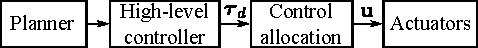
\includegraphics[width=.45\textwidth]{figures/ccta/diagram.pdf}
    \vspace{-1mm}
    \caption{Control system of overactuated vehicles considered in this chapter}
    \label{fig:ccta_diagram}
\end{figure}

\subsection{Notation}
\label{sec:ccta_notation}

Let $\mathbf{p}$ denote the position and $\bs{\Theta}$ the orientation (expressed using the Euler angles) of the vehicle in a \acrfull{ned} reference frame.
%The test models presented in Section~\ref{sec:ccta_simulations} have three degrees of freedom (DOFs), with the position and orientation defined as follows
%\begin{align}
%    \mathbf{p} &= \left[ x ,\, y \right]^{\rm T}, &
%    \bs{\Theta} = \psi,
%\end{align}
%where $x$ is the North coordinate, $y$ is the East coordinate, and $\psi$ is the yaw angle.
%
Let $\pose$ be the pose of the vehicle
\begin{equation}
    \pose = \left[ \mathbf{p}^{\rm T} ,\, \bs{\Theta}^{\rm T} \right]^{\rm T}.
\end{equation}

Let $\vel$ be the velocities of the vehicle in the body-fixed frame.
%For our 3DOF models
%\begin{equation}
%    \vel = \left[ u ,\, v ,\, r \right]^{\rm T},
%\end{equation}
%where $u$ and $v$ are the surge and sway velocities, respectively, and $r$ is the yaw rate.
%
The complete state of the vehicle, $\mathbf{x}$, is defined as
\begin{equation}
    \mathbf{x} = \left[ \pose^{\rm T} \,, \vel^{\rm T} \right]^{\rm T}.
\end{equation}

Let $\bs{\tau}$ be the vector of generalized forces acting on the vehicle.
%For our 3DOF models
%\begin{equation}
%    \bs{\tau} = \left[ X ,\, Y ,\, N \right]^{\rm T},
%\end{equation}
%where $X$ and $Y$ are the forces in the surge and sway direction, respectively, and $N$ is the yaw moment.
Let $K$ be the number of actuator parameters and $\mathbf{u} \in \mathbb{R}^{K}$ the vector of inputs.
Furthermore, let $b : \mathbb{R}^{K} \rightarrow \mathbb{R}^{n_{\rm DOF}}$ be a nonlinear function that maps the inputs to the generalized forces ($n_{\rm DOF}$ is the number of \glspl{dof}).

\subsection{Equations of Motion}

The time-derivative of the pose can be obtained by transforming the velocities. % to the NED frame.
In addition, we assume that the time-derivatives of the velocities are affine in the generalized forces.
We thus consider vehicles described by the following dynamical equations
\begin{equation}
    \dot{\mathbf{x}} = \begin{bmatrix} \dot{\pose} \\ \dot{\vel} \end{bmatrix} = \begin{bmatrix}
        \mathbf{J}(\bs{\Theta})\,\vel \\ f(\mathbf{x}) + g(\mathbf{x})\,\bs{\tau}
    \end{bmatrix} = \begin{bmatrix}
        \mathbf{J}(\bs{\Theta})\,\vel \\ f(\mathbf{x}) + g(\mathbf{x})\,b(\mathbf{u})
    \end{bmatrix},
    \label{eq:ccta_affine_model}
\end{equation}

\noindent where $\mathbf{J}(\bs{\Theta})$ is the transformation matrix. % from body-fixed to NED frame. 
This equation describes a large class of systems, including the matrix-vector model of marine vessels \cite{fossen_handbook_2011}
\begin{subequations}
    \begin{align}
        \dot{\pose} &= \mathbf{J}(\bs{\Theta})\,\vel, \\
        \mathbf{M}\,\dot{\vel} + \left(\mathbf{C}(\vel) + \mathbf{D}(\vel)\right)\,\vel + \mathbf{g}(\pose) &= b(\mathbf{u}),% + \bs{\tau}_w,
    \end{align}
    \label{eq:ccta_matrix_model}
    \vspace{-4mm}
\end{subequations}

\noindent This model can be converted to the form in \eqref{eq:ccta_affine_model} since the matrix $\mathbf{M}$ is invertible.

\da{
\section{Problem Definition}
\label{sec:ccta_problem}

We consider a scenario with $N$ vehicles.
We shall denote the variables that belong to a given vehicle by a lower index (\emph{e.g.,} $\mathbf{x}_{i}$ is the state of the $i^{\rm th}$ vehicle).
Let us assume that each vehicle has access to the position ($\mathbf{p}_i$) and the inertial velocity ($\dot{\mathbf{p}}_i$) of all other vehicles.

Furthermore, let $\boldsymbol{\tau}_{d, i}$ be the desired forces and torques obtained from the high-level controller of vehicle $i$ (see~\figref{fig:ccta_diagram}).
The goal of this chapter is to design a control allocation block that incorporates safety constraints.
This block outputs actuator configuration $\mathbf{u}_i$ that produces the desired forces and torques as closely as possible (\emph{i.e.,} that minimizes the difference between $\boldsymbol{\tau}_{d, i}$ and $b(\mathbf{u}_i)$) while avoiding collisions with other vehicles.
To avoid collisions, we want the vehicle $i$ to satisfy
\begin{align}
    \norm{\mat{p}_i - \mat{p}_j} &\geq d_{\min}, &
    &\forall j \in \{1, \ldots, N\} \setminus \{i\},
\end{align}
where $d_{\min} > 0$ is some minimum safety distance.
}

\section{Control Allocation}
\label{sec:ccta_alloc}

As stated in the Introduction, the goal of the control allocation is to find the inputs that generate the desired forces given by the high-level controller.
For details on control allocation techniques for both linear and nonlinear systems, the reader is referred to \cite{johansen_control_2013}.
\dt{Since control allocation is done individually for each vehicle, we can omit the lower index $i$ in this section.}

In this chapter, we consider systems where the function $b$ can be nonlinear.
In the literature, nonlinear control allocation is commonly solved by linearizing the function $b$ \cite{harkegard_dynamic_2004,johansen_constrained_2004}%, \emph{i.e.,}
\begin{equation}
    b(\mathbf{u}_0 + \Delta\mathbf{u}) \approx b(\mathbf{u}_0) + \mathbf{B}(\mathbf{u}_0)\,\Delta\mathbf{u},
    \label{eq:ccta_forces_approximation}
\end{equation}
where $\mathbf{u}_0$ are the inputs around which we linearize, $\Delta\mathbf{u}$ is the increment, and
\begin{equation}
    \mathbf{B}(\mathbf{u}_0) = \frac{\partial b(\mathbf{u})}{\partial \mathbf{u}}\bigg|_{\mathbf{u}_0},
\end{equation}
is the Jacobian of $b$ evaluated at $\mathbf{u}_0$.
Let $\bs{\tau}_d$ be the desired forces.
The goal of our control allocation scheme is to find optimal inputs $\mathbf{u}^*$ that satisfy
\begin{equation}
    \mathbf{u}^* = \argmin_{\mathbf{u}\in\mathbb{R}^{K}}\,\left\| b(\mathbf{u}) - \bs{\tau}_d \right\|^2.
\end{equation}

Using the approximation \eqref{eq:ccta_forces_approximation}, we can formulate the control allocation problem as a \gls{qp} 
\begin{align}
    \mathbf{u}^* &= \mathbf{u}_0 + \Delta\mathbf{u}^*, \\
    \Delta\mathbf{u}^* &= \argmin_{\Delta\mathbf{u}\in\mathbb{R}^{K}}\,\left\| b(\mathbf{u}_{0}) + \mathbf{B}(\mathbf{u}_{0})\,\Delta\mathbf{u} - \bs{\tau}_{d} \right\|^2.
\end{align} 

\section{Control Barrier Functions}
\label{sec:ccta_CBF}
In this section, we will briefly present the theory behind \acrfullpl{cbf}.
For more details, the reader is referred to \cite{ames_control_2019}.
After presenting the notation for multiple vehicles, we define the \gls{cbf} for \gls{colav}.

\subsection{Introduction to CBFs}
Consider a nonlinear control-affine system
\begin{equation}
    \dot{\mathbf{x}} = \widetilde{f}(\mathbf{x}) + \widetilde{g}(\mathbf{x})\,\mathbf{u},
    \label{eq:ccta_control_affine_system}
\end{equation}
\noindent where $\mathbf{x} \in \mathbb{R}^n$.
Suppose that the system must satisfy a safety constraint
$
    h(\mat{x}) \geq 0,
$
where $h : \mathbb{R}^{n} \rightarrow \mathbb{R}$ is the so-called \emph{barrier function}.
Then, we can define the so-called \emph{safe set}, a set of all states that satisfy the safety constraint, as
\begin{equation}
    \mathcal{C} = \left\{ \mathbf{x} \,|\, h(\mathbf{x}) \geq 0 \right\}.
\end{equation}
If the initial condition of the system \eqref{eq:ccta_control_affine_system} lies in the safe set, the system trajectory will stay within $\mathcal{C}$ if the following inequality holds \cite{ames_control_2019}
\begin{equation}
    \frac{{\rm d}}{{\rm d}t}h(\mathbf{x}) = \frac{\partial h(\mathbf{x})}{\partial \mathbf{x}}\,\left(\widetilde{f}(\mathbf{x}) + \widetilde{g}(\mathbf{x})\,\mathbf{u}\right) \geq - \gamma\bigl(h(\mathbf{x})\bigr),
    \label{eq:ccta_cbf_inequality}
\end{equation}
where $\gamma$ is an extended class-$\mathcal{K}_{\infty}$ function. 
If there exists an input $\mathbf{u}$ such that \eqref{eq:ccta_cbf_inequality} is satisfied, then $h$ is a valid \gls{cbf} for the system \eqref{eq:ccta_control_affine_system}.

\subsection{CBFs for Reactive Collision Avoidance}
%First, we need to extend the notation from Section~\ref{sec:ccta_notation} to multi-vehicle systems.
\dt{Let us define the relative position of vehicles $i$ and $j$ as}
\begin{equation}
    \mathbf{p}_{ij} = \mathbf{p}_{i} - \mathbf{p}_{j}.
    \label{eq:ccta_p_ij}
\end{equation}

To ensure safety, we need a collection of \glspl{cbf} that enforce safe distances between each pair of vehicles.
In the literature, vehicles described by the model \eqref{eq:ccta_affine_model} frequently use \glspl{cbf} in the following form \cite{basso_safety-critical_2020,thyri_reactive_2020}
\begin{equation}
    %h_{ij}(\mathbf{x}_{i}, \mathbf{x}_{j}) = \|\mathbf{p}_{ij}\| - d_{\min} + k_v\,\frac{1}{\|\mathbf{p}_{ij}\|}\,\mathbf{p}_{ij}_{\rm T}\,\dot{\mathbf{p}}_{ij},
    h_{ij}(\mathbf{x}_{i}, \mathbf{x}_{j}) = \|\mathbf{p}_{ij}\| - d_{\min} + k_v\,\frac{\rm d}{{\rm d}t}\|\mathbf{p}_{ij}\|,
    \label{eq:ccta_CBF}
\end{equation}
where $d_{\min}$ is a minimum safe distance, and $k_v$ is a coefficient that penalizes the relative speed of the vehicles.

To use $h_{ij}$ as a control barrier function, we need to calculate its time-derivative.
Differentiating \eqref{eq:ccta_CBF} with respect to time yields
\begin{equation}
    \frac{\rm d}{{\rm d}t}h_{ij}(\mathbf{x}_{i}, \mathbf{x}_{j}) = \frac{\rm d}{{\rm d}t}\|\mathbf{p}_{ij}\| + k_v\,\frac{\rm d^2}{{\rm d}t^2}\|\mathbf{p}_{ij}\|.
\end{equation}

%Note that the norm $\|\mathbf{p}_{ij}\|$ can be defined as
%\begin{equation}
%    \|\mathbf{p}_{ij}\| = \sqrt{(\mathbf{p}_{ij})_{\rm T}\,\mathbf{p}_{ij}}.
%\end{equation}

%By applying the chain rule, we get
%\begin{align}
%    \frac{\rm d}{{\rm d}t}\|\mathbf{p}_{ij}\| &= \frac{1}{\|\mathbf{p}_{ij}\|}\,(\mathbf{p}_{ij})_{\rm T}\,\dot{\mathbf{p}}_{ij}, \\
%    \begin{split}
%        \frac{\rm d_2}{{\rm d}t_2}\|\mathbf{p}_{ij}\| &=  - \frac{1}{\|\mathbf{p}_{ij}\|_3}\,\left((\mathbf{p}_{ij})_{\rm T}\,\dot{\mathbf{p}}_{ij}\right)_2 \\
%        +&\frac{1}{\|\mathbf{p}_{ij}\|}\,\left((\dot{\mathbf{p}}_{ij})_{\rm T}\,\dot{\mathbf{p}}_{ij} + (\mathbf{p}_{ij})_{\rm T}\,\ddot{\mathbf{p}}_{ij}\right).
%    \end{split}        
%\end{align}

To calculate the first and second time-derivative of the relative distance, we need to find the first and second time-derivatives of the relative position.
For $\dot{\mathbf{p}}_{ij}$, we split the derivative of $\pose$ from \eqref{eq:ccta_affine_model} into the derivatives of position and orientation \vspace{-2mm}
\begin{equation}
    \dot{\pose}_{i} = \begin{bmatrix} \dot{\mathbf{p}}_{i} \\ \dot{\bs{\Theta}}_{i} \end{bmatrix} = \begin{bmatrix}
        \mathbf{J}_{\mathbf{p}}(\bs{\Theta}_{i}) \\ \mathbf{J}_{\bs{\Theta}}(\bs{\Theta}_{i})
    \end{bmatrix}\,\vel_{i}.
\end{equation}

\noindent Substituting this into the time-derivative of \eqref{eq:ccta_p_ij} yields
\begin{equation}
    \dot{\mathbf{p}}_{ij} = \mathbf{J}_{\mathbf{p}}(\bs{\Theta}_{i}) \, \vel_{i} - \mathbf{J}_{\mathbf{p}}(\bs{\Theta}_{j}) \, \vel_{j}.
    \label{eq:ccta_p_dot}
\end{equation}

\noindent For $\ddot{\mathbf{p}}_{ij}$, we assume that the \dt{other vehicle} maintains its velocity, \emph{i.e.,}
\begin{equation}
    \ddot{\mathbf{p}}_{ij} \approx \ddot{\mathbf{p}}_{i},
\end{equation}
when calculating the time-derivative for the $i^{\rm th}$ vehicle.
As discussed in \cite{thyri_reactive_2020}, this is a ``mild worst-case'' assumption, since maneuvers of the target vehicle tend to aid to resolving the situation.
Thus, taking the time-derivative of \eqref{eq:ccta_p_dot} yields
\begin{equation}
    \ddot{\mathbf{p}}_{i} = \dot{\mathbf{J}}_{\mathbf{p}}(\bs{\Theta}_{i}) \, \vel_{i} + \mathbf{J}_{\mathbf{p}}(\bs{\Theta}_{i}) \, \dot{\vel}_{i}.
    \label{eq:ccta_p_ddot}
\end{equation}

Finally, we substitute the approximation of forces from \eqref{eq:ccta_forces_approximation} into the equation for $\dot{\vel}$ in \eqref{eq:ccta_affine_model} to get
\begin{equation}
    \dot{\vel}_{i} = f(\mathbf{x}_{i}) + g(\mathbf{x}_{i})\,\left(b(\mathbf{u}_{0,i}) + \mathbf{B}(\mathbf{u}_{0,i})\,\Delta\mathbf{u}_{i}\right),
\end{equation}
which we can substitute into \eqref{eq:ccta_p_ddot} to calculate $\ddot{\mathbf{p}}_{i}$.

\section{Formulating the Optimization Problem}
\label{sec:ccta_optimization}
Now we can combine the definitions from Sections~\ref{sec:ccta_alloc} and \ref{sec:ccta_CBF} to formulate the proposed optimization problem for control allocation with multi-vehicle \gls{colav}.

\subsection{The Basic Optimization Problem}
Let $\mathbf{u}_{0,i}$ be the inputs of vehicle $i$ from the previous control period.
The new inputs are calculated as
\begin{equation}
    \mathbf{u}_{i} = \mathbf{u}_{0,i} + \Delta\mathbf{u}_{i}^*,
\end{equation}
where $\Delta\mathbf{u}_{i}^*$ is obtained by solving the following \gls{qp}
\begin{subequations}
    \begin{align}
        \Delta\mathbf{u}_{i}^* &= \argmin_{\Delta\mathbf{u}_{i}\in\mathbb{R}^{K}}\,\left\| b(\mathbf{u}_{0,i}) + \mathbf{B}(\mathbf{u}_{0,i})\,\Delta\mathbf{u}_{i} - \bs{\tau}_{d,i} \right\|^2\,, \label{eq:ccta_combined_avoidance_allocation_criterion} \\
        \begin{split}
            \text{s.t. }& \frac{{\rm d}}{{\rm d}t}h_{ij}(\mathbf{x}_{i}, \mathbf{x}_{j}) \geq - \gamma\left(h_{ij}(\mathbf{x}_{i}, \mathbf{x}_{j})\right), \\
            & j \in \left\{ 1, \ldots, N \right\} \setminus \left\{ i \right\},
        \end{split} \label{eq:ccta_combined_avoidance_allocation_constraint} \\
        & \mathbf{u}_{i,\min} \leq \mathbf{u}_{0,i} + \Delta\mathbf{u}_{i} \leq \mathbf{u}_{i,\max}, \\
        & \Delta\mathbf{u}_{i,\min} \leq \Delta\mathbf{u}_{i} \leq \Delta\mathbf{u}_{i,\max}, \label{eq:ccta_combined_avoidance_allocation_delta_u}
    \end{align}
    \label{eq:ccta_combined_avoidance_allocation}
\end{subequations}
\noindent where $\mathbf{u}_{i,\min}$ and $\mathbf{u}_{i,\max}$ are the absolute actuator limits, and $\Delta\mathbf{u}_{i,\min}$ and $\Delta\mathbf{u}_{i,\max}$ are the actuator rate limits.
The absolute limits are usually given by the physical limitations of the vehicle (\emph{e.g.,} the thrust of a propeller or the deflection of control surfaces) whereas the rate limits are user-defined to reduce the rapid changes that wear out the actuators.

Simulation results using this control allocation algorithm are presented in Section~\ref{sec:ccta_simulations}.

\subsection{Modified Optimization Problem}
The algorithm in \eqref{eq:ccta_combined_avoidance_allocation} is suitable for vehicles where the number of actuators is equivalent to the number of DOFs.
Applying the algorithm to vehicles where the number of actuators is much greater than the number of DOFs results in inefficient usage of the available actuators, as can be seen in Section~\ref{sec:ccta_simulations}.

To reduce this effect, we add penalty terms on the actuator usage, similar to those proposed in \cite{johansen_constrained_2004}, in the cost function.
To simplify the notation, let $\|\mathbf{x}\|_{\mathbf{Q}}^2$ be the squared norm of a vector $\mathbf{x}$ weighted by a matrix $\mathbf{Q}$, \emph{i.e.,}
\begin{equation}
    \|\mathbf{x}\|_{\mathbf{Q}}^2 = \mathbf{x}^{\rm T}\,\mathbf{Q}\,\mathbf{x}.
\end{equation}

The modified optimization problem is defined as follows
\begin{subequations}
    \begin{align}
    \begin{split}
        \Delta\mathbf{u}_{i}^* &= \argmin_{\Delta\mathbf{u}_{i}\in\mathbb{R}^{K}}\,\left\| b(\mathbf{u}_{i,0}) + \mathbf{B}(\mathbf{u}_{i,0})\,\Delta\mathbf{u}_{i} - \bs{\tau}_{d,i} \right\|_{\mathbf{Q}}^2 \\
        &\quad \quad \quad + \left\| \mathbf{u}_{0,i} + \Delta\mathbf{u}_{i} \right\|_{\mathbf{R}_{\rm abs}}^2 + \left\|\Delta\mathbf{u}_{i}\right\|_{\mathbf{R}_{\rm rel}}^2,
    \end{split} \\    
%    \begin{split}
%        \text{s.t. }& \frac{{\rm d}}{{\rm d}t}h^{ij}(\mathbf{x}^{i}, \mathbf{x}^{j}) \geq - \gamma\left(h^{ij}(\mathbf{x}^{i}, \mathbf{x}^{j})\right), \\
%        & j \in \left\{ 1, \ldots, n \right\} \setminus \left\{ i \right\},
%    \end{split} \\
%    & \mathbf{u}^{i}_{\min} \leq \mathbf{u}^{i}_{0} + \Delta\mathbf{u}^{i} \leq \mathbf{u}^{i}_{\max}, \\
%    & \Delta\mathbf{u}^{i}_{\min} \leq \Delta\mathbf{u}^{i} \leq \Delta\mathbf{u}^{i}_{\max},
    \text{s.t. }&\text{constraints \eqref{eq:ccta_combined_avoidance_allocation_constraint}--\eqref{eq:ccta_combined_avoidance_allocation_delta_u},}
    \end{align}
    \label{eq:ccta_combined_avoidance_allocation_modified}
\end{subequations}
\vspace*{-1em}

\noindent where $\mathbf{Q}$ is a positive definite matrix that penalizes the difference between the desired and actual forces, and $\mathbf{R}_{\rm abs}$ and $\mathbf{R}_{\rm rel}$ are positive semidefinite matrices that penalize the absolute and incremental usage of actuators, respectively.

Note that both \eqref{eq:ccta_combined_avoidance_allocation} and \eqref{eq:ccta_combined_avoidance_allocation_modified} use only local information and measurements, and can thus be solved locally for each vehicle.

When choosing the weight matrices, we first note that the vector $\bs{\tau}$ contains both forces and torques.
The matrix $\mathbf{Q}$ should penalize them differently.
In the simulations in Section~\ref{sec:ccta_simulations}, we choose
\vspace{-1mm}
\begin{equation}
   \mathbf{Q} = \diag{\left(1,1,\frac{1}{L^2}\right)},
   \label{eq:ccta_Q_matrix}
\end{equation}
where $\diag(\cdot)$ is a diagonal matrix and $L$ is the smallest distance of the thrusters from the center of mass.
\da{The matrix $\mathbf{Q}$ is chosen according to \eqref{eq:ccta_Q_matrix} because the term $\boldsymbol{\tau}_{d, i}$ contains both forces and torques.
Specifically, the third element of $\boldsymbol{\tau}_{d, i}$ is the desired yaw torque.
If we divide the squared toruqe error by $L^2$, we effectively convert it to a squared force error.}

\section{Simulations}
\label{sec:ccta_simulations}
In the simulations, we test the ability of the proposed algorithms to resolve a situation when four surface vessels are simultaneously in danger of collision.
Each vessel starts in the corner of a square and is guided towards a reference located in the diagonally opposite corner.

We tested the proposed algorithms on two models of ASVs --- the \emph{milliAmpere} ferry \cite{pedersen_optimization_2019} and the $1:90$ scaled model of the Inocean Cat I drillship \cite{bjorno_thruster-assisted_2016} --- using Simulink.
Both vessels are equipped with azimuth thrusters; the \emph{milliAmpere} has two and the drillship has six.
Each thruster is parametrized by two values: its thrust force and its azimuth.
The input vector for these vessels is defined as \vspace{-1mm}
\begin{equation}
    \mathbf{u} = \left[ f_1 ,\, \ldots ,\, f_k ,\, \alpha_1 ,\, \ldots ,\, \alpha_k \right]^{\rm T},
\end{equation}
where $f_i$ is the thrust force and $\alpha_i$ is the azimuth angle of the $i^{\rm th}$ thruster, and $k$ is the number of thrusters.
%
Both ASV models have 3DOFs, \emph{i.e.,} the North-East position and the yaw angle.
The function that maps the inputs to the generalized forces is \vspace{-1mm}
\begin{equation}
    \scale[0.93]{b(\mathbf{u}) = \sum_{i=1}^k f_i \left[ \cos\alpha_i, \sin\alpha_i, L_x^i\,\sin\alpha_i - L_y^i\,\cos\alpha_i \right]^{\rm T},}
\end{equation}
where $L_x^i$ and $L_y^i$ \da{are the $x$- and $y$-components of} the position of the $i^{\rm th}$ thruster, relative to the center of mass.

\pgfplotsset{table/search path={figures/ccta/data}}
\begin{figure*}[t]
    \centering
    \begin{subfigure}{\linewidth}
        \centering
        %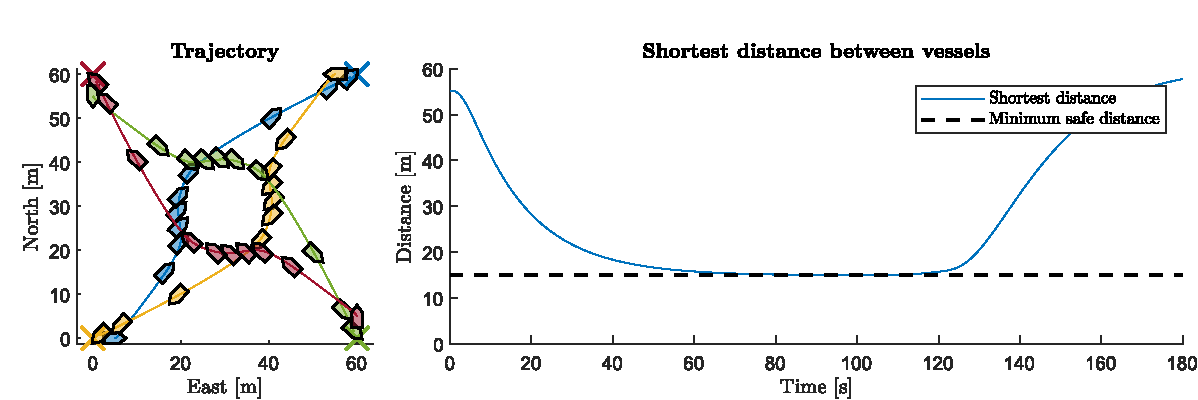
\includegraphics[width = \textwidth]{figures/ccta/milliAmpere_orig.pdf}
        % This file was created by matlab2tikz.
%
%The latest updates can be retrieved from
%  http://www.mathworks.com/matlabcentral/fileexchange/22022-matlab2tikz-matlab2tikz
%where you can also make suggestions and rate matlab2tikz.
%
\definecolor{mycolor1}{rgb}{0.00000,0.44700,0.74100}%
\definecolor{mycolor2}{rgb}{0.85000,0.32500,0.09800}%
\definecolor{mycolor3}{rgb}{0.92900,0.69400,0.12500}%
\definecolor{mycolor4}{rgb}{0.49400,0.18400,0.55600}%

%
\begin{tikzpicture}

\begin{axis}[%
width=0.24\textwidth,
height=0.24\textwidth,
at={(0,0)},
scale only axis,
xmin=-2,
xmax=62,
xlabel style={font=\color{white!15!black}\small, yshift=1.5mm},
xlabel={East [m]},
ticklabel style={font=\small},
ymin=-2,
ymax=62,
ylabel style={font=\color{white!15!black}\small, yshift=-1.5mm},
ylabel={North [m]},
axis background/.style={fill=white},
title style={font=\bfseries, yshift=-2.5mm},
title={Trajectory},
xmajorgrids,
ymajorgrids,
]
\def\nboatplots{7}

\addplot [color=mycolor1, line width=0.8pt]
  table[]{milliAmpere_orig-1.tsv};
\foreach \i in {1,...,\nboatplots}
  \addplot[area legend, draw=black, fill=mycolor1, fill opacity=0.75, line width=0.5pt]
  table[x=x\i, y=y\i]{milliAmpere_orig-asv-1.tsv};

\addplot [color=mycolor2, line width=0.8pt]
  table[]{milliAmpere_orig-2.tsv};
\foreach \i in {1,...,\nboatplots}
  \addplot[area legend, draw=black, fill=mycolor2, fill opacity=0.75, line width=0.5pt]
  table[x=x\i, y=y\i]{milliAmpere_orig-asv-2.tsv};

\addplot [color=mycolor3, line width=0.8pt]
  table[]{milliAmpere_orig-3.tsv};
\foreach \i in {1,...,\nboatplots}
  \addplot[area legend, draw=black, fill=mycolor3, fill opacity=0.75, line width=0.5pt]
  table[x=x\i, y=y\i]{milliAmpere_orig-asv-3.tsv};

\addplot [color=mycolor4, line width=0.8pt]
  table[]{milliAmpere_orig-4.tsv};
\foreach \i in {1,...,\nboatplots}
  \addplot[area legend, draw=black, fill=mycolor4, fill opacity=0.75, line width=0.5pt]
  table[x=x\i, y=y\i]{milliAmpere_orig-asv-4.tsv};

\end{axis}

\begin{axis}[%
width=0.55\textwidth,
height=0.24\textwidth,
at={(0.35\textwidth,0)},
scale only axis,
xmin=0,
xmax=180,
xlabel style={font=\color{white!15!black}\small, yshift=1.5mm},
xlabel={Time [s]},
ymin=0,
ymax=60,
xmajorgrids,
ymajorgrids,
ticklabel style={font=\small},
ylabel style={font=\color{white!15!black}\small, yshift=-1.5mm},
ylabel={Distance [m]},
axis background/.style={fill=white},
title style={font=\bfseries, yshift=-2mm},
title={Shortest distance between vessels},
legend style={/tikz/column 2/.style={column sep=5pt,}, font=\small, at={(0.75,0.95)}, anchor=north east},
]
\addplot [color=mycolor1, line width=0.8pt]
  table[]{milliAmpere_orig-5.tsv};
\addlegendentry{Shortest distance}

\addplot [color=black, dashed, line width=1.5pt]
  table[]{milliAmpere_orig-6.tsv};
\addlegendentry{Minimum distance}

\end{axis}
\end{tikzpicture}%
        \vspace{-0.5em}
        \caption{Algorithm \eqref{eq:ccta_combined_avoidance_allocation} on four \emph{milliAmpere} vessels}
        %\vspace*{1em}
    \end{subfigure}
    \vspace{-1em}
    \begin{subfigure}{\linewidth}
        \centering
        %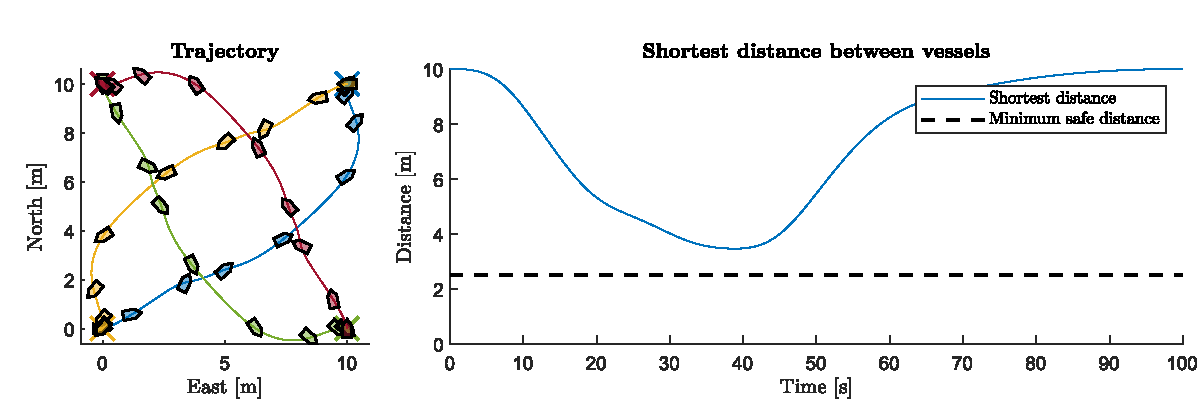
\includegraphics[width = \textwidth]{figures/ccta/drillship_orig.pdf}
        % This file was created by matlab2tikz.
%
%The latest updates can be retrieved from
%  http://www.mathworks.com/matlabcentral/fileexchange/22022-matlab2tikz-matlab2tikz
%where you can also make suggestions and rate matlab2tikz.
%
\definecolor{mycolor1}{rgb}{0.00000,0.44700,0.74100}%
\definecolor{mycolor2}{rgb}{0.85000,0.32500,0.09800}%
\definecolor{mycolor3}{rgb}{0.92900,0.69400,0.12500}%
\definecolor{mycolor4}{rgb}{0.49400,0.18400,0.55600}%

%
\begin{tikzpicture}

\begin{axis}[%
width=0.24\textwidth,
height=0.24\textwidth,
at={(0,0)},
scale only axis,
xmin=-1,
xmax=11,
xlabel style={font=\color{white!15!black}\small, yshift=1.5mm},
xlabel={East [m]},
ticklabel style={font=\small},
ymin=-1,
ymax=11,
ylabel style={font=\color{white!15!black}\small, yshift=-3mm},
ylabel={North [m]},
axis background/.style={fill=white},
title style={font=\bfseries, yshift=-2.5mm},
title={Trajectory},
xmajorgrids,
ymajorgrids,
]
\def\nboatplots{10}

\addplot [color=mycolor1, line width=0.8pt]
  table[]{drillship_orig-1.tsv};
\foreach \i in {1,...,\nboatplots}
  \addplot[area legend, draw=black, fill=mycolor1, fill opacity=0.75, line width=0.5pt]
  table[x=x\i, y=y\i]{drillship_orig-asv-1.tsv};

\addplot [color=mycolor2, line width=0.8pt]
  table[]{drillship_orig-2.tsv};
\foreach \i in {1,...,\nboatplots}
  \addplot[area legend, draw=black, fill=mycolor2, fill opacity=0.75, line width=0.5pt]
  table[x=x\i, y=y\i]{drillship_orig-asv-2.tsv};

\addplot [color=mycolor3, line width=0.8pt]
  table[]{drillship_orig-3.tsv};
\foreach \i in {1,...,\nboatplots}
  \addplot[area legend, draw=black, fill=mycolor3, fill opacity=0.75, line width=0.5pt]
  table[x=x\i, y=y\i]{drillship_orig-asv-3.tsv};

\addplot [color=mycolor4, line width=0.8pt]
  table[]{drillship_orig-4.tsv};
\foreach \i in {1,...,\nboatplots}
  \addplot[area legend, draw=black, fill=mycolor4, fill opacity=0.75, line width=0.5pt]
  table[x=x\i, y=y\i]{drillship_orig-asv-4.tsv};

\end{axis}

\begin{axis}[%
width=0.55\textwidth,
height=0.24\textwidth,
at={(0.35\textwidth,0)},
scale only axis,
xmin=0,
xmax=100,
xlabel style={font=\color{white!15!black}\small, yshift=1.5mm},
xlabel={Time [s]},
ymin=0,
ymax=10,
xmajorgrids,
ymajorgrids,
ticklabel style={font=\small},
ylabel style={font=\color{white!15!black}\small, yshift=-1.75mm},
ylabel={Distance [m]},
axis background/.style={fill=white},
title style={font=\bfseries, yshift=-2mm},
title={Shortest distance between vessels},
legend style={/tikz/column 2/.style={column sep=5pt,}, font=\small, at={(0.99,0.65)}, anchor=north east},
]
\addplot [color=mycolor1, line width=0.8pt]
  table[]{drillship_orig-5.tsv};
%\addlegendentry{Shortest distance}

\addplot [color=black, dashed, line width=1.5pt]
  table[]{drillship_orig-6.tsv};
%\addlegendentry{Minimum distance}

\end{axis}
\end{tikzpicture}%
        \vspace{-2em}
        \caption{Algorithm \eqref{eq:ccta_combined_avoidance_allocation} on four drillships}
    \end{subfigure}
    \caption{Simulations of the control allocation algorithm \eqref{eq:ccta_combined_avoidance_allocation}}
    \label{fig:ccta_orig}
\end{figure*}

\begin{figure}[p]
    \centering
    \begin{subfigure}{\linewidth}
        \centering
        %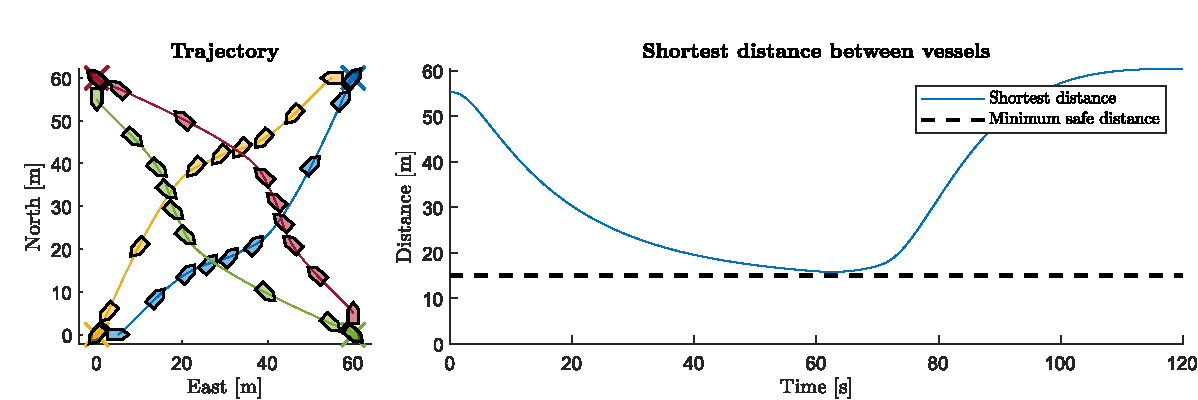
\includegraphics[width = \textwidth]{figures/ccta/milliAmpere_modified.pdf}
        % This file was created by matlab2tikz.
%
%The latest updates can be retrieved from
%  http://www.mathworks.com/matlabcentral/fileexchange/22022-matlab2tikz-matlab2tikz
%where you can also make suggestions and rate matlab2tikz.
%
\definecolor{mycolor1}{rgb}{0.00000,0.44700,0.74100}%
\definecolor{mycolor2}{rgb}{0.85000,0.32500,0.09800}%
\definecolor{mycolor3}{rgb}{0.92900,0.69400,0.12500}%
\definecolor{mycolor4}{rgb}{0.49400,0.18400,0.55600}%

%
\begin{tikzpicture}

\begin{axis}[%
width=0.24\textwidth,
height=0.24\textwidth,
at={(0,0)},
scale only axis,
xmin=-2,
xmax=62,
xlabel style={font=\color{white!15!black}\small, yshift=1.5mm},
xlabel={East [m]},
ticklabel style={font=\small},
ymin=-2,
ymax=62,
ylabel style={font=\color{white!15!black}\small, yshift=-1.5mm},
ylabel={North [m]},
axis background/.style={fill=white},
title style={font=\bfseries, yshift=-2.5mm},
title={Trajectory},
xmajorgrids,
ymajorgrids,
]
\def\nboatplots{10}

\addplot [color=mycolor1, line width=0.8pt]
  table[]{milliAmpere_modified-1.tsv};
\foreach \i in {1,...,\nboatplots}
  \addplot[area legend, draw=black, fill=mycolor1, fill opacity=0.75, line width=0.5pt]
  table[x=x\i, y=y\i]{milliAmpere_modified-asv-1.tsv};

\addplot [color=mycolor2, line width=0.8pt]
  table[]{milliAmpere_modified-2.tsv};
\foreach \i in {1,...,\nboatplots}
  \addplot[area legend, draw=black, fill=mycolor2, fill opacity=0.75, line width=0.5pt]
  table[x=x\i, y=y\i]{milliAmpere_modified-asv-2.tsv};

\addplot [color=mycolor3, line width=0.8pt]
  table[]{milliAmpere_modified-3.tsv};
\foreach \i in {1,...,\nboatplots}
  \addplot[area legend, draw=black, fill=mycolor3, fill opacity=0.75, line width=0.5pt]
  table[x=x\i, y=y\i]{milliAmpere_modified-asv-3.tsv};

\addplot [color=mycolor4, line width=0.8pt]
  table[]{milliAmpere_modified-4.tsv};
\foreach \i in {1,...,\nboatplots}
  \addplot[area legend, draw=black, fill=mycolor4, fill opacity=0.75, line width=0.5pt]
  table[x=x\i, y=y\i]{milliAmpere_modified-asv-4.tsv};

\end{axis}

\begin{axis}[%
width=0.535\textwidth,
height=0.24\textwidth,
at={(0.35\textwidth,0)},
scale only axis,
xmin=0,
xmax=120,
xlabel style={font=\color{white!15!black}\small, yshift=1.5mm},
xlabel={$t$ [s]},
ymin=0,
ymax=60,
xmajorgrids,
ymajorgrids,
ticklabel style={font=\small},
ylabel style={font=\color{white!15!black}\small, yshift=-1.5mm},
ylabel={Distance [m]},
axis background/.style={fill=white},
title style={font=\bfseries, yshift=-2mm},
title={Shortest distance between vessels},
legend style={/tikz/column 2/.style={column sep=5pt,}, font=\small, at={(0.68,0.95)}, anchor=north east},
]
\addplot [color=mycolor1, line width=0.8pt]
  table[]{milliAmpere_modified-5.tsv};
\addlegendentry{Shortest distance}

\addplot [color=black, dashed, line width=1.5pt]
  table[]{milliAmpere_modified-6.tsv};
\addlegendentry{Minimum distance}

\end{axis}
\end{tikzpicture}%
        \caption{Algorithm \eqref{eq:ccta_combined_avoidance_allocation_modified} on four \emph{milliAmpere} vessels}
        \vspace*{1em}
    \end{subfigure}
    \begin{subfigure}{\linewidth}
        \centering
        %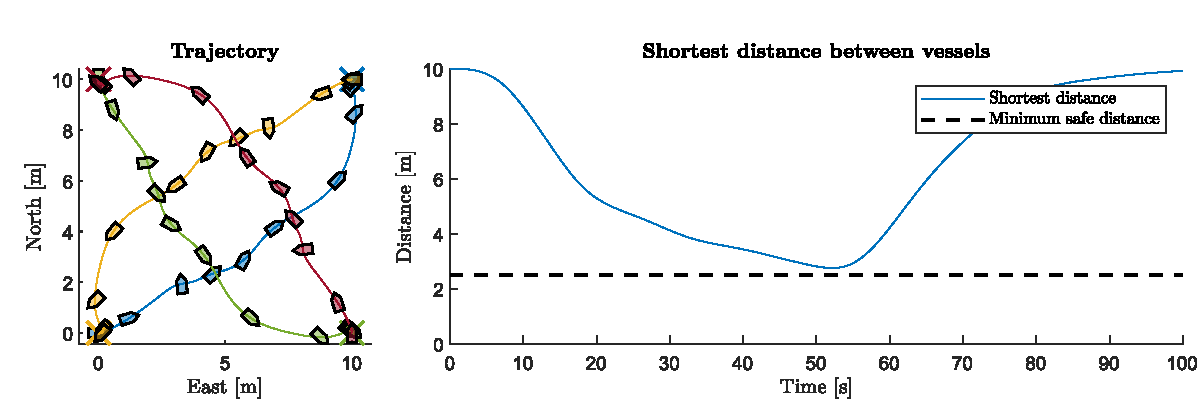
\includegraphics[width = \textwidth]{figures/ccta/drillship_modified.pdf}
        % This file was created by matlab2tikz.
%
%The latest updates can be retrieved from
%  http://www.mathworks.com/matlabcentral/fileexchange/22022-matlab2tikz-matlab2tikz
%where you can also make suggestions and rate matlab2tikz.
%
\definecolor{mycolor1}{rgb}{0.00000,0.44700,0.74100}%
\definecolor{mycolor2}{rgb}{0.85000,0.32500,0.09800}%
\definecolor{mycolor3}{rgb}{0.92900,0.69400,0.12500}%
\definecolor{mycolor4}{rgb}{0.49400,0.18400,0.55600}%

%
\begin{tikzpicture}

\begin{axis}[%
width=0.24\textwidth,
height=0.24\textwidth,
at={(0,0)},
scale only axis,
xmin=-1,
xmax=11,
xlabel style={font=\color{white!15!black}\small, yshift=1.5mm},
xlabel={East [m]},
ticklabel style={font=\small},
ymin=-1,
ymax=11,
ylabel style={font=\color{white!15!black}\small, yshift=-3mm},
ylabel={North [m]},
axis background/.style={fill=white},
title style={font=\bfseries, yshift=-2.5mm},
title={Trajectory},
xmajorgrids,
ymajorgrids,
]
\def\nboatplots{10}

\addplot [color=mycolor1, line width=0.8pt]
  table[]{drillship_modified-1.tsv};
\foreach \i in {1,...,\nboatplots}
  \addplot[area legend, draw=black, fill=mycolor1, fill opacity=0.75, line width=0.5pt]
  table[x=x\i, y=y\i]{drillship_modified-asv-1.tsv};

\addplot [color=mycolor2, line width=0.8pt]
  table[]{drillship_modified-2.tsv};
\foreach \i in {1,...,\nboatplots}
  \addplot[area legend, draw=black, fill=mycolor2, fill opacity=0.75, line width=0.5pt]
  table[x=x\i, y=y\i]{drillship_modified-asv-2.tsv};

\addplot [color=mycolor3, line width=0.8pt]
  table[]{drillship_modified-3.tsv};
\foreach \i in {1,...,\nboatplots}
  \addplot[area legend, draw=black, fill=mycolor3, fill opacity=0.75, line width=0.5pt]
  table[x=x\i, y=y\i]{drillship_modified-asv-3.tsv};

\addplot [color=mycolor4, line width=0.8pt]
  table[]{drillship_modified-4.tsv};
\foreach \i in {1,...,\nboatplots}
  \addplot[area legend, draw=black, fill=mycolor4, fill opacity=0.75, line width=0.5pt]
  table[x=x\i, y=y\i]{drillship_modified-asv-4.tsv};

\end{axis}

\begin{axis}[%
width=0.55\textwidth,
height=0.24\textwidth,
at={(0.35\textwidth,0)},
scale only axis,
xmin=0,
xmax=100,
xlabel style={font=\color{white!15!black}\small, yshift=1.5mm},
xlabel={$t$ [s]},
ymin=0,
ymax=10,
xmajorgrids,
ymajorgrids,
ticklabel style={font=\small},
ylabel style={font=\color{white!15!black}\small, yshift=-1.75mm},
ylabel={Distance [m]},
axis background/.style={fill=white},
title style={font=\bfseries, yshift=-2mm},
title={Shortest distance between vessels},
legend style={/tikz/column 2/.style={column sep=5pt,}, font=\small, at={(0.99,0.65)}, anchor=north east},
]
\addplot [color=mycolor1, line width=0.8pt]
  table[]{drillship_modified-5.tsv};
%\addlegendentry{Shortest distance}

\addplot [color=black, dashed, line width=1.5pt]
  table[]{drillship_modified-6.tsv};
%\addlegendentry{Minimum distance}

\end{axis}
\end{tikzpicture}%
        \caption{Algorithm \eqref{eq:ccta_combined_avoidance_allocation_modified} on four drillships}
    \end{subfigure}
    \caption{Simulations of the modified control allocation algorithm \eqref{eq:ccta_combined_avoidance_allocation_modified}}
    \label{fig:ccta_modified}
\end{figure}

\begin{table}[p]
    \centering
    \begin{tabular}{c|cc}
        {\bf Parameter} & {\bf \emph{milliAmpere}} & {\bf drillship} \\ \hline
        %$\bs{\Omega}_{bw}$ & $\diag{(0.1,\,0.1,\,0.5)}$ & $\diag{(0.1,\,0.1,\,0.5)}$ \\
        $\bs{\Omega}_{bw}$ & \multicolumn{2}{c}{$\diag{(0.1,\,0.1,\,0.5)}$} \\
        %$\mathbf{Z}$ & $\diag{(0.95,\,0.95,\,0.97)}$ & $\diag{(0.95,\,0.95,\,0.97)}$ \\
        $\mathbf{Z}$ & \multicolumn{2}{c}{$\diag{(0.95,\,0.95,\,0.97)}$} \\
        $\mathbf{Q}$ & $\diag{(1,1,0.7)}$ & $\diag{(1,1,1.13)}$ \\
        %$\mathbf{R}_{\rm abs}$ & $\begin{bmatrix} \mathbf{I}_{2 \times 2} & \\ & \mathbf{0}_{2 \times 2} \end{bmatrix}$ & $\begin{bmatrix} \mathbf{I}_{6 \times 6} & \\ & \mathbf{0}_{6 \times 6} \end{bmatrix}$ \\
        $r_{\rm abs}$ & $1$ & $1$ \\
        %$\mathbf{R}_{\rm rel}$ & $\begin{bmatrix} \mathbf{0}_{2 \times 2} & \\ & 100\mathbf{I}_{2 \times 2} \end{bmatrix}$ & $\begin{bmatrix} \mathbf{0}_{6 \times 6} & \\ & \mathbf{I}_{6 \times 6} \end{bmatrix}$ \\
        $r_{\rm rel}$ & $100$ & $1$ \\
        $d_{\min} \, [{\rm m}]$ & $15$ & $2.5$ \\
        $k_v \, [{\rm s}]$ & $15$ & $15$ \\
        $\gamma(h)$ & $0.1\,h$ & $0.1\,h$ \\
        $f_{\min} \, [{\rm N}]$ & $-350$ & $-0.8$ \\
        $f_{\max} \, [{\rm N}]$ & $500$ & $1.5$ \\
        $\Delta f_{\max} \, [{\rm N}]$ & $350$ & $0.5$ \\
        $\Delta \alpha_{\max} \, [{\rm rad}]$ & $\frac{\pi}{8}$ & $\frac{\pi}{8}$
    \end{tabular}
    \caption{Simulation parameters. Parameters $\bs{\Omega}_{bw}$ and $\bs{Z}$ are identical for both scenarios, $\diag{(.)}$ is a diagonal matrix}
    \label{tab:ccta_params}
\end{table}

For the higher-level controller that provides the desired forces, we use a nonlinear PID controller \cite{fossen_handbook_2011}.
The nonlinear PID is an output-linearizing controller that transforms the nonlinear dynamical equations from \eqref{eq:ccta_matrix_model} to
\vspace{-1mm}
\begin{equation}
    \ddot{\pose} + 2\,\bs{\Omega}_n\,\mathbf{Z}\,\dot{\pose} + \bs{\Omega}_n^2\,\pose = 0,
\end{equation}
where $\mathbf{Z}$ is the diagonal relative damping matrix, and $\bs{\Omega}_n$ is the diagonal natural frequency matrix.
Both matrices are tuning parameters.
For convenience, we express $\bs{\Omega}_n$ in terms of a bandwidth matrix $\bs{\Omega}_{bw}$
\vspace{-1mm}
\begin{equation}
    \bs{\Omega}_n = \bs{\Omega}_{bw} \, \left(\sqrt{\mathbf{I} - 2\,\mathbf{Z}^2 + \sqrt{4\,\mathbf{Z}^4 - 4\,\mathbf{Z}^2 + 2\,\mathbf{I}}}\right)^{-1},
\end{equation}
where $\sqrt{.}$ is an elementwise square root.

The simulation parameters for both vessels are summarized in Table~\ref{tab:ccta_params}.
% The matrix $\mathbf{Q}$ is chosen as
% \begin{align}
%     \mathbf{Q} &= \diag{\left( 1,1,\frac{1}{L^2} \right)},&
%     L &= \min_{i} \sqrt{\left(L_x^i\right)^2 + \left(L_y^i\right)^2}.
% \end{align}

\noindent Since the power consumption of a thruster increases with the absolute value of its thrust force and the increment of its azimuth, the matrices $\mathbf{R}_{\rm abs}$ and $\mathbf{R}_{\rm rel}$ are chosen as
%\begin{align}
%    \mathbf{R}_{\rm abs} &= \begin{bmatrix} r_{\rm abs}\,\mathbf{I}_{k} & \\ & \mathbf{0}_{k \times k} \end{bmatrix},
%    \mathbf{R}_{\rm rel} &= \begin{bmatrix} \mathbf{0}_{k \times k} & \\ & r_{\rm rel}\,\mathbf{I}_{k} \end{bmatrix},
%\end{align}
\begin{equation}
    \scale[0.931]{\mathbf{R}_{\rm abs} = \begin{bmatrix} r_{\rm abs}\,\mathbf{I}_{k} & \mathbf{O}_{k \times k} \\ \mathbf{O}_{k \times k} & \mathbf{O}_{k \times k} \end{bmatrix}, \,
    \mathbf{R}_{\rm rel} = \begin{bmatrix} \mathbf{O}_{k \times k} & \mathbf{O}_{k \times k} \\ \mathbf{O}_{k \times k} & r_{\rm rel}\,\mathbf{I}_{k} \end{bmatrix},}
\end{equation}
The rate constraints are identical for all thrusters and symmetric, \emph{i.e.,}
\begin{align}
    \Delta\mathbf{u}_{\max} &= \begin{bmatrix} \Delta f_{\max}\,\mathbf{1}_k \\ \Delta \alpha_{\max}\,\mathbf{1}_k \end{bmatrix}, &
    \Delta\mathbf{u}_{\min} &= - \Delta\mathbf{u}_{\max},
\end{align}
where $\Delta f_{\max}$ and $\Delta \alpha_{\max}$ are the force and azimuth rate constraints, respectively, and $\mathbf{1}_k$ is a vector of ones.

\begin{figure}[t]
    \centering
    \begin{subfigure}{\linewidth}
        \centering
        %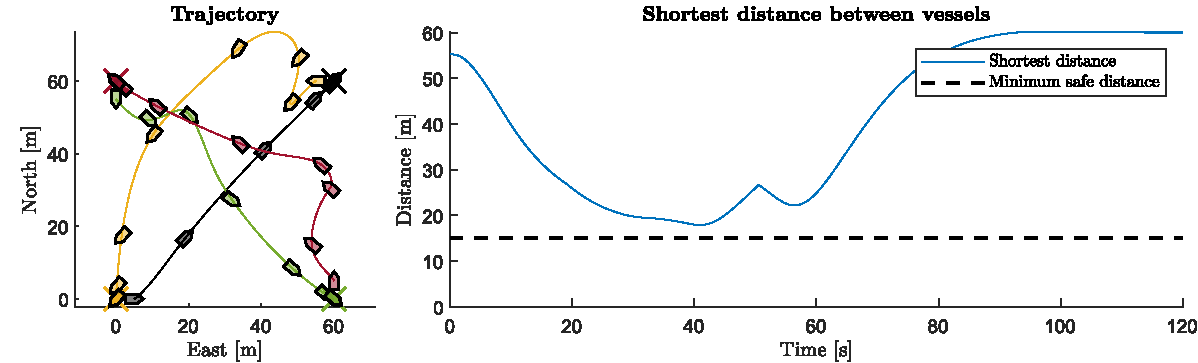
\includegraphics[width = \textwidth]{figures/ccta/milliAmpere_modified_uncontrolled.pdf}
        % This file was created by matlab2tikz.
%
%The latest updates can be retrieved from
%  http://www.mathworks.com/matlabcentral/fileexchange/22022-matlab2tikz-matlab2tikz
%where you can also make suggestions and rate matlab2tikz.
%
\definecolor{mycolor1}{rgb}{0.00000,0.44700,0.74100}%
\definecolor{mycolor2}{rgb}{0.85000,0.32500,0.09800}%
\definecolor{mycolor3}{rgb}{0.92900,0.69400,0.12500}%
\definecolor{mycolor4}{rgb}{0.49400,0.18400,0.55600}%

%
\begin{tikzpicture}

\begin{axis}[%
width=0.24\textwidth,
height=0.24\textwidth,
at={(0,0)},
scale only axis,
xmin=-10,
xmax=70,
xlabel style={font=\color{white!15!black}\small, yshift=1.5mm},
xlabel={East [m]},
ticklabel style={font=\small},
ymin=-4,
ymax=78,
ylabel style={font=\color{white!15!black}\small, yshift=-1.5mm},
ylabel={North [m]},
axis background/.style={fill=white},
title style={font=\bfseries, yshift=-2.5mm},
title={Trajectory},
xmajorgrids,
ymajorgrids,
]
\def\nboatplots{10}

\addplot [color=black, line width=0.8pt]
  table[]{milliAmpere_modified_uncontrolled-1.tsv};
\foreach \i in {1,...,\nboatplots}
  \addplot[area legend, draw=black, fill=black, fill opacity=0.75, line width=0.5pt]
  table[x=x\i, y=y\i]{milliAmpere_modified_uncontrolled-asv-1.tsv};

\addplot [color=mycolor2, line width=0.8pt]
  table[]{milliAmpere_modified_uncontrolled-2.tsv};
\foreach \i in {1,...,\nboatplots}
  \addplot[area legend, draw=black, fill=mycolor2, fill opacity=0.75, line width=0.5pt]
  table[x=x\i, y=y\i]{milliAmpere_modified_uncontrolled-asv-2.tsv};

\addplot [color=mycolor3, line width=0.8pt]
  table[]{milliAmpere_modified_uncontrolled-3.tsv};
\foreach \i in {1,...,\nboatplots}
  \addplot[area legend, draw=black, fill=mycolor3, fill opacity=0.75, line width=0.5pt]
  table[x=x\i, y=y\i]{milliAmpere_modified_uncontrolled-asv-3.tsv};

\addplot [color=mycolor4, line width=0.8pt]
  table[]{milliAmpere_modified_uncontrolled-4.tsv};
\foreach \i in {1,...,\nboatplots}
  \addplot[area legend, draw=black, fill=mycolor4, fill opacity=0.75, line width=0.5pt]
  table[x=x\i, y=y\i]{milliAmpere_modified_uncontrolled-asv-4.tsv};

\end{axis}

\begin{axis}[%
width=0.54\textwidth,
height=0.24\textwidth,
at={(0.35\textwidth,0)},
scale only axis,
xmin=0,
xmax=120,
xlabel style={font=\color{white!15!black}\small, yshift=1.5mm},
xlabel={Time [s]},
ymin=0,
ymax=61,
xmajorgrids,
ymajorgrids,
ticklabel style={font=\small},
ylabel style={font=\color{white!15!black}\small, yshift=-1.5mm},
ylabel={Distance [m]},
axis background/.style={fill=white},
title style={font=\bfseries, yshift=-2mm},
title={Shortest distance between vessels},
legend style={/tikz/column 2/.style={column sep=5pt,}, font=\small, at={(0.675,0.95)}, anchor=north east},
]
\addplot [color=mycolor1, line width=0.8pt]
  table[]{milliAmpere_modified_uncontrolled-5.tsv};
%\addlegendentry{Shortest distance}

\addplot [color=black, dashed, line width=1.5pt]
  table[]{milliAmpere_modified_uncontrolled-6.tsv};
%\addlegendentry{Minimum distance}

\end{axis}
\end{tikzpicture}%
        \vspace{-6mm}
        \caption{Algorithm \eqref{eq:ccta_combined_avoidance_allocation_modified} on four \emph{milliAmpere} vessels with one uncontrolled vessel}
        \vspace{0em}
    \end{subfigure}
    \begin{subfigure}{\linewidth}
        \centering
        %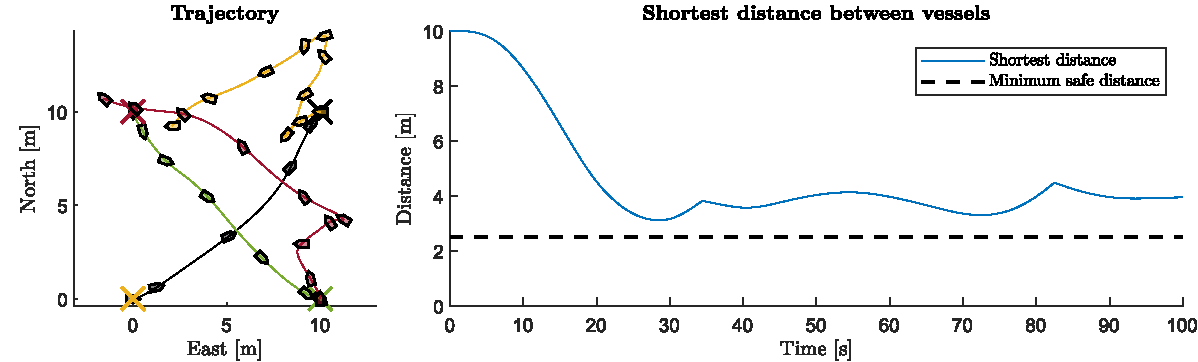
\includegraphics[width = \textwidth]{figures/ccta/drillship_modified_uncontrolled.pdf}
        % This file was created by matlab2tikz.
%
%The latest updates can be retrieved from
%  http://www.mathworks.com/matlabcentral/fileexchange/22022-matlab2tikz-matlab2tikz
%where you can also make suggestions and rate matlab2tikz.
%
\definecolor{mycolor1}{rgb}{0.00000,0.44700,0.74100}%
\definecolor{mycolor2}{rgb}{0.85000,0.32500,0.09800}%
\definecolor{mycolor3}{rgb}{0.92900,0.69400,0.12500}%
\definecolor{mycolor4}{rgb}{0.49400,0.18400,0.55600}%

%
\begin{tikzpicture}

\begin{axis}[%
width=0.24\textwidth,
height=0.24\textwidth,
at={(0,0)},
scale only axis,
xmin=-3,
xmax=13,
xlabel style={font=\color{white!15!black}\small, yshift=1.5mm},
xlabel={East [m]},
ticklabel style={font=\small},
ymin=-1,
ymax=15,
ylabel style={font=\color{white!15!black}\small, yshift=-3mm},
ylabel={North [m]},
axis background/.style={fill=white},
title style={font=\bfseries, yshift=-2.5mm},
title={Trajectory},
xmajorgrids,
ymajorgrids,
]
\def\nboatplots{10}

\addplot [color=black, line width=0.8pt]
  table[]{drillship_modified_uncontrolled-1.tsv};
\foreach \i in {1,...,\nboatplots}
  \addplot[area legend, draw=black, fill=black, fill opacity=0.75, line width=0.5pt]
  table[x=x\i, y=y\i]{drillship_modified_uncontrolled-asv-1.tsv};

\addplot [color=mycolor2, line width=0.8pt]
  table[]{drillship_modified_uncontrolled-2.tsv};
\foreach \i in {1,...,\nboatplots}
  \addplot[area legend, draw=black, fill=mycolor2, fill opacity=0.75, line width=0.5pt]
  table[x=x\i, y=y\i]{drillship_modified_uncontrolled-asv-2.tsv};

\addplot [color=mycolor3, line width=0.8pt]
  table[]{drillship_modified_uncontrolled-3.tsv};
\foreach \i in {1,...,\nboatplots}
  \addplot[area legend, draw=black, fill=mycolor3, fill opacity=0.75, line width=0.5pt]
  table[x=x\i, y=y\i]{drillship_modified_uncontrolled-asv-3.tsv};

\addplot [color=mycolor4, line width=0.8pt]
  table[]{drillship_modified_uncontrolled-4.tsv};
\foreach \i in {1,...,\nboatplots}
  \addplot[area legend, draw=black, fill=mycolor4, fill opacity=0.75, line width=0.5pt]
  table[x=x\i, y=y\i]{drillship_modified_uncontrolled-asv-4.tsv};

\end{axis}

\begin{axis}[%
width=0.55\textwidth,
height=0.24\textwidth,
at={(0.35\textwidth,0)},
scale only axis,
xmin=0,
xmax=100,
xlabel style={font=\color{white!15!black}\small, yshift=1.5mm},
xlabel={$t$ [s]},
ymin=0,
ymax=10.1,
xmajorgrids,
ymajorgrids,
ticklabel style={font=\small},
ylabel style={font=\color{white!15!black}\small, yshift=-1.75mm},
ylabel={Distance [m]},
axis background/.style={fill=white},
title style={font=\bfseries, yshift=-2mm},
title={Shortest distance between vessels},
legend style={/tikz/column 2/.style={column sep=5pt,}, font=\small, at={(0.98,0.97)}, anchor=north east},
]
\addplot [color=mycolor1, line width=0.8pt]
  table[]{drillship_modified_uncontrolled-5.tsv};
\addlegendentry{Shortest distance}

\addplot [color=black, dashed, line width=1.5pt]
  table[]{drillship_modified_uncontrolled-6.tsv};
\addlegendentry{Minimum distance}

\end{axis}
\end{tikzpicture}%
        \vspace{-6mm}
        \caption{Algorithm \eqref{eq:ccta_combined_avoidance_allocation_modified} on four drillships with one uncontrolled vessel}
        \label{fig:ccta_drillship_unc}
        \vspace{-1.5mm}
    \end{subfigure}
    \caption{Simulations of the modified control allocation algorithm \eqref{eq:ccta_combined_avoidance_allocation_modified} with one uncontrolled vessel (plotted in black)}
    \label{fig:ccta_uncontrolled}
\end{figure}

The results of the simulations are shown in Figures \ref{fig:ccta_orig}, \ref{fig:ccta_modified}, and \ref{fig:ccta_uncontrolled}.
Figure \ref{fig:ccta_orig} shows the results of algorithm \eqref{eq:ccta_combined_avoidance_allocation}.
Figure \ref{fig:ccta_modified} shows the results of algorithm \eqref{eq:ccta_combined_avoidance_allocation_modified}.
Each figure consists of two plots.
The plot on the left displays the trajectory of the vessels.
The colored lines show the trajectory of each vessel, the boat-shaped polygons represent the pose of the vessels at several evenly spaced time-instances, and the colored crosses show the reference of each vessel.
The plot on the right shows the smallest distance between the vessels compared to the minimum safe distance $d_{\min}$.
In both scenarios, the vessels reach their reference position while maintaining safe distance.

We also tested a scenario where one of the vessels is uncontrolled.
The results are shown in Figure~\ref{fig:ccta_uncontrolled}.
In this scenario, the uncontrolled vessel (plotted in black) solves the control allocation problem without the \gls{cbf} constraints \eqref{eq:ccta_combined_avoidance_allocation_constraint}.
Although the time it takes the vessels to converge to their goal positions is greater, the minimum safe distance is still maintained.
\dt{Note that in \figref{fig:ccta_drillship_unc}, the red vessel does not seem to converge to its desired position.
This is because the simulation was terminated too early, after 100 seconds.
Given more time, the vessel would eventually converge to its desired position.}

In this section, we have provided some insight into how to chose some of the parameters for the simulated models.
When it comes to the choice of the coefficient $k_v$, introduced in \eqref{eq:ccta_CBF}, and the extended class-$\mathcal{K}_{\infty}$ function $\gamma$, introduced in \eqref{eq:ccta_combined_avoidance_allocation}, the following considerations can be made.
Intuitively, increasing $k_v$ increases the size of the ``unsafe'' region where the barrier function is negative, causing the system to react sooner in situations where two vehicles are on collision course.
Conversely, increasing the slope of $\gamma$ decreases the size of the region where the constraint \eqref{eq:ccta_combined_avoidance_allocation_constraint} is active, causing the system to react later.

\begin{table}[t]
    \centering
    \begin{tabular}{cc|rrr}
        \multirow{2}{*}{\textbf{Vessel}} & \multirow{2}{*}{\textbf{Scenario}} & \multicolumn{3}{|c}{\textbf{Thruster utilization [\%]}} \\
        & & \textbf{Maximum} & \textbf{Minimum} & \textbf{Mean} \\ \hline
        \multirow{2}{*}{\textbf{milliAmpere}} & \textbf{basic} & $2.074$ & $1.550$ & $1.822$ \\
        & \textbf{modified} & $0.838$ & $0.835$ & $0.837$ \\
        \multirow{2}{*}{\textbf{drillship}} & \textbf{basic} & $100.000$ & $1.282$ & $51.496$ \\
        & \textbf{modified} & $6.161$ & $0.259$ & $3.816$ 
    \end{tabular}
    \caption{Steady-state thruster utilization of the \emph{basic} algorithm \eqref{eq:ccta_combined_avoidance_allocation} and the \emph{modified} algorithm \eqref{eq:ccta_combined_avoidance_allocation_modified}.}
    \label{tab:thruster_utilization}
\end{table}

\part{Formation Path-following using the Null-space-based Behavioral Algorithm}
\label{part:NSB}

\chapter{Formation Path-following Control of 5DOF Underactuated AUVs}
\label{chap:5dof_nsb}

\setlength{\epigraphwidth}{0.55\textwidth}
\epigraph{\it
    An ant is very stupid \dots \\ and yet, many ants together are smart.
}{
    Kurzgesagt --- In a Nutshell, ``Emergence,'' \url{youtu.be/16W7c0mb-rE}.
}

This chapter presents a novel method for formation path following of multiple underactuated autonomous underwater vehicles.
The method combines \acrlong{los} guidance with \acrlong{nsb} control, allowing the vehicles to follow curved paths while maintaining the desired formation.
We investigate the dynamics of the path-following error using cascaded systems theory, and show that the closed-loop system is \acrlongpl{usges}.
We validate the theoretical results through numerical simulations.
The contents of this chapter are based on \cite{matouvs_formation_2022}.

\section{Introduction}

The work presented in this chapter extends the results of \cite{eek_formation_2021}, where a \acrfull{nsb} algorithm is used to guide two surface vessels moving in the horizontal plane.
Specifically, we propose an algorithm that works with an arbitrary number of \acrfullpl{auv} with five \acrfullpl{dof} moving in 3D.
Similarly to \cite{eek_formation_2021}, we solve the path-following task using \acrfull{los} guidance.
Using the cascaded systems theory results of \cite{pettersen_lyapunov_2017}, we prove that the closed-loop system consisting of a decoupled \gls{los} guidance law, combined with surge, pitch, and yaw autopilots based on \cite{moe_LOS_2016}, is \acrfullpl{usges} and \acrfullpl{ugas}.
The theoretical results are verified through numerical simulations.

The remainder of the chapter is organized as follows.
Section \ref{sec:nsb_5dof_model} defines the formation path-following problem that is addressed in this chapter.
In Section \ref{sec:nsb_5dof_control}, we describe the control system.
The stability of the control system is proven in Section \ref{sec:nsb_5dof_path_stability}.
Section \ref{sec:nsb_5dof_simulations} contains the results of a numerical simulation.
Finally, Section \ref{sec:nsb_5dof_conclusion} contains some concluding remarks.

\section{Problem Definition}
\label{sec:nsb_5dof_model}
In this section, we briefly present the \gls{auv} model and the formation path-following problem.

\subsection{Vehicle Model}
We consider a fleet of $N$ underactuated \glspl{auv}.
The dynamics are described using the 5\gls{dof} control-oriented model from Section~\ref{sec:model_control_oriented}.
The pose ($\pose_i$) and velocities ($\vel_i$) of the $i^{\rm th}$ \gls{auv} are defined as
\begin{align}
    \pose_i &= \left[x_i, y_i, z_i, \theta_i, \psi_i\right]\T, &
    \vel_i &= \left[u_i, v_i, w_i, q_i, r_i\right]\T.
\end{align}
The roll dynamics are disregarded as the roll motion is assumed to be small and self-stabilizing by the vehicle design.
Let $\ocean \in \mathbb{R}^3$ be the velocity of an unknown, constant and irrotational ocean current.

Recalling \eqref{eq:background_component_form_5DOF}, the dynamics of the $i^{\rm th}$ \gls{auv} are
\begin{subequations}
    \begin{align}
        \scale[0.93]{\dot{x}} &= \scale[0.93]{u\,\cos\left(\psi \right)\,\cos\left(\theta \right)-v\,\sin\left(\psi \right)+w\,\cos\left(\psi \right)\,\sin\left(\theta \right),} \\
        \scale[0.93]{\dot{y}} &= \scale[0.93]{u\,\cos\left(\theta \right)\,\sin\left(\psi \right)+v\,\cos\left(\psi \right)+w\,\sin\left(\psi \right)\,\sin\left(\theta \right),} \\
        \scale[0.93]{\dot{z}} &= \scale[0.93]{-u\,\sin\left(\theta \right)+w\,\cos\left(\theta \right),} \\
        \scale[0.93]{\dot{\theta}} &= \scale[0.93]{q,} \label{eq:nsb_5dof_theta_dot} \\
        \scale[0.93]{\dot{\psi}} &= \scale[0.93]{\frac{1}{\cos\left(\theta \right)}\,r,} \label{eq:nsb_5dof_psi_dot} \\
        \scale[0.93]{\dot{u}} &= \scale[0.93]{f_u + F_u(u, v, w, q, r) + \bs{\phi}_u(u, v, w, q, r, \theta, \psi)\T\,\ocean,} \label{eq:nsb_5dof_u_dot} \\
        \scale[0.93]{\dot{v}} &= \scale[0.93]{X_v(u, u_c)\,r + Y_v(u, u_c)\,v_r,} \\
        \scale[0.93]{\dot{w}} &= \scale[0.93]{X_w(u, u_c)\,q + Y_w(u, u_c)\,w_r + G(\theta),} \\
        \scale[0.93]{\dot{q}} &= \scale[0.93]{t_q + F_q(u, w, q, \theta) + \bs{\phi}_q(u, w, q, \theta, \psi)\T\,\mathbb{V}_c,} \label{eq:nsb_5dof_q_dot} \\
        \scale[0.93]{\dot{r}} &= \scale[0.93]{t_r + F_r(u, v, r) + \bs{\phi}_r(u, v, r, \theta, \psi)\T\,\mathbb{V}_c.} \label{eq:nsb_5dof_r_dot} 
    \end{align} \label{eq:nsb_5dof_components}
\end{subequations}

\subsection{Control Objectives}
\label{sec:nsb_5dof_objectives}
The goal is to control the \glspl{auv} so that they move in a prescribed formation while avoiding collisions, and their barycenter follows a given path.

The prescribed path is parametrized by a smooth function $\mat{p}_p: \mathbb{R} \rightarrow \mathbb{R}^3$.
We assume that the parametrization is $\mathcal{C}^2$ and regular.
Therefore, for every point $\mat{p}_p(s)$ on the path, there exist path-tangential angles, $\theta_p(s)$ and $\psi_p(s)$, and a corresponding path-tangential coordinate frame (see Section~\ref{sec:background_paths} for more details).

The path-following error $\mat{p}_b^p$ is given by the position of the barycenter expressed in the path-tangential coordinate frame
\begin{equation}
    \mat{p}_b^p = \mat{R}_p(s)\T \, \big(\mat{p}_b - \mat{p}_p(s)\big), \label{eq:nsb_5dof_barycenter}
\end{equation}
where
\begin{align}
    \mat{p}_b &= \frac{1}{n} \sum_{i=1}^n \mat{p}_i, & 
    \mat{p}_i &= \left[x_i, y_i, z_i\right]\T.
\end{align}

The vehicles should converge to a dynamic formation that rotates with the desired path (see Section~\ref{sec:background_formation_keeping} for details).
Let $\mat{p}_{f,1}^f, \ldots, \mat{p}_{f,n}^f$ be the position vectors that represent the desired formation.
The objective is to control the vehicles so that
\begin{align}
    \mat{p}_i - \mat{p}_b &\rightarrow \mat{R}_p(s) \mat{p}_{f,i}^f + \mat{p}_b, &
    i &\in \left\{1, \ldots, n \right\}.
\end{align}

\section{Control System}
\label{sec:nsb_5dof_control}
To solve the formation path following problem, we propose a method that combines \acrfull{colav}, formation keeping, and path following in a hierarchic manner using an \gls{nsb} algorithm.
Since the \gls{nsb} algorithm outputs inertial velocity references, we also need a low-level attitude control system to track these references.

In this section, we first present the attitude control system.
Then, in Section~\ref{sec:nsb_5dof_NSB}, we present the \gls{nsb} algorithm and the associated tasks.
Finally, in Section~\ref{sec:nsb_5dof_path_parameter}, we demonstrate how to use the update law of the path variable to cancel unwanted terms in the path-following error dynamics.

\subsection{Attitude Control System}
\label{sec:nsb_5dof_ACS}
This system controls the surge velocity, pitch, and yaw via the corresponding accelerations.
The system is based on the autopilots in \cite{moe_LOS_2016}, but extended to five \glspl{dof}.

Let $u_d$ be the desired surge velocity and $\dot{u}_d$ its derivative.
Let $\oceanhat$ be the estimate of the ocean current.
Furthermore, let us define $\tilde{u} = u - u_d$ and $\oceantilde = \oceanhat - \ocean$.
The surge controller consists of an output-linearizing sliding-mode P-controller and an ocean current observer \vspace{-1mm}
\begin{align}
    f_u &= \dot{u}_d - F_u(\cdot) - \bs{\phi}_u(\cdot)\T\,\oceanhat - k_u\,\tilde{u} - k_c\,{\rm sign}\left(\tilde{u}\right), \label{eq:nsb_5dof_t_u} \\
    \dot{\hat{\ivel}}_c &= c_u\,\bs{\phi}_u(\cdot)\,\tilde{u}, \label{eq:nsb_5dof_V_hat_u} \vspace{-2mm}
\end{align}
where $k_u$, $k_c$ and $c_u$ are positive gains.

Let $\theta_d$ be the desired pitch angle and $\dot{\theta}_d, \ddot{\theta}_d$ its derivatives.
Let $\hat{\mathbb{V}}_q$ be the estimate of $\mathbb{V}_c$.
Furthermore, let us define $\tilde{\theta} = \theta - \theta_d$, $\tilde{q} = q - \dot{\theta}_d$ and $\tilde{\mathbb{V}}_q = \hat{\mathbb{V}}_q - \mathbb{V}_c$.
Inspired by \cite{moe_set-based_2017}, we introduce the following transformation \vspace{-1.5mm}
\begin{equation}
    s_q = \tilde{q} + \lambda_q\,\tilde{\theta}, \vspace{-2mm}
\end{equation}
where $\lambda_q$ is a positive constant.
The pitch controller consists of an output-linearizing sliding-mode PD-controller and an ocean current observer \vspace{-1mm}
\begin{align}
    \begin{split}
        t_q &= \ddot{\theta}_d - F_q(\cdot) - \bs{\phi}_q(\cdot)\T\,\hat{\mathbb{V}}_q - \lambda_q\,\tilde{q} \\
        & \quad - k_{\theta}\,\tilde{\theta} - k_q\,s_q - k_d\,{\rm sign}(s_q), 
    \end{split} \label{eq:nsb_5dof_t_q} \\
    \dot{\hat{\mathbb{V}}}_q &= c_q\,\bs{\phi}_q(\cdot)\,s_q, \label{eq:nsb_5dof_V_hat_q}
\end{align}
\vspace{-5.5mm}

\noindent where $k_{\theta}$, $k_q$, $k_d$ and $c_q$ are positive gains.

Let $\psi_d$ be the desired yaw angle and $\dot{\psi}_d, \ddot{\psi}_d$ its derivatives.
Let $\hat{\mathbb{V}}_r$ be the estimate of $\mathbb{V}_c$.
Furthermore, let us define $\tilde{\psi} = \psi - \psi_d$ and $\tilde{\mathbb{V}}_r = \hat{\mathbb{V}}_r - \mathbb{V}_c$.
Similarly to the pitch controller, we introduce the following transformation
\begin{equation}
    s_r = \dot{\tilde{\psi}} + \lambda_r\,\tilde{\psi} = \frac{r}{\cos\theta} - \dot{\psi}_d + \lambda_r\,\tilde{\psi},
\end{equation}
where $\lambda_r$ is a positive constant.
The yaw controller is analogous to the pitch controller introduced in the previous section
\begin{align}        
    \begin{split}
        \scale[0.95]{t_r} &\scale[0.95]{= - F_r(\cdot) - \bs{\phi}_r(\cdot)\T\,\hat{\mathbb{V}}_r - r\,\tan(\theta)\dot{\theta}} \\
        & \scale[0.95]{ + \cos(\theta)\left(\ddot{\psi}_d - \lambda_r\,\dot{\tilde{\lambda}} - k_{\psi}\,\tilde{\psi} - k_r\,s_r - k_d\,{\rm sign}(s_r)\right), }
    \end{split} \label{eq:nsb_5dof_t_r} \\
    \scale[0.95]{\dot{\hat{\mathbb{V}}}_r} & \scale[0.95]{= c_r\,\bs{\phi}_r(\cdot)\,s_r,} \label{eq:nsb_5dof_V_hat_r}
\end{align}
where $k_{\psi}$, $k_r$, $k_d$ and $c_r$ are positive gains.

\subsection{NSB Tasks}
\label{sec:nsb_5dof_NSB}
Let us denote the variables associated with the \gls{colav}, formation keeping, and path following tasks by lower indices $1$, $2$, and $3$, respectively.
Each task produces a vector of desired velocities, $\ivel_{d,i} \in \mathbb{R}^{3N},\, i\in\{1,2,3\}$.

First, let us consider the \gls{colav} task.
Let {$d_{\rm COLAV}$} be the \emph{activation distance}, \emph{i.e.,} the distance at which the vehicles need to start performing the evasive maneuvers.
The task variable is then given by a vector of relative distances between the vehicles smaller than $d_{\rm COLAV}$, \emph{i.e.,}
\begin{align}
        \bs{\sigma}_1 &= \big[\norm{\mat{p}_i - \mat{p}_j}\big]\T, &
        \begin{split} 
            \forall &i,j\in\{1,\ldots,n\}, j > i, \\
            &\norm{\mat{p}_i - \mat{p}_j} < d_{\rm COLAV}.
        \end{split}
\end{align}
The desired value of the task variable is
\begin{equation}
    \bs{\sigma}_{d,1} = d_{\rm COLAV} \, \mat{1},
\end{equation}
where $\mat{1}$ is a vector of ones of the corresponding size.
The velocity associated with the \gls{colav} task is given by
\begin{equation}
    \ivel_{d,1} = - \mat{J}_1^{\dagger}\, \bs{\Lambda}_1\,\widetilde{\bs{\sigma}}_1,
\end{equation}
where $\bs{\Lambda}_1$ is a positive definite gain matrix, and $\widetilde{\bs{\sigma}}_1 = \bs{\sigma}_1 - \bs{\sigma}_{d,1}$.
Note that this task does not guarantee robust collision avoidance.
During the transients, the relative distance may become smaller than $d_{\rm COLAV}$.
Therefore, to ensure collision avoidance, $d_{\rm COLAV}$ shuld be chosen as $d_{\rm min} + d_{\rm sec}$, where $d_{\rm min}$ is the minimum safe distance between the vehicles, and $d_{\rm sec}$ is an additional security distance.

The formation-keeping and path-following tasks are defined identically as in Section~\ref{sec:background_nsb_formation_path_following}.
The task variable of the formation-keeping task is
\begin{align}
    \bs{\sigma}_2 &= \left[\bs{\sigma}_{2,1}\T, \ldots, \bs{\sigma}_{2,n-1}\T\right]\T, \label{eq:nsb_5dof_sigma_2} &
    \bs{\sigma}_{2,i} &= \mat{p}_i - \mat{p}_b,
\end{align}
and its desired values are
\begin{equation}
    \bs{\sigma}_{d,2} = \begin{bmatrix}
        \mat{R}\left(\theta_p(s), \psi_p(s)\right)\,\mat{p}_{f,1}^p \\
        \vdots \\
        \mat{R}\left(\theta_p(s), \psi_p(s)\right)\,\mat{p}_{f,n-1}^p
    \end{bmatrix}. \label{eq:nsb_5dof_sigma_d_2}
\end{equation}
The desired velocity of the formation keeping task is given by
\begin{align}
    \ivel_{d,2} &= \mat{J}_2^{\dagger}\,\left(\dot{\bs{\sigma}}_{d,2} - \bs{\Lambda}_2\,\tilde{\bs{\sigma}}_2\right), \label{eq:nsb_5dof_CLIK}
\end{align}
where $\widetilde{\bs{\sigma}}_2 = \bs{\sigma}_2 - \bs{\sigma}_{d,2}$ is the error, and $\mat{\Lambda}_2$ is a positive definite gain matrix.

The task variable and the desired value of the path-following task is given by $\mat{p}_b$ and $\mat{p}_p(s)$, respectively.
The desired velocity of the path-following task is obtained using the decoupled \gls{los} guidance algorithm \eqref{eq:background_los_decoupled}.
We choose the same lookahead distance for the horizontal and vertical guidance schemes, \emph{i.e.,} $\Delta_y = \Delta_z = \Delta$.
Inspired by \cite{belleter_2019_observer}, we employ a time-varying error-dependent lookahead distance
\begin{equation}
    \Delta\left(\mat{p}_b^p\right) = \sqrt{\Delta_0^2 + \left(x_b^p\right)^2 + \left(y_b^p\right)^2 + \left(z_b^p\right)^2}, \label{eq:nsb_5dof_delta}
\end{equation}
where $\Delta_0 > 0$ is a constant.
The desired velocity of the path-following task is then given by
\begin{equation}
    \ivel_{d, 3} = \mat{1}_n \otimes \ivel_{\rm LOS},
\end{equation}
where
\begin{align}
    \ivel_{\rm LOS} &= U_{\rm LOS} \!
    \begin{bmatrix}
        \cos(\gamma_{\rm LOS}) \cos(\chi_{\rm LOS}) \\
        \cos(\gamma_{\rm LOS}) \sin(\chi_{\rm LOS}) \\
        -\sin(\gamma_{\rm LOS})
    \end{bmatrix}\!, &
    \begin{split}
        \gamma_{\rm LOS} &= \theta_{p\!} + \arctan\left(\frac{z_b^p}{\Delta(\mat{p}_b^p)}\right)\!, \\
        \chi_{\rm LOS} &= \psi_{p\!} - \arctan\left(\frac{y_b^p}{\Delta(\mat{p}_b^p)}\right)\!, \\
    \end{split}
    \label{eq:nsb_5dof_v_LOS}
\end{align}
where $U_{\rm LOS} > 0$ is the desired path-following speed.

The three tasks are then combined using the recursive \gls{nsb} algorithm \eqref{eq:background_NSB_recursive}.
If the \gls{colav} task is active, the \gls{nsb} velocity is given by
\begin{equation}
    \ivel_{\rm NSB} = \ivel_1 + \mat{N}_1 \left(\ivel_2 + \mat{N}_2 \ivel_3\right).
    \label{eq:nsb_5dof_v_NSB_COLAV}
\end{equation}
If the \gls{colav} task is inactive, \eqref{eq:nsb_5dof_v_NSB_COLAV} is simplified to
\begin{equation}
    \ivel_{\rm NSB} = \ivel_2 + \ivel_3,
\end{equation}
thanks to the independence and orthogonality of the formation-keeping and path-following task.

The NSB velocities must be decomposed into surge, pitch, and yaw references that can be tracked by the attitude control system presented in Section~\ref{sec:nsb_5dof_ACS}.
Similarly to \cite{arrichiello_formation_2006}, we propose a method with angle of attack and sideslip compensation
\begin{align}
    \scale[0.96]{u_{d, i}} & \scale[0.96]{= U_{{\rm NSB}, i}\,\frac{1 + \cos\left(\gamma_{{\rm NSB}, i} - \gamma_i\right)\cos\left(\chi_{{\rm NSB}, i} - \chi_i\right)}{2},} \label{eq:nsb_5dof_u_d}\\
    %\scale[0.96]{u_{d, i}} & \scale[0.96]{= \sqrt{U_{{\rm NSB}, i}^2 - v_i^2 - w_i^2}} \label{eq:nsb_5dof_u_d}\\
    \scale[0.96]{\theta_{d, i}} & \scale[0.96]{= \gamma_{{\rm NSB}, i} + \alpha_{d, i}, \quad \alpha_{d, i} = \arctan\left(\frac{w_i}{u_{d, i}}\right),} \label{eq:nsb_5dof_theta_d} \\
    \scale[0.96]{\psi_{d, i}} & \scale[0.96]{= \chi_{{\rm NSB}, i} - \beta_{d, i}, \quad \beta_{d, i} = \arcsin\left(\frac{v_i}{\sqrt{u_{d, i}^2 + v_i^2 + w_i^2}}\right), } \label{eq:nsb_5dof_psi_d}
\end{align}
%where $U_{{\rm NSB}, i}$, $\gamma_{{\rm NSB}, i}$, and $\chi_{{\rm NSB}, i}$ are the norm, pitch angle, and yaw angle of the $i^{\rm th}$ desired NSB velocity, respectively, and $v_i$, $w_i$, $\gamma_i$, and $\chi_i$ are the sway and heave velocities, and the flight-path and course angles of the $i^{\rm th}$ vehicle, respectively.
where $v_i$ and $w_i$ are the sway and heave velocities, and $\gamma_i$ and $\chi_i$ are the flight-path and course angles of the $i^{\rm th}$ vehicle, respectively, and $U_{{\rm NSB},i}$, $\gamma_{{\rm NSB},i}$ and $\chi_{{\rm NSB},i}$ are given by
\begin{subequations}
    \begin{align}
        U_{{\rm NSB}, i} &= \norm{\ivel_{{\rm NSB}, i}}, \quad
        \ivel_{{\rm NSB}, i} = \begin{bmatrix} \dot{x}_{{\rm NSB}, i} \\ \dot{y}_{{\rm NSB}, i} \\ \dot{z}_{{\rm NSB}, i}\end{bmatrix}, \\*
        \gamma_{{\rm NSB}, i} &= - \arcsin\left(\frac{\dot{y}_{{\rm NSB}, i}}{U_{{\rm NSB}, i}}\right), \\
        \chi_{{\rm NSB}, i} &= \mathrm{arctan}_2 \left(\dot{y}_{{\rm NSB}, i}, \dot{x}_{{\rm NSB}, i}\right).
    \end{align}
\end{subequations}

\subsection{Path Parametrization}
\label{sec:nsb_5dof_path_parameter}
Inspired by \cite{belleter_2019_observer}, we use the update law of the path variable $s$ to get desirable behavior of the along-track error ($x_b^p$).

Note that the kinematics of the $i^{\rm th}$ vehicle can be alternatively expressed using the total speed ($U_i$) and the flight-path ($\gamma_i$) and course ($\chi_i$) angles of the vehicle as
% \begin{align}
%     \dot{\mat{p}}_i &= \begin{bmatrix}
%         \cos\left(\chi_i\right)\,\cos\left(\gamma_i\right)\\ 
%         \cos\left(\gamma_i\right)\,\sin\left(\chi_i\right)\\ 
%         -\sin\left(\gamma_i\right)
%     \end{bmatrix} \, U_i, &
%     U_i &= \sqrt{u_i^2 + v_i^2 + w_i^2}. \label{eq:nsb_5dof_kinematics}
% \end{align}
\begin{equation}
    \scale[0.91]{\dot{\mat{p}}_i = \left[\cos\left(\chi_i\right)\,\cos\left(\gamma_i\right) ,\, \cos\left(\gamma_i\right)\,\sin\left(\chi_i\right) ,\, -\sin\left(\gamma_i\right)\right]\T \, U_i.} \label{eq:nsb_5dof_kinematics}
\end{equation}
Now, let us investigate the kinematics of the barycenter.
Differentiating \eqref{eq:nsb_5dof_barycenter} with respect to time and substituting \eqref{eq:nsb_5dof_kinematics} yields the following equations
\begin{subequations}
    \begin{align}
        \begin{split}
            \dot{x}_b^p &= \frac{1}{n}\sum_{i=1}^n U_i\,\Omega_x\left(\gamma_i, \theta_p, \chi_i, \psi_p\right) \\
            &\quad - \scale{\norm{\frac{\partial \mat{p}_p(s)}{\partial s}}}\dot{s} + \omega_zy_b^p - \omega_yz_b^p,
        \end{split} \label{eq:nsb_5dof_x_pb} \\
        \dot{y}_b^p &= \frac{1}{n}\sum_{i=1}^n U_i\,\Omega_y\left(\gamma_i, \theta_p, \chi_i, \psi_p\right) + \omega_xz_b^p - \omega_zx_b^p, \label{eq:nsb_5dof_y_pb} \\
        \dot{z}_b^p &= \frac{1}{n}\sum_{i=1}^n U_i\,\Omega_z\left(\gamma_i, \theta_p, \chi_i, \psi_p\right) + \omega_yx_b^p - \omega_xy_b^p, \label{eq:nsb_5dof_z_pb}
    \end{align} \label{eq:nsb_5dof_barycenter_kinematics}
\end{subequations}
where
\begin{subequations}
    \begin{align}
        \scale[0.90]{\Omega_x(\cdot)} & \mathrlap{\scale[0.90]{= \sin\left(\theta_p\right)\sin\left(\gamma_i\right) + \cos\left(\theta_p\right)\cos\left(\gamma_i\right)\cos\left(\psi_p-\chi_i\right),}} \\
        \scale[0.90]{\Omega_y(\cdot)} & \mathrlap{\scale[0.90]{= -\cos\left(\gamma_i\right)\sin\left(\psi_p - \chi_i\right),}} \\
        \scale[0.90]{\Omega_z(\cdot)} & \mathrlap{\scale[0.90]{=-\cos\left(\theta_p\right)\sin\left(\gamma_i\right) + \cos\left(\gamma_i\right)\sin(\theta_p)\cos\left(\psi_p-\chi_i\right)}} \\
        \scale[0.90]{\omega_x} & \scale[0.90]{= -\iota\dot{s}\sin(\theta_p),} &
        \scale[0.90]{\omega_y} & \scale[0.90]{= \kappa\dot{s},} &
        \scale[0.90]{\omega_z} & \scale[0.90]{= \iota\dot{s}\cos(\theta_p),} \\
        \scale[0.90]{\kappa(s)} & \scale[0.90]{= \frac{\partial \theta_p(s)}{\partial s},} &
        \scale[0.90]{\iota(s)} & \scale[0.90]{= \frac{\partial \psi_p(s)}{\partial s}.}
    \end{align}
\end{subequations}
To stabilize the along-track error dynamics, we choose the following path variable update 
\begin{equation}
    \dot{s} = \norm{\frac{\partial \mat{p}_p(s)}{\partial s}}^{-1} \left( \frac{1}{n}\sum_{i=1}^n U_i\,\Omega_x\left(\gamma_i, \theta_p, \chi_i, \psi_p\right) + k_{s}\,\frac{x_b^p}{\sqrt{1+\left(x_b^p\right)^2}}\right),
    \label{eq:nsb_5dof_path_update}
\end{equation}
where $k_{s} > 0$ is a constant.

\section{Closed-Loop Analysis}
\label{sec:nsb_5dof_path_stability}
In this section, we investigate the closed-loop stability of the path following task.
We define two error states, $\tilde{\mat{X}}_1$ and $\tilde{\mat{X}}_2$, as
\begin{align}
    \tilde{\mat{X}}_1 &= \left[x_b^p, y_b^p, z_b^p\right]\T, && \\
    \tilde{\mat{X}}_2 &= \left[\tilde{\mat{X}}_{2,1}\T, \ldots, \tilde{\mat{X}}_{2,n}\T\right]\T, &
    \tilde{\mat{X}}_{2,i} &= \left[\tilde{u}_i, s_{q,i}, \tilde{\theta}_i, s_{r,i}, \tilde{\psi}_i\right]\T,
\end{align}

Now, we can take the barycenter kinematics from \eqref{eq:nsb_5dof_barycenter_kinematics} and express it in terms of $\tilde{\mat{X}}_1$ and $\tilde{\mat{X}}_2$ as
\begin{subequations}
    \begin{align}
        &\dot{x}_b^p = -k_{s}\frac{x_b^p}{\sqrt{1+\left(x_b^p\right)^2}} + \omega_zy_b^p - \omega_yz_b^p, \label{eq:nsb_5dof_x_pb_CL} \\
        &\begin{aligned}
            \dot{y}_b^p &= - \frac{1}{n}\sum_{i=1}^n U_{d,i}{\frac{\cos\left(\gamma_{\rm LOS}\right)y_b^p}{\sqrt{\Delta\left(\mat{p}_b^p\right)^2 + \left(y_b^p\right)^2}}} + \omega_xz_b^p - \omega_zx_b^p \\
            & \quad + G_y\big(\tilde{u}_1, \ldots, \tilde{u}_n, \tilde{\psi}_1, \ldots, \tilde{\psi}_n, \gamma_1, \ldots, \gamma_n, \\
            & \qquad\qquad u_{d,1}, \ldots, u_{d,n}, v_1, \ldots, v_n, w_1, \ldots, w_n, \mat{p}_b^p, \psi_p\big),
        \end{aligned} \\
        &\begin{aligned}
            \dot{z}_b^p &= \frac{1}{n} \sum_{i=1}^n U_{d,i}\frac{z_b^p}{\sqrt{\Delta\left(\mat{p}_b^p\right)^2 + \left(z_b^p\right)^2}} + \omega_yx_b^p - \omega_xy_b^p \\
            & \quad + G_z\big(\tilde{u}_1, \ldots, \tilde{u}_n, \tilde{\theta}_1, \ldots, \tilde{\theta}_n, \gamma_1, \ldots, \gamma_n, \chi_1, \ldots, \chi_n, \\
            & \qquad \qquad\, u_{d,1}, \ldots, u_{d,n}, v_1, \ldots, v_n, w_1, \ldots, w_n, \mat{p}_b^p, \psi_p, \theta_p\big).
        \end{aligned} \label{eq:nsb_5dof_z_pb_CL}
    \end{align} \label{eq:nsb_5dof_nominal}
\end{subequations}

\noindent The equations for $G_y(\cdot)$ and $G_z(\cdot)$ are given in Appendix~\ref{app:5dof_nsb_barycenter}.
Substituting the attitude control system \eqref{eq:nsb_5dof_t_u}--\eqref{eq:nsb_5dof_V_hat_r} into vehicle dynamics \eqref{eq:nsb_5dof_components} yields the following closed-loop behavior of $\tilde{\mat{X}}_2$
\begin{subequations}
    \begin{align}
        \scale[0.97]{\dot{\tilde{u}}_i} &= \scale[0.97]{- k_u\,\tilde{u}_i - k_c\,{\rm sign}\left(\tilde{u}_i\right) - \bs{\phi}_u(\cdot)\T\tilde{\ivel}_{c,i},} \label{eq:nsb_5dof_u_tilde} \\
        \scale[0.97]{\dot{s}_{q,i}} &= \scale[0.97]{-k_{\theta}\,\tilde{\theta}_i - k_q\,s_{q,i} - k_d\,{\rm sign}(s_{q,i}) - \bs{\phi}_q(\cdot)\T\,\tilde{\mathbb{V}}_{q,i}, }\\
        \scale[0.97]{\dot{\tilde{\theta}}_i} &= \scale[0.97]{s_{q,i} - \lambda_q\,\tilde{\theta}_i,} \\
        \scale[0.97]{\dot{s}_{r,i}} &= \scale[0.97]{-k_{\theta}\,\tilde{\theta}_i - k_r\,s_{r,i} - k_d\,{\rm sign}(s_{r,i}) - \bs{\phi}_r(\cdot)\T\,\tilde{\mathbb{V}}_{r,i},} \\
        \scale[0.97]{\dot{\tilde{\psi}}_i} &= \scale[0.97]{s_{r,i} - \lambda_r\,\tilde{\psi}_i,} \label{eq:nsb_5dof_psi_tilde}
    \end{align} \label{eq:nsb_5dof_perturbing}
\end{subequations}
the ocean current estimate errors
\begin{subequations}
    \begin{align}
        \dot{\tilde{\ivel}}_{c,i} & = c_u\,\bs{\phi}_u(\cdot)\,\tilde{u}_i, \label{eq:nsb_5dof_V_c_tilde} \\
        \dot{\tilde{\mathbb{V}}}_{q,i} &= c_q\,\bs{\phi}_q(\cdot)\,s_{q,i}, \\
        \dot{\tilde{\mathbb{V}}}_{r,i} &= c_r\,\bs{\phi}_r(\cdot)\,s_{r,i}, \label{eq:nsb_5dof_theta_r_tilde}
    \end{align} \label{eq:nsb_5dof_estimates}
\end{subequations}
and the underactuated sway and heave dynamics
\begin{align}
    \dot{v}_i &= X_v(u_i, u_c)\,r_i + Y_v(u_i, u_c)\,(v_i - v_c), \label{eq:nsb_5dof_v_dot} \\
    \dot{w}_i &= X_w(u_i, u_c)\,q_i + Y_w(u_i, u_c)\,(w_i - w_c) + G(\theta_i). \label{eq:nsb_5dof_w_dot}
\end{align}

To prove the stability of the closed-loop system, we need the results of the three following lemmas.
The lemmas follow the same structure as the 2D case for two ASVs in \cite{eek_formation_2021}, and are extended to handle an arbitrary number of \glspl{auv} moving in 3D.
\begin{lemma}
    \label{lemma_1}
    The trajectories of the closed-loop system \eqref{eq:nsb_5dof_nominal}--\eqref{eq:nsb_5dof_w_dot} are forward complete.
\end{lemma}

\begin{proof}
    The complete proof is given in Appendix~\ref{app:5dof_nsb_lemma_1}.
    Here, we only present a sketch of the proof.

    The proof is split into three parts: proving the forward-completeness of the attitude control system \eqref{eq:nsb_5dof_perturbing}, \eqref{eq:nsb_5dof_estimates}, the underactuated dynamics \eqref{eq:nsb_5dof_v_dot}, \eqref{eq:nsb_5dof_w_dot}, and the path-following errors \eqref{eq:nsb_5dof_nominal}.

    Using the same arguments as for the horizontal case in \cite{moe_LOS_2016}, we can prove that the system \eqref{eq:nsb_5dof_perturbing} is \glspl{ges} and the ocean current estimates \eqref{eq:nsb_5dof_estimates} are bounded.
    Exponential stability and boundedness imply forward completeness. Therefore, \eqref{eq:nsb_5dof_perturbing} and \eqref{eq:nsb_5dof_estimates} are forward complete.

    For the underactuated dynamics, we define Lyapunov function candidates
    \begin{align} 
        V_v(v_i) &= \frac{1}{2} v_i^2, &
        V_w(w_i) &= \frac{1}{2} w_i^2, \label{eq:nsb_5dof_underactuated_LFC}
    \end{align}
    and show that there exist positive constants $\alpha_v, \alpha_w, \beta_v, \beta_w$ such that
    \begin{align} 
        \dot{V}_v(v_i) & \leq \alpha_v V_v(v_i) + \beta_v, &
        \dot{V}_w(w_i) & \leq \alpha_w V_w(w_i) + \beta_w.
    \end{align}
    Using the comparison lemma, we conclude that $v_i$ and $w_i$ are forward-complete.

    For the path-following errors, we define a Lyapunov function candidate
    \begin{equation}
        V_b\left(\mat{p}_b^p\right) = \frac{1}{2} \left(\left(x_b^p\right)^2 + \left(y_b^p\right)^2 + \left(z_b^p\right)^2\right),
    \end{equation}
    and show that there exists a class-$\mathcal{K}_{\infty}$ function $\zeta_p$ such that
    \begin{equation}
        \dot{V}_p\left(\mat{p}_b^p\right) \leq V_p\left(\mat{p}_b^p\right) + \zeta_p\left(v_i, w_i, \tilde{\mat{X}}_2\right).
    \end{equation}
    Since all the arguments of $\zeta_p(\cdot)$ are forward complete, Corollary 2.11 of \cite{angeli_forward_1999} is satisfied, and the barycenter dynamics is forward complete, concluding the proof of Lemma~\ref{lemma_1}.
\end{proof}

\begin{lemma}
    \label{lemma_2}
    The underactuated sway and heave dynamics are bounded near the manifold $\left[\tilde{\mat{X}}_1\T, \tilde{\mat{X}}_2\T\right] = \mat{0}\T$ if $Y_v(u, u_c) < 0$, $Y_w(u, u_c) < 0$ and the curvature of the path satisfies
    \begin{align}
        \abs{\kappa(s)} &< \frac{n}{2}\abs{\frac{Y_w(u, u_c)}{X_w(u, u_c)}}, &
        \abs{\iota(s)} &< \frac{n}{2}\abs{\frac{Y_v(u, u_c)}{X_v(u, u_c)}}, \label{eq:nsb_5dof_curvature_limit}
    \end{align}
    for all $u > 0$ and $u_c \in [-\norm{\ocean}, \norm{\ocean}]$.
\end{lemma}

\begin{proof}
    The complete proof is given in Appendix~\ref{app:5dof_nsb_lemma_2}.
    Here, we only present a sketch of the proof.

    Consider the derivatives of the Lyapunov function candidates $V_v, V_w$ from \eqref{eq:nsb_5dof_underactuated_LFC}.
    Substituting $\tilde{\mat{X}}_1 = \mat{0}, \tilde{\mat{X}}_2 = \mat{0}$, we get the following inequalities
    \begin{align} 
            \dot{V}_v(v_i) &\leq \left(X_v\left(u_{d,i}, u_c\right)\frac{2}{n}\abs{\iota(\xi)} + Y_v\left(u_{d,i}, u_c\right)\right)v_i^2 + F_v(v_i), \\
            \dot{V}_w(w_i) &\leq \left(X_w\left(u_{d,i}, u_c\right)\frac{2}{n}\abs{\kappa(\xi)} + Y_w\left(u_{d,i}, u_c\right)\right)w_i^2 + F_w(w_i),
    \end{align}

    \noindent where $F_v$ and $F_w$ grow at most linearly with $v_i$ and $w_i$, respectively.
    Then, we conclude that for a sufficiently large $v_i, w_i$, the quadratic terms will dominate the linear terms.
    Therefore, the underactuated dynamics are bounded if the quadratic terms are negative, which is equivalent to condition \eqref{eq:nsb_5dof_curvature_limit}.
\end{proof}

\begin{lemma}
    \label{lemma_3}
    The underactuated sway and heave dynamics are bounded near the manifold $\tilde{\mat{X}}_2 = \mat{0}$, independently of $\tilde{\mat{X}}_1$ if the assumptions in Lemma~\ref{lemma_2} are satisfied and the constant term $\Delta_0$ in the lookahead distance \eqref{eq:nsb_5dof_delta} is chosen so that
    \begin{equation}
        \Delta_0 > \max\left\{\frac{3}{n\abs{\frac{Y_v\left(u, u_c\right)}{X_v\left(u, u_c\right)}} - 2\abs{\iota(s)}}, \frac{3}{n\abs{\frac{Y_w\left(u, u_c\right)}{X_w\left(u, u_c\right)}} - 2\abs{\kappa(s)}}\right\},
        \label{eq:nsb_5dof_lookahead_limit}
    \end{equation}
    for all $u > 0$ and $u_c \in [-\norm{\ocean}, \norm{\ocean}]$.
\end{lemma}

\begin{proof}
    The complete proof is given in Appendix~\ref{app:5dof_nsb_lemma_3}.
    Here, we only present a sketch of the proof.

    Once again, we consider the derivatives of the Lyapunov function candidates {$V_v, V_w$} from \eqref{eq:nsb_5dof_underactuated_LFC}.
    Substituting $\tilde{\mat{X}}_2 = \mat{0}$, we get the following inequalities
    \begin{align} 
            \dot{V}_v(v_i) &\leq \!\Bigg(\!X_{v\!}\left(u_{d,i}, u_c\right)\left(\frac{2}{n}\abs{\iota(\xi)} + \frac{3}{n\,\Delta(\mat{p}_b^p)}\right) + Y_v\left(u_{d,i}, u_c\right)\!\Bigg)v_i^2 + F_v(v_i), \\
            \dot{V}_w(w_i) &\leq \!\Bigg(\!X_{w\!}\left(u_{d,i}, u_c\right)\left(\frac{2}{n}\abs{\kappa(\xi)} + \frac{3}{n\,\Delta(\mat{p}_b^p)}\right) + Y_w\left(u_{d,i}, u_c\right)\!\Bigg)w_i^2 + F_w(w_i),
    \end{align}\vspace{-3mm}

    \noindent where $F_v$ and $F_w$ grow at most linearly with $v_i$ and $w_i$, respectively.
    Using the same arguments as in the proof of Lemma~\ref{lemma_2}, we conclude that the underactuated dynamics are bounded if both \eqref{eq:nsb_5dof_curvature_limit} and \eqref{eq:nsb_5dof_lookahead_limit} hold.
\end{proof}

\begin{theorem}
    The origin $\left[\tilde{\mat{X}}_1\T, \tilde{\mat{X}}_2\T\right] = \mat{0}\T$ of the system described by \eqref{eq:nsb_5dof_nominal}, \eqref{eq:nsb_5dof_perturbing} is a USGES equilibrium point if the conditions of Lemmas~\ref{lemma_2} and \ref{lemma_3} hold and the maximum pitch angle of the path satisfies
    \begin{equation}
        \theta_{p, {\rm max}} = \max_{s \in \mathbb{R}} \abs{\theta_p(s)} < \frac{\pi}{4}.
        \label{eq:nsb_5dof_theta_max}
    \end{equation}
    Moreover, the ocean current estimate errors \eqref{eq:nsb_5dof_estimates} and the underactuated sway and heave dynamics \eqref{eq:nsb_5dof_v_dot}, \eqref{eq:nsb_5dof_w_dot} are bounded.
\end{theorem}

\begin{rmk}
Condition \eqref{eq:nsb_5dof_theta_max} is needed to ensure that $\abs{\gamma_{\rm LOS}} < \pi/2$.
Indeed, from \eqref{eq:nsb_5dof_v_LOS}, the largest possible LOS reference angle is
\begin{equation}
    \begin{split}
        \gamma_{\rm LOS, max} &= \theta_{p, {\rm max}} + \lim_{z_b^p \rightarrow \infty} \arctan\left(\scale[1]{\frac{z_b^p}{\sqrt{\Delta_0^2 + \left(z_b^p\right)^2}}}\right) \\
        &= \theta_{p, {\rm max}} + \frac{\pi}{4}.
    \end{split}
\end{equation}
With \eqref{eq:nsb_5dof_theta_max} satisfied, the cosine of $\gamma_{\rm LOS}$ is always positive. We will use this fact in the proof.
\end{rmk}

\begin{proof}
The proof follows along the lines of \cite{eek_formation_2021}, but is extended to an arbitrary number of 5DOF vehicles.
We will also use the results of \cite{pettersen_lyapunov_2017} to prove that the system is USGES.

In Lemmas~\ref{lemma_1}--\ref{lemma_3}, we have shown that the closed-loop system is forward complete and the underactuated sway and heave dynamics are bounded near the manifold $\tilde{\mat{X}}_2 = \mat{0}$.
Since \eqref{eq:nsb_5dof_perturbing} is UGES \cite{moe_LOS_2016}, we can conclude that there exists a finite time $T > t_0$ such that the solutions of \eqref{eq:nsb_5dof_perturbing} will be sufficiently close to $\tilde{\mat{X}}_2 = \mat{0}$ to guarantee boundedness of $v_i$ and $w_i$.
Having established that the underactuated dynamics are bounded, we will now utilize cascaded theory to analyze the cascade \eqref{eq:nsb_5dof_nominal}, \eqref{eq:nsb_5dof_perturbing}, where \eqref{eq:nsb_5dof_perturbing} perturbs the nominal dynamics \eqref{eq:nsb_5dof_nominal} through the terms $G_y(\cdot)$ and $G_z(\cdot)$.

Now, consider the nominal dynamics of $\tilde{\mat{X}}_1$ (\emph{i.e.,} \eqref{eq:nsb_5dof_nominal} without the perturbing terms $G_y$ and $G_z$), and a Lyapunov function candidate
\begin{equation}
    V(\tilde{\mat{X}}_1) = \frac{1}{2} \tilde{\mat{X}}_1\T\,\tilde{\mat{X}}_1 = \frac{1}{2} \left((x_b^p)^2 + (y_b^p)^2 + (z_b^p)^2\right), \label{eq:nsb_5dof_LCF}
\end{equation}
whose derivative along the trajectories of \eqref{eq:nsb_5dof_nominal} is
\begin{subequations}
    \begin{align}
        \dot{V}(\tilde{\mat{X}}_1) &= - \tilde{\mat{X}}_1\T\,\mat{Q}\,\tilde{\mat{X}}_1, &
        \mat{Q} &= {\rm diag}(q_1, q_2, q_3), \\
        q_1 &= \scale[1]{\frac{k_{s}}{\sqrt{1+\left(x_b^p\right)^2}}}, &
        q_2 &= \scale[1]{{\frac{\frac{1}{n}\sum_{i=1}^n U_{d,i}\cos\left(\gamma_{\rm LOS}\right)}{\sqrt{\Delta\left(\mat{p}_b^p\right)^2 + \left(y_b^p\right)^2}}}}, \\
        &&q_3 &= \scale[1]{\frac{\frac{1}{n} \sum_{i=1}^n U_{d,i}}{\sqrt{\Delta\left(\mat{p}_b^p\right)^2 + \left(z_b^p\right)^2}}}. 
    \end{align}
\end{subequations}
Note that $\mat{Q}$ is positive definite, and the nominal system is thus UGAS.
Furthermore, note that the following inequality
\begin{subequations}
    \begin{align}
        \dot{V}(\tilde{\mat{X}}_1) &\leq - q_{\rm min} \norm{\tilde{\mat{X}}_1}^2, \\
        q_{\rm min} &= \scale[1]{\min \left\{ \frac{k_{s}}{\sqrt{1+r^2}}, \frac{\frac{1}{n} \sum_{i=1}^n U_{d,i}\cos\left(\gamma_{\rm LOS}\right)}{\sqrt{\Delta_0^2 + 4r^2}} \right\}},
    \end{align}
\end{subequations}
holds $\forall \tilde{\mat{X}}_1 \in \mathcal{B}_r$.
Thus, the conditions of \cite[Theorem 5]{pettersen_lyapunov_2017} are fulfilled with $k_1 = k_2 = 1/2$, $a = 2$, and $k_3 = q_{\rm min}$, and the nominal system is USGES.

As discussed in the proof of Lemma~\ref{lemma_1}, the perturbing system \eqref{eq:nsb_5dof_perturbing} is UGES, implying both UGAS and USGES.
Furthermore, it is straightforward to show that the following holds for the Lyapunov function \eqref{eq:nsb_5dof_LCF}
\begin{align}
    \left\| \frac{\partial V}{\partial \tilde{\mat{X}}_1} \right\| \, \left\|\tilde{\mat{X}}_1\right\| &= \left\|\tilde{\mat{X}}_1\right\|^2 = 2\,V\left(\tilde{\mat{X}}_1\right), \quad \forall \tilde{\mat{X}}_1, \\
    \left\| \frac{\partial V}{\partial \tilde{\mat{X}}_1} \right\| &= \left\|\tilde{\mat{X}}_1\right\| \leq \mu, \quad \quad \forall \left\|\tilde{\mat{X}}_1\right\| \leq \mu.
\end{align}
Therefore, \cite[Assumption 1]{pettersen_lyapunov_2017} is satisfied with $c_1 = 2$ and $c_2 = \mu$ for any $\mu > 0$.

Finally, \cite[Assumption 2]{pettersen_lyapunov_2017} must be investigated.
From \eqref{eq:nsb_5dof_G_y}, \eqref{eq:nsb_5dof_G_z}, it can be shown that for both perturbing terms there exist positive functions $\zeta_{y,1}(\cdot)$, $\zeta_{y,2}(\cdot)$, $\zeta_{z,1}(\cdot)$, $\zeta_{z,2}(\cdot)$, such that
\begin{align}
    \left|G_y(\cdot)\right| &\leq \zeta_{y,1}\left(\norm{\tilde{\mat{X}}_2}\right) + \zeta_{y,2}\left(\norm{\tilde{\mat{X}}_2}\right)\norm{\tilde{\mat{X}}_1}, \\
    \left|G_z(\cdot)\right| &\leq \zeta_{z,1}\left(\norm{\tilde{\mat{X}}_2}\right) + \zeta_{z,2}\left(\norm{\tilde{\mat{X}}_2}\right)\norm{\tilde{\mat{X}}_1}.
\end{align}
Therefore, all conditions of \cite[Proposition 9]{pettersen_lyapunov_2017} are satisfied, and the closed-loop system is USGES.    
\end{proof}

\section{Simulation Results}
\label{sec:nsb_5dof_simulations}

\pgfplotsset{table/search path={figures/nsb_5dof/data}}
\begin{figure}[t]
    \centering
    %\resizebox{0.99\textwidth}{!}{% This file was created by matlab2tikz.
%
%The latest updates can be retrieved from
%  http://www.mathworks.com/matlabcentral/fileexchange/22022-matlab2tikz-matlab2tikz
%where you can also make suggestions and rate matlab2tikz.
%
\definecolor{mycolor1}{rgb}{0.00000,0.44700,0.74100}%
\definecolor{mycolor2}{rgb}{0.85000,0.32500,0.09800}%
\definecolor{mycolor3}{rgb}{0.92900,0.69400,0.12500}%
%
\begin{tikzpicture}

\pgfplotsset{every tick label/.append style={font=\small}}

\begin{axis}[%
width=0.375\textwidth,
height=25.399mm,
at={(0mm,39mm)},
scale only axis,
xmin=0,
xmax=150,
xtick={0,50,100,150},
ymin=-5.5,
ymax=6.9,
ylabel style={font=\color{white!15!black},yshift=-3.5mm},
ylabel={Error [m]},
xlabel style={font=\color{white!15!black},yshift=2mm},
xlabel={$t$ [s]},
axis background/.style={fill=white},
axis x line*=bottom,
axis y line*=left,
xmajorgrids,
ymajorgrids,
title style={font=\bfseries,yshift=-0.5mm},
title={Path-following error},
legend columns=3
]
\addplot [color=mycolor1, line width=1.0pt]
  table[]{simout-1.tsv};
  \addlegendentry{$x_b^p$}

\addplot [color=mycolor2, line width=1.0pt]
  table[]{simout-2.tsv};
  \addlegendentry{$y_b^p$}

\addplot [color=mycolor3, line width=1.0pt]
  table[]{simout-3.tsv};
  \addlegendentry{$z_b^p$}  
\end{axis}

\begin{axis}[%
  width=0.375\textwidth,
  height=25.699mm,
  at={(0mm,0mm)},
  scale only axis,
  xmin=0,
  xmax=150,
  xlabel style={font=\color{white!15!black}, yshift=2mm},
  xlabel={$t$ [s]},
  ymin=0,
  ymax=20.62,
  ylabel style={font=\color{white!15!black}, yshift=-1.5mm},
  ylabel={Distance [m]},
  axis background/.style={fill=white},
  title style={font=\bfseries, yshift=-1.5mm},
  title={Inter-vehicle distance},
  axis x line*=bottom,
  axis y line*=left,
  xmajorgrids,
  ymajorgrids,
  legend style={at={(0.97,0.03)}, anchor=south east, legend cell align=left, align=left, draw=white!15!black},
  legend columns=2
  ]
  \addplot [color=mycolor1, line width=1.0pt]
    table[]{simout-16.tsv};
  \addlegendentry{$d_{1,2}$~}
  
  \addplot [color=mycolor2, line width=1.0pt]
    table[]{simout-17.tsv};
  \addlegendentry{$d_{1,3}$}
  
  \addplot [color=mycolor3, line width=1.0pt]
    table[]{simout-18.tsv};
  \addlegendentry{$d_{2,3}$~}
  
  \addplot [color=black, dashed, line width=1.0pt]
    table[]{simout-19.tsv};
  \addlegendentry{$d_{\rm COLAV}$}
  
\end{axis}

\begin{axis}[%
width=0.375\textwidth,
height=19.539mm,
at={(0.5\textwidth,45.439mm)},
scale only axis,
xmin=0,
xmax=150,
xtick={0,50,100,150},
xticklabels={\empty},
ymin=-5.32018044501408,
ymax=2.72629468835089,
ylabel style={font=\color{white!15!black}, yshift=-2mm},
ylabel={$\tilde{\sigma}_x$ [m]},
axis background/.style={fill=white},
title style={font=\bfseries,yshift=-0.5mm},
title={Formation-keeping error},
axis x line*=bottom,
axis y line*=left,
xmajorgrids,
ymajorgrids,
]
\addplot[area legend, dashed, draw=black, fill=gray, fill opacity=0.5, forget plot]
table[] {simout-7.tsv}--cycle;

\addplot [color=mycolor1, line width=1.0pt, forget plot]
  table[]{simout-4.tsv};

\addplot [color=mycolor2, line width=1.0pt, forget plot]
  table[]{simout-5.tsv};

\addplot [color=mycolor3, line width=1.0pt, forget plot]
  table[]{simout-6.tsv};
\end{axis}

\begin{axis}[%
width=0.375\textwidth,
height=19.539mm,
at={(0.5\textwidth,22.72mm)},
scale only axis,
xmin=0,
xmax=150,
xtick={0,50,100,150},
xticklabels={\empty},
ymin=-20,
ymax=20,
ylabel style={font=\color{white!15!black}, xshift=2mm, yshift=-3mm},
ylabel={$\tilde{\sigma}_y$ [m]},
axis background/.style={fill=white},
axis x line*=bottom,
axis y line*=left,
xmajorgrids,
ymajorgrids,
legend style={at={(0.97,1.35)}, anchor=north east, legend cell align=left, align=left, draw=white!15!black}
]
\addplot[area legend, dashed, draw=black, fill=gray, fill opacity=0.5, forget plot]
table[] {simout-11.tsv}--cycle;

\addplot [color=mycolor1, line width=1.0pt]
  table[]{simout-8.tsv};
  \addlegendentry{Vehicle 1}

\addplot [color=mycolor2, line width=1.0pt]
  table[]{simout-9.tsv};
  \addlegendentry{Vehicle 2}

\addplot [color=mycolor3, line width=1.0pt]
  table[]{simout-10.tsv};
  \addlegendentry{Vehicle 3}

\end{axis}

\begin{axis}[%
width=0.375\textwidth,
height=19.539mm,
at={(0.5\textwidth,0mm)},
scale only axis,
xmin=0,
xmax=150,
xlabel style={font=\color{white!15!black},yshift=2mm},
xlabel={$t$ [s]},
ymin=-10,
ymax=20,
ylabel style={font=\color{white!15!black}, yshift=-3mm},
ylabel={$\tilde{\sigma}_z$ [m]},
axis background/.style={fill=white},
axis x line*=bottom,
axis y line*=left,
xmajorgrids,
ymajorgrids,
]
\addplot[area legend, dashed, draw=black, fill=gray, fill opacity=0.5, forget plot]
table[] {simout-15.tsv}--cycle;

\addplot [color=mycolor1, line width=1.0pt, forget plot]
  table[]{simout-12.tsv};
\addplot [color=mycolor2, line width=1.0pt, forget plot]
  table[]{simout-13.tsv};
\addplot [color=mycolor3, line width=1.0pt, forget plot]
  table[]{simout-14.tsv};

\end{axis}


\end{tikzpicture}%}
    % This file was created by matlab2tikz.
%
%The latest updates can be retrieved from
%  http://www.mathworks.com/matlabcentral/fileexchange/22022-matlab2tikz-matlab2tikz
%where you can also make suggestions and rate matlab2tikz.
%
\definecolor{mycolor1}{rgb}{0.00000,0.44700,0.74100}%
\definecolor{mycolor2}{rgb}{0.85000,0.32500,0.09800}%
\definecolor{mycolor3}{rgb}{0.92900,0.69400,0.12500}%
%
\begin{tikzpicture}

\pgfplotsset{every tick label/.append style={font=\small}}

\begin{axis}[%
width=0.375\textwidth,
height=25.399mm,
at={(0mm,39mm)},
scale only axis,
xmin=0,
xmax=150,
xtick={0,50,100,150},
ymin=-5.5,
ymax=6.9,
ylabel style={font=\color{white!15!black},yshift=-3.5mm},
ylabel={Error [m]},
xlabel style={font=\color{white!15!black},yshift=2mm},
xlabel={$t$ [s]},
axis background/.style={fill=white},
axis x line*=bottom,
axis y line*=left,
xmajorgrids,
ymajorgrids,
title style={font=\bfseries,yshift=-0.5mm},
title={Path-following error},
legend columns=3
]
\addplot [color=mycolor1, line width=1.0pt]
  table[]{simout-1.tsv};
  \addlegendentry{$x_b^p$}

\addplot [color=mycolor2, line width=1.0pt]
  table[]{simout-2.tsv};
  \addlegendentry{$y_b^p$}

\addplot [color=mycolor3, line width=1.0pt]
  table[]{simout-3.tsv};
  \addlegendentry{$z_b^p$}  
\end{axis}

\begin{axis}[%
  width=0.375\textwidth,
  height=25.699mm,
  at={(0mm,0mm)},
  scale only axis,
  xmin=0,
  xmax=150,
  xlabel style={font=\color{white!15!black}, yshift=2mm},
  xlabel={$t$ [s]},
  ymin=0,
  ymax=20.62,
  ylabel style={font=\color{white!15!black}, yshift=-1.5mm},
  ylabel={Distance [m]},
  axis background/.style={fill=white},
  title style={font=\bfseries, yshift=-1.5mm},
  title={Inter-vehicle distance},
  axis x line*=bottom,
  axis y line*=left,
  xmajorgrids,
  ymajorgrids,
  legend style={at={(0.97,0.03)}, anchor=south east, legend cell align=left, align=left, draw=white!15!black},
  legend columns=2
  ]
  \addplot [color=mycolor1, line width=1.0pt]
    table[]{simout-16.tsv};
  \addlegendentry{$d_{1,2}$~}
  
  \addplot [color=mycolor2, line width=1.0pt]
    table[]{simout-17.tsv};
  \addlegendentry{$d_{1,3}$}
  
  \addplot [color=mycolor3, line width=1.0pt]
    table[]{simout-18.tsv};
  \addlegendentry{$d_{2,3}$~}
  
  \addplot [color=black, dashed, line width=1.0pt]
    table[]{simout-19.tsv};
  \addlegendentry{$d_{\rm COLAV}$}
  
\end{axis}

\begin{axis}[%
width=0.375\textwidth,
height=19.539mm,
at={(0.5\textwidth,45.439mm)},
scale only axis,
xmin=0,
xmax=150,
xtick={0,50,100,150},
xticklabels={\empty},
ymin=-5.32018044501408,
ymax=2.72629468835089,
ylabel style={font=\color{white!15!black}, yshift=-2mm},
ylabel={$\tilde{\sigma}_x$ [m]},
axis background/.style={fill=white},
title style={font=\bfseries,yshift=-0.5mm},
title={Formation-keeping error},
axis x line*=bottom,
axis y line*=left,
xmajorgrids,
ymajorgrids,
]
\addplot[area legend, dashed, draw=black, fill=gray, fill opacity=0.5, forget plot]
table[] {simout-7.tsv}--cycle;

\addplot [color=mycolor1, line width=1.0pt, forget plot]
  table[]{simout-4.tsv};

\addplot [color=mycolor2, line width=1.0pt, forget plot]
  table[]{simout-5.tsv};

\addplot [color=mycolor3, line width=1.0pt, forget plot]
  table[]{simout-6.tsv};
\end{axis}

\begin{axis}[%
width=0.375\textwidth,
height=19.539mm,
at={(0.5\textwidth,22.72mm)},
scale only axis,
xmin=0,
xmax=150,
xtick={0,50,100,150},
xticklabels={\empty},
ymin=-20,
ymax=20,
ylabel style={font=\color{white!15!black}, xshift=2mm, yshift=-3mm},
ylabel={$\tilde{\sigma}_y$ [m]},
axis background/.style={fill=white},
axis x line*=bottom,
axis y line*=left,
xmajorgrids,
ymajorgrids,
legend style={at={(0.97,1.35)}, anchor=north east, legend cell align=left, align=left, draw=white!15!black}
]
\addplot[area legend, dashed, draw=black, fill=gray, fill opacity=0.5, forget plot]
table[] {simout-11.tsv}--cycle;

\addplot [color=mycolor1, line width=1.0pt]
  table[]{simout-8.tsv};
  \addlegendentry{Vehicle 1}

\addplot [color=mycolor2, line width=1.0pt]
  table[]{simout-9.tsv};
  \addlegendentry{Vehicle 2}

\addplot [color=mycolor3, line width=1.0pt]
  table[]{simout-10.tsv};
  \addlegendentry{Vehicle 3}

\end{axis}

\begin{axis}[%
width=0.375\textwidth,
height=19.539mm,
at={(0.5\textwidth,0mm)},
scale only axis,
xmin=0,
xmax=150,
xlabel style={font=\color{white!15!black},yshift=2mm},
xlabel={$t$ [s]},
ymin=-10,
ymax=20,
ylabel style={font=\color{white!15!black}, yshift=-3mm},
ylabel={$\tilde{\sigma}_z$ [m]},
axis background/.style={fill=white},
axis x line*=bottom,
axis y line*=left,
xmajorgrids,
ymajorgrids,
]
\addplot[area legend, dashed, draw=black, fill=gray, fill opacity=0.5, forget plot]
table[] {simout-15.tsv}--cycle;

\addplot [color=mycolor1, line width=1.0pt, forget plot]
  table[]{simout-12.tsv};
\addplot [color=mycolor2, line width=1.0pt, forget plot]
  table[]{simout-13.tsv};
\addplot [color=mycolor3, line width=1.0pt, forget plot]
  table[]{simout-14.tsv};

\end{axis}


\end{tikzpicture}%
    \vspace{-1.5mm}
    \caption{Simulation results. The top-left plot shows the $x$-, $y$- and $z$-components of the path-following error $\mathbf{p}_b^p$, as defined in \eqref{eq:nsb_5dof_barycenter}. The bottom-left plot shows the distance between the vehicles ($d_{i,j} = \|\mathbf{p}_i - \mathbf{p}_j\|$). The plots on the right show the $x$-, $y$- and $z$-components of the formation-keeping error $\tilde{\bs{\sigma}} = \bs{\sigma}_2 - \bs{\sigma}_{d,2}$ with $\bs{\sigma}_2$ given by \eqref{eq:nsb_5dof_sigma_2} and $\bs{\sigma}_{d,2}$ given by \eqref{eq:nsb_5dof_sigma_d_2}. The grey rectangles mark the intervals when the COLAV task is active.}
    \label{fig:nsb_5dof_results}
    \vspace{-5mm}
\end{figure}

In this section, we present the results of a numerical simulation of three \glspl{lauv} \cite{sousa_LAUV_2012}.
The parameters of the simulation are summarized in Table \ref{tab:nsb_5dof_params}.
The barycenter should follow a spiral path given by
\begin{equation}
    \mat{p}_p(s) = \left[s, a\,\cos(\omega\,s), b\,\sin(\omega\,s)\right]\T.
\end{equation}
The maximum curvature of this path is
\begin{align}
    \max_{s \in \mathbb{R}} \abs{\kappa(s)} &= \frac{b\,\omega ^2}{\sqrt{a^2\,\omega ^2+1}}, &
    \max_{s \in \mathbb{R}} \abs{\iota(s)} &= a\,\omega ^2,
\end{align}
while the smallest absolute values of $Y_v / X_v$ and $Y_w / X_w$ for the \gls{lauv} model are approximately $0.26$.
Consequently, the path is chosen such that the maximum curvature is
\begin{align}
    \max_{s \in \mathbb{R}} \abs{\kappa(s)} &= 0.013, &
    \max_{s \in \mathbb{R}} \abs{\iota(s)} &= 0.040,
\end{align}
and \eqref{eq:nsb_5dof_curvature_limit} is satisfied.
From \eqref{eq:nsb_5dof_lookahead_limit}, the lookahead distance must then satisfy $\Delta_0 > 4.29$.
We choose $\Delta_0 = 5$, since smaller distances guarantee faster convergence.

The very minimum relative distance to avoid collision is the length of the \gls{lauv}, \emph{i.e.} $2.4$ m.
For additional safety, we design the COLAV task with $d_{\rm min} = 5$ m.
To add a security zone during transients, $d_{\rm COLAV}$ is chosen to be $10$ m.

The desired formation is an isosceles triangle parallel to the $yz$ plane.
Specifically, the desired positions of the three vehicles are
\begin{align}
    \mathbf{p}_{f,1}^f &= \begin{bmatrix} 0 \\ 10 \\ 5\end{bmatrix}, &
    \mathbf{p}_{f,2}^f &= \begin{bmatrix} 0 \\ -10 \\ 5\end{bmatrix}, &
    \mathbf{p}_{f,3}^f &= \begin{bmatrix} 0 \\ 0 \\ -10\end{bmatrix}.
\end{align}

\begin{table}[htb]
    \centering
    \begin{tabular}[t]{r|l}
        {\bf Parameter} & {\bf Value} \\ \hline
        $k_u$ & $0.05$ \\
        $k_c$ & $0.1$ \\
        $k_{\theta}, k_{\psi}$ & $0.0625$ \\
        $k_q, k_r$ & $0.25$ \\
        $k_d$ & $0.1$ \\
        $\lambda_q, \lambda_r$ & $0.75$ \\
        $c_u$ & $5$ \\
        $c_q, c_r$ & $1$ \\
        $\bs{\Lambda}_1$ & $\mat{I}$ \\
        $\bs{\Lambda}_2$ & $0.05\,\mat{I}$
    \end{tabular}
    \begin{tabular}[t]{r|l}
        {\bf Parameter} & {\bf Value} \\ \hline
        $\ocean$ & $\left[0, 0.25, 0.05\right]\T$ \\
        $\Delta_0$ & $5$ \\
        $d_{\rm COLAV}$ & $10$ \\
        $U_{\rm LOS}$ & $1$ \\
        $k_{s}$ & $1$ \\
        $\mat{p}_0$ & $\mat{0}_3$ \\
        $a$ & $40$ \\
        $b$ & $20$ \\
        $\omega$ & $\pi / 100$
    \end{tabular}
    \caption{Simulation parameters}
    \label{tab:nsb_5dof_params}
\end{table}

The gains of the low-level control systems \eqref{eq:nsb_5dof_t_u},\eqref{eq:nsb_5dof_t_q},\eqref{eq:nsb_5dof_t_r} are chosen such that the settling time is approximately 10 seconds.
The gains of the pitch and yaw PD controllers are chosen such that the closed-loop system is critically damped.

The results of the numerical simulation are shown in Figures \ref{fig:nsb_5dof_results} and \ref{fig:nsb_5dof_trajectory}.
The vehicles start in an inverted triangular formation.
The COLAV task is briefly activated, and the distance between the vehicles drops to approximately 8 meters during the transient.
Eventually, the vehicles resolve the situation and continue to converge to the desired path and formation.

Note that while the COLAV task is active, the formation-keeping error is diverging.
After resolving the situation, the formation-keeping error converges to zero exponentially.
The rate of convergence is given by the formation-keeping gain $\bs{\Lambda}_2$.

The path-following error seems to converge linearly at first, and then exponentially as the error gets smaller.
This phenomenon is caused by the LOS guidance law \eqref{eq:nsb_5dof_v_LOS}, \emph{cf.} \cite{fossen_uniform_2014}, and the path parameter update law \eqref{eq:nsb_5dof_path_update}.
The inverse tan in \eqref{eq:nsb_5dof_v_LOS} and the last term in \eqref{eq:nsb_5dof_path_update} act as a saturation, slowing the convergence for large errors.
The rate of convergence of the along-track error ($x_b^p$) is given by the path parameter update gain $k_{s}$, while the rate of convergence of the cross-track errors ($y_b^p, z_b^p$) is given by the lookahead distance $\Delta_0$.

\begin{figure}[t]
    \centering
    \def\svgwidth{.8\textwidth}
    \import{figures/nsb_5dof}{trajectory_3d.pdf_tex}
    \caption{3D trajectory of the vehicles. The markers represent the position of the vehicles at times $t = 0, 25, 50, \ldots, 150$ seconds. Markers with corresponding times are connected by dotted lines to better illustrate the resulting formation.}
    \label{fig:nsb_5dof_trajectory}
\end{figure}

\section{Conclusions and future work}
\label{sec:nsb_5dof_conclusion}

%\addtolength{\textheight}{-5cm}

In this paper, we proposed a formation path-following method for an arbitrary number of \glspl{auv}, proved the stability of the path following part, and verified its effectiveness in simulations.

Because the proposed algorithm is centralized, our method can only be used in scenarios where all the vehicles can communicate with each other.
A decentralized version of the algorithm is a topic for future work.

In the simulations, the formation-keeping error shows exponential convergence to zero.
However, the stability of the formation-keeping task has not been theoretically proven.
Proving the stability of this task is another potential topic for future work.


\part{Hand Position and its Applications}
\label{part:hand_position}

\chapter{Hand Position for Underactuated Underwater Vehicles}
\label{chap:handpos_definition}

\newcommand{\LBomega}{\Bar{p}}
\newcommand{\LBnu}{\Bar{\bvel}_e}

This chapter motivates and defines the hand position concept.
Compared to previous works that utilize this concept, our approach works on six-degree-of-freedom vehicles and does not introduce singularities.
By choosing the hand position as the output of the controlled system, we can apply output feedback linearization to simplify the dynamics of the vehicle.
Specifically, we can then transform the six-degree-of-freedom nonlinear underactuated vehicle model into a double integrator.
This transformation enables the use of numerous control strategies that could otherwise not be used on nonholonomic or underactuated vehicles.
The contents of this chapter are based on \cite{matous_trajectory_2023}.

The chapter is organized as follows.
Section~\ref{sec:handpos_def_model} presents the \gls{auv} model.
Section~\ref{sec:handpos_def_hand_position} defines the hand position transformation and presents the necessary assumptions about the generic hand position-based controller.
The closed-loop system is then analyzed in Section~\ref{sec:handpos_def_closed_loop_analysis}.

\vspace*{-0.3em}

\section{AUV Model}
\label{sec:handpos_def_model}

\vspace*{-0.3em}

We consider an underactuated \gls{auv} with dynamics described using the 6\gls{dof} control-oriented model from Section~\ref{sec:model_control_oriented}.
The \gls{auv} model is given by the following equations \vspace*{-0.7em}
\begin{subequations}
    \begin{align}
        \dot{\mat{p}} &= \mat{R}\bvel_r + \ocean, \\
        \dot{\mat{R}} &= \mat{R}\mat{S}(\bs{\omega}), \\
        \mat{M}\dot{\vel}_r + \mat{C}(\vel_r)\vel_r + \mat{D}\vel_r + \mat{g}(\mat{R}) &= \mat{B}\mat{f}, \label{eq:handpos_def_zeta_dot_matrix}
    \end{align}
\end{subequations}

\vspace*{-0.5em}

\noindent In the remainder of this section, we introduce some necessary assumptions about the \gls{auv} and rewrite \eqref{eq:handpos_def_zeta_dot_matrix} in a more compact form.
To do so, let us first decompose $\mat{M}$, $\mat{M}^{-1}$, $\mat{C}(\vel_r)$, and $\mat{D}$ into 3-by-3 blocks \vspace*{-0.2em}
\begin{subequations}
\begin{align}
    \mat{M}\! &=\! \begin{bmatrix}
        \mat{M}_{11} & \mat{M}_{12} \\ \mat{M}_{21} & \mat{M}_{22}
    \end{bmatrix}\!, &
    \mat{C}(\bvel_r)\! &=\! \begin{bmatrix}
        \mat{C}_{11}(\bvel_r)\!\!\! & \mat{C}_{12}(\bvel_r) \\ \mat{C}_{21}(\bvel_r)\!\!\! & \mat{C}_{22}(\bvel_r)
    \end{bmatrix}\!, \\
    \mat{M}^{-1}\! &=\! \begin{bmatrix}
        \mat{M}_{11}^{\prime} & \mat{M}_{12}^{\prime} \\ \mat{M}_{21}^{\prime} & \mat{M}_{22}^{\prime}
    \end{bmatrix}\!, &
    \mat{D}\! &=\! \begin{bmatrix}
        \mat{D}_{11}\!\!\! & \mat{D}_{12} \\ \mat{D}_{21}\!\!\! & \mat{D}_{22}
    \end{bmatrix}\!.
\end{align}
\end{subequations}

In addition to Assumptions~\ref{asm:symmetric}--\ref{asm:buoyancy} of the control-oriented model, we need to add one more simplifying assumption.
\begin{asm}
    \label{asm:nogravity}
    The effect of gravity and buoyancy on the linear velocities is negligible.
    Therefore, the following approximation
    \begin{equation}
        \mat{M}^{-1}\mat{g}(\mat{R}) \approx \begin{bmatrix}
            \mat{0}_3 \\ \mat{M}_{22}^{\prime} \left(Wz_{gb} \mat{e}_3 \times \mat{R}\T \mat{e}_3\right)
        \end{bmatrix},
    \end{equation}
    can be used to simplify the dynamics.
\end{asm}
\begin{rmk*}
The effect of gravity and buoyancy on the linear velocities is given by
\begin{equation}
    \mat{M}_{12}^{\prime} \left(Wz_{gb} \mat{e}_3 \times \mat{R}\T \mat{e}_3\right) = \frac{Wz_{gb}\,m_{35}}{m_{33}m_{55} - m_{35}^2}\inlinevector{0, 0, \sin\theta}\!,
\end{equation}
where $\theta \in [-\pi/2, \pi/2]$ is the pitch angle of the vehicle.
Assumption~\ref{asm:nogravity} can thus be used if $\theta$ remains small.
\end{rmk*}
\begin{rmk*}
    Throughout the chapter, we will sometimes show expressions with Euler angles, because they are more intuitive than rotation matrices.
    This does not mean that we transform our model to Euler angles, these expressions are only used for illustration.
\end{rmk*}

\noindent We can then rewrite \eqref{eq:handpos_def_zeta_dot_matrix} in the following compact form \vspace*{-0.3em}
\begin{subequations}
    \begin{align}
        \dot{\bvel}_r &= \inlinevector{f_u, 0, 0} - \mathcal{D}_{\bvel}(\vel_r) - \mathcal{C}_{\bvel}(\vel_r), \\
        \dot{\bs{\omega}} &= \left[f_p, f_q, f_r\right]^{\rm T} - \mathcal{D}_{\bs{\omega}}\hspace*{0.08em}(\vel_r) - \mathcal{C}_{\bs{\omega}}(\vel_r) - \mat{M}_{22}^{\prime}\left(Wz_{gb} \mat{e}_3 \times \mat{R}\T \mat{e}_3\right),
    \end{align}
    \label{eq:handpos_def_ode_velocities}
\end{subequations}

\vspace*{-1.6em}

\noindent where

\vspace*{-1.7em}

\begin{subequations}
    \begin{align}
        \mathcal{D}_{\bvel} &= \left(\mat{M}_{11}^{\prime}\mat{D}_{11} + \mat{M}_{12}^{\prime}\mat{D}_{21}\right)\bvel_r + \left(\mat{M}_{12}^{\prime}\mat{D}_{22} + \mat{M}_{11}^{\prime}\mat{D}_{12}\right)\bs{\omega}, \\
        \mathcal{C}_{\bvel} &= \left(\mat{M}_{11}^{\prime}\mat{C}_{11} + \mat{M}_{12}^{\prime}\mat{C}_{21}\right)\bvel_r + \left(\mat{M}_{12}^{\prime}\mat{C}_{22} + \mat{M}_{11}^{\prime}\mat{C}_{12}\right)\bs{\omega}, \\
        \mathcal{D}_{\bs{\omega}} &= \left(\mat{M}_{21}^{\prime}\mat{D}_{11} + \mat{M}_{22}^{\prime}\mat{D}_{21}\right)\bvel_r + \left(\mat{M}_{22}^{\prime}\mat{D}_{22} + \mat{M}_{21}^{\prime}\mat{D}_{12}\right)\bs{\omega}, \\
        \mathcal{C}_{\bs{\omega}} &= \left(\mat{M}_{21}^{\prime}\mat{C}_{11} + \mat{M}_{22}^{\prime}\mat{C}_{21}\right)\bvel_r + \left(\mat{M}_{22}^{\prime}\mat{C}_{22} + \mat{M}_{21}^{\prime}\mat{C}_{12}\right)\bs{\omega}.
    \end{align} \label{eq:handpos_def_ode_components}
\end{subequations}

\vspace*{-1.7em}

\section{Hand Position}
\label{sec:handpos_def_hand_position}
\vspace*{-0.3em}

In this section, we present the hand position transformation for the 3D case.
The procedure is inspired by the 2D transformation in \cite{paliotta_trajectory_2019}.
We begin with the following change of coordinates: \vspace*{-0.5em}
\begin{subequations}
    \begin{align}
        \mat{x}_1 &= \mat{p} + \mat{R}\handl, \label{eq:handpos_def_hand_position} \\
        \mat{x}_2 &= \mat{R}\bvel_r + \mat{R}\left(\bs{\omega} \times \handl\right),
    \end{align} \label{eq:handpos_def_hand_transform_initial}
\end{subequations}

\vspace*{-1.5em}

\noindent where $\handl = \inlinevector{h, 0, 0}$, where $h > 0$ is the \emph{hand length}.

We will treat $\mat{x}_1$ as the output of our system, and perform an output feedback linearization.
Differentiating \eqref{eq:handpos_def_hand_transform_initial} with respect to time yields: \vspace*{-0.3em}
\begin{subequations}
    \begin{align}
        \dot{\mat{x}}_1 &= \mat{x}_2 + \ocean, \\
        \dot{\mat{x}}_2 &= \mat{R}\Big(\inlinevector{f_u, hf_r, -hf_q}\! - \!\mathcal{D}_{\bvel}(\vel) - \mathcal{C}_{\bvel}(\vel) + \bs{\omega} \!\times\! \bvel_r + \bs{\omega} \times \left(\bs{\omega} \times \handl\right) \label{eq:handpos_def_x_2_dot} \\
        & \qquad + \handl \times \left(\mathcal{D}_{\bs{\omega}}(\vel) + \mathcal{C}_{\bs{\omega}}(\vel) + \mat{M}_{22}^{\prime}\left(Wz_{gb} \mat{e}_3 \times \mat{R}\T \mat{e}_3\right)\right) \Big). \nonumber
    \end{align}
\end{subequations}

\noindent Note that $\dot{\mat{x}}_2$ does not depend on the roll torque $f_p$.
We can therefore use $f_p$ to stabilize the roll dynamics by canceling the Coriolis effect:
\begin{align}
    f_p &= \mat{e}_1\T \mathcal{C}_{\bs{\omega}}(\vel), \label{eq:handpos_def_roll_torque}
\end{align}

To linearize the output dynamics, we employ the following change of input
\begin{align}
    \begin{bmatrix}
        f_u \\ f_q \\ f_r
    \end{bmatrix}
    \!&=\!
    \begin{bmatrix}
        1 & 0 & 0 \\ 0 & 0 & \!\!-\frac{1}{h} \\ 0 & \frac{1}{h} & 0
    \end{bmatrix}
    \!\!
    \bigg(\!\mat{R}\T\!\bs{\mu} + \mathcal{D}_{\bvel}(\vel) + \mathcal{C}_{\bvel}(\vel) - \bs{\omega} \times \bvel_r - \bs{\omega} \times \left(\bs{\omega} \times \handl\right) \nonumber \\
    & \qquad \qquad - \handl \times \Bigl(\mathcal{D}_{\bs{\omega}}(\vel) + \mathcal{C}_{\bs{\omega}}(\vel) + \mat{M}_{22}^{\prime}\!\left(Wz_{gb} \mat{e}_3 \times \mat{R}\T \mat{e}_3\right)\Bigr)\! \bigg),
\end{align}
where $\bs{\mu} \in \mathbb{R}^3$ is the new control input.
This procedure transforms the system \eqref{eq:handpos_def_ode_velocities} into the following form
\begin{subequations}
    \begin{align}
        \dot{\mat{x}}_1 &= \mat{x}_2 + \ocean, \label{eq:handpos_def_x_1_dot_transformed}\\
        \dot{\mat{x}}_2 &= \bs{\mu}, \label{eq:handpos_def_x_2_dot_transformed}\\
        \dot{\mat{R}} &= \mat{R}\mat{S}(\bs{\omega}), \label{eq:handpos_def_R_dot_CL} \\
        \dot{\bs{\omega}} &= \Bar{\handl} \times \left(\mat{R}\T\bs{\mu} + \mathcal{D}_{\bvel}(\vel) + \mathcal{C}_{\bvel}(\vel) - \bs{\omega} \times \mat{R}\T \mat{x}_2\right) \label{eq:handpos_def_omega_dot_CL} \\
            & \quad - \left(\Bar{\handl}\handl\T\right) \left(\mathcal{D}_{\bs{\omega}}(\vel) + \mat{M}_{22}^{\prime}\left(Wz_{gb} \mat{e}_3 \times \mat{R}\T \mat{e}_3\right)\right), \nonumber
    \end{align} \label{eq:handpos_def_hand_position_dynamics}
\end{subequations}

\noindent where $\Bar{\handl} = \inlinevector{1/h, 0, 0}$.
Note that \eqref{eq:handpos_def_x_1_dot_transformed} and \eqref{eq:handpos_def_x_2_dot_transformed} form a double integrator with a constant disturbance caused by the ocean current.

\subsection{Hand Position-Based Controller}
In this section, we present some necessary assumtpions about the hand position-based controller.
We assume that the goal of the control algorithm is to track a desired trajectory.
Although this assumption seems restrictive, we will demonstrate that many controllers fall into this category.

Let $\bs{\xi}_{1, d}$ represent the desired trajectory, and let $\bs{\xi}_{2, d} = \dot{\bs{\xi}}_{1, d}$.
We assume that there exist $\bs{\xi}_{2, d, \max}$ and $\dot{\bs{\xi}}_{2, d, \max}$ such that
\begin{align}
    \norm{\ocean} &< \norm{\bs{\xi}_{2, d}} \leq \bs{\xi}_{2, d, \max}, &
    \norm{\dot{\bs{\xi}}_{2, d}} \leq \dot{\bs{\xi}}_{2, d, \max}.
\end{align}
Furthermore, we define the following error states
\begin{subequations}
    \begin{align}
        \tilde{\bs{\xi}}_1 &= \mat{x}_1 - \bs{\xi}_{1, d}, \\
        \tilde{\bs{\xi}}_2 &= \mat{x}_2 - \bs{\xi}_{2, d} + \ocean.
    \end{align} \label{eq:handpos_def_hand_transform_CL}
\end{subequations}
The dynamics of these error states are given by
\begin{subequations}
    \begin{align}
        \dot{\tilde{\bs{\xi}}}_1 &= \tilde{\bs{\xi}}_2, \\
        \dot{\tilde{\bs{\xi}}}_2 &= \bs{\mu} - \dot{\bs{\xi}}_2.
    \end{align} \label{eq:handpos_def_hand_transform_CL_dynamics}
\end{subequations}

\begin{asm}
    The hand position-based controller is designed such that the norm of the control input $\bs{\mu}$ is finite and the origin $\left[\tilde{\bs{\xi}}_1, \tilde{\bs{\xi}}_2\right] = \mat{0}\T$ is a \acrfullpl{ugas} equilibrium of \eqref{eq:handpos_def_hand_transform_CL_dynamics}.
\end{asm}

\section{Closed-Loop Analysis}
\label{sec:handpos_def_closed_loop_analysis}

In this section, we analyze the closed-loop behavior of the orientation and the angular rates.
Because these states cannot be controlled directly through the control input $\bs{\mu}$, they are commonly referred to as the \emph{internal states}, while $\mat{x}_1$ and $\mat{x}_2$ are referred to as the \emph{external states} \cite{paliotta_trajectory_2019}.
For a generic hand position-based controller and a generic trajectory, the internal states do not converge to a specific value.
Consequently, we intend to prove that the internal states are bounded.
The orientation is restricted to a closed set $SO(3)$, and thus inherently bounded.
Only the angular rates can grow unboundedly.

By the choice of the control law \eqref{eq:handpos_def_roll_torque}, the dynamics of the roll rate no longer depend on the other angular velocities.
Indeed, from \eqref{eq:handpos_def_omega_dot_CL}, we get
\begin{equation}
    \begin{split}
        \dot{p} &= - \mat{e}_1\T \left(\mathcal{D}_{\bs{\omega}}(\vel) + \mat{M}_{22}^{\prime}\left(Wz_{gb} \mat{e}_3 \times \mat{R}\T \mat{e}_3\right)\right) \\
            &= - \frac{d_{44}}{m_{44}} p - \frac{1}{m_{44}} \mat{e}_1\T \left(Wz_{gb} \mat{e}_3 \times \mat{R}\T \mat{e}_3\right).
    \end{split}
\end{equation}
Let us define
\begin{align}
    a_x &= \frac{d_{44}}{m_{44}}, &
    b_x &= \frac{Wz_{gb}}{m_{44}},
\end{align}
and prove the following proposition:

\begin{lemma}
    \label{lemma:handpos_def_roll_rate}
    The roll rate dynamics are bounded if $a_x > 0$.
    Specifically, the trajectory $p(t)$ satisfies
    \begin{equation}
        \abs{p(t)} \leq \abs{p(0)}{\rm e}^{-a_xt} + \frac{b_x}{a_x}\left(1 - {\rm e}^{-a_xt}\right).
    \end{equation}
\end{lemma}
\begin{proof}
    Consider the following two functions
    \begin{align}
        V_{p} &= \frac{1}{2} p^2, &
        W_{p} &= \sqrt{2 V_{p}}.
    \end{align}
    The following inequality holds for the derivative of $W_p$ along the trajectories of $p$
    \begin{equation}
        \dot{W}_p \leq -a_xW_p + b_x.
    \end{equation}
    By applying the comparison lemma, we get
    \begin{equation}
        W_p(t) = \abs{p(t)} \leq \abs{p(0)}{\rm e}^{-a_xt} + \frac{b_x}{a_x}\left(1 - {\rm e}^{-a_xt}\right),
    \end{equation}
    which concludes the proof.
\end{proof}


Now, we investigate the boundedness of $q$ and $r$.
In the subsequent analysis, we will treat the roll rate and the external dynamics as a perturbation.
From \eqref{eq:handpos_def_omega_dot_CL}, we get
\begin{align}
    \begin{bmatrix}
        \dot{q} \\ \dot{r}
    \end{bmatrix}
    \!=\!
    \begin{bmatrix}
        0 & \!0\! & \!-\frac{1}{h} \\ 0 & \!\frac{1}{h}\! & 0
    \end{bmatrix} \!\!
    \bigg(\!&\mat{R}\T\!\bs{\mu} + \mathcal{D}_{\bvel}(\vel) + \mathcal{C}_{\bvel}(\vel)  - \bs{\omega} \times \mat{R}\T\!\!\left(\tilde{\bs{\xi}}_2 + \bs{\xi}_{2, d} - \ocean\right)\!\!\bigg).
    \label{eq:handpos_def_qr_dot}
\end{align}
Note that the linear velocities of the vehicle can be expressed in terms of the external dynamics as
\begin{equation}
    \bvel_r = \mat{R}\T \left(\tilde{\bs{\xi}}_2 + \bs{\xi}_{2, d} - \ocean\right) - \bs{\omega} \times \handl. \label{eq:handpos_def_nu_r_transformed}
\end{equation}
Let us define
\begin{equation}
    \bvel_e = \mat{R}\T \left(\tilde{\bs{\xi}}_2 + \bs{\xi}_{2, d} - \ocean\right) \triangleq \inlinevector{\bvels_{e, 1}, \bvels_{e, 2}, \bvels_{e, 3}}.
\end{equation}
Note that the norm of $\bvel_e$ can be bounded by the following expression
\begin{equation}
    \norm{\bvel_e} \leq \norm{\tilde{\bs{\xi}}_2} + \norm{\bs{\xi}_{2, d} - \ocean},
\end{equation}
and since the external dynamics are assumed \glspl{ugas}, $\norm{\bvel_e}$ converges to $\norm{\bs{\xi}_{2, d} - \ocean}$.
Consider then the following Lyapunov function candidate
\begin{equation}
    V_{\bs{\omega}} = \frac{1}{2} \left(q^2 + r^2\right).
    \label{eq:handpos_def_V_omega}
\end{equation}
Let us define $\widehat{\bs{\omega}} = \inlinevector{q, r}$.
The following inequality holds for the derivative of $V_{\bs{\omega}}$ along the trajectories of \eqref{eq:handpos_def_hand_position_dynamics}
\begin{align}
    \dot{V}_{\bs{\omega}} \leq& -a_yq^2 - a_zr^2 + \norm{\bvel_e}\norm{\widehat{\bs{\omega}}}\left(\frac{\norm{\bs{\omega}}}{h} + a_e\right) + a_{xyz}pqr + a_{xy}\bvels_{e, 2}pq \label{eq:handpos_def_V_omega_dot}\\
    & + a_{xz}\bvels_{e, 3}pr + a_{ye}\bvels_{e, 1}q^2 + a_{ze}\bvels_{e, 1}r^2 + a_{ley}\bvels_{e, 3}q \nonumber \\
    & + a_{lez}\bvels_{e, 2}r + a_{ey}\bvels_{e, 1}\bvels_{e, 3}q + a_{ez}\bvels_{e, 1}\bvels_{e, 2}r + \norm{\widehat{\bs{\omega}}}\mu_{\max}, \nonumber
\end{align}
where $\mu_{\max}$ is the largest norm of the control input.
The remaining coefficients are shown in Appendix~\ref{app:V_omega_dot}.

\begin{lemma}
    \label{lemma:handpos_def_ultimate_boundedness}
    Let us define
    \begin{subequations}
        \begin{align}
            \LBomega &= b_x / a_x, \qquad
            \LBnu = \max_{t \in \mathbb{R}_{\geq 0}}\norm{\bs{\xi}_{2, d}(t) - \ocean}, \\
            \Bar{\alpha}_y &= a_y - \left(\frac{1}{h}\,\LBnu + \frac{1}{2}\abs{a_{xyz}\LBomega} + \abs{a_{ye}\LBnu}\right), \\
            \Bar{\alpha}_z &= a_z - \left(\frac{1}{h}\,\LBnu + \frac{1}{2}\abs{a_{xyz}\LBomega} + \abs{a_{ze}\LBnu}\right).
        \end{align} \label{eq:handpos_def_a_bounds}
    \end{subequations}

    \noindent The angular rate dynamics are ultimately bounded if $a_x, \Bar{\alpha}_y, \Bar{\alpha}_z > 0$.
\end{lemma}
\begin{proof}
    Consider the candidate Lyapunov function $V_{\bs{\omega}}$ and the bound on its derivative in \eqref{eq:handpos_def_V_omega_dot}.
    Using the following identities
    \begin{subequations}
    \begin{align}
        \norm{\bs{\omega}}\norm{\widehat{\bs{\omega}}} &\leq \left(\abs{p} + \norm{\widehat{\bs{\omega}}}\right)\norm{\widehat{\bs{\omega}}}, \\
        \abs{pqr} &\leq \frac{1}{2}\abs{p}\left(q^2 + r^2\right),
    \end{align}
    \end{subequations}
    we arrive at the following upper bound on $\dot{V}_{\bs{\omega}}$
    \begin{equation}
            \dot{V}_{\bs{\omega}} \leq -\alpha_yq^2 - \alpha_zr^2 + G\left(\bvel_e, \bs{\omega}, \tilde{\bs{\xi}}_1, \tilde{\bs{\xi}}_2, \tilde{\bs{\xi}}_I, \dot{\bs{\xi}}_{2, d}\right),
            \label{eq:handpos_def_V_omega_dot_strict}
    \end{equation}
    where
    \begin{subequations}
        \begin{align}
            \alpha_y\! &=\! \left(\!a_y \!- \left(\frac{1}{h}\norm{\bvel_e} + \frac{1}{2}\abs{a_{xyz}}\abs{p} + \abs{a_{ye}}\norm{\bvel_e}\right)\!\right), \\
            \alpha_z\! &=\! \left(\!a_z \!- \left(\frac{1}{h}\norm{\bvel_e} + \frac{1}{2}\abs{a_{xyz}}\abs{p} + \abs{a_{ze}}\norm{\bvel_e}\right)\!\right),
        \end{align} \label{eq:handpos_def_alpha_yz}
    \end{subequations}
    and $G(\cdot)$ represents the terms that grow at most linearly with $q$ and $r$.

    From Lemma~\ref{lemma:handpos_def_roll_rate}, we can conclude that if $a_x > 0$, then
    \begin{equation}
        \lim_{t \rightarrow \infty} \abs{p(t)} \leq \LBomega.
    \end{equation}
    Moreover, this limit converges exponentially.
    Consequently, from \eqref{eq:handpos_def_a_bounds} and \eqref{eq:handpos_def_alpha_yz}, we get the following limits
    \begin{align}
        \lim_{t \rightarrow \infty} \alpha_y &\geq \Bar{\alpha}_y, &
        \lim_{t \rightarrow \infty} \alpha_z &\geq \Bar{\alpha}_z.
    \end{align}
    Therefore, if $\Bar{\alpha}_y, \Bar{\alpha}_z > 0$, then there exists a finite time $T$ after which $\alpha_y, \alpha_z > 0$.

    First, let us investigate the candidate Lyapunov function for $t < T$.
    Since $\alpha_y$ and $\alpha_z$ may be negative, we cannot prove boundedness.
    However, note that the derivative of the Lyapunov function in \eqref{eq:handpos_def_V_omega_dot_strict} has the following form
    \begin{equation}
        \dot{V}_{\bs{\omega}} \leq k \norm{\widehat{\bs{\omega}}}^2 + G(\cdot),
    \end{equation}
    where $k$ is a positive constant and $G(\cdot)$ grows at most linearly with $\norm{\widehat{\bs{\omega}}}$.
    We can therefore conclude that the dynamics of $q$ and $r$ are forward complete \cite{angeli_forward_1999}.

    For $t \geq T$, $\dot{V}_{\bs{\omega}}$ has the following form
    \begin{equation}
        \dot{V}_{\bs{\omega}} \leq -\alpha_yq^2 - \alpha_zr^2 + G(\cdot)% \leq -2\min\left\{\alpha_y, \alpha_z\right\}V + G(\cdot).
    \end{equation}
    For sufficiently large angular velocities, the quadratic term will dominate the linear term $G(\cdot)$, and $q$ and $r$ will remain bounded.
    
    The angular rate dynamics are thus ultimately bounded.        
\end{proof}

In the remainder of the chapter, we provide an interpretation of the results of Lemma~\ref{lemma:handpos_def_ultimate_boundedness}.
Specifically, we analyze the condition $a_x, \Bar{\alpha}_y, \Bar{\alpha}_z > 0$, and compare it to our intuition.

First, we remark that there are some similarities between the hand position concept and a three-dimensional pendulum.
In \figref{fig:handpos_def_pendulum}, we illustrate that the hand position point can be understood as a pivot, and the \gls{auv} can be understood as the weight of the pendulum.
In a typical pendulum, the pivot is fixed and the weight is affected by gravity.
In the case of the hand position, the pivot moves and drags the weight through a resistive medium.
The resulting hydrodynamic forces have a similar effect on the vehicle as gravity would have on the pendulum.

Using the pendulum analogy, let us investigate the variables $\Bar{\alpha}_y$ and $\Bar{\alpha}_z$ defined in \eqref{eq:handpos_def_a_bounds}.
We can see that these variables depend on the physical parameters of the vehicle, the hand length $h$, and the steady-state trajectory.

First, let us investigate the terms $a_y$ and $a_z$.
These terms correspond to hydrodynamic damping in sway and heave.
These terms have a stabilizing effect, meaning that angular rate dynamics are ultimately bounded if $a_y$ and $a_z$ are sufficiently large.
This fact is consistent with our pendulum analogy, since hydrodynamic forces have a dampening effect on the ``swinging'' motion of the \gls{auv}.

Next, the variables $\Bar{\alpha}_y$ and $\Bar{\alpha}_z$ depend on the norm of the steady-state trajectory, $\LBnu$.
We can see that the norm has a destabilizing effect, meaning that the angular rates may grow unboundedly if $\LBnu$ is too large.
Oncea again, this fact is consistent with our pendulum analogy, since dragging the pendulum at a high speed is likely to result in large oscillations.

Next, we investigate the effect of the hand length $h$.
We can see that $h$ has a stabilizing effect, since it divides the destabilizing term $\LBnu$.
The intuition behind this effect is illustrated in \figref{fig:handpos_def_lever}.
In the figure, we show that if the lateral acceleration of the hand position point is $\mu$, then the angular acceleration of the vehicle must be $\tau = \frac{\mu}{h}$.
Consequently, a greater hand length results in smaller angular velocities.

Finally, the variables $\Bar{\alpha}_y$ and $\Bar{\alpha}_z$ depend on the term $\abs{a_{xyz}\LBomega}$.
This term represents the cross-coupling between the roll dynamics and the sway and heave dynamics of the vehicle.
\begin{figure}[h]
    \centering
    \begin{subfigure}{0.45\textwidth}    
        \centering
        \def\svgwidth{\textwidth}
        \import{figures/handpos_def}{pendulum.pdf_tex}
        \caption{The pendulum analogy}
        \label{fig:handpos_def_pendulum}
    \end{subfigure}
    \begin{subfigure}{0.45\textwidth}    
        \centering
        \def\svgwidth{\textwidth}
        \import{figures/handpos_def}{lever.pdf_tex}
        \caption{The effects of hand length}
        \label{fig:handpos_def_lever}
    \end{subfigure}
    \caption{Illustrations of the hand position concept.}
\end{figure}
Note that the Lyapunov analysis in the proof is conservative and always considers the worst-case scenario.
Consequently, we assume that the cross-coupling has a destabilizing effect.

\chapter{Trajectory Tracking and Path Following using the Hand Position Concept}
\label{chap:handpos_trajectory}

\newcommand{\citeexistingmethods}{\cite{rezazadegan_trajectory-tracking-backstepping_2015,alonge_trajectory-tracking-backstepping_2001,elmokadem_trajectory-tracking-SMC_2016,aguiar_trajectory-tracking-CLF_2007,abdelaal_trajectory-tracking-MPC_2015,caharija_path-following-ILOS_2016,xiang_path-following-robust_2017,miao_path-following-curvilinear_2017,borhaug_straight_2007}}

This chapter presents hand position-based trajectory tracking and path following controllers for underactuated underwater vehicles.
Using Lyapunov analysis, we show that the proposed controllers exponentially track the desired trajectory or path, while the angular velocities of the vehicle remain bounded.
The theoretical results are verified both in numerical simulations and experiments.
The contents of this chapter are based on \cite{matous_trajectory_2023}.

\section{Introduction}

The ability to track a given trajectory or path is vital to the function of \acrfullpl{auv}.
Many high-level mission planners rely on accurate trajectory tracking or path following \cite{mcgann_trex_2007}.
To solve the trajectory tracking problem, numerous methods based on backstepping \cite{rezazadegan_trajectory-tracking-backstepping_2015,alonge_trajectory-tracking-backstepping_2001}, sliding-mode control \cite{elmokadem_trajectory-tracking-SMC_2016}, control Lyapunov functions \cite{aguiar_trajectory-tracking-CLF_2007}, and model predictive control \cite{abdelaal_trajectory-tracking-MPC_2015} have been proposed.    
To solve the path following problem, most controllers utilize \acrfull{los} guidance.
In \cite{caharija_path-following-ILOS_2016}, an integral line of sight guidance scheme is used to counteract the sea loads, \cite{xiang_path-following-robust_2017} combines LOS guidance with an adaptively tuned PID controller, \cite{miao_path-following-curvilinear_2017} uses LOS with active disturbance rejection control, and \cite{borhaug_straight_2007} uses LOS guidance and consensus to control a formation of AUVs.

In the trajectory tracking and path following schemes presented in \citeexistingmethods, the goal is to control either the center of mass or the \emph{neutral point} (also referred to as the \emph{pivot point} \cite{paliotta_trajectory_2019}) of the vehicle.
The neutral point is a location on the $x$-axis (the stern-bow axis) of the vehicle such that, if chosen as the origin of the vehicle's body-fixed coordinate frame, the lateral motion of the vehicle is not affected by its control inputs.
In this work, we propose to instead use the \emph{hand position} concept to control the AUV.
The advantages of using the hand position as the output were discussed in the previous chapter.
This chapter extends the trajectory-tracking and path-following controllers proposed in \cite{paliotta_trajectory_2019} to three dimensions.

The remainder of the chapter is organized as follows.
Sections~\ref{sec:handpos_trajectory_trajectory_tracking} and \ref{sec:handpos_trajectory_path_following} present and analyze the trajectory-tracking and the path-following controller, respectively.
Sections~\ref{sec:handpos_trajectory_simulations} and \ref{sec:handpos_trajectory_experiments} show the results of numerical simulations and experiments, respectively.
Finally, Section~\ref{sec:handpos_trajectory_conclusions} presents some concluding remarks.

\section{Trajectory Tracking}
\label{sec:handpos_trajectory_trajectory_tracking}
In this section, we propose a control law for tracking a predefined trajectory.
Let $\xi_{1_d}$ represent the desired trajectory, and let $\xi_{2_d} = \dot{\xi}_{1_d}$.
We assume that there exist $\xi_{2_d, \max}$ and $\dot{\xi}_{2_d, \max}$ such that
\begin{align}
    \norm{V_c} &< \norm{\xi_{2_d}} \leq \xi_{2_d, \max}, &
    \norm{\dot{\xi}_{2_d}} \leq \dot{\xi}_{2_d, \max}.
\end{align}

The goal of trajectory tracking is to control the vehicle such that $x_1$ converges to $\xi_{1_d}$.
To achieve the goal, we define the following error states
\begin{subequations}
    \begin{align}
        \tilde{x}_1 &= x_1 - \xi_{1_d}, \\
        \tilde{x}_2 &= x_2 - \xi_{2_d}, \\
        \tilde{x}_I &= \int_{0}^t \tilde{x}_1(s)\, {\rm d}s,
    \end{align} \label{eq:handpos_trajectory_error_states}
\end{subequations}
and choose the following PID controller
\begin{equation}
    \mu = -k_p \tilde{x}_1 - k_d \tilde{x}_2 - k_I \tilde{x}_I + \dot{\xi}_{2_d}, \label{eq:handpos_trajectory_external_controller}
\end{equation}

\noindent where $k_p$, $k_d$, and $k_I$ are positive gains chosen such that the matrix
\begin{equation}
    H_{\xi}
    =
    \begin{bmatrix}
        O_{3 \times 3} & I_{3 \times 3} & O_{3 \times 3} \\ O_{3 \times 3} & O_{3 \times 3} & I_{3 \times 3} \\ -k_I I_{3 \times 3} & -k_p I_{3 \times 3} & -k_d I_{3 \times 3}
    \end{bmatrix} \label{eq:handpos_trajectory_H_xi}
\end{equation}
is Hurwitz.

\subsection{Closed-loop analysis}
In this section, we investigate the closed-loop dynamics of the system \eqref{eq:handpos_trajectory_hand_position_dynamics} with the control law \eqref{eq:handpos_trajectory_external_controller}.
We begin by defining an additional change of coordinates:
\begin{subequations}
    \begin{align}
        \tilde{\xi}_1 &= \tilde{x}_1, \\
        \tilde{\xi}_2 &= \tilde{x}_2 + V_c, \\
        \tilde{\xi}_I &= \tilde{x}_I - \frac{k_d}{k_I}V_c.
    \end{align} \label{eq:handpos_trajectory_hand_transform_CL}
\end{subequations}
This change is necessary to transform the equilibrium of the closed-loop system to the origin, as the error states $\tilde{x}_2$ and $\tilde{x}_I$ defined in \eqref{eq:handpos_trajectory_external_controller} do not converge to zero.

For convenience, we will also define a concatenated state vector $\Xi\T = \left[{\tilde{\xi}}_I\T, {\tilde{\xi}}_1\T, {\tilde{\xi}}_2\T\right]$.
Differentiating \eqref{eq:handpos_trajectory_hand_transform_CL} with respect to time and substituting the external dynamics \eqref{eq:handpos_trajectory_x_1_dot_transformed}--\eqref{eq:handpos_trajectory_x_2_dot_transformed} and the control law \eqref{eq:handpos_trajectory_external_controller}, we get
\begin{equation}
    \dot{\Xi} = H_{\xi} \Xi. \label{eq:handpos_trajectory_external_dynamics}
\end{equation}

\begin{prop}
    \label{prop:handpos_trajectory_trajectory_tracking}
    The origin $\Xi = \mat{0}$ is a \acrfullpl{ges} equilibrium point of \eqref{eq:handpos_trajectory_external_dynamics}.
    Consequently, $x_1$, $x_2$, and $\tilde{x}_I$ exponentially converge to $\xi_{1_d}$, $\xi_{2_d} - V_c$, and $k_I/k_d\,V_c$, respectively.

    Moreover, let us define $a_x, \Bar{\alpha}_y, \Bar{\alpha}_z$ in accordance with \eqref{eq:handpos_def_a_bounds}.
    The internal dynamics are ultimately bounded if $a_x, \Bar{\alpha}_y, \Bar{\alpha}_z > 0$.
\end{prop}
\begin{proof}
    Since the matrix $H_{\xi}$, defined in \eqref{eq:handpos_trajectory_H_xi} is Hurwitz by design, we can conclude that the external dynamics are \glspl{ges}, and $\tilde{\xi}_1$, $\tilde{\xi}_2$, and $\tilde{\xi}_I$ exponentially converge to zero.

    From \eqref{eq:handpos_trajectory_error_states}, we can conclude that if $\tilde{\xi}_1$ exponentially converges to zero, then the hand position $x_1$ exponentially converges towards the desired trajectory $\xi_{1_d}$.
    Similarly, if $\tilde{\xi}_2$ converges to zero, then the relative hand velocity $x_2$ converges to $\xi_{2_d} - V_c$.
    Moreover, if $\tilde{\xi}_I$ converges to zero, then the integral state $\tilde{x}_I$ converges to $k_I/k_d\,V_c$.
    Consequently, the integral state provides an estimate of the ocean current.

    Moreover, because the external dynamics are stable, the error states $\tilde{x}_1$, $\tilde{x}_2$, and $\tilde{x}_I$ are bounded.
    Consequently, the control input $\mu$ is bounded.
    Moreover, if $a_x, \Bar{\alpha}_y, \Bar{\alpha}_z > 0$, then all assumptions of Lemma~\ref{lemma:handpos_def_ultimate_boundedness} are satisfied, and the internal dynamics are ultimately bounded.
\end{proof}

\subsection{Straight-line Trajectory Tracking}
\label{sec:handpos_trajectory_straight_line_trajectory}
In this section, we will focus on the special case when $\xi_{2_d}$ is constant, and the vehicle is thus tracking a straight line.
The purpose of this section is to demonstrate that in this special case, we can prove that both the external and internal dynamics are exponentially stable.
First, let us present the necessary definitions and assumptions.

\begin{dfn}
    Two vectors $a, b \in \mathbb{R}^3$ are aligned if there exists $k \in \mathbb{R}$ such that $a = kb$.
    %Equivalently, $a$ and $b$ are aligned if $a \times b = 0_3$.
    \label{dfn:aligned}
\end{dfn}
\begin{asm}
    The distance between the centers of gravity and buoyancy, $z_{gb}$, is positive, and the vector $\xi_{2_{d, r}} = (\xi_{2_d} - V_c)$ is not aligned with $e_3$.
    \label{asm:straight_line_trajectory}
\end{asm}
\begin{rmk}
    From \eqref{eq:handpos_trajectory_gravity}, one can verify that if $z_{gb}$ is positive, then the restoring forces stabilize the vehicle's roll angle around zero.
    Consequently, most commercial AUVs are designed so that $z_{gb} > 0$.
    The second part of Assumption~\ref{asm:straight_line_trajectory} can be satisfied by choosing an appropriate reference trajectory.
\end{rmk}

We begin by finding the equilibria of the closed-loop system.
Since the external dynamics is a linear system, $\Xi = 0_{9}$ is the only equilibrium.
From \eqref{eq:handpos_trajectory_R_dot_CL}, we can conclude that $\dot{R} = O_{3 \times 3}$ only if $\omega = 0_3$.
Substituting $\Xi = 0_{9}$ and $\omega = 0_3$ into \eqref{eq:handpos_trajectory_omega_dot_CL} yields
\begin{equation}
    \begin{split}
        \dot{\omega} &= \Bar{L} \times \left(\mathcal{D}_{\nu}(\zeta_r) + \mathcal{C}_{\nu}(\zeta_r)\right) \\
        &\quad - \left(\Bar{L}L\T\right) \left(\mathcal{D}_{\omega}(\zeta_r) + M_{22}^{\prime}\left(Wz_{gb} e_3 \times R\T e_3\right)\right).
    \end{split}\label{eq:handpos_trajectory_omega_dot_SS}
\end{equation}
Note that the right-hand-side of \eqref{eq:handpos_trajectory_omega_dot_SS} has the following form
\begin{equation}
    \dot{\omega} = \Bar{L} \times a + \left(\Bar{L}L\T\right) b,
\end{equation}
where $a = \inlinevector{a_1, a_2, a_3}$, $b = \inlinevector{b_1, b_2, b_3}$ are vectors in $\mathbb{R}^3$.
From the definition of $L$ and $\Bar{L}$, the following two equalities hold for any $a$ and $b$:
\begin{align}
    \Bar{L} \times a &= \frac{1}{h} \inlinevector{0, -a_3, a_2}, &
    \left(\Bar{L}L\T\right) b &= \inlinevector{b_1, 0, 0}.
\end{align}
Consequently, $\dot{\omega} = 0_3$ only if both terms of the right-hand-side of \eqref{eq:handpos_trajectory_omega_dot_SS} are zero.

The first term is zero only if $\left(\mathcal{D}_{\nu}(\zeta_r) + \mathcal{C}_{\nu}(\zeta_r)\right)$ is aligned with $e_1$.
In other words, there exists $k \in \mathbb{R}$ such that
\begin{equation}
    \mathcal{D}_{\nu}(\zeta_r) + \mathcal{C}_{\nu}(\zeta_r) = k e_1. \label{eq:handpos_trajectory_steady_state_condition_1}
\end{equation}
Substituting \eqref{eq:handpos_trajectory_ode_components} and \eqref{eq:handpos_trajectory_matrix_structure} into \eqref{eq:handpos_trajectory_steady_state_condition_1}, we get the following equation
\begin{equation}
    \begin{bmatrix}
        \frac{d_{11}}{m_{11}}\,u_r \\
        \frac{m_{66}d_{22} - d_{62}m_{26} + m_{26}\left(m_{11} - m_{22}\right)u_r}{m_{22}m_{66} - m_{26}^2}\,v_r \\
        \frac{m_{55}d_{33} - d_{53}m_{35} - m_{35}\left(m_{11} - m_{33}\right)u_r}{m_{33}m_{55} - m_{35}^2}\,w_r
    \end{bmatrix}
     = k e_1, \label{eq:handpos_trajectory_steady_state_condition_1_expanded}
\end{equation}
which has at least one solution given by
\begin{equation}
    \inlinevector{u_r, v_r, w_r} = \frac{m_{11}}{d_{11}} k e_1. \label{eq:handpos_trajectory_steady_state_solution_1}
\end{equation}
Note that if
\begin{equation}
    \frac{d_{62}m_{26} - m_{66}d_{22}}{m_{26}\left(m_{11} - m_{22}\right)}
    \neq
    \frac{m_{55}d_{33} - d_{53}m_{35}}{m_{35}\left(m_{11} - m_{33}\right)},
    \label{eq:handpos_trajectory_inequality}
\end{equation}
then \eqref{eq:handpos_trajectory_steady_state_solution_1} is the only solution of \eqref{eq:handpos_trajectory_steady_state_condition_1_expanded}.
From \eqref{eq:handpos_trajectory_nu_r_transformed}, the steady-state linear velocities must also satisfy
\begin{align}
    \nu_r &= R\T \xi_{2_{d, r}}& &\implies& \norm{\nu_r} &= \norm{\xi_{2_{d, r}}}. \label{eq:handpos_trajectory_steady_state_condition_2}
\end{align}
Combining \eqref{eq:handpos_trajectory_steady_state_solution_1} and \eqref{eq:handpos_trajectory_steady_state_condition_2} gives us two possible steady-state linear velocities
\begin{equation}
    \nu_r = \pm \norm{\xi_{2_{d, r}}}\,e_1,
\end{equation}
which leads to the following condition on the steady-state orientation
\begin{equation}
    R e_1 = \pm \frac{\xi_{2_{d, r}}}{\norm{\xi_{2_{d, r}}}}. \label{eq:handpos_trajectory_steady_state_R_1}
\end{equation}
This condition does not uniquely define the steady-state orientation.
Indeed, in terms of Euler angles, \eqref{eq:handpos_trajectory_steady_state_R_1}, defines the steady-state yaw and pitch angles.
%Note that the steady-state pitch angle is $\pm \frac{\pi}{2}$ radians only if $\xi_{2_{d, r}}$ is aligned with $e_3$.

An additional condition on the steady-state orientation comes from the second term in \eqref{eq:handpos_trajectory_omega_dot_SS}.
This term is zero if
\begin{equation}
    e_1\T \left(Wz_{gb} e_3 \times R\T e_3\right) = 0. \label{eq:handpos_trajectory_steady_state_R_2}
\end{equation}
If Assumption~\ref{asm:straight_line_trajectory} holds, then \eqref{eq:handpos_trajectory_steady_state_R_2} is equivalent to
\begin{equation}
    \sin\phi = 0,
\end{equation}
where $\phi \in [0, 2\pi)$ is the steady-state roll angle.
Consequently, \eqref{eq:handpos_trajectory_steady_state_R_1} and \eqref{eq:handpos_trajectory_steady_state_R_2} result in four distinct steady-state orientations.
Intuitively, the vehicle can have positive or negative surge velocity, and a roll angle of zero or $\pi$ radians.
These four equilibria are illustrated in Figure~\ref{fig:equilibria}.

\begin{figure}[tb]
    \centering
    \def\svgwidth{0.48\textwidth}
    \import{figures/handpos_trajectory}{auv_equilibria.pdf_tex}
    \caption{Illustration of the four equilibria. (a) Positive surge velocity, zero roll angle. (b) Positive surge velocity, $\pi$ radians roll. (c) Negative surge velocity, zero roll angle. (d) Negative surge velocity, $\pi$ radians roll.}
    \label{fig:equilibria}
\end{figure}

In the remainder of this section, we will analyze the equilibrium in which the vehicle has a positive surge velocity, and the roll angle is zero, \emph{c.f.,} Figure~\ref{fig:equilibria}a.
Let $R_0$ denote the steady-state orientation.
We define the orientation error, $\delta$, as
\begin{equation}
    \delta = {\rm logm}\left(R_0\T\,R\right),
    \label{eq:handpos_trajectory_delta}
\end{equation}
where ${\rm logm}: SO(3) \mapsto \mathcal{B}_{\pi}$ is the matrix logarithm \cite{iserles_lie_2000} ($\mathcal{B}_{\pi} = \left\{x \in \mathbb{R}^3\, | \norm{x} \leq \pi\right\}$), and introduce the following change of coordinates
\begin{align}
    \tilde{\xi}_I^{\prime} &= R\T\,\tilde{\xi}_I, &
    \tilde{\xi}_1^{\prime} &= R\T\,\tilde{\xi}_1, &
    \tilde{\xi}_2^{\prime} &= R\T\,\tilde{\xi}_2.
\end{align}
The motivation behind the change of coordinates is to simplify the relationship between the external dynamics and $\nu_r$.
From, \eqref{eq:handpos_trajectory_nu_r_transformed}, $\nu_r$ is given by
\begin{equation}
    \begin{split}
    \nu_r &= R\T\left(\tilde{\xi}_2 + \xi_{2_d} - V_c\right) - \omega \times L \\
        &= \tilde{\xi}_2^{\prime} + {\rm expm}(\delta)\T \norm{\xi_{2_{d,r}}}e_1 - \omega \times L,
    \end{split}
\end{equation}
where ${\rm expm}: \mathcal{B}_{\pi} \mapsto SO(3)$ is the inverse of ${\rm logm}$.

The complete closed-loop system is then given by
\begin{subequations}
    \begin{align}
        \dot{\tilde{\xi}}_I^{\prime} &= \tilde{\xi}_1^{\prime} - \omega \times \tilde{\xi}_I^{\prime}, \\
        \dot{\tilde{\xi}}_1^{\prime} &= \tilde{\xi}_2^{\prime} - \omega \times \tilde{\xi}_1^{\prime}, \\
        \dot{\tilde{\xi}}_2^{\prime} &= -k_I \tilde{\xi}_I^{\prime} - k_p \tilde{\xi}_1^{\prime} - k_d \tilde{\xi}_2^{\prime} - \omega \times \tilde{\xi}_2^{\prime}, \\
        \dot{\delta} &= \omega, \\
        \dot{\omega} &= \Bar{L} \times \bigg(-k_I \tilde{\xi}_I^{\prime} - k_p \tilde{\xi}_1^{\prime} - k_d \tilde{\xi}_2^{\prime} + \mathcal{D}_{\nu}(\zeta_r) + \mathcal{C}_{\nu}(\zeta_r) \nonumber \\
        &\qquad \qquad - \omega \times \left(\tilde{\xi}_2^{\prime} + {\rm expm}(\delta)\T \norm{\xi_{2_{d,r}}}e_1\right)\bigg) \nonumber \\
        &\quad - \left(\Bar{L}L\T\right) \left(\mathcal{D}_{\omega}(\zeta_r) + M_{22}^{\prime}\left(Wz_{gb} e_3 \times R\T e_3\right)\right).
    \end{align}
\end{subequations}
Next, we define a vector $z\T = \left[{\tilde{\xi}_I^{\prime\,{\rm T}}}, {\tilde{\xi}_1^{\prime\,{\rm T}}}, {\tilde{\xi}_2^{\prime\,{\rm T}}}, \delta\T, \omega\T\right]$ and a function $f$ such that $\dot{z} = f(z)$.
Let $J$ denote the Jacobian of $f(z)$, evaluated at $z = 0_{15}$.
$J$ is given by

\begin{equation}
    J \!=\! \begin{bmatrix}
        O_{3 \times 3} & I_{3 \times 3} & O_{3 \times 3} & O_{3 \times 3} & O_{3 \times 3} \\
        O_{3 \times 3} & O_{3 \times 3} & I_{3 \times 3} & O_{3 \times 3} & O_{3 \times 3} \\
        -k_I I_{3 \times 3}\!\!\! & -k_p I_{3 \times 3}\!\!\! & -k_d I_{3 \times 3}\!\!\!\! & O_{3 \times 3} & O_{3 \times 3} \\
        O_{3 \times 3} & O_{3 \times 3} & O_{3 \times 3} & O_{3 \times 3} & I_{3 \times 3} \\
        J_{\xi_I} & J_{\xi_1} & J_{\xi_2} & J_{\delta} & J_{\omega}
    \end{bmatrix}, \label{eq:handpos_trajectory_jacobian}
\end{equation}
where
\begin{subequations}
    \begin{align}
        J_{\xi_I} &= -S\left(\frac{k_I}{h}e_1\right), &
        J_{\xi_1} &= -S\left(\frac{k_p}{h}e_1\right), \\
        J_{\xi_2} &= \begin{bmatrix}
            0 & 0 & 0 \\
            0 & 0 & \Xi_{23} \\
            0 & \Xi_{32} & 0
        \end{bmatrix}, &
        J_{\omega} &= - \begin{bmatrix}
            \Omega_1 & 0 & 0 \\
            0 & \Omega_2 & 0 \\
            0 & 0 & \Omega_3
        \end{bmatrix} \\            
        %{\rm diag}\left(\Omega_1, \Omega_2, \Omega_3\right), \\
        J_{\delta} &= \mathrlap{\begin{bmatrix}
            -\Delta_1\cos\theta & 0 & \Delta_1\sin\theta \\
            0 & -\Delta_2 & 0 \\
            0 & 0 & -\Delta_3
        \end{bmatrix}.}            
    \end{align}
    \label{eq:handpos_trajectory_jacobian_blocks}
\end{subequations}
where $\theta$ is the steady-state pitch angle.
The components of $J_{\xi_2}$, $J_{\omega}$, and $J_{\delta}$ are shown in Appendix~\ref{app:jacobian}.

\begin{prop}
    The point $z = 0_{15}$ is a (locally) exponentially stable equilibrium point of $\dot{z} = f(z)$ if Assumption~\ref{asm:straight_line_trajectory} holds, and all $\Delta_i$ and $\Omega_i$ for $i \in \{1,2,3\}$ are positive.
    \label{prop:straight_line_trajectory}
\end{prop}
\begin{proof}
    Using the indirect Lyapunov method, the system is locally exponentially stable if $J$ is Hurwitz.
    Let us define
    \begin{align}
        J_{21}\! &= \!\begin{bmatrix}
            O_{3 \times 3}\!\! & O_{3 \times 3}\!\! & O_{3 \times 3} \\
            J_{\xi_I} & J_{\xi_1} & J_{\xi_2}
        \end{bmatrix}, &
        J_{22}\! &= \!\begin{bmatrix}
            O_{3 \times 3}\!\! & I_{3 \times 3} \\
            J_{\delta} & J_{\omega}
        \end{bmatrix}\!.
    \end{align}
    The matrix $J$ can then be written in the following form
    \begin{equation}
        J = \begin{bmatrix}
            H_{\xi} & O_{9 \times 6} \\
            J_{21} & J_{22}
        \end{bmatrix}.
    \end{equation}
    Due to its block triangular structure, the eigenvalues of $J$ are equal to the union of eigenvalues of $H_{\xi}$ and $J_{22}$.
    Note that $H_{\xi}$ is Hurwitz by design.
    Furthermore, the eigenvalues of $J_{22}$, $\lambda_1, \ldots, \lambda_6$ are given by
    \begin{subequations}
        \begin{align}
            \lambda_1, \lambda_2 &= -\frac{\Omega_{1}}{2} \pm \frac{\sqrt{{\Omega_{1}}^2-4\,\Delta_{1}\cos\theta_0}}{2}, \\
            \lambda_3, \lambda_4 &= -\frac{\Omega_{2}}{2} \pm \frac{\sqrt{{\Omega_{2}}^2-4\,\Delta_{2}}}{2}, \\
            \lambda_5, \lambda_6 &= -\frac{\Omega_{3}}{2} \pm \frac{\sqrt{{\Omega_{3}}^2-4\,\Delta_{3}}}{2}.
        \end{align}
    \end{subequations}
    If Assumption~\ref{asm:straight_line_trajectory} holds, then the steady-state pitch angle satisfies $\abs{\theta} < \pi/2$.
    Therefore, the real part of $\lambda_1, \ldots, \lambda_6$ is strictly negative if Assumption~\ref{asm:straight_line_trajectory} holds and all $\Delta_i$ and $\Omega_i$ for $i \in \{1,2,3\}$ are positive.
\end{proof}

\begin{rmk}
    For surface vessels, it has been shown that a similar controller can achieve almost global asymptotic stability \cite{paliotta_trajectory_2019}.
    For underwater vehicles, proving almost global stability is complicated.
    It can be shown that vehicles with rotational symmetry around the $x$-axis violate inequality \eqref{eq:handpos_trajectory_inequality}.
    Since most commercial AUVs have a cylindrical shape, this type of symmetry is common among underwater vehicles.
    If a vehicle violates inequality \eqref{eq:handpos_trajectory_inequality}, then there exists a subspace of unstable equilibria in addition to the four previously described equilibrium points, making almost global results impossible.
\end{rmk}

\section{Path Following}
\label{sec:handpos_trajectory_path_following}
In this section, we present a path following controller based on the hand position concept.

First, let us describe the notation.
Let $s$ be the path parameter, $\mat{p}_p: \mathbb{R} \mapsto \mathbb{R}^{3}$ the desired path, and $U_d > 0$ the desired path following speed.
We assume that the path function $\mat{p}_p$ is $\mathcal{C}^2$ and parametrized by the arc length, \emph{i.e.,} that $\mat{p}_p$ is continuous up to its second partial derivative and
\begin{equation}
    \norm{\frac{\partial \mat{p}_p(s)}{\partial s}} = 1.
\end{equation}
Let us define the following three functions
\begin{align}
    \xi_{1_d} &= \mat{p}_p(s), &
    \xi_{2_d} &= \dot{\xi}_{1_d} = \dot{s}\frac{\partial \mat{p}_p\left(s\right)}{\partial s}, &
    \xi_{2_d}^{*} &= U_d \frac{\partial \mat{p}_p(s)}{\partial s},
\end{align}
The goal of the path following is to control the vehicle and continuously update the path parameter such that
\begin{align}
    \lim_{t \rightarrow \infty} x_1(t) - \xi_{1_d}(t) &= 0_3, &
    \lim_{t \rightarrow \infty} \dot{s}(t) &= U_d. \label{eq:handpos_trajectory_control_goal_path}
\end{align}

To solve the path following problem, we propose the following error states
\begin{subequations}
    \begin{align}
        \tilde{x}_1 &= x_1 - \xi_{1_d}, \\
        \tilde{x}_2 &= x_2 - \xi_{2_d}^{*}, \\
        \tilde{x}_I &= \int_{0}^t \tilde{x}_1(\tau) {\rm d}\tau,
    \end{align}
\end{subequations}
and a PID controller analogous to the one in Section~\ref{sec:handpos_trajectory_trajectory_tracking}
\begin{equation}
    \mu = -k_p\tilde{x}_1 - k_d\tilde{x}_2 - k_I\tilde{x}_I + \dot{\xi}_{2_d}^{*}.
\end{equation}
Inspired by \cite{belleter_2019_observer}, we propose the following update law for the path parameter 
\begin{equation}
    \dot{s} = U_d\left(1 + \varepsilon\tanh\left(k_{\sigma}\sigma\right)\right), \label{eq:handpos_trajectory_s_dot}
\end{equation}
where $\varepsilon$ and $k_{\sigma}$ are positive gains, and $\sigma = \tilde{x}_1\T \frac{\partial \mat{p}_p(s)}{\partial s}$ is the projection of the path following error onto the path-tangential vector (see Figure~\ref{fig:path}).
The motivation behind this update scheme is to allow the path to parameter ``slow down'' or ``speed up'' if the vehicle is lagging or leading the desired path.

\begin{figure}[b]
    \centering
    \def\svgwidth{0.4 \textwidth}
    \import{figures/handpos_trajectory}{path.pdf_tex}
    \vspace*{-4mm}
    \caption{Illustration of the path function, the path following error, and its projection.}
    \label{fig:path}
\end{figure}

\subsection{Closed-loop Analysis}
Here we investigate the properties of the closed-loop system.
Similarly to Section~\ref{sec:handpos_trajectory_closed_loop_analysis}, we define the following change of coordinates
\begin{subequations}
    \begin{align}
        \tilde{\xi}_1 &= \tilde{x}_1, \\
        \tilde{\xi}_2 &= \tilde{x}_2 + V_c, \\
        \tilde{\xi}_I &= \tilde{x}_I - \frac{k_d}{k_I}V_c.
    \end{align} \label{eq:handpos_trajectory_hand_transform_CL_path}
\end{subequations}
The external dynamics of the vehicle are then given by
\begin{equation}
    \dot{\Xi} = H_{\xi}\Xi + \inlinevector{0_3\T, d\T, k_d d\T}, \label{eq:handpos_trajectory_external_dynamics_path}
\end{equation}
where $H_{\xi}$ is given by \eqref{eq:handpos_trajectory_H_xi}, and
\begin{equation}
    d = \varepsilon U_d \tanh\left(k_{\sigma}\sigma\right) \frac{\partial \mat{p}_p(s)}{\partial s}. \label{eq:handpos_trajectory_external_perturbation}
\end{equation}
Since $H_{\xi}$ is Hurwitz by design, for any positive definite matrix $Q$ there exists a positive definite matrix $P$ such that $H_{\xi}\T P + P H_{\xi} = -Q$.
Let $\varrho$ denote the ratio between the smallest eigenvalue of $Q$ and the largest eigenvalue of $P$, and let us choose $Q$ such that $\varrho$ is maximized.

\begin{prop}
    \label{prop:external_dynamics_path}
    The external dynamics \eqref{eq:handpos_trajectory_external_dynamics_path} are GES if $\varrho > 2\left(1 + k_d\right)\varepsilon k_{\sigma} U_d$.
    Consequently, $x_1$, $x_2$, and $\tilde{x}_I$ exponentially converge to $\xi_{1_d}$, $\xi_{2_d}^{*} - V_c$, and $k_d/k_I\,V_c$, respectively, and $\dot{s}$ converges to $U_d$.
\end{prop}
\begin{proof}
    Consider the following Lyapunov function candidate
    \begin{equation}
        V = \Xi\T P \Xi,
    \end{equation}
    The derivative of $V$ along the trajectories of the closed-loop system \eqref{eq:handpos_trajectory_external_dynamics_path} is given by
    \begin{equation}
    \begin{split}
        \dot{V} &= \Xi\T\left(H_{\xi}\T P + PH_{\xi}\right)\Xi + 2 \left[0_3\T, d\T, k_d d\T\right] P \Xi \\
            &\leq -\lambda_{Q,\min}\norm{\Xi}^2 + 2 \lambda_{P,\max}\left(1 + k_d\right)\norm{d}\norm{\Xi},
    \end{split}
    \end{equation}
    where $\lambda_{Q,\min}$ is the smallest eigenvalue of $Q$, and $\lambda_{P,\max}$ is the largest eigenvalue of $P$.
    From \eqref{eq:handpos_trajectory_external_perturbation}, we get the following upper bound on $\norm{d}$
    \begin{equation}
        \norm{d} \leq \varepsilon k_{\sigma} U_d \norm{\tilde{\xi}_1} \leq \varepsilon k_{\sigma} U_d \norm{\Xi},
    \end{equation}
    and arrive at the following expression
    \begin{equation}
        \dot{V} \leq - \left(\lambda_{Q,\min} - 2 \lambda_{P,\max}\left(1 + k_d\right)\varepsilon k_{\sigma} U_d\right) \norm{\Xi}^2.
    \end{equation}
    Therefore, if the following inequality holds
    \begin{equation}
        \frac{\lambda_{Q,\min}}{\lambda_{P,\max}} = \varrho > 2\left(1 + k_d\right)\varepsilon k_{\sigma} U_d,
    \end{equation}
    the origin of the closed-loop system is GES, and thus $\tilde{\xi}_1$, $\tilde{\xi}_2$, and $\tilde{\xi}_I$ exponentially converge to zero.
    Using the same arguments as in the proof of Proposition~\ref{prop:external_dynamics}, we can conclude that $x_1$, $x_2$, and $\tilde{x}_I$ exponentially converge to $\xi_{1_d}$, $\xi_{2_d}^{*} - V_c$, and $k_d/k_I\,V_c$, respectively.
    In addition, substituting $\tilde{\xi}_1 = 0_3$ into the path parameter update law \eqref{eq:handpos_trajectory_s_dot} gives $\dot{s} = U_d$.
\end{proof}

\begin{prop}
    Define 
    \begin{equation}
        \LBnu = \max_{s, \sigma \in \mathbb{R}} \norm{
            U_d\left(1 + \varepsilon\tanh(k_{\sigma}\sigma)\right) \frac{\partial \mat{p}_p(s)}{\partial s}
            - V_c}
    \end{equation}
    and $\Bar{\alpha}_y$ and $\Bar{\alpha}_z$ in accordance with \eqref{eq:handpos_trajectory_a_bounds}.
    The internal dynamics are ultimately bounded if $a_x, \Bar{\alpha}_y, \Bar{\alpha}_z > 0$, and $\varrho > 2\left(1 + k_d\right)\varepsilon k_{\sigma} U_d$.
    \label{prop:ultimate_boundedness_path}
\end{prop}
\begin{proof}
    First, we note that the roll rate dynamics for the trajectory tracking and path following controllers are identical.
    Consequently, if $a_x > 0$, the assumptions in Proposition~\ref{prop:roll_rate} hold, and thus the roll rate is bounded.

    The ultimate boundedness of $p$ and $q$ can be proven using the same method as in the proof of Proposition~\ref{prop:ultimate_boundedness},
    with the term $\LBnu$ representing the upper bound on $\norm{\xi_{2_d} - V_c}$.
\end{proof}

\subsection{Straight-line Path Following}
\label{sec:handpos_trajectory_straight_line_path}
In this section, we propose a path following controller for straight-line paths.
Similarly to Section~\ref{sec:handpos_trajectory_straight_line_trajectory}, we can prove the exponential stability of the whole closed-loop system.
Moreover, straight-line paths are natively supported by most guidance, navigation, and control systems, \emph{e.g.}, the Unified Navigation Environment (DUNE) \cite{dune}.
Such paths can be described by the following function
\begin{equation}
    \mat{p}_p(s) = \mat{p}_0 + R_p e_1 s, \label{eq:handpos_trajectory_straight_line_function}
\end{equation}
where $\mat{p}_0 \in \mathbb{R}^3$ is the origin of the path, and $R_{p} \in SO(3)$ defines the orientation of the path.

\begin{figure}[b]
    \centering
    \def\svgwidth{0.4\textwidth}
    \import{figures/handpos_trajectory}{straight_line.pdf_tex}
    \vspace*{-4mm}
    \caption{Illustration of straight-line path following.}
    \label{fig:straight_line}
\end{figure}

Instead of the path parameter update law \eqref{eq:handpos_trajectory_s_dot}, we propose to determine the path parameter by finding the closest point on the desired path to the vehicle's hand position.
This approach is commonly done in the literature when following straight lines or circles \cite{breivik_path_following_2004}.
From \eqref{eq:handpos_trajectory_straight_line_function}, the path parameter of the closest point to $x_1$ is given by
\begin{equation}
    s = \left(x_1 - \mat{p}_0\right)\T R_p e_1. \label{eq:handpos_trajectory_straight_line_parameter}
\end{equation}
In addition, let us define cross-track errors, $\widetilde{y}$ and $\widetilde{z}$, as
\begin{equation}
    \inlinevector{0, \widetilde{y}, \widetilde{z}} = R_p\T \left(x_1 - mat{p}_p(s)\right). \label{eq:handpos_trajectory_cross_track_errors}
\end{equation}
The cross-track errors are illustrated in Figure~\ref{fig:straight_line}.
Substituting \eqref{eq:handpos_trajectory_straight_line_parameter} and \eqref{eq:handpos_trajectory_straight_line_function} into \eqref{eq:handpos_trajectory_cross_track_errors}, we get
\begin{align}
    \begin{bmatrix} \widetilde{y} \\ \widetilde{z} \end{bmatrix} &= \hat{I}\T R_p\T \left(x_1 - \mat{p}_0\right), &
    \hat{I}\T &= \begin{bmatrix} 0 & 1 & 0 \\ 0 & 0 & 1 \end{bmatrix}.
\end{align}

For a straight-line path, the control goal \eqref{eq:handpos_trajectory_control_goal_path} is equivalent to controlling the vehicle such that $\widetilde{y}$ and $\widetilde{z}$ converge to zero.
To achieve the goal, we define the following error states
\begin{subequations}
    \begin{align}
        \widetilde{x}_1 &= \inlinevector{\widetilde{y}, \widetilde{z}}, \\
        \widetilde{x}_2 &= R_p\T x_2 - U_d e_1, \\
        \widetilde{x}_I &= \int_{0}^{t} \widetilde{x}_1(\tau) {\rm d}\tau,
    \end{align} 
\end{subequations}
and a PID control law
\begin{equation}
    \mu = -k_p R_p \hat{I} \widetilde{x}_1 - k_d R_p \widetilde{x}_2 - k_I R_p \hat{I} \widetilde{x}_I,
    \label{eq:handpos_trajectory_straight_line_path_PID}
\end{equation}
where $k_p$, $k_d$, and $k_I$ are positive gains chosen such that the matrix
\begin{equation}
    \Bar{H}_{\xi}
    =
    \begin{bmatrix}
        O_{2 \times 2} & I_{2 \times 2} & O_{2 \times 3} \\
        O_{2 \times 2} & O_{2 \times 2} & \hat{I}\T \\
        -k_I \hat{I} & -k_p \hat{I} & -k_d I_{3 \times 3}
    \end{bmatrix},
    \label{eq:handpos_trajectory_H_xi_prime}
\end{equation}
is Hurwitz.
Similarly to the previous sections, we can perform the following change of coordinates
\begin{subequations}
    \begin{align}
        \widetilde{\xi}_1 &= \widetilde{x}_1, \\
        \widetilde{\xi}_2 &= \widetilde{x}_2 + \tilde{I} R_p\T V_c, \\
        \widetilde{\xi}_I &= \widetilde{x}_I - \frac{k_d}{k_I}\hat{I}\T R_p\T V_c,
    \end{align} \label{eq:handpos_trajectory_error_coordinates_straight_line_path}
\end{subequations}
where $\tilde{I} = \begin{bmatrix} 0 & 0 & 0 \\ 0 & 1 & 0 \\ 0 & 0 & 1 \end{bmatrix}$.

For convenience, let us define $\Xi^{\prime\T} = \left[\widetilde{\xi}_I^{\prime\T}, \widetilde{\xi}_1^{\prime\T}, \widetilde{\xi}_2^{\prime\T}\right]$.
\begin{prop}
    The external dynamics are GES.
    Specifically, $\widetilde{y}$ and $\widetilde{z}$ converge to zero, $x_2$ converges to $U_d R_p e_1 - R_p \tilde{I} R_p\T V_c$, and $\widetilde{x}_I$ converges to $\frac{k_d}{k_I} \hat{I}\T R_p\T V_c$.

    Moreover, let us define $\xi_{2_d} = U_d R_p e_1$, $\LBnu = \norm{\xi_{2_d} - V_c}$, and $a_x$, $\Bar{\alpha}_y$, and $\Bar{\alpha}_z$ in accordance with \eqref{eq:handpos_trajectory_a_bounds}.
    The internal dynamics are ultimately bounded if $a_x, \Bar{\alpha}_y, \Bar{\alpha}_z > 0$.
    \label{prop:straight_line_path}
\end{prop}
\begin{proof}
    Differentiating \eqref{eq:handpos_trajectory_error_coordinates_straight_line_path} with respect to time yields
    \begin{equation}
        \dot{\Xi} = \Bar{H}_{\xi} \Xi,
    \end{equation}
    with $\Bar{H}_{\xi}$ defined in \eqref{eq:handpos_trajectory_H_xi_prime}.
    Since $\Bar{H}_{\xi}$ is Hurwitz by design, $\Xi$ exponentially converges to zero.
    From \eqref{eq:handpos_trajectory_error_coordinates_straight_line_path}, if $\Xi$ converges to zero, then the cross-track errors $\widetilde{y}$ and $\widetilde{z}$ converge to zero, $x_2$ converges to $U_d R_p e_1 - R_p \tilde{I} R_p\T V_c$, and $\widetilde{x}_I$ converges to $\frac{k_d}{k_I} \hat{I}\T R_p\T V_c$.

    The seconds part of the proof is analogous to the proof of Proposition~\ref{prop:ultimate_boundedness}.
    If $a_x > 0$, the assumptions in Proposition~\ref{prop:roll_rate} hold, and thus the roll rate is bounded.
    Using the Lyapunov function candidate \eqref{eq:handpos_trajectory_V_omega}, we can then prove that if $\Bar{\alpha}_y, \Bar{\alpha}_z > 0$, the internal dynamics are ultimately bounded.
\end{proof}

Finally, let us investigate the exponential stability of the whole closed-loop system.
We begin by finding the equilibria.
Let us define $\xi_{2_{d, r}} = U_d R_p e_1 - R_p \tilde{I} R_p\T V_c$.
Using the same procedure as in Section~\ref{sec:handpos_trajectory_straight_line_trajectory}, we can conclude that if Assumption~\ref{asm:straight_line_trajectory} holds, then the steady-state orientation must satisfy
\begin{align}
    Re_1 &= \pm \frac{\xi_{2_{d, r}}}{\norm{\xi_{2_{d, r}}}}, &
    \sin\phi &= 0,
\end{align}
where $\phi$ is the steady-state roll angle.

\pgfplotsset{table/search path={figures/handpos_trajectory/data}}
\begin{figure}[htb]
    \centering
    \begin{minipage}{0.48\textwidth}
        \begin{subfigure}{\textwidth}
            \def\svgwidth{\textwidth}
            \import{figures/handpos_trajectory}{trajectory_trajectory.pdf_tex}
            \caption{Trajectory. The green line represents the hand position $\mat{x}_1$, the red line represents the desired trajectory $\bs{\xi}_{1, d}$, and the polygons represent the position and orientation of the AUV.}
            \label{fig:trajectory_trajectory}
        \end{subfigure}

        \vspace*{-3.5mm}

        \begin{subfigure}{\textwidth}
            \hspace*{\fill}
            \input{figures/handpos_trajectory/trajectory_omega.tex}
            \caption{The angular velocities.}
            \label{fig:trajectory_omega}
        \end{subfigure}
        \vspace*{-2mm}
    \end{minipage}
    \hspace*{\fill}
    \begin{minipage}{0.48\textwidth}
        \begin{subfigure}{\textwidth}
            \input{figures/handpos_trajectory/trajectory_position.tex}
            %\vspace*{-7.5mm}
            \caption{The $x$- $y$- and $z$-components of $\tilde{\bs{\xi}}_1$.}
            \label{fig:trajectory_position}
        \end{subfigure}

        \vspace*{-3.5mm}

        \begin{subfigure}{\textwidth}
            \input{figures/handpos_trajectory/trajectory_velocity.tex}
            %\vspace*{-7.5mm}
            \caption{The $x$- $y$- and $z$-components of $\tilde{\bs{\xi}}_2$.}
            \label{fig:trajectory_velocity}
        \end{subfigure}

        \vspace*{-3.5mm}

        \begin{subfigure}{\textwidth}
            \input{figures/handpos_trajectory/trajectory_integral.tex}
            %\vspace*{-7.5mm}
            \caption{The $x$- $y$- and $z$-components of $\tilde{\bs{\xi}}_I$.}
            \label{fig:trajectory_integral}
        \end{subfigure}
        \vspace*{-2mm}
    \end{minipage}
    \caption{Simulation results of the trajectory-tracking algorithm proposed in Section~\ref{sec:trajectory_tracking}.
    %(a) Trajectory. The green line represents the hand position $x_1$, the red line represents the desired trajectory $\xi_{1_d}$, and the polygons represent the position and orientation of the AUV.
    %(b) Angular velocities of the vehicle.
    %(c) The $x$- $y$- and $z$-components of $\tilde{\xi}_1$.
    %(d) The $x$- $y$- and $z$-components of $\tilde{\xi}_2$.
    %(e) The $x$- $y$- and $z$-components of $\tilde{\xi}_I$.
    }
    \label{fig:trajectory_tracking}
\end{figure}


Using the orientation error $\delta$, as defined in \eqref{eq:handpos_trajectory_delta}, the complete closed-loop system is given by
\begin{subequations}
    \begin{align}
        \dot{\tilde{\xi}}_I &= \tilde{\xi}_1, \\
        \dot{\tilde{\xi}}_1 &= \tilde{\xi}_2, \\
        \dot{\tilde{\xi}}_2 &= -k_I \hat{I} \tilde{\xi}_I - k_p \hat{I} \tilde{\xi}_1 - k_d \tilde{\xi}_2, \\
        \dot{\delta} &= \omega, \\
        \dot{\omega} &= \Bar{L} \times \bigg(-k_I R\T R_p \hat{I} \tilde{\xi}_I - k_p R\T R_p \hat{I} \tilde{\xi}_1 \nonumber \\
        &\qquad \qquad - k_d R\T R_p \tilde{\xi}_2 + \mathcal{D}_{\nu}(\zeta) + \mathcal{C}_{\nu}(\zeta) \nonumber \\
        &\qquad \qquad - \omega \times \left(R\T\! R_p \tilde{\xi}_2 + {\rm expm}(\delta)\T \norm{\xi_{2_{d,r}}}e_1\right)\!\bigg) \nonumber \\
        &\quad - \left(\Bar{L}L\T\right) \left(\mathcal{D}_{\omega}(\zeta) + M_{22}\left(Wz_{gb} e_3 \times R\T e_3\right)\right),
    \end{align}
\end{subequations}
Next, we define a vector $\Bar{z}\T = \left[\Xi\T, \delta\T, \omega\T\right]$ and a function $\Bar{f}$ such that $\dot{\Bar{z}} = \Bar{f}(\Bar{z})$.
Let $\Bar{J}$ denote the Jacobian of $\Bar{f}(\Bar{z})$, evaluated at $\Bar{z} = 0_{13}$.
$\Bar{J}$ is given by

\begin{equation}
    \Bar{J} \!=\! \begin{bmatrix}
        O_{2 \times 2} & I_{2 \times 2} & O_{2 \times 3} & O_{2 \times 3}\!\!\! & O_{2 \times 3} \\
        O_{2 \times 2} & O_{2 \times 2} & \hat{I}\T & O_{2 \times 3}\!\!\! & O_{2 \times 3} \\
        -k_I \hat{I}\!\! & -k_p \hat{I}\!\!\! & -k_d I_{3 \times 3}\!\!\!\! & O_{3 \times 3}\!\!\! & O_{3 \times 3} \\
        O_{3 \times 2} & O_{3 \times 2} & O_{3 \times 3} & O_{3 \times 3}\!\!\! & I_{3 \times 3} \\
        R\T\! R_p \hat{I}J_{\xi_I}\!\!\!\! & R\T\! R_p \hat{I}J_{\xi_1}\!\!\!\! & R\T\! R_p J_{\xi_2}\!\!\!\! & J_{\delta} & J_{\omega}
    \end{bmatrix}\!. \label{eq:handpos_trajectory_jacobian}
\end{equation}
The blocks of $\Bar{J}$ are given in \eqref{eq:handpos_trajectory_jacobian_blocks}.
Using the same reasoning as in the proof of Proposition~\ref{prop:straight_line_trajectory}, we can conclude that the closed-loop system is exponentially stable if Assumption~\ref{asm:straight_line_trajectory} holds and all $\Delta_i$ and $\Omega_i$ for $i \in \left\{1,2,3\right\}$ are positive. \qed

\section{Simulations}
\label{sec:handpos_trajectory_simulations}
\begin{figure}[htb]
    \centering
    \begin{minipage}{0.48\textwidth}
        \begin{subfigure}{\textwidth}
            \def\svgwidth{\textwidth}
            \import{figures/handpos_trajectory}{path_trajectory.pdf_tex}
            %\vspace*{-5.5mm}
            \caption{Trajectory. The green line represents the hand position $\mat{x}_1$, the red line represents the desired trajectory $\bs{\xi}_{1, d}$, and the polygons represent the position and orientation of the AUV.}
            \label{fig:path_trajectory}
        \end{subfigure}

        %\vspace*{-1.5mm}

        \begin{subfigure}{\textwidth}
            \hspace*{\fill}
            \input{figures/handpos_trajectory/path_omega.tex}
            \vspace*{-8mm}
            \caption{The angular velocities.}
            \label{fig:path_omega}
        \end{subfigure}

        %\vspace*{-1.5mm}

        \begin{subfigure}{\textwidth}
            \hspace*{-1.5mm}
            \input{figures/handpos_trajectory/path_parameter.tex}
            \vspace*{-8mm}
            \caption{The time-derivative of the path parameter.}
            \label{fig:path_parameter}
        \end{subfigure}
        \vspace*{-7mm}
    \end{minipage}
    \hspace*{\fill}
    \begin{minipage}{0.48\textwidth}
        \begin{subfigure}{\textwidth}
            \hspace*{-2.5mm}
            \input{figures/handpos_trajectory/path_position.tex}
            \vspace*{-8mm}
            \caption{The $x$- $y$- and $z$-components of $\tilde{\bs{\xi}}_1$.}
            \label{fig:path_position}
        \end{subfigure}

        %\vspace*{-1.5mm}

        \begin{subfigure}{\textwidth}
            \hspace*{1mm}
            \input{figures/handpos_trajectory/path_velocity.tex}
            \vspace*{-8mm}
            \caption{The $x$- $y$- and $z$-components of $\tilde{\bs{\xi}}_2$.}
            \label{fig:path_velocity}
        \end{subfigure}

        %\vspace*{-1.5mm}

        \begin{subfigure}{\textwidth}
            \hspace*{-1.7mm}
            \input{figures/handpos_trajectory/path_integral.tex}
            \vspace*{-8mm}
            \caption{The $x$- $y$- and $z$-components of $\tilde{\bs{\xi}}_I$.}
            \label{fig:path_integral}
        \end{subfigure}
        \vspace*{-7mm}
    \end{minipage}
    \caption{Simulation results of the path-following algorithm proposed in Section~\ref{sec:handpos_trajectory_path_following}.
    %(a) Trajectory. The green line represents the hand position $x_1$, the red line represents the desired trajectory $\bs{\xi}_{1_d}$, and the polygons represent the position and orientation of the AUV.
    %(b) Angular velocities of the vehicle.
    %(c) Time-derivative of the path parameter, compared to the desired path-following speed $U_d$.
    %(d) The $x$- $y$- and $z$-components of $\tilde{\bs{\xi}}_1$.
    %(e) The $x$- $y$- and $z$-components of $\tilde{\bs{\xi}}_2$.
    %(f) The $x$- $y$- and $z$-components of $\tilde{\bs{\xi}}_I$.
    }
    \label{fig:path_following}
\end{figure}


In this section, we present the results of numerical simulations.
The simulations were carried out in MATLAB using a model of the light autonomous underwater vehicle (LAUV).
We have used the model from \cite{da_silva_2007_modeling} (\emph{note:} the matrix $B$ is taken from \cite[Appendix B.3]{caharija_ILOS_2014}), and applied the transformation from \cite{borhaug_straight_2007}.
The parameters of the model are shown in Appendix~\ref{app:parameters}.

We tested the trajectory tracking algorithm proposed in Section~\ref{sec:handpos_trajectory_trajectory_tracking}, the curved path following algorithm proposed in Section~\ref{sec:handpos_trajectory_path_following}, and the straight-line path following algorithm in Section~\ref{sec:handpos_trajectory_straight_line_path}.
The following parameters are common for the first two tests:
The initial state of the vehicle is $\eta(0) = 0_3$, $R(0) = I_{3 \times 3}$, $\nu_r(0) = e_1$, $\omega(0) = 0_3$.
The hand length is $h = \SI{5}{\meter}$, the velocity of the ocean current is $V = \inlinevector{0.15, -0.1, 0.05}$, and the PID gains are $k_p = 0.03, k_d = 0.4, k_I = 8.5 \cdot 10^{-4}$.

\subsection{Trajectory Tracking}
\begin{figure}[t]
    \centering
    \begin{minipage}{0.48\textwidth}
        \begin{subfigure}{\textwidth}
            \def\svgwidth{\textwidth}
            \import{figures/handpos_trajectory}{waypoints_trajectory.pdf_tex}
            %\vspace*{-5.5mm}
            \caption{Trajectory. The green line represents the hand position $\mat{x}_1$, the red line represents the desired trajectory $\bs{\xi}_{1, d}$, and the polygons represent the position and orientation of the AUV.}
            \label{fig:waypoint_trajectory}
        \end{subfigure}

        %\vspace*{-4.5mm}

        \begin{subfigure}{\textwidth}
            \hspace*{-2mm}
            \input{figures/handpos_trajectory/waypoints_omega.tex}
            \vspace*{-5mm}
            \caption{The angular velocities.}
            \label{fig:waypoint_omega}
        \end{subfigure}

        \vspace*{-4mm}
    \end{minipage}
    \hspace*{\fill}
    \begin{minipage}{0.48\textwidth}
        \begin{subfigure}{\textwidth}
            \input{figures/handpos_trajectory/waypoints_position.tex}
            \vspace*{-8mm}
            \caption{The $x$- $y$- and $z$-components of $\tilde{\bs{\xi}}_1$.}
            \label{fig:waypoint_position}
        \end{subfigure}

        %\vspace*{-3.5mm}

        \begin{subfigure}{\textwidth}
            \input{figures/handpos_trajectory/waypoints_velocity.tex}
            \vspace*{-8mm}
            \caption{The $x$- $y$- and $z$-components of $\tilde{\bs{\xi}}_2$.}
            \label{fig:waypoint_velocity}
        \end{subfigure}

        %\vspace*{-3.5mm}

        \begin{subfigure}{\textwidth}
            \input{figures/handpos_trajectory/waypoints_integral.tex}
            \vspace*{-8mm}
            \caption{The $x$- $y$- and $z$-components of $\tilde{\bs{\xi}}_I$.}
            \label{fig:waypoint_integral}
        \end{subfigure}
        \vspace*{-4mm}
    \end{minipage}
    \caption{Simulation results of the path-following algorithm proposed in Section~\ref{sec:handpos_trajectory_path_following}.
    %(a) Trajectory. The green line represents the hand position $x_1$, the red line represents the desired trajectory $\xi_{1_d}$, and the polygons represent the position and orientation of the AUV.
    %(b) Angular velocities of the vehicle.
    %(c) The cross-track errors.
    %(d) The $x$- $y$- and $z$-components of $\tilde{\xi}_2$.
    %(e) The integral errors.
    }
    \label{fig:waypoint_following}
\end{figure}

In this test, the vehicle should track a figure eight trajectory
\begin{equation}
    \xi_{1_d}\!(t) \!=\!\! \inlinevector{50\!\cos\!\left(\frac{\pi}{200}t\right)\!\!, 25\!\sin\!\left(\frac{2\pi}{200}t\right)\!\!, 15\cos\!\left(\frac{2\pi}{200}t\right)}\!\!\!\!\!.
\end{equation}
We use the trajectory tracking controller proposed in Section~\ref{sec:handpos_trajectory_trajectory_tracking}.
The PID gains are chosen such that $H_{\xi}$ is Hurwitz, guaranteeing the stability of the external dynamics.
The value of $\Bar{\alpha}_y = \Bar{\alpha}_z$ for the chosen parameters is $0.05$, guaranteeing the boundedness of the internal dynamics by Proposition~\ref{prop:ultimate_boundedness}.

The results are shown in Figure~\ref{fig:trajectory_tracking}.
Figure~\ref{fig:trajectory_trajectory} shows the 3D trajectory of the vehicle, and Figures~\ref{fig:trajectory_position}, \ref{fig:trajectory_velocity}, and \ref{fig:trajectory_integral} show the external dynamics.
The vehicle converges to the desired trajectory after approximately $120$ seconds.
Figure~\ref{fig:trajectory_omega} shows the angular velocities of the vehicle.
Initially, the angular velocities grow.
However, after the external dynamics have converged, the angular velocities remain bounded.

\subsection{Path Following}
\begin{figure}[t]
    \begin{subfigure}{0.48\textwidth}
        \input{figures/handpos_trajectory/experiment_trajectory.tex}
        \caption{The trajectory of the vehicle estimated by its onboard navigation system. \emph{Note:} the $z$-axis is upscaled 20 times.}
        \label{fig:experiment_trajectory}
    \end{subfigure}        
    \begin{subfigure}{0.48\textwidth}
        \input{figures/handpos_trajectory/experiment_errors.tex}
        \caption{Cross-track errors calculated from the trajectory estimates.}
        \label{fig:experiment_errors}
    \end{subfigure}
    \vspace*{-4mm}
    \caption{Experimental results.
    %(a) The trajectory of the vehicle, as estimated by its onboard navigation system.
    %\emph{Note:} the $z$-axis is upscaled 20 times.
    %(b) Cross-track errors calculated from the trajectory estimates.
    }
    \label{fig:experiment}
\end{figure}


In this test, we have chosen a path with the same shape as in the trajectory tracking test.
The path function is given by
\begin{equation}
    mat{p}_p(s) \!=\! \inlinevector{50\cos\!\left(\beta(s)\right)\!, 25\sin\!\left(2\beta(s)\right)\!, 15\cos\!\left(2\beta(s)\right)}\!\!\!,
\end{equation}
where $\beta: \mathbb{R} \mapsto \mathbb{R}$ is a function chosen such that
\begin{equation}
    \norm{\frac{\partial mat{p}_p(s)}{\partial s}} = 1.
\end{equation}
We use the path following controller proposed in Section~\ref{sec:handpos_trajectory_path_following}.
The gains of the path parameter update law are chosen as $\varepsilon = 0.5$, and $k_{\sigma} = 0.1$.
The value of $\Bar{\alpha}_y = \Bar{\alpha}_z$ for the chosen parameters is $0.02$, guaranteeing the boundedness of the internal dynamics by Proposition~\ref{prop:ultimate_boundedness_path}.

The results are shown in Figure~\ref{fig:trajectory_tracking}.
Figure~\ref{fig:trajectory_trajectory} shows the 3D trajectory of the vehicle, and Figures~\ref{fig:trajectory_position}, \ref{fig:trajectory_velocity}, and \ref{fig:trajectory_integral} show the external dynamics.
Compared to the trajectory tracking simulation, the vehicle converges to the desired path faster, after approximately $90$ seconds.
Figure~\ref{fig:trajectory_omega} shows the angular velocities of the vehicle.
The behavior is very similar to the trajectory tracking simulation.
Figure~\ref{fig:path_parameter} shows the derivative of the path parameter.
We can see that $\dot{s}$ decreases or increases depending on whether the vehicle is ``behind'' or ``in front of'' the desired path.
After the transient period, $\dot{s}$ converges to $U_d$.

Since the vehicle model and parameters of the controller are identical for both simulations, the results of these simulations are very similar.
The main difference between the proposed controllers is that in path following, one has an additional ``degree of freedom'' when choosing the path parameter, while in trajectory tracking, the trajectory is parametrized in time and thus fixed.
In \cite{aguiar_trajectory_tracking_2007}, it is argued that the control signals of path following controllers are smoother and have a lower peak value than in the case of trajectory tracking controllers.
This fact is confirmed by the simulations, as the peak value of the control input $\mu$ is $\SI{0.1}{\meter\per\second\squared}$ lower, and the surge velocity $u_r$ is $\SI{0.2}{\meter\per\second}$ lower in the path following simulation.

\subsection{Straight-line Path Following}
\label{sec:handpos_trajectory_simulation_waypoints}

In this test, the vehicle should follow a path consisting of a series of waypoints connected by line segments.
The vehicle switches to the next line segment when the distance to the current waypoint is less than five meters.
The desired path is shown in Figure~\ref{fig:waypoints}.
The parameters of the simulation are chosen identically to the experiment described in the next section.
The initial position of the vehicle is $\eta(0) = \inlinevector{-1.8, -9.3, 0}$, the initial yaw angle is $185$ degrees, and the remaining angles and velocities are zero.
The desired path following speed is $U_d = \SI{1.3}{\meter\per\second}$, and the gains of the PID controller are $k_p = 0.2$, $k_d = 0.9$, $k_I = 0.01$.
The gains are chosen so that $\Bar{H}_{\xi}$ is Hurwitz, guaranteeing the exponential stability of the external dynamics by Proposition~\ref{prop:straight_line_path}.

The results are shown in Figure~\ref{fig:waypoint_following}.
Figure~\ref{fig:waypoint_trajectory} shows the trajectory of the vehicle.
The vehicle starts converging to the desired line segment.
When it reaches the circle of acceptance, \emph{i.e.,} five meters within the current waypoint, it switches to the next segment.
Figure~\ref{fig:waypoint_omega} shows the angular velocities.
The dotted vertical lines indicate when the waypoints change.
We can see that after each change, there is a transient period where the angular velocities increase before converging back to zero.
Figures~\ref{fig:waypoint_position}--\ref{fig:waypoint_integral} show the position, velocity, and integral errors.
When the waypoints change, the steady-state value of the external states changes as well, causing an abrupt increase in the error states.
The error states then exponentially converge to zero.

\section{Experiments}
\label{sec:handpos_trajectory_experiments}

In this section, we present the results of an experiment performed on the LAUV.
In the experiment, we verify the effectiveness of the straight-line path following controller proposed in Section~\ref{sec:handpos_trajectory_straight_line_path}.
The reason for choosing this specific controller for experimental validation is that straight-line paths are natively supported by DUNE \cite{dune}, the onboard software running on the LAUV.

% When implementing the path following controller in DUNE, we have decided to utilize the existing low-level surge velocity and angular rate controllers for the LAUV.
% The reason for this choice is that the existing controllers are fine-tuned for the specific vehicle, making them more robust towards model uncertainties.
% Consider the hand position $x_1$, as defined in \eqref{eq:handpos_trajectory_hand_position}.
% The derivative of $x_1$ is given by
% \begin{equation}
%     \dot{x}_1 = R\nu_r + R \left(\omega \times L\right) + V_c. \label{eq:handpos_trajectory_x_1_dot}
% \end{equation}
% By treating $u_r$, $q$, and $r$ as the input to our system, we can use the following change of inputs
% \begin{equation}
%     \begin{bmatrix} u_r \\ q \\ r \end{bmatrix}
%     =
%     \begin{bmatrix}
%         1 & 0 & 0 \\ 0 & 0 & -\frac{1}{h} \\ 0 & \frac{1}{h} & 0
%     \end{bmatrix}
%     \left( R\T\hat{\mu} - \begin{bmatrix} 0 \\ v_r \\ w_r \end{bmatrix} \right),
% \end{equation}
% where $\hat{\mu} \in \mathbb{R}^3$ is the new input, to transform \eqref{eq:handpos_trajectory_x_1_dot} into
% \begin{equation}
%     \dot{x}_1 = \hat{\mu} + V_c.
% \end{equation}
% Consider then the error states $\widetilde{x}_1^{\prime}$ and $\widetilde{x}_I^{\prime}$, as defined in \eqref{eq:handpos_trajectory_straight_line_path_PID}, and the following PI control law
% \begin{equation}
%     \hat{\mu} = -k_p\hat{I}\widetilde{x}_1^{\prime} - k_I\hat{I}\widetilde{x}_I^{\prime} + U_d R_p e_1,
% \end{equation}
% where $k_p$ and $k_I$ are positive gains.
% Similarly to Section~\ref{sec:handpos_trajectory_straight_line_path}, we introduce a change of coordinates
% \begin{subequations}
%     \begin{align}
%         \Bar{\xi}_1^{\prime} &= \widetilde{x}_1^{\prime}, \\
%         \Bar{\xi}_I^{\prime} &= \widetilde{x}_I^{\prime} - \frac{k_p}{k_I}\tilde{I}V_c,
%     \end{align}
% \end{subequations}
% and define a vector $\Bar{\Xi}^{\prime\T} = \left[\Bar{\xi}_I^{\prime\T}, \Bar{\xi}_1^{\prime\T}\right]$.
% It is straightforward to show that $\dot{\Bar{\Xi}}^{\prime} = \Bar{H}\Bar{\Xi}^{\prime}$, where
% \begin{equation}
%     \Bar{H} 
%     = 
%     \begin{bmatrix}
%         O_{2 \times 2} & I_{2 \times 2} \\
%         -k_I I_{2 \times 2} & -k_p I_{2 \times 2}
%     \end{bmatrix}.
% \end{equation}
% The matrix $\Bar{H}$ is Hurwitz for any positive $k_p$ and $k_I$, and the external dynamics are thus GES.

The experiment was performed at the harbor of Porto, Portugal.
Due to shallow water, the depth of the vehicle had to be restricted to two meters.
To fully utilize the available space, the desired path was given by a series of waypoints with varying depths arranged in a hexagon (see Figure~\ref{fig:waypoints}).
The vehicle follows straight-line segments given by the waypoints, and switches to the next waypoint when the distance to the current waypoint is less than five meters.
The parameters of the controller are identical to the simulation in Section~\ref{sec:handpos_trajectory_simulation_waypoints}.

The results of the experiment are shown in Figure~\ref{fig:experiment}.
Figure~\ref{fig:experiment_trajectory} shows the trajectory of the AUV.
The green line represents the hand position $x_1$, the red line represents the desired path, and the arrows represent the orientation of the vehicle, with the base of the arrow located at $\eta$, and the tip of the arrow pointing towards $x_1$.
Figure~\ref{fig:experiment_errors} shows the cross-track errors.
The dotted lines show when the waypoints change.
The sudden increase in cross-track errors is caused by the switching logic explained in the previous paragraph.
The errors then exponentially converge to within 0.2 meters of zero, which is approximately the measurement noise of the navigation system.
In addition to measurement noise, the control system is also subject to disturbances caused by the sea loads, and perturbations caused by modeling errors.
However, the experiments confirm that the integral state and the overall exponential stability of the controller provide some robustness to these effects.

\section{Conclusions and Future Work}
\label{sec:handpos_trajectory_conclusions}
In this paper, we extended the hand position concept to 6DOF underactuated underwater vehicles.
By choosing the hand position as the output of our system, we could apply output feedback linearization to simplify the underactuated 6DOF vehicle dynamics to a double integrator without introducing any singularities. %with a constant disturbance caused by the ocean current.
We then showed that a simple PID-based controller can be used to solve both the trajectory tracking and path following control problems.
Using Lyapunov analysis, we proved the exponential stability of the external dynamics and ultimate boundedness of the internal dynamics.
Moreover, in the special case of straight-line trajectories and paths, we could modify the controllers and prove the exponential stability of the total system.
The proposed controllers were tested both in numerical simulations and experiments.

As mentioned in the Introduction, the hand position concept and its ability to transform a nonlinear underactuated model to a double integrator without singularities present an opportunity to utilize numerous control strategies that could otherwise not be used on nonholonomic or underactuated vehicles.
The work presented in this paper may thus be used as a basis for applying other control algorithms, \emph{e.g.,} multiagent consensus control, to the underwater domain, similarly to how the stability proofs for marine vehicles moving in the horizontal plane in \cite{paliotta_trajectory_2019} served as a basis for the consensus algorithm proposed in \cite{restrepo_tracking-formation_2022}.

\chapter{Distributed MPC for Formation Path-Following of Multi-Vehicle Systems}
\label{chap:handpos_MPC}

\pgfplotsset{table/search path={figures/handpos_MPC/data}}

The chapter considers the problem of formation path-following of multiple vehicles and proposes a solution based on combining distributed model predictive control with parametrizations of the trajectories of the vehicles using polynomial splines. Introducing such parametrization leads indeed to two potential benefits: a) reducing the number of optimization variables, and b) enabling enforcing constraints on the vehicles in a computationally efficient way. Moreover, the proposed solution formulates the formation path-following problem as a distributed optimization problem that may then be solved using the \gls{admm}.
The proposed approach is applicable to all vehicles that can be modeled as differentially flat systems.
In this chapter, we present numerical simulations with \acrlongpl{auv} and differential drive robots.
The contents of this chapter are based on \cite{matous_MPC_2022}.

The chapter is organized as follows.
In Section~\ref{sec:MPC_problem-description}, we present the general assumptions on the model of the vehicles and formally define the formation path-following problem.
In Section~\ref{sec:MPC_spline-based-MPC}, we propose the distributed spline-based \gls{mpc} scheme.
Finally, Section~\ref{sec:MPC_case_studies} presents two numerical case studies.

\section{Problem Description}
\label{sec:MPC_problem-description}

In this section, we first introduce the assumptions on the model of the vehicles.
Then, we define the objective of formation path-following and pose it as an optimization problem.



\subsection{Vehicle Model}
\label{ssec:MPC_vehicle-model}



Here, we discuss the dynamics of a single agent in the network. Let $\mat{x} \in \mathbb{R}^{n_{\mat{x}}}$ be the vector of states.
We assume that the state vector includes the position of the agent.
Without loss of generality, let the first $n_{\mat{q}}$ states be the position of the vehicle.
We can then define the position vector of the vehicle as
\begin{equation}
    \mat{q} = \inlinevector{x_1, \ldots, x_{n_{\mat{q}}}}.
\end{equation}
Since vehicles typically move in either two or three dimensions, we assume that $n_{\mat{q}} \in \left\{2,3\right\}$.
Let $\mat{u} \in \mathbb{R}^{n_{\mat{q}}}$ be the vector of control inputs.
We assume the dynamics of the vehicle to be given by an ordinary differential equation
\begin{equation}
    \dot{\mat{x}} = f \left(\mat{x}, \mat{u}\right).
\label{equ:MPC_dynamics-of-an-agent}
\end{equation}
%where $f : \mathbb{R}^{n_{\mat{x}}} \times \mathbb{R}^{n_{\mat{q}}} \mapsto \mathbb{R}^{n_{\mat{x}}}$ 
Note that we assume the number of inputs to be equal to $n_{\mat{q}}$.
In cases where this assumption does not hold because the vehicle is overactuated, we need to reduce the number of inputs by introducing a control allocation scheme (see, \emph{e.g.,} \cite{johansen_control_2013}).

Let $\mat{y} \in \mathbb{R}^{n_{\mat{q}}}$ be the output of the system.
Note that, in general, the output can be different from the position of the vehicle.
However, as discussed in the next paragraph, it must be possible to obtain the position from the output.

We assume the system to be differentially flat \cite{fliess_1995_flatness}, \emph{i.e.}, we assume that the input and state can be determined from the output, its derivatives, and antiderivatives. Moreover, we assume that the relation between the output and the position is polynomial.
In other words, there exist suitable (nonlinear) functions $\bm{\phi}_{\mat{u}}$ and $\bm{\phi}_{\mat{x}}$, and a multidimensional polynomial function $\bm{\phi}_{\mat{q}}$ of suitable dimensions such that, at any time,
%
\begin{align}
    \mat{u} &= \bm{\phi}_{\mat{u}} \left(\mat{y}, \dot{\mat{y}}, \ddot{\mat{y}}, \ldots, \mat{y}^{(r')}\right), \label{eq:MPC_phi_u} \\
    \mat{x} &= \bm{\phi}_{\mat{x}} \left(\mat{y}^{(-r'')}, \ldots, \mat{y}, \dot{\mat{y}}, \ddot{\mat{y}}, \ldots, \mat{y}^{(r')}\right), \label{eq:MPC_phi_x} \\ 
    \mat{q} &= \bm{\phi}_{\mat{q}} \left(\mat{y}^{(-r'')}, \ldots, \mat{y}, \dot{\mat{y}}, \ddot{\mat{y}}, \ldots, \mat{y}^{(r')}\right), \label{eq:MPC_phi_q}
\end{align}
%
where $r'$ and $r''$ are positive integers.

To model the constraints on the dynamics of the vehicle, we use a multidimensional function $\mat{e}$.
The set of feasible states and inputs is given by
\begin{equation}
    \big\{\left(\mat{x}, \mat{u}\right) \big| \mat{e} (\mat{x}, \mat{u}) \geq \bm{0}\big\}
    \label{eq:MPC_e}
\end{equation}
where the inequality is defined component-wise.
We assume that substituting \eqref{eq:MPC_phi_u}, \eqref{eq:MPC_phi_x} into \eqref{eq:MPC_e} yields a set of polynomial constraints.
In other words, we assume that there exists a multidimensional polynomial function $\mat{h}$ such that
\begin{equation}
    \mat{e} (\mat{x}, \mat{u})
    \geq
    \bm{0}
    \, \iff \,
    \mat{h} \left( \mat{y}^{(-r'')}, \ldots, \mat{y}^{(r')} \right)
    \geq
    \bm{0}.
\label{equ:MPC_constraint-h-geq-0}
\end{equation}



\subsection{Formation Path-Following Problem}
\label{ssec:MPC_formation-path-following}



The goal is to control $N$ vehicles, all subject to the dynamics introduced in Section~\ref{ssec:MPC_vehicle-model}, so that they move in a prescribed formation while their barycenter follows a given path.
Let $\mat{p}_p : \mathbb{R} \rightarrow \mathbb{R}^{n_{\mat{q}}}$ be a parametrization by arc length that is continuously differentiable.
This implies that for every path point $\mat{p}(s)$, we can define a path-tangential coordinate frame and a corresponding rotation matrix $\mat{R}_p(s)$ between the inertial and path-tangential frames (see Section~\ref{sec:background_paths}).

The vehicles should converge to a dynamic formation that rotates with the desired path (see Section~\ref{sec:background_formation_keeping}).
Let $\mat{p}_{f, 1}^f, \ldots, \mat{p}_{f, N}^f$ be the position vectors that represent the desired formation.
Using this notation, the desired trajectory for agent $i$ is given by
\begin{equation}
    \mat{q}_{d,i}(s) = \mat{p}_p(s) + \mat{R}_p(s)\, \mat{p}_{f, i}^f,
\end{equation} 
for a given $s$.

The objective of the control system is to steer the actual vehicle positions $\mat{q}_i(t)$ to follow the desired trajectories $\mat{q}_{d,i}$. Ideally, this means that for a given function $s(t)$ we seek the actual positions to be such that
\begin{equation}
    \mat{q}_i(t)
    \rightarrow
    \mat{q}_{d,i}\big(s(t)\big),
    \quad i = 1, \ldots, N.
    \label{eq:MPC_path_goal}
\end{equation} 

Similarly to the \gls{nsb} algorithms in Part~\ref{part:NSB}, the path parameter $s(t)$ can be treated as an additional \emph{degree of freedom} when designing the controller. Consequently, we also need to find a suitable control law for $s(t)$. For this purpose, let $U_d$ be the desired speed of the barycenter of the formation. %It is then possible to use~\eqref{eq:MPC_path_assumption} to connect the desired speed of such barycenter with the actual speed of the actual barycenter $U(t)$ by means of
If the vehicles follow the path perfectly, the actual speed of the barycenter is given by
\begin{equation}
    U(t)
    =
    \norm{\dot{\mat{p}_p} \big( s(t) \big)}
    =
    \norm{\frac{\partial \mat{p}_p(s)}{\partial s}\,\dot{s}(t) } = \abs{\dot{s}(t)}.
\end{equation}
The equivalence above implies that the path parameter $s(t)$ should thus be chosen such that
\begin{equation}
    \dot{s} \rightarrow U_d.
    \label{eq:MPC_param_goal}
\end{equation}



\subsection{A Centralized Solution}
\label{ssec:MPC_centralized}



The problem of finding for each agent $i$ its actuation signal $\mat{u}_i(t)$ that guarantees following the desired path $\mat{q}_{d,i} \big( s(t) \big)$ as close as possible can thanks to~\eqref{eq:MPC_phi_u}--\eqref{eq:MPC_phi_q} be transformed into the problem of finding a corresponding output trajectory $\mat{y}_i(t)$.

In general, it is not possible to find an output trajectory $\mat{y}_i(t)$ such that \eqref{eq:MPC_path_goal} is satisfied, since the dynamics of the agents are constrained by both~\eqref{equ:MPC_dynamics-of-an-agent} and~\eqref{equ:MPC_constraint-h-geq-0}. This means that at any time $t$, there is a position error
%
\begin{equation}
    \widetilde{\mat{q}}_i(t)
    =
    \mat{q}_i(t)
    -
    \mat{q}_{d,i} \big( s(t) \big) .
    \label{eq:MPC_q_tilde}
\end{equation}
%
Thanks to \eqref{eq:MPC_phi_q}, we can express $\widetilde{\mat{q}}_i(t)$ in terms of $\mat{y}_i(t)$
\begin{equation}
    \widetilde{\mat{q}}_i(t)
    =
    \bm{\phi}_{\mat{q}}\left(\mat{y}^{(-r'')}(t), \ldots, \mat{y}^{(r')}(t)\right)
    -
    \mat{q}_{d,i} \big( s(t) \big), \label{eq:MPC_y_tilde}
\end{equation}
and thus solve the problem by optimizing $\mat{y}_i(t)$ and $s(t)$.

The problem should be cast in a receding horizon fashion to reject potential disturbances as the mission proceeds.     
We thus propose to formulate the \emph{centralized} problem of optimizing a part of the trajectory, i.e., $\mat{y}_i(t:t+T)$, \ldots, $s(t:t+T)$, as that of optimizing the constrained problem
%
\begin{equation}
    \begin{split}
        \opt_{ \left\lbrace \mat{y}_i(t:t+T) \right\rbrace, s(t:t+T)}
        \sum_{i=1}^N
        &
        \int_{t}^{t+T}
        \widetilde{\mat{q}}_i\T(\tau) \, \bm{Q}_{\mat{p}} \, \widetilde{\mat{q}}_i(\tau) {\rm d}\tau \\
        & 
        +
        \int_{t}^{t+T} Q_s\,\left(\dot{s}(\tau) - U_d\right)^2 {\rm d}\tau, 
    \end{split}
\label{eq:MPC_optimization_centralized}
\end{equation}
with $T$ being the prediction horizon, $\bm{Q}_{\mat{p}}$ and $Q_s$ positive weight matrices, $\widetilde{q}_{i}$ the position error as defined in~\eqref{eq:MPC_y_tilde}, and subject to, for every agent $i = 1, \ldots, N$, to the constraints~\ref{constraint:io} to~\ref{constraint:initial-condition} below:
\begin{enumerate}[label=C\arabic*]
    \item the implicit constraint on the inputs and states, \emph{i.e.}, $$\mat{h} \left( \mat{y}_i^{(-r'')}(\tau), \ldots, \mat{y}^{(r')}_i(\tau) \right) \geq \bm{0}, \quad \forall \tau \in [t, t + T],$$
    \label{constraint:io}
    \item the constraint on the initial condition of the state of the system, i.e., $$\bm{\phi}_{\mat{x}} \left(\mat{y}_i^{(-r'')}(t), \ldots, \mat{y}^{(r')}_i(t)\right) = \mat{x}_{i}(t),$$
    \item the constraint on the initial condition of the path of the agents, \emph{i.e.}, $s(t)$. In other words, $s(t)$ is not a decision variable, while $s(t+\tau)$ for any $\tau > 0$ is.
    \label{constraint:initial-condition}
\end{enumerate}
We note that the variational problem above may not be solvable using off-the-shelf hardware with limited computing power. For this reason, it will be rewritten below.



\subsection{A Distributed Solution}



Before doing this rewriting, we note that it is possible to make \eqref{eq:MPC_optimization_centralized} distributed by letting the path parameter $s(t)$ be a local variable (\emph{i.e.}, $s_i(t)$), and adding a synchronization constraint on the set of $s_i(t)$'s. This leads to the local reformulation

\begin{subequations}
    \begin{align}
        \begin{split}
            &\opt_{ \left\lbrace \mat{y}_i(t:t+T), s_i(t:t+T) \right\rbrace }
            \int_{t}^{t+T}
                \widetilde{\mat{q}}_i\T(\tau)
                \, \bm{Q}_{\mat{p}} \, 
                \widetilde{\mat{q}}_i(\tau)
                {\rm d}\tau \\
            & \qquad \qquad \qquad \qquad
            + \int_{t}^{t+T} Q_s \,\left(\dot{s}_i(\tau) - U_d\right)^2 {\rm d}\tau , 
        \end{split} \label{eq:MPC_criterion}\\
        & \text{subject to } \, h\left(\mat{y}_i^{(-r'')}(\tau), \ldots, \mat{y}^{(r')}_i(\tau)\right) \geq \bm{0}, \label{eq:MPC_constraint_h} \\
        & \phantom{\text{subject to } \,} \bm{\phi}_{\mat{x}} \left(\mat{y}_i^{(-r'')}(t), \ldots, \mat{y}^{(r')}_i(t)\right) = \mat{x}_{i}(t), \label{eq:MPC_constraint_x0} \\
        & \phantom{\text{subject to } \,} s_i(\tau) = s_j(\tau), \quad \forall j, \tau \in [t, t+T] \label{eq:MPC_constraint_gamma_s}
    \end{align}
\label{eq:MPC_optimization_distributed}

\end{subequations}

\noindent where $j$ is the index of the generic neighbor of agent $i$. This formulation is again only an intermediate step towards the approach proposed in this paper, as explained below. 



\section{A Distributed Spline-Based MPC Solution}
\label{sec:MPC_spline-based-MPC}



The goal of this section is to show how constraining $\mat{y}_i$ and $s_i$ to be splines enables rewriting the variational problem above in a way that is computationally tractable.

For the sake of readability, we will use the convention for which sans-serif fonts (\emph{e.g.}, $\coefm{y}$) indicate quantities relative to splines, while serif fonts (\emph{e.g.}, $\mat{y}$) indicate trajectories parametrized in time as above. %Moreover, without loss of generality we assume $t = 0$, so that the to-be-designed trajectory is $\mat{y}_i(0:T)$.



\subsection{Spline Parametrization}
\label{ssec:MPC_spline_param}



Let $\coefm{b} = \inlinevector{\coef{b}_1, \ldots, \coef{b}_n}$ be the vector of basis functions of a B-spline, and let $\coefm{y}_i = \inlinevector{\coefm{y}_{i,1}\T, \ldots, \coefm{y}_{i,n}\T}$ be a generic matrix and $\coefm{s}_i = \inlinevector{\coef{s}_{i,1}, \ldots, \coef{s}_{i,n}}$ a generic vector of spline coefficients. Assume then that the trajectories and path parameters may be expressed as B-splines, i.e., as
%
\begin{align}
    \mat{y}_i(\tau) &= \sum_{l=1}^n \coefm{y}_{i,l}\,\coef{b}_l(\tau) = \coefm{y}_i\T\,\coefm{b}(\tau), \\
    s_i(\tau) &= \sum_{l=1}^n \coef{s}_{i,l}\,\coef{b}_l(\tau) = \coefm{s}_i\T\,\coefm{b}(\tau).
\end{align}
%
This assumption implies the possibility of exploiting the convex hull property
\begin{equation}
    \coefm{y}_i \geq \bm{0} \, \implies \, \mat{y}(\tau) \geq \bm{0},
\end{equation}
that implies that any polynomial constraint on a spline can be replaced by a (stricter) constraint on the spline coefficients.
In other words, by assuming the output to be a spline, we assume that there exists a function $\mathsf{h}$ such that
\begin{equation}
    \mathsf{h}\left(\coefm{y}_i\right) \geq \bm{0}
    \, \implies \,
    h\left(\mat{y}_i^{(-r'')}(\tau), \ldots, \mat{y}^{(r')}_i(\tau)\right) \geq \bm{0}.
\end{equation}

This eventually enables us to rewrite the trajectory optimization problems in Section~\ref{sec:MPC_problem-description} as corresponding spline-based \gls{mpc} problems. %In more details,   

%First, we need to locally approximate the path function and the associated rotation matrix using polynomials
To do so, each agent $i$ must locally approximate the path function and the associated rotation matrix as polynomials
\begin{align}
    \mat{p}_p(s) &\approx \mat{p}_{p, 0} + \mat{p}_{p, 1}\,s + \ldots + \mat{p}_{p, m}\,s^m, \\
    \mat{R}_p(s) &\approx \mat{R}_{p,0} + \mat{R}_{p,1}\,s + \ldots + \mat{R}_{p,m}\,s^m,
\end{align}
over an interval $\left[s_i(t), s_i(t) + s_T\right]$, where $t$ is the current time and $s_T$ is chosen such that $s_T \geq U_d T$.
We then need to impose an additional constraint on the path parameter
\begin{equation}
    s_i(t) \leq s_i(\tau) \leq s_i(t) + s_T, \quad \forall \tau \in \left[t, t + T\right], \label{eq:MPC_constraint_s_range}
\end{equation}
to ensure that the polynomial approximation is valid.

This approximation transforms the criterion from \eqref{eq:MPC_criterion} into a polynomial function.
The optimization problem \eqref{eq:MPC_optimization_distributed} can then be reformulated in terms of spline coefficients 
\begin{subequations}
    \begin{align}
            \opt_{\coefm{y}_i, \coefm{s}_i} &\, J_i\left(\coefm{y}_i, \coefm{s}_i\right), \\
        \text{subject to } & \coefm{y}_i \in \coef{Y}_i, \\
        & \coefm{s}_i \in \coef{S}_i, \\
        & \coefm{s}_i = \coefm{s}_j, \quad \forall j = 1, \ldots, N, \label{eq:MPC_s_constraint}
    \end{align} \label{eq:MPC_optimization_spline} 
\end{subequations}

\noindent where $J_i$ is the objective function from \eqref{eq:MPC_criterion}, reformulated using the spline coefficients, and $\coef{Y}_i$ and $\coef{S}_i$ are the sets of feasible coefficients given by \eqref{eq:MPC_constraint_h}, \eqref{eq:MPC_constraint_x0} and \eqref{eq:MPC_constraint_s_range}.

This optimization problem is then solved in discrete time-steps.
Similarly to collocation-based \gls{mpc}, we can use the results from the previous time-step to ``warm-start'' the optimization problem.
We do this by extrapolating the previous results over the new horizon (see \figref{fig:MPC_warm_start}).

\begin{figure}[t]
    \centering
    % This file was created by matlab2tikz.
%
%The latest updates can be retrieved from
%  http://www.mathworks.com/matlabcentral/fileexchange/22022-matlab2tikz-matlab2tikz
%where you can also make suggestions and rate matlab2tikz.
%
\definecolor{mycolor1}{rgb}{0.00000,0.44700,0.74100}%
%
\begin{tikzpicture}

\begin{axis}[%
width=0.9\columnwidth,
height=11.176mm,
at={(0mm,22mm)},
scale only axis,
xmin=-0.5,
xmax=6.5,
xtick={0,1,2,3,4,5},
xticklabels={{$t$},{},{},{},{},{$t+T$}},
xlabel style={font=\color{white!15!black}, yshift=4mm},
xlabel={Time},
ymin=-0.00166163979628464,
ymax=1,
ytick={0,1},
ylabel style={font=\color{white!15!black}},
ylabel={Value},
axis background/.style={fill=white},
title style={font=\bfseries, yshift=-2.5mm},
title={Predicted output at time $t$},
axis x line*=bottom,
axis y line*=left,
legend style={at={(1,0.09)}, anchor=south east, legend cell align=left, align=left, draw=white!15!black},
legend columns=2
]

\addplot[area legend, draw=none, fill=gray, fill opacity=0.5, forget plot]
table[row sep=crcr] {%
x	y\\
0	0\\
5	0\\
5	1\\
0	1\\
}--cycle;
\addplot [color=black]
  table[row sep=crcr]{%
0	-0.00166163979628464\\
0.05	0.000928904578008774\\
0.1	0.00522934423267889\\
0.15	0.0111430974758064\\
0.2	0.0185735826154718\\
0.25	0.0274242179597558\\
0.3	0.0375984218167392\\
0.35	0.0489996124945023\\
0.4	0.0615312083011261\\
0.45	0.075096627544691\\
0.5	0.0895992885332776\\
0.55	0.104942609574967\\
0.6	0.121030008977839\\
0.65	0.137764905049975\\
0.7	0.155050716099455\\
0.75	0.17279086043436\\
0.8	0.190888756362771\\
0.85	0.209247822192768\\
0.9	0.227771476232432\\
0.95	0.246363136789844\\
1	0.264926222173083\\
1.05	0.283378234231657\\
1.1	0.301693008980773\\
1.15	0.319858465977063\\
1.2	0.337862524777161\\
1.25	0.3556931049377\\
1.3	0.373338126015311\\
1.35	0.39078550756663\\
1.4	0.408023169148288\\
1.45	0.425039030316918\\
1.5	0.441821010629153\\
1.55	0.458357029641626\\
1.6	0.474635006910971\\
1.65	0.490642861993819\\
1.7	0.506368514446805\\
1.75	0.52179988382656\\
1.8	0.536924889689719\\
1.85	0.551731451592913\\
1.9	0.566207489092775\\
1.95	0.58034092174594\\
2	0.594119669109039\\
2.05	0.607534672202029\\
2.1	0.620588957898159\\
2.15	0.633288574534004\\
2.2	0.645639570446135\\
2.25	0.657647993971126\\
2.3	0.669319893445549\\
2.35	0.680661317205979\\
2.4	0.691678313588988\\
2.45	0.702376930931148\\
2.5	0.712763217569034\\
2.55	0.722843221839218\\
2.6	0.732622992078274\\
2.65	0.742108576622774\\
2.7	0.751306023809291\\
2.75	0.760221381974399\\
2.8	0.76886069945467\\
2.85	0.777230024586678\\
2.9	0.785335405706996\\
2.95	0.793182891152196\\
3	0.800778529258852\\
3.05	0.808128281705332\\
3.1	0.81523776353718\\
3.15	0.822112503141736\\
3.2	0.82875802890634\\
3.25	0.83517986921833\\
3.3	0.841383552465047\\
3.35	0.84737460703383\\
3.4	0.853158561312019\\
3.45	0.858740943686953\\
3.5	0.864127282545972\\
3.55	0.869323106276414\\
3.6	0.874333943265621\\
3.65	0.879165321900931\\
3.7	0.883822770569683\\
3.75	0.888311817659218\\
3.8	0.892637991556874\\
3.85	0.896806820649992\\
3.9	0.900823833325911\\
3.95	0.90469455797197\\
4	0.908424522975509\\
4.05	0.912018959156592\\
4.1	0.915481907066182\\
4.15	0.918817109687969\\
4.2	0.922028310005639\\
4.25	0.925119251002881\\
4.3	0.928093675663382\\
4.35	0.930955326970832\\
4.4	0.933707947908918\\
4.45	0.936355281461328\\
4.5	0.93890107061175\\
4.55	0.941349058343873\\
4.6	0.943702987641384\\
4.65	0.945966601487972\\
4.7	0.948143642867325\\
4.75	0.95023785476313\\
4.8	0.952252980159076\\
4.85	0.954192762038851\\
4.9	0.956060943386143\\
4.95	0.957861267184641\\
5	0.959597476418031\\
};
\addlegendentry{Spline~~}

\addplot[only marks, mark=x, mark options={}, mark size=3.000pt, draw=black] table[row sep=crcr]{%
x	y\\
0	-0.00166163979628464\\
0	0.00969437911570605\\
1	0.27327001324583\\
2	0.618570718004537\\
3	0.817165129390258\\
4	0.917439939987547\\
5	0.94822814567092\\
5	0.959597476418031\\
};
\addlegendentry{Knots}

\end{axis}

\begin{axis}[%
width=0.9\columnwidth,
height=11.176mm,
at={(0mm,0mm)},
scale only axis,
xmin=-0.5,
xmax=6.5,
xtick={0.25,1.25,2.25,3.25,4.25,5.25},
xticklabels={{$t+\Delta T$},{},{},{},{},{$t+T+\Delta T$}},
xlabel style={font=\color{white!15!black}, yshift=4mm},
xlabel={Time},
ymin=0,
ymax=1,
ytick={0,1},
ylabel style={font=\color{white!15!black}},
ylabel={Value},
axis background/.style={fill=white},
title style={font=\bfseries, yshift=-2.5mm},
title={Initial guess at time $t+\Delta T$}
]
\addplot [color=mycolor1, forget plot]
  table[row sep=crcr]{%
0.25	0.0274242179597558\\
0.3	0.0383688818607485\\
0.35	0.0502727123753448\\
0.4	0.0630713586099857\\
0.45	0.076700469671112\\
0.5	0.0910956946651645\\
0.55	0.106192682698584\\
0.6	0.121927082877812\\
0.65	0.138234544309289\\
0.7	0.155050716099455\\
0.75	0.172311247354752\\
0.8	0.189951787181621\\
0.85	0.207907984686502\\
0.9	0.226115488975836\\
0.95	0.244509949156065\\
1	0.263027014333629\\
1.05	0.281602333614968\\
1.1	0.300171556106525\\
1.15	0.318670330914739\\
1.2	0.337034307146052\\
1.25	0.355199133906904\\
1.3	0.373110469564952\\
1.35	0.390754009532715\\
1.4	0.408125458483927\\
1.45	0.425220521092324\\
1.5	0.442034902031639\\
1.55	0.458564305975608\\
1.6	0.474804437597964\\
1.65	0.490751001572443\\
1.7	0.506399702572779\\
1.75	0.521746245272706\\
1.8	0.53678633434596\\
1.85	0.551515674466274\\
1.9	0.565929970307383\\
1.95	0.580024926543023\\
2	0.593796247846927\\
2.05	0.60723963889283\\
2.1	0.620350804354467\\
2.15	0.633125448905572\\
2.2	0.64555927721988\\
2.25	0.657647993971125\\
2.3	0.669389159554407\\
2.35	0.680787757250281\\
2.4	0.691850626060667\\
2.45	0.702584604987487\\
2.5	0.712996533032658\\
2.55	0.723093249198103\\
2.6	0.732881592485742\\
2.65	0.742368401897494\\
2.7	0.751560516435279\\
2.75	0.760464775101019\\
2.8	0.769088016896632\\
2.85	0.777437080824041\\
2.9	0.785518805885163\\
2.95	0.793340031081921\\
3	0.800907595416234\\
3.05	0.808228337890021\\
3.1	0.815309097505205\\
3.15	0.822156713263704\\
3.2	0.828778024167439\\
3.25	0.83517986921833\\
3.3	0.841368767551858\\
3.35	0.847349958837746\\
3.4	0.853128362879279\\
3.45	0.858708899479738\\
3.5	0.864096488442408\\
3.55	0.869296049570574\\
3.6	0.874312502667517\\
3.65	0.879150767536523\\
3.7	0.883815763980875\\
3.75	0.888312411803856\\
3.8	0.892645630808751\\
3.85	0.896820340798843\\
3.9	0.900841461577415\\
3.95	0.904713912947751\\
4	0.908442614713136\\
4.05	0.912032486676852\\
4.1	0.915488448642184\\
4.15	0.918815420412414\\
4.2	0.922018321790828\\
4.25	0.925102072580708\\
4.3	0.928071357066175\\
4.35	0.930929917454696\\
4.4	0.933681260434576\\
4.45	0.93632889269412\\
4.5	0.938876320921632\\
4.55	0.941327051805416\\
4.6	0.943684592033777\\
4.65	0.945952448295019\\
4.7	0.948134127277447\\
4.75	0.950233135669364\\
4.8	0.952252980159076\\
4.85	0.954197167434887\\
4.9	0.956069204185102\\
4.95	0.957872597098024\\
5	0.959610852861958\\
5.05	0.961287478165209\\
5.1	0.962905979696081\\
5.15	0.964469864142879\\
5.2	0.965982638193907\\
5.25	0.967447808537469\\
};

\addplot[area legend, draw=none, fill=gray, fill opacity=0.5, forget plot]
table[row sep=crcr] {%
x	y\\
0.25	0\\
5.25	0\\
5.25	1\\
0.25	1\\
}--cycle;
\addplot [color=black, forget plot]
  table[row sep=crcr]{%
0.25	0.0274242179597558\\
0.3	0.0383688818607485\\
0.35	0.0502727123753448\\
0.4	0.0630713586099857\\
0.45	0.076700469671112\\
0.5	0.0910956946651645\\
0.55	0.106192682698584\\
0.6	0.121927082877812\\
0.65	0.138234544309289\\
0.7	0.155050716099455\\
0.75	0.172311247354752\\
0.8	0.189951787181621\\
0.85	0.207907984686502\\
0.9	0.226115488975836\\
0.95	0.244509949156065\\
1	0.263027014333629\\
1.05	0.281602333614968\\
1.1	0.300171556106525\\
1.15	0.318670330914739\\
1.2	0.337034307146052\\
1.25	0.355199133906904\\
1.3	0.373110469564952\\
1.35	0.390754009532715\\
1.4	0.408125458483927\\
1.45	0.425220521092324\\
1.5	0.442034902031639\\
1.55	0.458564305975608\\
1.6	0.474804437597964\\
1.65	0.490751001572443\\
1.7	0.506399702572779\\
1.75	0.521746245272706\\
1.8	0.53678633434596\\
1.85	0.551515674466274\\
1.9	0.565929970307383\\
1.95	0.580024926543023\\
2	0.593796247846927\\
2.05	0.60723963889283\\
2.1	0.620350804354467\\
2.15	0.633125448905572\\
2.2	0.64555927721988\\
2.25	0.657647993971125\\
2.3	0.669389159554407\\
2.35	0.680787757250281\\
2.4	0.691850626060667\\
2.45	0.702584604987487\\
2.5	0.712996533032658\\
2.55	0.723093249198103\\
2.6	0.732881592485742\\
2.65	0.742368401897494\\
2.7	0.751560516435279\\
2.75	0.760464775101019\\
2.8	0.769088016896632\\
2.85	0.777437080824041\\
2.9	0.785518805885163\\
2.95	0.793340031081921\\
3	0.800907595416234\\
3.05	0.808228337890021\\
3.1	0.815309097505205\\
3.15	0.822156713263704\\
3.2	0.828778024167439\\
3.25	0.83517986921833\\
3.3	0.841368767551858\\
3.35	0.847349958837746\\
3.4	0.853128362879279\\
3.45	0.858708899479738\\
3.5	0.864096488442408\\
3.55	0.869296049570574\\
3.6	0.874312502667517\\
3.65	0.879150767536523\\
3.7	0.883815763980875\\
3.75	0.888312411803856\\
3.8	0.892645630808751\\
3.85	0.896820340798843\\
3.9	0.900841461577415\\
3.95	0.904713912947751\\
4	0.908442614713136\\
4.05	0.912032486676852\\
4.1	0.915488448642184\\
4.15	0.918815420412414\\
4.2	0.922018321790828\\
4.25	0.925102072580708\\
4.3	0.928071357066175\\
4.35	0.930929917454696\\
4.4	0.933681260434576\\
4.45	0.93632889269412\\
4.5	0.938876320921632\\
4.55	0.941327051805416\\
4.6	0.943684592033777\\
4.65	0.945952448295019\\
4.7	0.948134127277447\\
4.75	0.950233135669364\\
4.8	0.952252980159076\\
4.85	0.954197167434887\\
4.9	0.956069204185102\\
4.95	0.957872597098024\\
5	0.959610852861958\\
5.05	0.961287478165209\\
5.1	0.962905979696081\\
5.15	0.964469864142879\\
5.2	0.965982638193907\\
5.25	0.967447808537469\\
};
\addplot[only marks, mark=x, mark options={}, mark size=3.000pt, draw=black, forget plot] table[row sep=crcr]{%
x	y\\
0.25	0.0274242179597558\\
0.25	0.0970484199353413\\
1.25	0.372765824841548\\
2.25	0.680941786592991\\
3.25	0.84935499261324\\
4.25	0.932717458264032\\
5.25	0.957830892631264\\
5.25	0.967447808537469\\
};
\end{axis}

% \begin{axis}[%
% width=81.29mm,
% height=39.194mm,
% at={(-10.568mm,-5.739mm)},
% scale only axis,
% xmin=0,
% xmax=1,
% ymin=0,
% ymax=1,
% axis line style={draw=none},
% ticks=none,
% axis x line*=bottom,
% axis y line*=left
% ]
% \end{axis}
\end{tikzpicture}%
    
    \caption{Warm-starting the optimization problem. The grey area represents the prediction horizon.}
    \label{fig:MPC_warm_start}
\end{figure}



\subsection{ADMM}



In \cite{boyd_2011_distributed}, it is discussed that \gls{admm} tends to converge to ``modest accuracy'' within a few iterations.
Due to this property, \gls{admm} is often used to solve distributed \gls{mpc} problems.

We assume \emph{synchronous bidirectional reliable} communication.
In other words, we assume that all vehicles exchange information simultaneously and there are no packet losses.
Bidirectional communication implies that the communication network can be described by an undirected graph $\mathcal{G} = \left(\mathcal{V}, \mathcal{E}\right)$, where $\mathcal{V} = \left\{1, 2, \ldots, N\right\}$ correspond to the agents, and $\mathcal{E} \subseteq \mathcal{V}^2$ represents the communication between pairs of agents, \emph{i.e.,} $(i,j) \in \mathcal{E}$ implies that agent $i$ can exchange information with agent $j$. We further assume that $\mathcal{G}$ is connected.

We use relaxed \gls{admm} \cite{bastianello_asynchronous_2021} to solve the problem.
Let $\mathcal{N}_i$ be the set of neighbors of agent $i$.
Relaxed \gls{admm} solves the optimization problem \eqref{eq:MPC_optimization_spline} by introducing an auxiliary variable $\coefm{z}_{ji}$ for all $i \in \mathcal{V}, j \in \mathcal{N}_i$.
The optimization problem is then solved iteratively in two steps.
First, we compute $\coefm{y}_i$ and $\coefm{s}_i$ by solving
\begin{equation}
    \coefm{y}_i, \coefm{s}_i
    \leftarrow
    \argmin_{\coefm{y}_i \in \coef{Y}_i, \coefm{s}_i \in \coef{S}_i}
    \mathcal{L}_i
    \left(
        \coefm{y}_i, \coefm{s}_i, \coefm{z}_{ji}
    \right), \label{eq:MPC_ADMM_primal_update}
\end{equation}
where $\mathcal{L}_i(\coefm{y}_i, \coefm{s}_i, \coefm{z}_{ji})$ is the augmented Lagrangian given by
\begin{equation}
    \mathcal{L}_i(\coefm{y}_i, \coefm{s}_i, \coefm{z}_{ji}) = J_i(\coefm{y}_i, \coefm{s}_i) - \sum_{j \in \mathcal{N}_i} \coefm{z}_{ji}\T\coefm{s}_i + \frac{\rho}{2}d_i\norm{\coefm{s}_i}^2,
\end{equation}
where $\rho > 0$ is a penalty and $d_i$ is the cardinality of $\mathcal{N}_i$.
In the second step, we update the auxiliary variables
\begin{equation}
    \coefm{z}_{ji} \leftarrow (1 - \alpha) \coefm{z}_{ji} + \alpha \left(2\rho\coefm{s}_j - \coefm{z}_{ij}\right), \label{eq:MPC_ADMM_dual_update}
\end{equation}
where $0 < \alpha < 1$ is the step size. To perform this step, each agent $j \in \mathcal{N}_i$ sends a packet
\begin{equation}
    \coefm{w}_{ji} = 2\rho\coefm{s}_i - \coefm{z}_{ji}, \label{eq:MPC_ADMM_packet}
\end{equation}
to agent $i$. The update law \eqref{eq:MPC_ADMM_dual_update} then becomes
\begin{equation}
    \coefm{z}_{ji} \leftarrow (1 - \alpha) \coefm{z}_{ji} + \alpha \coefm{w}_{ji}. \label{eq:MPC_ADMM_dual_update_packet}
\end{equation} 

To further reduce the needed communication bandwidth, we only perform one \gls{admm} iteration per \gls{mpc} step. An overview of the resulting distributed \gls{mpc} is shown in Algorithm \ref{alg:admm}.

\begin{algorithm}[t]
    \caption{\gls{admm} for Distributed \gls{mpc}}\label{alg:admm}
    \begin{algorithmic}[1]
        \State {\bf Initialization:} Perform several \gls{admm} iterations to get $\coefm{y}_i^0, \coefm{s}_i^0$ and $\coefm{z}_{ij}^0$
        \For{$k = 1,2,\ldots$} every $\Delta T$
            \State Use extrapolation to estimate $\widehat{\coefm{y}}_i^k, \widehat{\coefm{s}}_i^k$ and $\widehat{\coefm{z}}_{ij}^k$
            \State Perform one \gls{admm} iteration using $\widehat{\coefm{y}}_i^k, \widehat{\coefm{s}}_i^k$ and $\widehat{\coefm{z}}_{ij}^k$ as the initial guess
        \EndFor
    \end{algorithmic}
\end{algorithm}



\section{Case Studies}
\label{sec:MPC_case_studies}


In this section, we demonstrate the proposed \gls{mpc} scheme on \acrfullpl{auv} and differential drive robots.
In both cases, we simulate six vehicles, the prediction horizon is set to $50$ seconds, and the path parameter and outputs are represented by cubic splines with $11$ breakpoints.
Consequently, each spline is represented by $13$ coefficients.

\subsection{AUVs}
\label{sec:MPC_case_study_AUV}

\begin{figure}[b]
    \centering
    \begin{subfigure}[t]{0.35\textwidth}
        \centering
        \def\svgwidth{\textwidth}
        \import{figures/handpos_MPC/}{AUV_pose.pdf_tex}
        \caption{Output of the \gls{auv} model.}
        \label{fig:MPC_AUV_pose}        
    \end{subfigure}
    \hspace*{0.15\textwidth}
    \begin{subfigure}[t]{0.35\textwidth}
        \centering
        \def\svgwidth{\textwidth}
        \import{figures/handpos_MPC/}{AUV_formation.pdf_tex}
        \caption{Desired formation.}
        \label{fig:MPC_AUV_formation}
    \end{subfigure}
    \caption{Illustration of the case study with \acrfullpl{auv}.}
\end{figure}

In the first case study, we consider \glspl{auv} with six degrees of freedom.
Because the vehicle is underactuated (second-order nonholonomic), we cannot use the origin of the body-fixed frame $\mat{p}$ as the output of our system.
Instead, we choose the hand position defined in Chapter~\ref{chap:handpos_definition} as the output (see \figref{fig:MPC_AUV_pose}).
Using output-feedback linearization, we can simplify the system to a double integrator 
\begin{equation}
    \ddot{\mat{y}} = \mat{u}. 
\end{equation}

\begin{rmk*}
    In Chapters~\ref{chap:handpos_definition} and \ref{chap:handpos_trajectory}, we assumed that only the relative velocities of the \gls{auv} are known.
    Here, we assume that the absolute velocities of the \gls{auv} are known as well.
    This assumption implies that the ocean current $\ocean$ can either be measured or estimated.
    We note that there exist methods for estimating the ocean current, \emph{e.g.,} \cite{zhu_kalman_2016}.
\end{rmk*}

\begin{figure}[t]
    \centering
    \begin{subfigure}[c]{0.9\textwidth}
        \centering
        \def\svgwidth{\textwidth}
        \import{figures/handpos_MPC}{auv_trajectory.pdf_tex}
        
    \end{subfigure}
    \vspace*{5mm}
    \begin{subfigure}[c]{0.9\textwidth}
        \centering        
        % This file was created by matlab2tikz.
%
%The latest updates can be retrieved from
%  http://www.mathworks.com/matlabcentral/fileexchange/22022-matlab2tikz-matlab2tikz
%where you can also make suggestions and rate matlab2tikz.
%
\definecolor{mycolor1}{rgb}{0.24220,0.15040,0.66030}%
\definecolor{mycolor2}{rgb}{0.27800,0.35560,0.97770}%
\definecolor{mycolor3}{rgb}{0.15400,0.59020,0.92180}%
\definecolor{mycolor4}{rgb}{0.07040,0.74570,0.72580}%
\definecolor{mycolor5}{rgb}{0.50440,0.79930,0.34800}%
\definecolor{mycolor6}{rgb}{0.98710,0.73475,0.24375}%
%
\begin{tikzpicture}

\begin{axis}[%
width=65mm,
height=13mm,
at={(0mm,28mm)},
scale only axis,
xmin=0,
xmax=75,
xtick={0,25,50,75},
xticklabels={\empty},
ymin=-13.7990047605275,
ymax=10,
ylabel style={font=\color{white!15!black}},
ylabel={$ x$ [m]},
axis background/.style={fill=white},
title style={font=\bfseries, yshift=-2.25mm},
title={Path-following errors},
axis x line*=bottom,
axis y line*=left
]
\addplot [color=mycolor1, line width=1.0pt, forget plot]
  table[]{auv_errors-1.tsv};
\addplot [color=mycolor2, line width=1.0pt, forget plot]
  table[]{auv_errors-2.tsv};
\addplot [color=mycolor3, line width=1.0pt, forget plot]
  table[]{auv_errors-3.tsv};
\addplot [color=mycolor4, line width=1.0pt, forget plot]
  table[]{auv_errors-4.tsv};
\addplot [color=mycolor5, line width=1.0pt, forget plot]
  table[]{auv_errors-5.tsv};
\addplot [color=mycolor6, line width=1.0pt, forget plot]
  table[]{auv_errors-6.tsv};
\end{axis}

\begin{axis}[%
width=65mm,
height=12mm,
at={(0mm,14mm)},
scale only axis,
xmin=0,
xmax=75,
xtick={0,25,50,75},
xticklabels={\empty},
ymin=-20,
ymax=10,
ylabel style={font=\color{white!15!black}},
ylabel={$ y$ [m]},
axis background/.style={fill=white},
axis x line*=bottom,
axis y line*=left
]
\addplot [color=mycolor1, line width=1.0pt, forget plot]
  table[]{auv_errors-7.tsv};
\addplot [color=mycolor2, line width=1.0pt, forget plot]
  table[]{auv_errors-8.tsv};
\addplot [color=mycolor3, line width=1.0pt, forget plot]
  table[]{auv_errors-9.tsv};
\addplot [color=mycolor4, line width=1.0pt, forget plot]
  table[]{auv_errors-10.tsv};
\addplot [color=mycolor5, line width=1.0pt, forget plot]
  table[]{auv_errors-11.tsv};
\addplot [color=mycolor6, line width=1.0pt, forget plot]
  table[]{auv_errors-12.tsv};
\end{axis}

\begin{axis}[%
width=65mm,
height=12mm,
at={(0mm,0mm)},
scale only axis,
xmin=0,
xmax=50,
xlabel style={font=\color{white!15!black}},
xlabel={$t$ [s]},
ymin=-3.91528768549262,
ymax=12.9802706675211,
ylabel style={font=\color{white!15!black}},
ylabel={$ z$ [m]},
axis background/.style={fill=white},
axis x line*=bottom,
axis y line*=left,
legend style={at={(1.03,1.7)}, anchor=north east, legend cell align=left, align=left, draw=white!15!black},
legend columns=2
]
\addplot [color=mycolor1, line width=1.0pt]
  table[]{auv_errors-13.tsv};
  \addlegendentry{AUV 1~}
\addplot [color=mycolor2, line width=1.0pt]
  table[]{auv_errors-14.tsv};
  \addlegendentry{AUV 2}
\addplot [color=mycolor3, line width=1.0pt]
  table[]{auv_errors-15.tsv};
  \addlegendentry{AUV 3}
\addplot [color=mycolor4, line width=1.0pt]
  table[]{auv_errors-16.tsv};
  \addlegendentry{AUV 4}
\addplot [color=mycolor5, line width=1.0pt]
  table[]{auv_errors-17.tsv};
  \addlegendentry{AUV 5}
\addplot [color=mycolor6, line width=1.0pt]
  table[]{auv_errors-18.tsv};
  \addlegendentry{AUV 6}
\end{axis}

\end{tikzpicture}%
        
    \end{subfigure}
    % \begin{subfigure}[c]{0.48\textwidth}
    %     \centering
    %     % This file was created by matlab2tikz.
%
%The latest updates can be retrieved from
%  http://www.mathworks.com/matlabcentral/fileexchange/22022-matlab2tikz-matlab2tikz
%where you can also make suggestions and rate matlab2tikz.
%
\definecolor{mycolor1}{rgb}{0.85000,0.32500,0.09800}%
%
\begin{tikzpicture}

\begin{axis}[%
width=65mm,
height=18.158mm,
at={(0mm,0mm)},
scale only axis,
xmin=0,
xmax=250,
xlabel style={font=\color{white!15!black}},
xlabel={Time},
ymin=0,
ymax=1.2,
ylabel style={font=\color{white!15!black}},
ylabel={Path parameter rate},
axis background/.style={fill=white},
title style={font=\bfseries},
title={Derivative of the path parameter},
legend style={at={(0.99,0.02)}, anchor=south east, legend cell align=left, align=left, draw=white!15!black}
]
\addplot [color=black, line width=1.2pt]
  table[]{ASV_parameter-reference.tsv};
\addlegendentry{Desired path-following speed}

\addplot [color=mycolor1, line width=1.0pt]
  table[]{ASV_parameter-actual.tsv};
\addlegendentry{Mean parameter derivative}

\end{axis}
\end{tikzpicture}%
    % \end{subfigure}
    % \begin{subfigure}[c]{0.48\textwidth}
    %     \centering
    %     % This file was created by matlab2tikz.
%
%The latest updates can be retrieved from
%  http://www.mathworks.com/matlabcentral/fileexchange/22022-matlab2tikz-matlab2tikz
%where you can also make suggestions and rate matlab2tikz.
%
\definecolor{mycolor1}{rgb}{0.24220,0.15040,0.66030}%
\definecolor{mycolor2}{rgb}{0.27800,0.35560,0.97770}%
\definecolor{mycolor3}{rgb}{0.15400,0.59020,0.92180}%
\definecolor{mycolor4}{rgb}{0.07040,0.74570,0.72580}%
\definecolor{mycolor5}{rgb}{0.50440,0.79930,0.34800}%
\definecolor{mycolor6}{rgb}{0.98710,0.73475,0.24375}%
%
\begin{tikzpicture}

\begin{axis}[%
width=65mm,
height=18.158mm,
at={(0mm,0mm)},
scale only axis,
xmin=0,
xmax=250,
xlabel style={font=\color{white!15!black}},
xlabel={$t$ [s]},
ymin=-0.0065,
ymax=0.0100,
ylabel style={font=\color{white!15!black}},
ylabel={Path parameter error},
axis background/.style={fill=white},
title style={font=\bfseries},
title={Constraint satisfaction},
axis x line*=bottom,
axis y line*=left,
%legend style={at={(0.98,0.02)}, anchor=south east, legend cell align=left, align=left, draw=white!15!black},
%legend columns=2
]
\addplot [color=mycolor1, line width=1.0pt]
  table[]{ASV_constraints-1.tsv};
%\addlegendentry{Vehicle 1}

\addplot [color=mycolor2, line width=1.0pt]
  table[]{ASV_constraints-2.tsv};
%\addlegendentry{Vehicle 2}

\addplot [color=mycolor3, line width=1.0pt]
  table[]{ASV_constraints-3.tsv};
%\addlegendentry{Vehicle 3}

\addplot [color=mycolor4, line width=1.0pt]
  table[]{ASV_constraints-4.tsv};
%\addlegendentry{Vehicle 4}

\addplot [color=mycolor5, line width=1.0pt]
  table[]{ASV_constraints-5.tsv};
%\addlegendentry{Vehicle 5}

\addplot [color=mycolor6, line width=1.0pt]
  table[]{ASV_constraints-6.tsv};
%\addlegendentry{Vehicle 6}

\end{axis}
\end{tikzpicture}%
    % \end{subfigure}
    \vspace*{-8mm}
    \caption{Results of numerical simulations with six marine vehicles.}
    \label{fig:MPC_AUV_simulations}
    
\end{figure}

Having transformed the system model into the required form, we validated the proposed method in numerical simulations.
The simulations were carried out on a 6\gls{dof} model of the \acrfull{lauv}.
The barycenter should follow a spiral path given by
\begin{equation}
    \mat{p}_p(s) = \inlinevector{\rho(s), a_p \cos(\rho(s)), b_p \sin(\rho(s))},
\end{equation}
where $a_p = b_p = \SI{20}{\meter}$, and $\rho(s)$ is a monotonically increasing function designed such that $\mat{p}_p(s)$ is a parametrization by arc length.
The desired formation is shaped like an octahedron; the relative position vectors are given by
\begin{equation}
    \begin{bmatrix}
        \mat{p}_{f, 1}^f & \cdots & \mat{p}_{f, 6}^f
    \end{bmatrix}
    =
    \begin{bmatrix}
        a_f & 0 & 0 & 0 & 0 & -a_f\\ 
        0 & b_f & -b_f & 0 & 0 & 0\\ 
        0 & 0 & 0 & c_f & -c_f & 0
    \end{bmatrix},
\end{equation}
where $a_f = \SI{15}{\meter}$, and $b_f = c_f = \SI{10}{\meter}$.
The adjacency matrix of the communications graph is given by
\begin{equation}
    \mat{A} = 
    \begin{bmatrix}
        0 & 1 & 1 & 1 & 1 & 0\\ 1 & 0 & 0 & 1 & 1 & 1\\ 1 & 0 & 0 & 1 & 1 & 1\\ 1 & 1 & 1 & 0 & 0 & 1\\ 1 & 1 & 1 & 0 & 0 & 1\\ 0 & 1 & 1 & 1 & 1 & 0
    \end{bmatrix}.
\end{equation}
The desired formation and the communications graph are illustrated in \figref{fig:MPC_AUV_formation}.
The \gls{mpc} and \gls{admm} parameters are shown in Table~\ref{tab:MPC_AUV}.

The results are shown in \figref{fig:MPC_AUV_simulations}.
The top plot shows how the vehicles converge to the desired formation.
The bottom plot shows the path-following errors $\widetilde{\mat{q}}_i$.
We only show the first 75 seconds since the errors converge to zero afterwards.
% The top-left plot shows how the vehicles converge to the desired formation.
% The top-right plot shows the path-following errors $\widetilde{\mat{q}}_i$.
% We only show the first 50 seconds since the errors converge to zero afterwards.
% The bottom-left plot shows how the derivatives of the path parameter, $\dot{s}_i$, converge to the desired path-following speed.
% Finally, the bottom-right plot shows the satisfaction of constraint \eqref{eq:MPC_constraint_gamma_s}.
% Specifically, we show the deviation of individual path parameters from their mean value, \emph{i.e.,} $s_i - 1/N\sum_{j=1}^N s_j$.


\subsection{Differential Drive Robots}
\begin{figure}[b]
    \centering
    \begin{subfigure}[t]{0.35\textwidth}
        \centering
        \def\svgwidth{0.71\textwidth}
        \import{figures/handpos_MPC/}{unicycle.pdf_tex}
        \vspace*{-1.5mm}
        \caption{Unicycle model.}
        \label{fig:MPC_unicycle}        
        \vspace*{-3mm}
    \end{subfigure}
    \hspace*{0.1\textwidth}
    \begin{subfigure}[t]{0.35\textwidth}
        \centering
        \def\svgwidth{0.71\textwidth}
        \import{figures/handpos_MPC/}{triangle_formation.pdf_tex}
        \vspace*{-1mm}
        \caption{Desired formation.}
        \label{fig:MPC_triangle_formation}
        \vspace*{-3mm}
    \end{subfigure}
    \caption{Illustration of the case study with differential drive robots.}
\end{figure}

In the second case study, we consider differential drive robots modeled as unicycles (see \figref{fig:MPC_unicycle}).
The model is given by
\begin{subequations}
    \begin{align}
        \dot{x}_1 &= u_1\,\cos x_3, \\
        \dot{x}_2 &= u_1\,\sin x_3, \\
        \dot{x}_3 &= u_2,
    \end{align} \label{eq:MPC_unicycle_ode_x} 
\end{subequations}

\noindent where $x_1, x_2$ give the position, $x_3$ is the orientation of the vehicle, and $u_1$ and $u_2$ are the tangential and angular velocities.

Similarly to the previous case, we could use the hand position to enable the application of the spline-based MPC.
However, doing so would prevent us from imposing constraints on the inputs.
Instead, we will use the procedure from \cite{van_parys_2017_DMPC}.
First, we introduce $z = \tan \frac{x_3}{2}$ and use the following trigonometric identities 
\begin{align}
    \cos x_3 &= \frac{1 - z^2}{1 + z^2}, &
    \sin x_3 &= \frac{2z}{1 + z^2}. 
\end{align}
Next, we substitute $z$ and a modified input $\bar{u}_1 = \frac{u_1}{1 + z^2}$ into the first two lines of \eqref{eq:MPC_unicycle_ode_x} to obtain 
\begin{align}
    \dot{x}_1 &= \bar{u}_1 \left(1 - z^2\right), &
    \dot{x}_2 &= 2 \bar{u}_1 z. 
\end{align}
We choose $\mat{y} = \inlinevector{\bar{u}_1, z}$ as the output of the system.
The states and inputs can then be expressed as 
\begin{subequations}
    \begin{align}
        x_1(t) &= \int_{0}^t y_1(\tau) \left(1 - y_2^2(\tau)\right)\, {\rm d}\tau + x_1(0), \\
        x_2(t) &= \int_{0}^t 2 y_1(\tau) y_2(\tau)\, {\rm d}\tau + x_2(0), \\
        x_3(t) &= 2 \arctan y_2(t), \\
        u_1(t) &= y_1(t) \left(1 + y_2^2(t)\right), \label{eq:MPC_unicycle_u1} \\
        u_2(t) &= \frac{2 \dot{y}_2(t)}{1 + y_2^2(t)}. \label{eq:MPC_unicycle_u2}
    \end{align} \label{eq:MPC_unicycle_transform} 
\end{subequations}
Let us assume that there are no constraints on the states and the constraints on the inputs are given by
\begin{align}
    u_{1, \min} &\leq u_1(t) \leq u_{1, \max}, &
    u_{2, \min} &\leq u_2(t) \leq u_{2, \max},
\end{align}
From \eqref{eq:MPC_unicycle_u1}, \eqref{eq:MPC_unicycle_u2}, the constraints can be expressed as
\begin{subequations}
    \begin{align}
        u_{1, \min} &\leq y_1(t) \left(1 + y_2^2(t)\right) \leq u_{1, \max}, \\
        u_{2, \min}\left(1 + y_2^2(t)\right) &\leq 2 \dot{y}_2(t) \leq u_{2, \max}\left(1 + y_2^2(t)\right).
    \end{align}
\end{subequations}
We have thus shown how to express the states, inputs and constraints in terms of the outputs.

\begin{figure}[t]
    \centering
    \begin{subfigure}{0.9\textwidth}
        \centering
        % This file was created by matlab2tikz.
%
%The latest updates can be retrieved from
%  http://www.mathworks.com/matlabcentral/fileexchange/22022-matlab2tikz-matlab2tikz
%where you can also make suggestions and rate matlab2tikz.
%
\definecolor{mycolor1}{rgb}{0.24220,0.15040,0.66030}%
\definecolor{mycolor2}{rgb}{0.27800,0.35560,0.97770}%
\definecolor{mycolor3}{rgb}{0.15400,0.59020,0.92180}%
\definecolor{mycolor4}{rgb}{0.07040,0.74570,0.72580}%
\definecolor{mycolor5}{rgb}{0.50440,0.79930,0.34800}%
\definecolor{mycolor6}{rgb}{0.98710,0.73475,0.24375}%
%
\begin{tikzpicture}

\begin{axis}[%
width=65mm,
height=27.698mm,
at={(0mm,0mm)},
scale only axis,
xmin=-28.1494884129424,
xmax=99.9606025384325,
xlabel style={font=\color{white!15!black}, yshift=1.5mm},
xlabel={$ x$ [m]},
ymin=-21.1599330605055,
ymax=33.4310056449558,
ylabel style={font=\color{white!15!black}, yshift=-2.5mm},
ylabel={$ y$ [m]},
axis background/.style={fill=white},
title style={font=\bfseries, yshift=-2.75mm},
title={Trajectory},
legend style={at={(0.98,0.01)}, anchor=south east, legend cell align=left, align=left, draw=white!15!black},
legend columns=2,
]
\addplot [color=black, line width=1.2pt]
  table[]{unicycle_trajectory-1.tsv};
\addlegendentry{Reference path~}

\addplot [color=mycolor1, line width=1.0pt]
  table[]{unicycle_trajectory-2.tsv};
\addlegendentry{Vehicles}

\addplot [color=mycolor2, line width=1.0pt]
  table[]{unicycle_trajectory-3.tsv};
%\addlegendentry{Vehicle 2}

\addplot [color=mycolor3, line width=1.0pt]
  table[]{unicycle_trajectory-4.tsv};
%\addlegendentry{Vehicle 3}

\addplot [color=mycolor4, line width=1.0pt]
  table[]{unicycle_trajectory-5.tsv};
%\addlegendentry{Vehicle 4}

\addplot [color=mycolor5, line width=1.0pt]
  table[]{unicycle_trajectory-6.tsv};
%\addlegendentry{Vehicle 5}

\addplot [color=mycolor6, line width=1.0pt]
  table[]{unicycle_trajectory-7.tsv};
%\addlegendentry{Vehicle 6}


\addplot[area legend, line width=1.0pt, draw=black, fill=mycolor1, forget plot]
table[] {unicycle_trajectory-8.tsv}--cycle;

\addplot[area legend, draw=none, fill=black, forget plot]
table[] {unicycle_trajectory-9.tsv}--cycle;

\addplot[area legend, draw=none, fill=black, forget plot]
table[] {unicycle_trajectory-10.tsv}--cycle;
\addplot [color=black, line width=1.5pt, forget plot]
  table[]{unicycle_trajectory-11.tsv};

\addplot[area legend, line width=1.0pt, draw=black, fill=mycolor1, forget plot]
table[] {unicycle_trajectory-12.tsv}--cycle;

\addplot[area legend, draw=none, fill=black, forget plot]
table[] {unicycle_trajectory-13.tsv}--cycle;

\addplot[area legend, draw=none, fill=black, forget plot]
table[] {unicycle_trajectory-14.tsv}--cycle;
\addplot [color=black, line width=1.5pt, forget plot]
  table[]{unicycle_trajectory-15.tsv};

\addplot[area legend, line width=1.0pt, draw=black, fill=mycolor2, forget plot]
table[] {unicycle_trajectory-16.tsv}--cycle;

\addplot[area legend, draw=none, fill=black, forget plot]
table[] {unicycle_trajectory-17.tsv}--cycle;

\addplot[area legend, draw=none, fill=black, forget plot]
table[] {unicycle_trajectory-18.tsv}--cycle;
\addplot [color=black, line width=1.5pt, forget plot]
  table[]{unicycle_trajectory-19.tsv};

\addplot[area legend, line width=1.0pt, draw=black, fill=mycolor2, forget plot]
table[] {unicycle_trajectory-20.tsv}--cycle;

\addplot[area legend, draw=none, fill=black, forget plot]
table[] {unicycle_trajectory-21.tsv}--cycle;

\addplot[area legend, draw=none, fill=black, forget plot]
table[] {unicycle_trajectory-22.tsv}--cycle;
\addplot [color=black, line width=1.5pt, forget plot]
  table[]{unicycle_trajectory-23.tsv};

\addplot[area legend, line width=1.0pt, draw=black, fill=mycolor3, forget plot]
table[] {unicycle_trajectory-24.tsv}--cycle;

\addplot[area legend, draw=none, fill=black, forget plot]
table[] {unicycle_trajectory-25.tsv}--cycle;

\addplot[area legend, draw=none, fill=black, forget plot]
table[] {unicycle_trajectory-26.tsv}--cycle;
\addplot [color=black, line width=1.5pt, forget plot]
  table[]{unicycle_trajectory-27.tsv};

\addplot[area legend, line width=1.0pt, draw=black, fill=mycolor3, forget plot]
table[] {unicycle_trajectory-28.tsv}--cycle;

\addplot[area legend, draw=none, fill=black, forget plot]
table[] {unicycle_trajectory-29.tsv}--cycle;

\addplot[area legend, draw=none, fill=black, forget plot]
table[] {unicycle_trajectory-30.tsv}--cycle;
\addplot [color=black, line width=1.5pt, forget plot]
  table[]{unicycle_trajectory-31.tsv};

\addplot[area legend, line width=1.0pt, draw=black, fill=mycolor4, forget plot]
table[] {unicycle_trajectory-32.tsv}--cycle;

\addplot[area legend, draw=none, fill=black, forget plot]
table[] {unicycle_trajectory-33.tsv}--cycle;

\addplot[area legend, draw=none, fill=black, forget plot]
table[] {unicycle_trajectory-34.tsv}--cycle;
\addplot [color=black, line width=1.5pt, forget plot]
  table[]{unicycle_trajectory-35.tsv};

\addplot[area legend, line width=1.0pt, draw=black, fill=mycolor4, forget plot]
table[] {unicycle_trajectory-36.tsv}--cycle;

\addplot[area legend, draw=none, fill=black, forget plot]
table[] {unicycle_trajectory-37.tsv}--cycle;

\addplot[area legend, draw=none, fill=black, forget plot]
table[] {unicycle_trajectory-38.tsv}--cycle;
\addplot [color=black, line width=1.5pt, forget plot]
  table[]{unicycle_trajectory-39.tsv};

\addplot[area legend, line width=1.0pt, draw=black, fill=mycolor5, forget plot]
table[] {unicycle_trajectory-40.tsv}--cycle;

\addplot[area legend, draw=none, fill=black, forget plot]
table[] {unicycle_trajectory-41.tsv}--cycle;

\addplot[area legend, draw=none, fill=black, forget plot]
table[] {unicycle_trajectory-42.tsv}--cycle;
\addplot [color=black, line width=1.5pt, forget plot]
  table[]{unicycle_trajectory-43.tsv};

\addplot[area legend, line width=1.0pt, draw=black, fill=mycolor5, forget plot]
table[] {unicycle_trajectory-44.tsv}--cycle;

\addplot[area legend, draw=none, fill=black, forget plot]
table[] {unicycle_trajectory-45.tsv}--cycle;

\addplot[area legend, draw=none, fill=black, forget plot]
table[] {unicycle_trajectory-46.tsv}--cycle;
\addplot [color=black, line width=1.5pt, forget plot]
  table[]{unicycle_trajectory-47.tsv};

\addplot[area legend, line width=1.0pt, draw=black, fill=mycolor6, forget plot]
table[] {unicycle_trajectory-48.tsv}--cycle;

\addplot[area legend, draw=none, fill=black, forget plot]
table[] {unicycle_trajectory-49.tsv}--cycle;

\addplot[area legend, draw=none, fill=black, forget plot]
table[] {unicycle_trajectory-50.tsv}--cycle;
\addplot [color=black, line width=1.5pt, forget plot]
  table[]{unicycle_trajectory-51.tsv};

\addplot[area legend, line width=1.0pt, draw=black, fill=mycolor6, forget plot]
table[] {unicycle_trajectory-52.tsv}--cycle;

\addplot[area legend, draw=none, fill=black, forget plot]
table[] {unicycle_trajectory-53.tsv}--cycle;

\addplot[area legend, draw=none, fill=black, forget plot]
table[] {unicycle_trajectory-54.tsv}--cycle;
\addplot [color=black, line width=1.5pt, forget plot]
  table[]{unicycle_trajectory-55.tsv};
\end{axis}

\end{tikzpicture}%
        
    \end{subfigure}
    \begin{subfigure}{0.9\textwidth}
        \centering
        % This file was created by matlab2tikz.
%
%The latest updates can be retrieved from
%  http://www.mathworks.com/matlabcentral/fileexchange/22022-matlab2tikz-matlab2tikz
%where you can also make suggestions and rate matlab2tikz.
%
\definecolor{mycolor1}{rgb}{0.24220,0.15040,0.66030}%
\definecolor{mycolor2}{rgb}{0.27800,0.35560,0.97770}%
\definecolor{mycolor3}{rgb}{0.15400,0.59020,0.92180}%
\definecolor{mycolor4}{rgb}{0.07040,0.74570,0.72580}%
\definecolor{mycolor5}{rgb}{0.50440,0.79930,0.34800}%
\definecolor{mycolor6}{rgb}{0.98710,0.73475,0.24375}%
%
\begin{tikzpicture}

\begin{axis}[%
width=65mm,
height=11.049mm,
at={(0mm,13.303mm)},
scale only axis,
xmin=0,
xmax=30,
xtick={0,5,10,15,20,25,30},
xticklabels={\empty},
ymin=-22.1017150590729,
ymax=0.481195601357118,
ylabel style={font=\color{white!15!black}},
ylabel={$x$-position},
axis background/.style={fill=white},
title style={font=\bfseries, yshift=-2.25mm},
title={Path-following errors},
axis x line*=bottom,
axis y line*=left
]
\addplot [color=mycolor1, line width=1.0pt, forget plot]
  table[]{unicycle_errors-1.tsv};
\addplot [color=mycolor2, line width=1.0pt, forget plot]
  table[]{unicycle_errors-2.tsv};
\addplot [color=mycolor3, line width=1.0pt, forget plot]
  table[]{unicycle_errors-3.tsv};
\addplot [color=mycolor4, line width=1.0pt, forget plot]
  table[]{unicycle_errors-4.tsv};
\addplot [color=mycolor5, line width=1.0pt, forget plot]
  table[]{unicycle_errors-5.tsv};
\addplot [color=mycolor6, line width=1.0pt, forget plot]
  table[]{unicycle_errors-6.tsv};
\end{axis}

\begin{axis}[%
width=65mm,
height=11.049mm,
at={(0mm,0mm)},
scale only axis,
xmin=0,
xmax=30,
xlabel style={font=\color{white!15!black}},
xlabel={Time},
ymin=-0.975792086286581,
ymax=12.8616127883084,
ylabel style={font=\color{white!15!black}},
ylabel={$y$-position},
axis background/.style={fill=white},
axis x line*=bottom,
axis y line*=left,
legend style={at={(1.05,0.4)}, anchor=south east, legend cell align=left, align=left, draw=white!15!black},
legend columns=2
]
\addplot [color=mycolor1, line width=1.0pt]
  table[]{unicycle_errors-7.tsv};
\addlegendentry{Vehicle 1}

\addplot [color=mycolor2, line width=1.0pt]
  table[]{unicycle_errors-8.tsv};
\addlegendentry{Vehicle 2}

\addplot [color=mycolor3, line width=1.0pt]
  table[]{unicycle_errors-9.tsv};
\addlegendentry{Vehicle 3}

\addplot [color=mycolor4, line width=1.0pt]
  table[]{unicycle_errors-10.tsv};
\addlegendentry{Vehicle 4}

\addplot [color=mycolor5, line width=1.0pt]
  table[]{unicycle_errors-11.tsv};
\addlegendentry{Vehicle 5}

\addplot [color=mycolor6, line width=1.0pt]
  table[]{unicycle_errors-12.tsv};
\addlegendentry{Vehicle 6}
\end{axis}

\end{tikzpicture}%
        
    \end{subfigure}
    \vspace*{-3mm}
    \caption{Results of numerical simulations with six differential drive robots.}
    \label{fig:MPC_unicycle_simulations}
    
\end{figure}

Having transformed the system model into the required form, we validated the proposed method in numerical simulations.
The barycenter should follow a sine wave given by
\begin{equation}
    \mat{p}_p(s) = \inlinevector{\rho(s), a_p \sin(\rho(s))},
\end{equation}
where $a_p = \SI{15}{\meter}$, and $\rho(s)$ is a monotonically increasing function designed such that $\mat{p}_p(s)$ is a parametrization by arc length.
The desired formation is shaped like an equilateral triangle; the relative position vectors are given by
\begin{equation}
    \begin{bmatrix}
        \mat{p}_{f, 1}^f & \cdots & \mat{p}_{f, 6}^f
    \end{bmatrix}
    =
    \begin{bmatrix}
        4 a_f & a_f & a_f & -2 a_f & -2 a_f & -2 a_f \\
        0 & -b_f & b_f & -2 b_f & 0 & 2 b_f
    \end{bmatrix},
\end{equation}
where $a_f = \qty[parse-numbers=false]{\frac{5\sqrt{3}}{3}}{\meter}$, and $b_f = \SI{5}{\meter}$.
The adjacency matrix of the communications graph is given by
\begin{equation}
    \mat{A} = 
    \begin{bmatrix}
        0 & 1 & 1 & 0 & 0 & 0\\ 1 & 0 & 1 & 1 & 1 & 0\\ 1 & 1 & 0 & 0 & 1 & 1\\ 0 & 1 & 0 & 0 & 1 & 0\\ 0 & 1 & 1 & 1 & 0 & 1\\ 0 & 0 & 1 & 0 & 1 & 0
    \end{bmatrix}.
\end{equation}
The desired formation and the communications graph are illustrated in \figref{fig:MPC_triangle_formation}.
The \gls{mpc} and \gls{admm} parameters are shown in Table~\ref{tab:MPC_unicycle}.

The results of numerical simulations are shown in \figref{fig:MPC_unicycle_simulations}.
Due to the numerical inaccuracies caused by \eqref{eq:MPC_unicycle_transform} and arising primarily from the multiplication and division of splines, the \gls{mpc} time-step $\Delta T$ must be shorter than in the previous case-study.

\begin{table}[p]
    \begin{center}
    \captionsetup{width=.9\textwidth}
    \caption{Simulation parameters} \label{tab:handpos_MPC_params}
    \vspace*{-2mm}
    
    \begin{subtable}[t]{0.4\textwidth}
        \caption{Marine vehicles}
        \label{tab:MPC_AUV}
        
        \begin{tabular}[t]{r|l}
            {\bf Parameter} & {\bf Value} \\
            \hline
            $\Delta T$ & $1$ \\
            $\bm{Q}_p$ & $\mat{I}_3$ \\
            $Q_s$ & $10$ \\
            $\rho$ & $10$ \\
            $\alpha$ & $0.6$ \\
            $h$ & $1$ \\
            $\ocean$ & $\begin{bmatrix} 0.15 \\ 0.1 \\ -0.05 \end{bmatrix}$
        \end{tabular}
    \end{subtable}
    \begin{subtable}[t]{0.4\textwidth}
        \caption{Differential drive robots}
        \label{tab:MPC_unicycle}
        
        \begin{tabular}[t]{r|l}
            {\bf Parameter} & {\bf Value} \\
            \hline
            $\Delta T$ & $0.1$ \\
            $\bm{Q}_p$ & $\mat{I}_2$ \\
            $Q_s$ & $10$ \\
            $\rho$ & $10$ \\
            $\alpha$ & $0.6$ \\
            $u_{1, \min}$ & $-1$ \\
            $u_{1, \max}$ & $2$ \\
            $u_{2, \min}$ & $-\pi / 8$ \\
            $u_{2, \max}$ & $\pi / 8$
        \end{tabular}
    \end{subtable}
    \end{center}
\end{table}

\chapter{Tracking Control of AUVs Under Hard and Soft Constraints}
\label{chap:handpos_tracking}

This chapter investigates the tracking-in-formation problem for a group of underactuated autonomous marine vehicles interconnected over a directed topology.
The agents are subject to \emph{hard} inter-agent constraints, \emph{i.e.,} connectivity maintenance and collision avoidance, and \emph{soft} constraints, specifically on the non-negativity of the surge velocity, as well as to constant disturbances in the form of unknown ocean currents.
The control approach is based on two concepts: the 3D hand position output linearization presented in Chapter~\ref{chap:handpos_definition}, and the edge-based framework for multi-agent consensus under constraints.
We establish \emph{almost-everywhere} uniform asymptotic stability of the output dynamics with guaranteed respect of the constraints.
Numerical and high-fidelity simulations are provided to illustrate the effectiveness of our approach.
The contents of this chapter are based on \cite{restrepo_formation_2022,restrepo_tracking_2023}, with proofs extended from 2D to 3D.

\section{Introduction}

In order to successfully carry out the tracking-in-formation mission in the framework of multi-agent systems of autonomous vehicles, some practical challenges need to be addressed.
For instance, in order to guarantee the safety of the system and the success of the mission, the vehicles must guarantee the maintenance of a safe distance between them. Moreover, due to the use of onboard sensors and the challenges posed by the underwater environment, the vehicles need to keep a sufficiently close distance to guarantee the reliability of the communication and the connectivity of the multi-agent system.
Furthermore, in special cases when the vehicles use optical sensors or communications, the followers are limited by \gls{fov} constraints.

nder the control designs proposed in the literature, in many instances, in order to guarantee the satisfaction of the inter-agent constraints, the vehicles are forced to move backwards, oftentimes during a prolonged period of time and at relatively high  speeds (for backwards motion of a marine vehicle). 
However, although marine vehicles are able to move backwards, they are not well-suited to do so due to their shapes and their propulsion system. 
This issue, however, has not been addressed in the literature of multi-\gls{auv} systems.

In this chapter, we propose a distributed control law that solves the tracking-in-formation problem for multiple marine vehicles interacting over a directed communication graph and that guarantees, simultaneously, connectivity preservation and inter-agent collision avoidance.
Moreover, we address the issue of backwards motion by imposing a non-negativity constraint on the surge velocity of the vehicles.
More precisely, on one hand we encode via \glspl{blf} the proximity and safety constraints as \emph{hard constraints} that need to be always satisfied.
On the other hand, we encode the non-negativity of the surge velocity as a \emph{soft constraint}, so that it is imposed on the vehicles as long as it does not interfere with the hard constraints, in which case it is dynamically relaxed.
The proposed controller is based on the hand-position-based input-output feedback linearization method presented in Chapter~\ref{chap:handpos_definition} and on the so-called \emph{edge-agreement} representation of multi-agent systems \cite{mesbahi_graph_2010}, in which the relative states of the connected agents are used instead of the absolute ones, making it well adapted to practical applications where, usually, only relative measurements are available.
With regards to the stability analysis, differing from most of the existing works in the literature, where only non-uniform convergence to the formation and to the target vehicle is guaranteed, we establish \emph{almost-everywhere} uniform asymptotic stability of the tracking-in-formation objective and we show that the output error dynamics converge to the origin exponentially fast, while satisfying the constraints.

The remainder of the chapter is organized as follows.
In Section \ref{sec:preliminaries} we present the model of the multi-agent system and the problem formulation. For clarity of exposition, in Section~\ref{sec:ctrl} we present the control design when considering only the hard constraints, followed by the stability analysis. Then, in Section~\ref{sec:soft} we present the control design adding the soft constraints. Finally, simulation results and conclusions are presented in Sections~\ref{sec:simulations} and \ref{sec:conclusions}, respectively.

\section{Model and Problem Formulation}\label{sec:preliminaries}

\subsection{Model of the Marine Vehicle}

We consider underactuated \glspl{auv} with six \acrfullpl{dof}, and apply the hand position transformation from Chapter~\ref{chap:handpos_definition}.
Recalling \eqref{eq:handpos_def_hand_position_dynamics}, the dynamics of the transformed system are
\begin{subequations}
    \begin{align}
        \dot{\mat{x}}_1 &= \mat{x}_2 + \ocean, \label{eq:handpos_tracking_x_1_dot_transformed}\\
        \dot{\mat{x}}_2 &= \bs{\mu}, \label{eq:handpos_tracking_x_2_dot_transformed}\\
        \dot{\mat{R}} &= \mat{R}\mat{S}(\bs{\omega}), \label{eq:handpos_tracking_R_dot_CL} \\
        \dot{\bs{\omega}} &= \Bar{\mat{L}} \times \left(\mat{R}\T\bs{\mu} + \mathcal{D}_{\bvel}(\vel) + \mathcal{C}_{\bvel}(\vel) - \bs{\omega} \times \mat{R}\T \mat{x}_2\right) \label{eq:handpos_tracking_omega_dot_CL} \\
            & \quad - \left(\Bar{\mat{L}}\mat{L}\T\right) \left(\mathcal{D}_{\bs{\omega}}(\vel) + \mat{M}_{22}^{\prime}\left(Wz_{gb} \mat{e}_3 \times \mat{R}\T \mat{e}_3\right)\right). \nonumber
    \end{align} \label{eq:handpos_tracking_hand_position_dynamics}
\end{subequations}

\subsection{Problem Statement}

We consider a multi-agent system composed of $N$ marine vehicles modeled by \eqref{eq:handpos_tracking_hand_position_dynamics}.
The states of the vehicles are denoted by double subscripts (\emph{e.g.,} the hand position of vehicle $i$ is $\mat{x}_{1, i}$).
The interaction between the \glspl{auv} is given by a directed graph $\mathcal{G}=(\mathcal{V},\mathcal{E})$ which is either a spanning tree or a cycle.
Moreover, we consider that the multi-agent system is subject to inter-agent output constraints.
For one part, these constraints may come from embedded relative-measurements devices, which are reliable only if used within a limited range. Hence, the vehicles must remain within a limited distance from their neighbors in order to maintain the connectivity of the graph.
Furthermore, to ensure the safety of the system, the agents must avoid collisions among themselves, that is, they must always guarantee a minimal distance with respect to their neighbors.
These connectivity and collision-avoidance constraints may be defined as a set of restrictions on $\mat{x}_1$. Also, such constraints may be considered as \emph{hard} constraints since they are fundamental for ensuring the safety of the system and for reaching the control goal.

More precisely, define the relative output 
\begin{equation}\label{eq:z1k-def}
    \mat{z}_{1, k} = \mat{x}_{1, i} - \mat{x}_{1, j}, \quad \forall k\leq M, \quad e_k=(i,j)\in\mathcal{E},
\end{equation}
where $M$ is the cardinality of $\mathcal{E}$.
For each $k\leq M$, let $\delta_k$ and ${\Delta_k}$ be, the minimal and maximal distances between agents $i$ and $j$ so that collisions are avoided and that the communication through edge $e_k$ is reliable, respectively.
Then, the set of inter-agent output constraints is defined as
\begin{equation}
\label{eq:setDk} \mathcal D_k = \big\{z_{1k}\in\mathbb{R}^{2}:\delta_k<|z_{1k}|<{\Delta_k}\big\},\quad \forall\, k\leq M.
\end{equation}

Coming back to each individual agent, it is important to note that, in practice, marine vehicles are not optimized for moving backwards. However, backwards motion is not prevented from the dynamical model \eqref{eq:handpos_tracking_hand_position_dynamics}.
Therefore, in order to let the vehicles evolve in an optimal way, besides the inter-agent connectivity and collision-avoidance constraints, we could formulate the additional constraints
\begin{equation}
\label{eq:posvel} u_{r, i}(t)> 0,\quad \forall\, i\leq N, \quad \forall t\geq 0.
\end{equation}
However, in some cases, the constraints \eqref{eq:posvel} could conflict with the constraints defined by the set \eqref{eq:setDk}. 
Indeed, there might exist situations when the only way to avoid a collision or avoid losing connectivity is to move backwards. 
Moreover, although not optimized to, marine vehicles \emph{can} move backwards.
The latter fact motivates us to reformulate the constraints \eqref{eq:posvel} as \emph{soft} constraints, that is, to impose a positive surge velocity as long as this does not interfere with the satisfaction of the hard constraints \eqref{eq:setDk}.
We formulate these soft constraints as follows:
\begin{equation}
\label{eq:soft} u_{r, i}(t) + \rho_i(t) > 0,\quad \forall\, i\leq N, \quad \forall t\geq 0,
\end{equation}
where $\rho_i:\mathbb{R}_{\geq 0}\to\mathbb{R}_{\geq 0}$ will be defined later, such that $\rho_i(t)\approxeq0$ when there are no conflicts with the hard constraints and $\rho_i(t)>0$ otherwise, allowing $u_{r, i}(t)$ to become negative. Akin, to \eqref{eq:setDk} we may define the set of soft constraints as
\begin{equation}
\label{eq:setC} \mathcal{C}_i = \big\{u_{r, i}\in\mathbb{R}:u_{r, i}>-\rho_i(t)\big\},\quad \forall\, i\leq N.
\end{equation}

Now, let $\mat{x}_{1, o}$, $\mat{x}_{2, o}$, and $\bs{\mu}_o$ define the position, velocity, and acceleration of a virtual target, and let its dynamics be modeled as a second-order integrator
\begin{equation}\label{360}
\dot{\mat{x}}_{1, o} = \mat{x}_{2, o},\quad
\dot{\mat{x}}_{2, o} = \bs{\mu}_o(t).
\end{equation}
Moreover, assume the following.
\begin{asm}\label{hyp:target}
	For all $t$, there exist positive constants $\underline{x}_{2, o}$, $\overline{x}_{2, o}$, and $\overline{\mu}_o$ such that $\norm{\ocean} < \underline{x}_{2, o}\leq \norm{\mat{x}_{2, o}(t)} \leq \overline{x}_{2, o}$, and $\norm{\bs{\mu}_o(t)}\leq \overline{\mu}_o$.
\end{asm}

Then, the control goal is for the $N$ marine vehicles to achieve the desired formation and track the target modeled by \eqref{360}, all while guaranteeing that the hard constraints given by the set $\mathcal{D}_k$ in \eqref{eq:setDk} and the soft constraints \eqref{eq:soft} are respected.

For the tracking part of the problem, we consider the case that only one agent, labeled $i=1$ without loss of generality, has access to the state of the target, and knows the upper bound $\overline{\mu}_o$ on the target's acceleration.
Let $\mat{z}_{1, o}^d \in \mathbb{R}^3$ be the desired displacement with respect to the target. Then, we define the tracking error states as
\begin{equation}\label{367}
\tilde{\mat{z}}_{1, o} = \mat{x}_{1, 1} - \mat{x}_{1, o} - \mat{z}_{1, o}^d, \quad
\mat{z}_{2, o}= \mat{x}_{2, 1} - \mat{x}_{2, o}.
\end{equation}

To address the formation part, we rely on the edge-agreement framework \cite{mesbahi_graph_2010} where instead of considering the states of each individual agent (the nodes of the graph), we consider the variables $\mat{z}_{1, k}$ defined in \eqref{eq:z1k-def} which correspond to the edges in the graph.
Hence, let us denote by $\mat{E} \in \mathbb{R}^{N\times M}$ the incidence matrix of graph $\mathcal{G}$, where its $(i,k)$th entry is defined as follows: $\left[\mat{E}\right]_{ik} = -1$ if $i$ is the terminal node of edge $e_k$, $\left[\mat{E}\right]_{ik} = 1$ if $i$ is the initial node of edge $e_k$, and $\left[\mat{E}\right]_{ik} = 0$ otherwise.
Let $\mat{x}_1\T = \left[\mat{x}_{1, 1}\T\,\cdots\,\mat{x}_{1, N}\T\right]$ be the collection of the hand-position coordinates of all the agents of the system, and let $\mat{z}_1\T = [\mat{z}_{1, 1}\T\cdots \mat{z}_{1, M}\T]\T$ be the collection of all the relative positions between the pairs of neighboring agents.
Then, we can express the edge states in the following compact form
\begin{equation}\begin{aligned}\label{eq:z1-def}
\mat{z}_1= [\mat{E}\T \otimes \mat{I}_3] \mat{x}_1.
\end{aligned}\end{equation}
The formation error, in turn, is defined as
\begin{equation}\begin{aligned}\label{eq:tildez1-def}
\tilde{\mat{z}}_1=[\mat{E}\T \otimes \mat{I}_3] \mat{x}_1 - \mat{z}_1^d, \qquad
\mat{z}_1^{d, {\rm T}} = \left[\mat{z}_{1, 1}^{d{\rm T}}\cdots \mat{z}_{1, M}^{d{\rm T}}\right]
\end{aligned}\end{equation}
where $\mat{z}_{1, k}^d\in\mathbb{R}^{2}$ denotes the desired relative position between a pair of neighboring agents over edge $e_k$.
In the same way, let $\mat{x}_2\T=\left[\mat{x}_{2, 1}\T\,\cdots\,\mat{x}_{2, N}\T\right]$ be the collection of the hand-position velocities.
Then, the relative hand-position velocities in the edge coordinates, $\mat{z}_2$, are given by
\begin{equation}\begin{aligned}\label{eq:z2-def}
\mat{z}_2=[\mat{E}\T \otimes \mat{I}_3] \mat{x}_2.
\end{aligned}\end{equation}
Let us also define the collection of the control inputs $\bs{\mu}\T=\left[\bs{\mu}_1\T\,\cdots\,\bs{\mu}_N\T\right]$.
Then, mathematically, the tracking-in-formation problem translates into designing a distributed controller $\bs{\mu}$ such that 
\begin{subequations}\label{n194}\begin{align}
	\lim\limits_{t \rightarrow \infty} \tilde{\mat{z}}_{1, o}(t) &= \mat{0} & \lim\limits_{t \rightarrow \infty} \mat{z}_{2, o}(t) &= \mat{0} \label{n194-a}\\
	\lim\limits_{t \rightarrow \infty} \tilde{\mat{z}}_1(t) &= \mat{0} & \lim\limits_{t \rightarrow \infty} \mat{z}_2(t) &= \mat{0}. \label{n194-b}
\end{align}\end{subequations}

Now, as observed in \cite{restrepo_edge-directed_2020}, using an appropriate labeling of the edges, the incidence matrix can be expressed as $\mat{E} = \left[\mat{E}_t\quad \mat{E}_c\right],$
where $\mat{E}_t\in\mathbb{R}^{N\times(N-1)}$ denotes the full column-rank incidence matrix corresponding to an arbitrary spanning tree $\mathcal G_t \subset \mathcal G$ and $\mat{E}_c \in \mathbb{R}^{N\times(M-N+1)}$ represents the incidence matrix corresponding to the remaining edges in $\mathcal G \setminus \mathcal G_t$.
Similarly, the error edge states may be split as $\mat{z}_\iota=\left[\mat{z}_{\iota, t}\T\;\;\mat{z}_{\iota, c}\T\right]\T$, $\iota=\{1,2\}$, where $\mat{z}_{\iota, t}\in\mathbb{R}^{2(N-1)}$ are the states corresponding to the edges of $\mathcal G_t$ and $\mat{z}_{\iota, c} \in \mathbb{R}^{n(M-N+1)}$ denote the states of the remaining edges, $\mathcal G \setminus \mathcal G_t$.
Moreover, defining 
\begin{equation}\label{n205}
\mathcal{R} = \left[\mat{I}_{N-1}\quad \mat{T}\right], \quad \mat{T}=\left(\mat{E}_t\T \mat{E}_t\right)^{-1}\mat{E}_t\T \mat{E}_c,
\end{equation}
we have the following identities
\begin{equation}\label{n209}
\mat{E} = \mat{E}_t \mathcal{R}, \quad \mat{z}_1 = \big[\mathcal{R}\T\otimes \mat{I}_3\big] \tilde{\mat{z}}_{1, t}, \;\; \iota\in\{1,2\}.
\end{equation}

%Then, akin to \eqref{n209}, after \eqref{eq:tildez1-def}, \eqref{eq:z2-def}, \eqref{n209}, and \eqref{n203}, denoting $z_{1t}^d\in\mathbb{R}^{n(N-1)}$ as the vector of desired relative displacements corresponding to $\mathcal G_t$, we have
%\begin{equation}
%\label{n212} \tilde z_1 = \big[R\T\otimes \mat{I}_3\big] \tilde z_{1t}, \quad z_2 = \big[R\T\otimes \mat{I}_3\big] z_{2t}.
%\end{equation}
Then, using \eqref{n209} and denoting $\mat{z}_{1, t}^d\in\mathbb{R}^{n(N-1)}$ as the vector of desired relative displacements corresponding to $\mathcal G_t$, a reduced-order model for the external dynamics in terms of the edges of a spanning tree is given by
\begin{subequations}\allowdisplaybreaks\label{n216}\begin{align}
	\dot{\mat{z}}_{1, o}&=\mat{z}_{2, o}+\ocean\label{n217-t}\\
	\dot{\tilde{\mat{z}}}_{1, t} &=\mat{z}_{2, t}\label{n217}\\
	\dot{\mat{z}}_{2, o}&=\bs{\mu}_1-\bs{\mu}_o(t)\label{n218-t}\\
	\dot{\mat{z}}_{2, t}&=\big[\mat{E}_t\T\otimes \mat{I}_3\big]\bs{\mu}.\label{n218}
	\end{align}\end{subequations}
In these coordinates, the control objective as defined in \eqref{n194} is achieved if the origin of system \eqref{n216} is asymptotically stabilized.
More precisely, we consider the following problem. 

{\it Tracking-in-formation under hard and soft constraints:} Consider a system of $N$ autonomous marine vehicles with dynamics given by \eqref{eq:handpos_tracking_hand_position_dynamics}, interacting over a directed graph which is either a spanning tree or a cycle.
Assume, in addition, that the agents are subject to the hard inter-agent output constraints given by the set defined in \eqref{eq:setDk} and the soft constraints given by \eqref{eq:setC}.
Under these conditions, find distributed controllers $bs{\mu}_i$, $i\leq N$, that asymptotically stabilize the origin of \eqref{n216} and render the sets \eqref{eq:setDk} and \eqref{eq:setC} forward invariant, \emph{i.e.}, $\mat{z}_{1, k}(t_0)\in\mathcal{D}_k$ ($u_{r, i}(t_0)\in\mathcal{C}_i$) implies that $\mat{z}_{1, k}(t)\in \mathcal{D}_k$ ($u_{r, i}(t)\in\mathcal{C}_i$), $\forall k\leq M$ ($\forall i\leq N$) and $\forall t\geq t_0$.

\section{Control Design for Tracking under Proximity and Safety Constraints}
\label{sec:ctrl}

For clarity of exposition, in this section we begin by presenting the control design considering \emph{only} the hard constraints, i.e. connectivity maintenance and collision avoidance. The inclusion of the soft constraints is addressed in Section~\ref{sec:soft}.

We will show how the tracking-in-formation problem, with the previously formulated inter-agent constraints, can be solved following a backstepping approach which is well adapted to the normal form of the external dynamics \eqref{n216}. We start by defining a virtual control law for \eqref{n217-t}-\eqref{n217} with $\mat{z}_{2, o}$ and $\mat{z}_{2, t}$ as inputs. 
In order to account for the output constraints, a good choice of control design for the virtual inputs consists in using the gradient of a \acrfull{blf} \cite{tee_barrier_2009}.

\subsection{On Barrier Lyapunov Functions}

\Glspl{blf} are reminiscent of Lyapunov functions in that they are positive definite, but their domain is restricted by design to open subsets of the Euclidean space and they grow unbounded as their argument approaches the boundary of their domain.
We define them as follows, \emph{c.f.,} \cite{tee_barrier_2009}.
\begin{dfn}[BLF]\label{def:TAC-barrier-function}
	Consider the system $\dot{x} = f(x)$ and let $\mathcal M \subset \mathbb{R}^n$ be an open set containing the origin.
	A \gls{blf} is a positive definite function $V : \mathcal M \mapsto \mathbb{R}_{\geq 0}$ that satisfies
	\[%% \dot V(x)=
	\nabla V(x)\T f(x) = \frac{\partial V(x)}{\partial x}\T f(x)\leq 0,\]	
	and $V(x) \rightarrow \infty$ and $\norm{\nabla V(x)} \rightarrow \infty$ as $x \rightarrow \partial \mathcal M$. 
\end{dfn}

Akin to \eqref{eq:setDk}, the inter-agent constraints in terms of the formation error are given, for all $k\leq M$, by the set
\begin{equation}\label{n367}
\tilde{\mathcal{D}}_k=\{\tilde{\mat{z}}_{1, k}\in\mathbb{R}^{3}\,|\,\delta_k<\norm{\tilde{\mat{z}}_{1, k}+\mat{z}_{1, k}^d}<\Delta_k\}.
\end{equation}
Then, for each $k\leq M$, we define a candidate \gls{blf} $W_k:\mathcal{\tilde D}_k\mapsto\mathbb{R}_{\geq 0}$, of the form
\begin{equation}\label{317}
W_k(\tilde{\mat{z}}_{1, k}) = \frac{1}{2}\left[\norm{\tilde{\mat{z}}_{1, k}}^2+B_k(\tilde{\mat{z}}_{1, k}+\mat{z}_{1, k}^d)\right],
\end{equation}
where 
\begin{equation*}\label{520}\begin{aligned}
B_k(\mat{z}_{1, k}) =&\; 
\kappa_{1, k}\left[\ln\left(\frac{\Delta_k^2}{\Delta_k^2-\norm{\mat{z}_{1, k}}^2}\right)-\ln\left(\frac{\Delta_k^2}{\Delta_k^2-\norm{\mat{z}_{1, k}^d}^2}\right)\right]
\\&\hspace{-2mm}+\kappa_{2, k}\left[\ln\left(\frac{\norm{\mat{z}_{1, k}}^2}{\norm{\mat{z}_{1, k}}^2-\delta_k^2}\right)-\ln\left(\frac{\norm{\mat{z}_{1, k}^d}^2}{\norm{\mat{z}_{1, k}^d}^2-\delta_k^2}\right)\right], 
\end{aligned}\end{equation*}
\begin{equation*}\label{379}
\kappa_{1, k} = \frac{\delta_k^2}{\norm{\mat{z}_{1, k}^d}^2(\norm{\mat{z}_{1, k}^d}^2-\delta_k^2)},\quad \kappa_{2, k}=\frac{1}{\Delta_k^2-\norm{\mat{z}_{1, k}^d}^2}.
\end{equation*}

Note that $B_k$ is a non-negative function that satisfies: ${B}_k(\mat{z}_{1, k}^d) = 0$, $\nabla{B}_k(\mat{z}_{1, k}^d) = \mat{0}$, and ${B}_k(\tilde{\mat{z}}_{1, k}+\mat{z}_{1, k}^d)\rightarrow\infty$ as either $\norm{\tilde{\mat{z}}_{1, k}+\mat{z}_{1, k}^d}\rightarrow\Delta_k$ or $\norm{\tilde{\mat{z}}_{1, k}+\mat{z}_{1, k}^d}\rightarrow\delta_k$.
Therefore, the candidate \gls{blf} \eqref{317} satisfies: $W_k(\tilde{\mat{z}}_{1, k})\rightarrow\infty$ as either $\norm{\tilde{\mat{z}}_{1, k}+\mat{z}_{1, k}^d}\rightarrow\Delta_k$ or $\norm{\tilde{\mat{z}}_{1, k}+\mat{z}_{1, k}^d}\rightarrow\delta_k$.

\begin{rmk}\label{rmk:V:equilibria}
	The function in \eqref{317} is reminiscent of scalar potential functions in constrained environments. Hence, the appearance of multiple critical points is inevitable \cite{rimon_exact_1992}.
	Indeed, the gradient of the \gls{blf} \eqref{317}, $\nabla W_k(\tilde{\mat{z}}_{1, k})$, vanishes at the origin and at an isolated saddle point separated from the origin. 
	Therefore, when using the gradient of \eqref{317}, the closed-loop system has multiple equilibria.
	We address such technicalities using tools for \textit{multi-stable} systems \cite{forni_cascade_2016,monzon2006local}.
\end{rmk}

Now, we define a \gls{blf} for the multi-agent system as
\begin{equation}\label{512}
W(\tilde{\mat{z}}_{1})=\sum_{k\leq M} \varrho_k W_k(\tilde{\mat{z}}_{1, k}), \quad \varrho_k>0,
\end{equation}
and, in light of Remark~\ref{rmk:V:equilibria}, let $\tilde{\mat{z}}_1^*\in\mathbb{R}^{nM}$ denote the vector containing the saddle points of the \gls{blf} for each edge \eqref{317}.
Moreover, let us define the disjoint set
\begin{equation}\label{517}
\mathcal{W}=\{0\}\cup\{\tilde{\mat{z}}_1^*\},
\end{equation}
which corresponds to the critical points of $W$ in \eqref{317}.
Then, $W$ satisfies
\begin{equation}\label{eq:BLF-bounds}
\frac{a_1}{2}\dst{\tilde{\mat{z}}_{1}}{\mathcal{W}}^2 \leq W(\tilde{\mat{z}}_{1}) \leq a_2\norm{\nabla W(\tilde{\mat{z}}_{1})}^2,
\end{equation}
where $a_{1}, a_2 > 0$ and $\dst{\tilde{\mat{z}}_{1}}{\mathcal{W}} = \min \big\{\norm{\tilde{\mat{z}}_{1}}, \norm{\tilde{\mat{z}}_{1} - \tilde{\mat{z}}_{1}^*}\big\}$.

\subsection{Control Design for Systems over Directed Graphs}

Let us define the so-called in-incidence matrix $\mat{E}_\odot \in \mathbb{R}^{N\times M}$, whose elements are defined as follows: $\left[\mat{E}_\odot\right]_{i, k} = -1$ if $i$ is the terminal node of edge $e_k$ and $\left[\mat{E}_\odot\right]_{ik} = 0$ otherwise. Then, in the edge-agreement framework, the virtual controllers are given by
\begin{equation}\label{n284}\begin{aligned}[b]
\mat{z}_{2, t}^*&=[\mat{E}_t\T \otimes \mat{I}_3] \mat{x}_2^*\\
\mat{x}_2^*&=-c_1[\mat{E}_\odot\otimes \mat{I}_3] \nabla W(\tilde{\mat{z}}_{1, t})-c_1[\mat{C}\otimes \mat{I}_3]\tilde{\mat{z}}_{1, o} - \oceanhat,
\end{aligned}\end{equation}
where $c_1$ is a positive gain, $\oceanhat$ is a vector of estimates of the ocean current for each agent, and $\mat{C}\T=\left[1\;\;\mat{0}_{N-1}\T\right]$.
To avoid a cumbersome notation we write $\nabla W(\tilde{\mat{z}}_{1, t})$ in place of the more appropriate spelling $\nabla W\left(\left[\mathcal{R}\T\otimes \mat{I}_3\right]\tilde{\mat{z}}_{1, t}\right)$.

% \begin{rmk}
% 	For undirected graphs the virtual control law takes the form
% 	\begin{equation}
% 	\nu_{h}^*=-c_1[E\otimes \mat{I}_3]\nabla W(\tilde z_{1})-c_1[C\otimes \mat{I}_3]\tilde z_{1o}-\hat V,
% 	\end{equation}
% 	where $E$ is the incidence matrix, cf. \cite{restrepo_ECC_2022}.
% \end{rmk}

Defining velocity errors $\tilde{\mat{z}}_{2, t} = \mat{z}_{2, t} - \mat{z}_{2, t}^*$, $\tilde{\mat{z}}_{2, o} = \tilde{\mat{z}}_{2, 1} - \mat{z}_{2, o}$, and using \eqref{n284}, the subsystem \eqref{n217-t}--\eqref{n217} becomes
\begin{equation}\label{553}\begin{aligned}[b]
\left[\begin{matrix}
\dot{\tilde{\mat{z}}}_{1, o}\\\dot{\tilde{\mat{z}}}_{1, t}
\end{matrix}\right]=&-c_1\left[\left[\begin{matrix}
1&\mat{C}\T \mat{E}_t\\\mat{E}_t\T \mat{C}&\mat{E}_t\T \mat{E}_\odot
\end{matrix}\right]\otimes \mat{I}_3\right]\left[\begin{matrix}
{\tilde{\mat{z}}}_{1, o}\\\nabla W({\tilde{\mat{z}}}_{1})
\end{matrix}\right]\\&+\left[\left[\begin{matrix}
\mat{C}\T\\\mat{E}_t\T
\end{matrix}\right]\otimes \mat{I}_3\right]\oceantilde +\left[\begin{matrix}
\tilde{\mat{z}}_{2, o}\\\tilde{\mat{z}}_{2, t}
\end{matrix}\right]
\end{aligned}\end{equation}
where the estimation error $\oceantilde$ is defined as
\begin{equation}\label{548}\begin{aligned}[b]
\oceantilde&=\bar{\mat{V}}_c-\oceanhat,\quad \text{with } \bar{\mathbf{V}}_c = \mat{1}_N\otimes\ocean.
\end{aligned}\end{equation}
With the aim of making $\oceantilde \rightarrow \mat{0}$, we design the adaptation law
\begin{subequations}\label{560}\begin{align}
	\oceanhat &= c_v\left(\mat{x}_1-\bs{\varphi}\right), \quad c_v>0\label{560-a}\\
	\dot{\bs{\varphi}} &= \mat{x}_2 + \oceanhat.\label{560-b}
\end{align}\end{subequations}
Using \eqref{560} and \eqref{eq:handpos_tracking_x_1_dot_transformed}--\eqref{eq:handpos_tracking_x_2_dot_transformed}, the derivative of \eqref{548} becomes
\begin{equation}\label{564}\begin{aligned}[b]
\dot{\tilde{\mat{V}}}_c&= -c_v\left(\mat{x}_2+\bar{\mat{V}}_c-\mat{x}_2-\oceanhat\right)=-c_v\oceantilde.
\end{aligned}\end{equation}

In the error coordinates $\tilde{\mat{z}}_{2, o}$ and $\tilde{\mat{z}}_{2, t}$, we have
\begin{subequations}\label{559}\begin{align}
	\dot{\tilde{\mat{z}}}_{2, o} &= \bs{\mu}_1 - \dot{\mat{x}}_{2, 1}^*\label{559-a}\\
	\dot{\tilde{\mat{z}}}_{2, t} &= \big[\mat{E}_t\T\otimes \mat{I}_3\big]\bs{\mu} - \dot{\mat{z}}_{2, t}^*.\label{559-b}
	\end{align}\end{subequations}
Hence, we design the tracking-in-formation control law as
\begin{equation}\label{n338}\begin{aligned}[b]
\bs{\mu} = &-c_2\big[\mat{E}_\odot \mathcal{R}\T\otimes \mat{I}_3\big]\tilde{\mat{z}}_{2, t}-c_2[\mat{C} \otimes \mat{I}_3]\tilde{\mat{z}}_{2, o} + \dot{\bar{\mat{x}}}_2^*\\&-\gamma\rm{sign}\left(\big[\mat{E}_\odot \mathcal{R}\T\otimes \mat{I}_3\big]\tilde{\mat{z}}_{2, t}+[\mat{C} \otimes \mat{I}_3]\tilde{\mat{z}}_{2, o}\right) + \bs{\mu}^*(t)
\end{aligned}\end{equation}
where $c_2,\gamma>0$, ${\bar{\mat{x}}}_2^*=-c_1[\mat{E}_\odot\!\otimes\! \mat{I}_3]\nabla W(\tilde{\mat{z}}_{1})-c_1[\mat{C}\!\otimes\! \mat{I}_3]\tilde{\mat{z}}_{1, o}$. 
The signal $\bs{\mu}^*(t)\T=\left[\bs{\mu}_1^*(t)\;\cdots\;\bs{\mu}_N^*(t)\right]$, satisfying $\norm{\bs{\mu}^*(t)}\leq\bar\mu^*$ for a constant $\bar\mu^*$, is given by
\begin{equation}\label{417}
\bs{\mu}_i^*(t)=\mat{R}_i\T f_{u, i}^* \mat{e}_1,
\end{equation}
where $f_{u, i}^*$ is an additional bounded control input that will be used to deal with the soft constraints, \emph{c.f.,} Section~\ref{sec:soft}. 

\subsection{Closed-Loop Analysis}

First, let us define $\bs{\varsigma}_1\T = \left[\tilde{\mat{z}}_{1, o}\T\;\;\tilde{\mat{z}}_{1, t}\T\right]$, and $\bs{\varsigma}_2\T=\left[\tilde{\mat{z}}_{2, o}\T\;\;\tilde{\mat{z}}_{2, t}\T\right]$.
We note that the control goal defined in \eqref{n194} is equivalent to $\lim\limits_{t \rightarrow \infty} \bs{\varsigma}_1 = \mat{0}$, $\lim\limits_{t \rightarrow \infty} \bs{\varsigma}_2 = \mat{0}$.
Consequently, $\bs{\varsigma}_1$ and $\bs{\varsigma}_2$ are valid error variables.
From \eqref{553}, \eqref{559}, and \eqref{n338}, the closed-loop dynamics are
\begin{subequations}\label{n560}\begin{align}
	\dot{\bs{\varsigma}}_1 =& -c_1\mathcal{L}_1\bar{\bs{\varsigma}}_1+\bs{\varsigma}_2+\mathcal{T}_1\tilde{\mat{V}}_c, \label{n560-a}\\
	\dot{\bs{\varsigma}}_2 =& -c_2\mathcal{L}_2\bs{\varsigma}_{2\!}+\!c_{v\!}\mathcal{T}_1\!\tilde{\mat{V}}_c\!+\!\mathcal{T}_1\!\left[\bs{\mu}^*\!(t)-\mathbf{1}_{N}\!\otimes\!\bs{\mu}_o(t)\right]\!-\!\gamma\mathcal{T}_1{\rm sign}\!\left(\mathcal{T}_2\T\!\bs{\varsigma}_2\right)\!\mathrlap{,}\label{n560-b}\\
	\dot{\tilde{\mat{V}}}_c =& -c_v\tilde{\mat{V}}_c, \label{n560-c}
\end{align}\end{subequations}	
where
\begin{subequations} \label{570} \begin{align}
	\bar\varsigma_1\T &= \left[\tilde{\mat{z}}_{1, o}\;\;\nabla W(\tilde{\mat{z}}_{1})\T \right], & & \label{570-a} \\
	\mathcal{L}_1&=\left[\left[\begin{matrix}
		1&\mat{C}\T \mat{E}_t\\\mat{E}_t\T \mat{C}&\mat{E}_t\T \mat{E}_\odot
		\end{matrix}\right]\otimes \mat{I}_3\right],& 
		\mathcal{T}_1 &=\left[\left[\begin{matrix}
		\mat{C}\T\\\mat{E}_t\T
		\end{matrix}\right]\!\otimes\! \mat{I}_3\right] \label{570-b} \\
		\mathcal{L}_2&=\left[\left[\begin{matrix}
		1&\mat{C}\T \mat{E}_t\\\mat{E}_t\T \mat{C}&\mat{E}_t\T \mat{E}_\odot \mathcal{R}\T
		\end{matrix}\right]\otimes \mat{I}_3\right],&
		\mathcal{T}_2&=\left[\left[\begin{matrix}
		\mat{C}\T\\\mathcal{R} \mat{E}_\odot\T
		\end{matrix}\right]\!\otimes\! \mat{I}_3\right]. \label{570-c}
\end{align} \end{subequations}

The first part of the main result is stated as follows:
\begin{prop}\label{thm:USV}
	Consider $N$ \glspl{auv}, each described by the model \eqref{eq:handpos_tracking_hand_position_dynamics}, and interconnected over a directed graph which is either a spanning tree or a cycle.
	Then, under Assumption~\ref{hyp:target} and
	\begin{equation}
		\gamma\geq\bar\mu^*+\sqrt{2N}\bar\mu_o, \label{590}
	\end{equation}
	the controller \eqref{n338} renders the constraints set \eqref{eq:setDk} forward invariant and guarantees the achievement of the tracking-in-formation objective \eqref{n194} for almost all initial conditions such that $\mat{z}_{1, k}(t_0)\in\mathcal{D}_k$, for all $k\leq M$.

	Moreover, let us define $\bs{\xi}_{2, d} = \mat{x}_{2, o}$ and $a_x, \Bar{\alpha}_y, \Bar{\alpha}_z$ in accordance with \eqref{eq:handpos_def_a_bounds}.
	The internal dynamics are ultimately bounded for almost all initial conditions if $a_x, \Bar{\alpha}_y, \Bar{\alpha}_z > 0$.
\end{prop}

\begin{proof}
	We begin by analyzing the external dynamics \eqref{n560}.
	First define the function 
	\begin{equation}\label{n587}
	W_1(\bs{\varsigma}_1)=\frac{1}{2}\norm{\tilde{\mat{z}}_{1, o}}^2 + W(\tilde{\mat{z}}_{1, t}),
	\end{equation}
	where, with a slight abuse of notation, $\tilde{\mat{z}}_{1, t} \mapsto W(\tilde z_{1t})$ is defined in \eqref{512}.
	The derivative of $W_1$ along the trajectories of \eqref{n560-a} yields
	\begin{equation}\label{n744}
	\dot W_1(\bs{\varsigma}_1) =-c_1\bar{\bs{\varsigma}}_1\T\mathcal{L}_1\bar{\bs{\varsigma}}_1+\bar{\bs{\varsigma}}_1\T\bs{\varsigma}_2+\bar{\bs{\varsigma}}_1\T\mathcal{T}_1\tilde{\mat{V}}_c.
	\end{equation}
	Note that for any directed graph containing a spanning tree, $-\mat{E}_t\T \mat{E}_\odot$ is Hurwitz (\emph{c.f.,} \cite[Proposition~1]{restrepo_edge-directed_2020}).
	Consequently, from \eqref{570-b}, we can conclude that there exist $c_1', c_v' > 0$ such that
	\begin{equation}\label{n771}
	\dot W_1(\bs{\varsigma}_1) \leq-c_1'\norm{\bar{\bs{\varsigma}}_1}^2+\norm{\bar{\bs{\varsigma}}_1}\norm{\bs{\varsigma}_2}+c_v'\norm{\bar{\bs{\varsigma}}_1}\norm{\oceantilde}.
	\end{equation}
	
	Moreover, for any directed graph containing a spanning tree, it follows that $-\mat{E}_t\T \mat{E}_\odot \mathcal{R}\T$ is Hurwitz (\emph{c.f.,} \cite{mukherjee_robustness_2018}).
	Consequently, we can define the following candidate Lyapunov function 
	\begin{equation}\label{n745}
	W_2(\bs{\varsigma}_2)=\frac{1}{2}\bs{\varsigma}_2\T \mat{P}\bs{\varsigma}_2
	\end{equation}
	where $\mat{P}$ is a positive definite such that for any positive definite $\mat{Q}$, it holds that $\mathcal{L}_2\T \mat{P} + \mat{P}\mathcal{L}_2=\mat{Q}$.
	Then, the derivative of \eqref{n745} along the trajectories of \eqref{n560-b}, is defined by the differential inclusion $\bs{\varsigma}_2\in F_2(t,\bs{\varsigma}_2)$, where
	\begin{equation*}
	F_2(t,\bs{\varsigma}_2)\!=\!\begin{cases}
	\eqref{n560-b},& \text{if } \mathcal{T}_2\T\bs{\varsigma}_2\neq \mat{0},\\
	-c_2\mathcal{L}_2\bs{\varsigma}_2+c_{v\!}\mathcal{T}_1\oceantilde-\gamma\lambda+\!\mathcal{T}_{1\!}\left[\bs{\mu}^*\!(t)-\mathbf{1}_{N}\!\otimes\!\bs{\mu}_o(t)\right],& \text{if } \mathcal{T}_2\T\bs{\varsigma}_2=\mat{0},
	\end{cases}
	\end{equation*}
	and $\lambda\in\left[-1,1\right]$.
	Thus, using \eqref{590} and the fact that $\norm{s}_1 = s\T{\rm sign}(s)$, the derivative of $W_2$ is
	\begin{align}
	\nonumber\dot W_2(\bs{\varsigma}_2) &=-c_2\bs{\varsigma}_2\T \mat{P}\mathcal{L}_2\bs{\varsigma}_2+c_v\bs{\varsigma}_2\T \mat{P}\mathcal{T}_1\oceantilde-\gamma\bs{\varsigma}_2\T \mat{P}\mathcal{T}_1{\rm sign}\left(\mathcal{T}_2\T\bs{\varsigma}_2\right)\\
	\nonumber&\quad +\bs{\varsigma}_2\T \mat{P}\mathcal{T}_1\left[\bs{\mu}^*(t)-\mathbf{1}_{N}\otimes\bs{\mu}_o(t)\right]\\
	&\leq-c_2'\norm{\bs{\varsigma}_2}^2+c_v''\norm{\bs{\varsigma}_2}\norm{\oceantilde},\label{n775}
	\end{align}
	where $c_2'$ and $c_v''$ are positive constants.
	
	Next, let us define $\bs{\varsigma}\T=\left[\bs{\varsigma}_1\T\;\;\bs{\varsigma}_2\T\;\;\oceantilde\T\right]$ and define the candidate Lyapunov function 
	\begin{equation}\label{n780}
	W_\varsigma(\bs{\varsigma})=W_1(\bs{\varsigma}_1)+\kappa_1W_2(\bs{\varsigma}_2)+\frac{\kappa_2}{2}\norm{\oceantilde}^2,
	\end{equation}
	where $\kappa_1$ and $\kappa_2$ are positive constants.
	From \eqref{n771}, \eqref{n775}, and \eqref{n560-c}, we have
	\begin{equation}\label{n784} \begin{aligned}
	\dot W_\varsigma(\bs{\varsigma}) &\leq -c_1'\norm{\bar{\bs{\varsigma}}_1}^2-\kappa_1c_2'\norm{\bs{\varsigma}_2}^2-\kappa_2c_v\norm{\oceantilde}^2+\norm{\bar{\bs{\varsigma}}_1}\norm{\bs{\varsigma}_2} \\
	&\quad +c_v'\norm{\bs{\varsigma}_1}\norm{\oceantilde}+\kappa_1c_v''\norm{\bs{\varsigma}_2}\norm{\oceantilde}.
	\end{aligned} \end{equation}
	Setting $\kappa_1,\,\kappa_2$ large enough, we can find $\bar{c}_1, \bar{c}_2, \bar{c}_3, \bar{c} > 0$ such that
	\begin{equation}\label{n790}
	\dot W_\varsigma(\bs{\varsigma})\leq -\bar c_1\norm{\bar{\bs{\varsigma}}_1}^2-\bar c_2\norm{\bs{\varsigma}_2}^2-\bar c_v\norm{\oceantilde}^2
		\leq-\bar c\, W_\varsigma(\bs{\varsigma}).
	\end{equation}
	Now, let $\mathcal{W}_\varsigma$ be the set of the equilibria of the closed-loop system \eqref{n560}.
	Recalling Remark~\ref{rmk:V:equilibria}, $\mathcal{W}_\varsigma$ is given by
	\begin{equation}
	\mathcal{W}_\varsigma = \{0\}\times\mathcal{W}\times\{0\}\times\{0\}^{2(N-1)}\times\{0\}^{2N}
	\end{equation}
	where $\mathcal{W}$ is defined in \eqref{517}. Then, from \eqref{eq:BLF-bounds} we have
	\begin{equation}\label{n799}\begin{aligned}
	\dot W_\varsigma(\bs{\varsigma})\leq& -\bar c'\dst{\bs{\varsigma}}{\mathcal{W}_\varsigma}^2.
	\end{aligned}\end{equation}
	Thus, the closed-loop system \eqref{n560} is uniformly asymptotically multi-stable at $\mathcal{W}_\varsigma$, \emph{c.f.,}~\cite{forni_cascade_2016}.
	Furthermore, the critical point $\tilde{\mat{z}}_1^*$ of the barrier Lyapunov function is a saddle point.
	After \cite[Proposition~1]{monzon2006local}, it follows that the region of attraction of the unstable equilibrium $\tilde{\mat{z}}_1^*$ has zero Lebesgue measure. Therefore, we conclude that the origin of \eqref{n560} is {\it almost-everywhere} uniformly asymptotically stable in $\mathbb{D}=\mathbb{R}^3\times\mathcal{\tilde D}\times \mathbb{R}^{3M}\times \mathbb{R}^{3N}$, except for a zero-measure set of initial conditions.
	
	In order to establish forward invariance of the set $\mathcal{\tilde D}$ we proceed by contradiction.
	Assume that there exists $T>0$ such that $\tilde{\mat{z}}_{1, k}(t) \in \mathcal{\tilde D}_k$ for all $t \in [t_0,t_0+T)$, but $\tilde{\mat{z}}_{1, k}(t_0+T) \notin \mathcal{\tilde D}_k$ for at least one $k\leq M$.
	In other words, we have $\norm{\mat{z}_{1, k}(t)}\rightarrow \Delta_k$ or $\norm{\mat{z}_{1, k}(t)}\rightarrow \delta_k$ as $t\rightarrow t_0+T$ for at least one ${k\leq M}$.
	From the definition of $\tilde{\mat{z}}_{1, t}\mapsto W(\tilde{\mat{z}}_{1, t})$ in \eqref{512} and $\tilde{\mat{z}}_{1, k}\mapsto W_k(\tilde{\mat{z}}_{1, k})$ in \eqref{317}, this implies that $W_\varsigma(\bs{\varsigma}(t)) \rightarrow\infty$ as $t\rightarrow t_0+T$ which is in contradiction with \eqref{n790}.
	We can therefore conclude that $W_\varsigma(\bs{\varsigma}(t))$ is bounded for all initial conditions such that $\tilde{\mat{z}}_{1}(t_0)\in \mathcal{\tilde D}$, therefore, $W_\varsigma(\bs{\varsigma}(t))\leq W_\varsigma(\bs{\varsigma}(t_0)) <\infty$ for all $\bs{\varsigma}(t_0)\in\mathbb{D}$ and all $t\geq t_0$.
	The respect of the inter-agent constraints follows from the forward invariance of $\mathcal{\tilde D}$.
	
	Since \eqref{n560} is asymptotically stable at the origin with domain of attraction $\mathbb{D}$ it follows that for almost all initial conditions $\bs{\varsigma}(t_0)\in\mathbb{D}$, there exist small positive constants $\underline\epsilon(\bs{\varsigma}(t_0))$ and $\overline\epsilon(\bs{\varsigma}(t_0))$ such that $\tilde{\mat{z}}_{1, k}(t)\in\mathcal{\tilde D}_{\epsilon k}$, where
	\begin{equation} \label{n800}
	\mathcal{\tilde D}_{\epsilon k}\!=\!\left\{\tilde{\mat{z}}_{1, k}\in\mathbb{R}^{3}\,|\,\delta_k+\underline\epsilon\leq\norm{\tilde{\mat{z}}_{1, k}+\mat{z}_{1, k}^d}\leq\Delta_k-\overline\epsilon\right\},\; \forall k\leq M.
	\end{equation}
	Moreover, for any $\tilde{\mat{z}}_{1}\in\mathcal{\tilde D}_{\epsilon}$, with $\mathcal{\tilde D}_{\epsilon}=\bigcap_{k\leq M} \mathcal{\tilde{D}}_{\epsilon k}$, we have that the \gls{blf} $W$ in \eqref{512} satisfies		
	\begin{equation}\label{629}
	\frac{a_1}{2}\dst{\tilde{\mat{z}}_{1. t}}{\mathcal{W}}^2\leq W(\tilde{\mat{z}}_{1, t})\leq \frac{a_2'}{2}\dst{\tilde{\mat{z}}_{1, t}}{\mathcal{W}}^2.
	\end{equation}	
	Therefore, from \eqref{629} and \eqref{n790}, we conclude that for almost all initial conditions $\bs{\varsigma}(t_0)\in\mathbb{D}$, the trajectories $\bs{\varsigma}(t)$ of the external dynamics converge to the origin exponentially.

	The ultimate boundedness of the internal dynamics can then be proven using Lemma~\ref{lemma:handpos_def_ultimate_boundedness}.
	We showed that for almost all initial conditions $\bs{\varsigma}(t_0)\in\mathbb{D}$, there exist small positive constants $\underline\epsilon(\bs{\varsigma}(t_0))$ and $\overline\epsilon(\bs{\varsigma}(t_0))$ such that $\tilde{\mat{z}}_{1, k}(t)\in\mathcal{\tilde D}_{\epsilon k}$, with $\mathcal{\tilde D}_{\epsilon k}$ defined in \eqref{n800}.
	Consequently, for almost all initial conditions $\bs{\varsigma}(t_0)\in\mathbb{D}$, the input $\bs{\mu}$ defined in \eqref{n338} is bounded.
	Therefore, if $a_x, \Bar{\alpha}_y, \Bar{\alpha}_z > 0$, then all assumptions of Lemma~\ref{lemma:handpos_def_ultimate_boundedness} are satisfied, and the internal dynamics are ultimately bounded.
\end{proof}

\section{Control Design for Tracking with Hard and Soft Constraints}
\label{sec:soft}

In this section we build on the results of Section~\ref{sec:ctrl} to include the soft constraints defined in \eqref{eq:soft} that act on the surge velocity of the marine vehicles.
For this purpose we explicitly design the additional control input $f_{u, i}^*$ introduced in Eq. \eqref{417} and we analyze the closed-loop system in terms of the barrier function framework.

%\subsection{Control design for soft-constraints satisfaction}

Consider the surge velocity subsystem \eqref{eq:background_component_form_u_dot} with an additional control input. That is,
\begin{equation}\label{622}
	\dot{u}_{r, i} = F_{u}(\vel_{r, i}) + f_{u, i} + f_{u, i}^*.
\end{equation}
In order to satisfy the soft constraints, we design the additional input $f_{u, i}^*$ as the gradient of a barrier function.
For each agent $i$, define the barrier function 
\begin{equation}\label{628}
	U_i(t,u_{r, i}):=-\ln\left(\frac{u_{r, i} + \rho_i(t)}{u_{r, i} + \rho_i(t) +1}\right).
\end{equation}
Note that if $u_{r, i} + \rho_i(t)>0$, then $U_i(t,u_{r, i})>0$ for all $t\geq0$, and $U_i(t,u_{r, i})\rightarrow\infty$ as $u_{r, i} + \rho_i(t)\rightarrow0$.
Then, we set the additional control input to
\begin{equation}\label{630}
 f_{u, i}^*= -\kappa_u\nabla U_i(t,u_{r, i}) = -\kappa_u\frac{\partial U_i(t,u_{r, i})}{\partial u_{r, i}}, \quad i\leq N,
\end{equation}
with $\kappa_u>0$ and
\begin{equation}\label{631}
\dot{\rho}_i= -\kappa_\rho \rho_i + \frac{1}{2}\left[1-{\rm sign}\left(\sigma-\abs{F_{u}(\vel_{r, i})+f_{u, i}}\right)\right]\abs{F_{u}(\vel_{r, i})+f_{u, i}},
\end{equation}
where $\kappa_\rho,\;\sigma>0$ are design constants.
Initially, we set $\rho_i(t_0)=0$.

\begin{rmk}\label{rmk:rho}
	Note that under \eqref{631} and the initial condition $\rho_i(t_0)=0$, we have that $\rho_i(t)\geq 0$, for all $t\geq t_0$. To see this, note that second term on the right-hand side of \eqref{631} is always positive. Therefore, $\dot{\rho}_i(t)\geq -\kappa_\rho \rho_i(t)$, which means that the set $\mathcal{C}_\rho=\{\rho_i\in\mathbb{R}\, | \,\rho_i\geq 0\}$ is forward invariant.
\end{rmk}

\begin{rmk}
	The definition of \eqref{631} is loosely inspired by the framework developed in \cite{mehdifar2022funnel} to deal with hard and soft constraints in the setting of prescribed-performance control of single-agent systems.
	The signal $\rho_i(t)$ adjusts the soft constraints whenever the hard constraints become conflicting. 
	Note that when $\abs{F_{u}+f_{u, i}}\leq \sigma$ for a given $\sigma$, it means that the edges connected to vehicle $i$ are far from the border of the set $\tilde{\mathcal{D}}_k$, since under the barrier-function-based law \eqref{n338} the controller $f_{u, i}$ grows unbounded as $\mat{z}_{1, k}\rightarrow\partial\tilde{\mathcal{D}}_k$ for any $k\leq M$.
	In this case, the second term on the right-hand side of \eqref{631} is equal to zero. Hence, assuming that in an interval $t\in[t_0,t_0+T]$, $\abs{F_{u}+f_{u, i}}\leq \sigma$, then \eqref{eq:soft}, with $\rho(t)=0$, corresponds to a positive-velocity constraint.
	Conversely, when $\abs{F_{u}+f_{u, i}}>\sigma$, the right-hand side of \eqref{631} becomes positive and $\rho_i$ grows. Hence, $u_{r, i}$ may take negative values, \emph{i.e.,} $u_{r, i}>-\rho_i(t)$, avoiding possible conflicts between the constraints. Then, as the vehicles move away from the border of the set $\tilde{\mathcal{D}}_k$, $\abs{F_{u}+f_{u, i}}\leq\sigma$ again and $\rho_i(t)\rightarrow0$ exponentially fast, recovering the non-negativity constraint.
\end{rmk}

Then, the second part of our main result is stated as follows:
\begin{prop}\label{thm:USV-2}
	Consider $N$ \glspl{auv}, each described by the model \eqref{eq:handpos_tracking_hand_position_dynamics}, and interconnected over a directed graph which is either a spanning tree or a cycle.
	Then, under the same assumptions as in Proposition~\ref{thm:USV}, and with initial conditions such that $\mat{z}_{1, k}(t_0)\in\mathcal{D}_k$ for all $k\leq M$ and $u_{r, i}(t_0)\in\mathcal{C}_i$ for all $i\leq N$, the controller \eqref{n338}, with $f_{u, i}^*$ given by \eqref{630}, achieves the tracking-in-formation objective \eqref{n194} almost everywhere and renders the constraints sets \eqref{eq:setDk} and \eqref{eq:setC} forward invariant.
	Moreover, the internal dynamics are ultimately bounded.
\end{prop}

\begin{proof}
	In Proposition~\ref{thm:USV} we established that the controller \eqref{n338} with the additional bounded input $f_{u, i}^*$	renders the hard-constraints set \eqref{eq:setDk} forward invariant and guarantees the achievement of the tracking-in-formation objective \eqref{n194} for almost all initial conditions such that $\mat{z}_{1, k}(t_0)\in\mathcal{D}_k$, for all $k\leq M$.
	Therefore, to prove Proposition~\ref{thm:USV-2}, what remains is to show that $f_{u, i}^*$ given by \eqref{630} is bounded and guarantees the satisfaction of the soft constraints \eqref{eq:posvel}.	
	For that purpose, consider the barrier function \eqref{628}, whose derivative along the trajectories of \eqref{622} in $\mathcal{C}_i$ yields 
	\begin{equation}\label{667}
		\dot{U}_{i}(t,u_{r, i}) = \nabla U_i(t,u_{r, i})\left(-\kappa_u\nabla U_i(t,u_{r, i}) + F_{u}(\vel_{r, i}) + f_{u, i} + \dot{\rho}_i(t)\right).
	\end{equation}
	
	Now, in view of \eqref{631}, we split the analysis into two cases.
	
	\noindent \emph{Case 1} ($\abs{F_{u}+f_{u, i}}\leq \sigma$): in this case \eqref{667} becomes
	\begin{equation}\label{677}\begin{aligned}
	\dot{U}_{i}(t,u_{r, i})\leq&-\kappa_u\abs{\nabla U_i(t,u_{r, i})}^2+\abs{\nabla U_i(t,u_{r, i})}\left[\sigma - \kappa_\rho\rho_i(t)\right]\\
	\leq& -\kappa_u'\abs{\nabla U_i(t,u_{ri})}^2+\lambda_\sigma\sigma^2+\frac{\kappa_\rho\rho_i(t)}{(u_{r, i} + \rho_i(t))(u_{r, i} + \rho_i(t) +1)},
	\end{aligned}\end{equation}
	with $\kappa_u',\;\lambda_\sigma>0$.
	Since $\rho_i(t)$ is non-negative in $\mathcal{C}_i$ for all $t\geq t_0$, \emph{c.f.,} Remark~\ref{rmk:rho}, the last term on the right-hand side of \eqref{677} is bounded by a constant $\lambda_\rho>0$. Therefore, we have 
	\begin{equation}\label{681}
	\dot{U}_{i}(t,u_{r, i})\leq-\kappa_u\abs{\nabla U_i(t,u_{r, i})}^2+\lambda_\sigma\sigma^2+\lambda_\rho.
	\end{equation}
	
	\noindent \emph{Case 2} ($\abs{F_{u}+f_{u, i}}> \sigma$): for $u_{r, i}\in\mathcal{C}_i$, \eqref{667} becomes
	\begin{equation}\label{687}\begin{aligned}
	\dot{U}_{i}(t,u_{r, i})\leq&\abs{\nabla U_i(t,u_{r, i})}\left[\abs{F_{u}+f_{u, i}} - \kappa_\rho\rho_i(t) - \abs{F_{u}+f_{u, i}}\right]\\
	& -\kappa_u\abs{\nabla U_i(t,u_{r, i})}^2 \\
	\leq& -\kappa_u\abs{\nabla U_i(t,u_{r, i})}^2+\lambda_\rho.
	\end{aligned}\end{equation}
	
	From \eqref{681}-\eqref{687} we conclude that for $u_{r, i}\in\mathcal{C}_i$, the function $U_i(t,u_{r, i})$ is bounded along the trajectories. Therefore, akin to the forward invariance of $\mathcal{\tilde D}$ established in the proof of Proposition~\ref{thm:USV}, it is straightforward to show forward invariance of $\mathcal{C}_i$.
	Hence, there exists a constant $\bar{f}^*$ such that $\abs{f_{u, i}(t)}\leq\bar{f}^*$ for all $t\geq t_0$.

	Note that the additional input $f_{u, i}^*$ does not affect the internal dynamics. Hence, the analysis of the internal dynamics presented in the proof of Proposition~\ref{thm:USV} still holds under the action of $f_{u, i}^*$.	
\end{proof}

\section{Simulations}
\label{sec:simulations}

In this section we illustrate the performance of the controller \eqref{n338} through simulations in MATLAB and \gls{dune} \cite{dune}.
The MATLAB simulation enables us to validate the closed-loop behavior under ideal conditions.
The \acrfull{dune} is a software platform designed to run on autonomous underwater vehicles. It also contains a high-fidelity \gls{auv} simulator, allowing us to validate the proposed control algorithm, reproducing as closely as possible a laboratory experiment.

%\textcolor{red}{Could you also add/modify this last sentence on DUNE?}

The simulation case consists in the tracking-in-formation problem for six \glspl{auv} subject to hard (proximity and collision-avoidance) and soft (positive surge velocity) constraints.
It is only assumed that the vehicles are interconnected at the initial time, so the controller must preserve such connectivity.
We consider that the agents interact over a directed spanning tree illustrated in Fig.~\ref{fig:topo} and that only the agent labeled 1 has knowledge of the (relative) state of the target (labeled 0).

\begin{figure}[!htb]
	\centering
	\begin{tikzpicture}[auto, scale=0.85]%, node distance=34mm, thick]
	\small
	\tikzset{mynode/.style={circle,draw,minimum size=14pt,inner sep=0pt,thick},
		myarrow/.style={-, >=latex', shorten >=0pt, line width=0.6pt},
		myarrow_dir/.style={->, >=latex', shorten >=0pt, line width=0.6pt},}
	
	%    \node at (0,-1) {$\bullet$};
	\node[mynode] (n0) at (0.65,0.38) {$0$};
	\node[mynode] (n1) at (0,-0.4) {$1$};
	\node[mynode] (n2) at (1.3,-0.4) {$2$};    
	\node[mynode] (n3) at (-1.1,.38) {$3$};
	\node[mynode] (n4) at (-1.1,-.4) {$4$};
	\node[mynode] (n5) at (2.4,.38) {$5$};
	\node[mynode] (n6) at (2.4,-.4) {$6$};
	
	\path[myarrow_dir] (n1) edge node [yshift=11.5pt, xshift=15pt] {$e_2$} (n3);
	\path[myarrow_dir] (n1) edge node {$e_3$} (n4);
	\path[myarrow_dir] (n1) edge node [yshift=-11.5pt] {$e_1$} (n2);
	\path[myarrow_dir] (n2) edge node {$e_4$} (n5);
	\path[myarrow_dir] (n2) edge node [yshift=-11.5pt, xshift=0pt] {$e_5$} (n6);
	\path[myarrow_dir] (n0) edge node [yshift=5.4pt, xshift=0pt]{$e_0$} (n1);
	
	\end{tikzpicture}
	\vspace*{-3mm}
	\renewcommand{\baselinestretch}{0.45}\caption{Interaction topology: directed spanning tree. \label{fig:topo}} \renewcommand{\baselinestretch}{1}
\end{figure}

\vspace*{-3mm}

\subsection{MATLAB Example}
\pgfplotsset{table/search path={figures/handpos_tracking/data}}
\begin{figure}[p]
    \centering
    \begin{subfigure}{0.7\textwidth}
        \centering
        \def\svgwidth{\textwidth}
        \import{figures/handpos_tracking}{sim_trajectory.pdf_tex}
        \caption{The 3D trajectory of the \glspl{auv}. The black line represents the virtual target.}
        \label{fig:handpos_tracking_trajectory}
    \end{subfigure}  
    \begin{subfigure}{0.47\textwidth}
        \input{figures/handpos_tracking/sim_formation_errors.tex}
        \caption{Norms of the formation-keeping errors, $\tilde{\mat{z}}_{1, k}$, and the tracking error, $\tilde{\mat{z}}_{1, o}$.}
        \label{fig:handpos_tracking_formation_errors}
    \end{subfigure}
    \begin{subfigure}{0.47\textwidth}
        \input{figures/handpos_tracking/sim_velocity_errors.tex}
        \caption{Norms of the velocity errors $\mat{z}_{2, k}$ and $\mat{z}_{2, o}$.}
        \label{fig:handpos_tracking_velocity_errors}
    \end{subfigure}
    \begin{subfigure}{0.47\textwidth}
        \input{figures/handpos_tracking/sim_distances.tex}
        \caption{Inter-vehicle distances $\norm{\mat{z}_{1, k}}$. The dashed lines represent the limits $\delta_k$ and $\Delta_k$.}
        \label{fig:handpos_tracking_distances}
    \end{subfigure}
    \begin{subfigure}{0.47\textwidth}
        \input{figures/handpos_tracking/sim_surge.tex}
        \caption{Surge velocities of the \glspl{auv}.}
        \label{fig:handpos_tracking_surge}
    \end{subfigure}
    \caption{Results of numerical simulations in MATLAB.}
    \label{fig:handpos_tracking_sim}
\end{figure}


Here we simulate six \acrfullpl{lauv}.
The ocean current velocity is set to $\ocean= \left[0.05\;\;-0.08\;\;-0.03\right]\T$.
The desired formation corresponds to an octahedron, analogous to the one shown in Section~\ref{sec:MPC_case_study_AUV}.
The desired relative positions $\mat{z}_{1, k}^d$ are given by
\begin{equation}
	\begin{bmatrix}
		\mat{z}_{1, 1}^d & \cdots & \mat{z}_{1, 5}^d
	\end{bmatrix}
	=
	\begin{bmatrix}
		15 & 15 & 15 & 0 & 15\\ -10 & 10 & 0 & 10 & 10\\ 0 & 0 & -10 & 10 & 0
	\end{bmatrix}
\end{equation}
The trajectory of the virtual target is
\begin{equation}
	\mat{x}_{1, o} = \mat{p}_0 \inlinevector{a \cos(\omega_o t), b \sin(\omega_o t), c \sin(\omega_o t)^2},
\end{equation}
where $\mat{p}_0 = \mat{0}$, $a = 50$, $b = 30$, $c = 5$, and $\omega_o = \frac{\pi}{150}$.

The maximal and minimal distance parameters are $\Delta_k=\SI{50}{\meter}$ and $\delta_k=\SI{5}{\meter}$.
The hand position point is chosen at $l=\SI{5}{\meter}$, and the control gains are set to $c_1=0.1$, $c_2=0.5$, $\gamma=0.25$, $c_v=0.2$, $\kappa_u=0.1$, $\kappa_\rho=4$, and $\sigma=0.3$.
Furthermore, in order to avoid discontinuities in the control, the non-smooth ${\rm sign}(s)$ function in \eqref{n338} and \eqref{631} is replaced by the smooth approximation $\tanh\left(c_a\, s\right)$, with $c_a = 10^3$.

\figref{fig:handpos_tracking_sim} presents the results of the simulation scenario.
Specifically, \figref{fig:handpos_tracking_trajectory} shows the 3D trajectories of the \glspl{auv}.
We can see that the vehicles successfully reach the desired formation while following the target, as is also evidenced from the formation and tracking errors in \figref{fig:handpos_tracking_formation_errors} and the velocity errors in \figref{fig:handpos_tracking_velocity_errors}.
Furthermore, note that the hard connectivity and collision-avoidance constraints, shown as dashed black lines in \figref{fig:handpos_tracking_distances}, are always respected.
On the other hand, the surge velocities in \figref{fig:handpos_tracking_surge} are kept as non-negative as possible as long as the soft constraints do not interfere with the hard constraints.
%To see this more clearly, Fig.~\ref{fig:ur} shows the surge velocities for an identical simulation scenario, except for the soft-constraint requirement on the velocities. It is clear by comparing with Fig.~\ref{fig:ur2}, that without the proposed strategy, the surge velocities would take greater negative values.

\subsection{DUNE simulations}

Here, we simulate a formation of six \glspl{lauv} using \gls{dune}.
The parameters of the simulation are chosen identically to the MATLAB example.

% Figs.~\ref{fig:hifi_path}-\ref{fig:hifi_ur2} present the results of the simulation.
% As shown in Fig.~\ref{fig:hifi_path}, the AUVs manage to reach the desired formation. However, the transient behavior is different from the one under the ideal conditions of the MATLAB simulation.
% The main reason behind these differences is that in the DUNE simulation, the yaw moment of the rudder depends on the speed of the vehicle.
% Consequently, the AUVs cannot turn if their speed is low.
% Furthermore, the formation and velocity errors in Figs.~\ref{fig:hifi_z1kt}-\ref{fig:hifi_z2k} do not converge to zero but rather to a small area around zero.
% These nonzero steady-state errors are caused by two factors: the uncertainty of the navigation system, and the delay in the actuators.
% The vehicles still manage to respect the hard connectivity and collision-avoidance constraints, shown as dashed red lines in Fig.~\ref{fig:hifi_z1k}.
% The surge velocities in Fig.~\ref{fig:hifi_ur2} are mostly non-negative, excluding AUV 4.
% For comparison, the surge velocities shown in Fig.~\ref{fig:hifi_ur} result from a simulation without the soft-constraint requirement, and it is clear that in contrast to Fig.~\ref{fig:hifi_ur2}, in this case the velocities of vehicles 3 and 5 also become negative around 100s.

\section{Conclusions}\label{sec:conclusions}

In this chapter, we addressed the tracking-in-formation control problem of cooperative autonomous underwater vehicles interacting over directed graphs and under \emph{hard} inter-agent constraints (proximity and collision avoidance) and \emph{soft} constraints (positive surge velocity). 
We proposed a distributed control law that solves this problem and that guarantees, simultaneously, connectivity preservation and inter-agent collision avoidance.
With respect to the stability analysis, it is important to emphasize that, beyond mere convergence properties as usually established in the literature of multi-agent systems, we establish almost-everywhere uniform asymptotic stability with exponential convergence of the tracking errors. 
Current research focuses on validating the results experimentally.

\chapter{Combining NSB with the Hand Position Approach}
\label{chap:handpos_NSB}

This chapter presents an extended \acrfull{nsb} algorithm for the formation control of fleets of underactuated autonomous underwater vehicles. 
The \gls{nsb} controller is developed to work directly with second-order integrator systems, handling the double integrator dynamics in task space. 
The method is applied to the formation path-following problem of a fleet of underactuated autonomous underwater vehicles. 
The nonlinear six-degrees-of-freedom models of the vehicles are transformed into second-order integrator systems using the 3D hand position output linearizing approach presented in Chapter~\ref{chap:handpos_definition}. 
The behavioral controller implements a hierarchy of path-following, formation-keeping, and collision-avoidance tasks.
The closed-loop system is proven \acrlongpl{ugas}, and the proposed method is validated through numerical simulations.
The contents of this chapter are based on \cite{lie_formation_2023}.

This chapter is organized as follows. Section \ref{sec:NSB} presents the extended \gls{nsb} algorithm which is applicable for general double-integrator systems. Section \ref{sec:case_study} presents a case study of this \gls{nsb} algorithm applied to a fleet of \glspl{auv}.

\section{The NSB Algorithm for Double Integrators}\label{sec:NSB}
The \gls{nsb} method enables the creation of multiple tasks in a hierarchical manner, ensuring that low-priority tasks do not interfere with high-priority ones. In this section, we extend this method to second-order systems with double integrator dynamics.
This modified \gls{nsb} algorithm provides the acceleration input $\bm{\mu}$ to the following system
\begin{subequations}
    \begin{align}
        \dot{\mathbf{p}} &= \ivel, \\
        \dot{\ivel} &= \bm{\mu}.
    \end{align}
\end{subequations}

For each task, we design a task variable $\bm{\sigma}_i \in \mathbb{R}^{m_i}$ as a function of $\mathbf{p}$
\begin{equation}
    \bm{\sigma}_i = \mathbf{f}_i(\mathbf{p}).
\end{equation}
The first and second time-derivatives of $\bm{\sigma}_i$ are
\begin{subequations}\label{eq:task_derivatives}
    \begin{align}
        \dot{\bm{\sigma}}_i &= \mathbf{J}_i(\mathbf{p})\ivel,\\
        \ddot{\bm{\sigma}}_i &= \mathbf{J}_i(\mathbf{p})\dot{\ivel} + \dot{\mathbf{J}}_i \ivel,\label{eq:task_second_derivative}
    \end{align}
\end{subequations}
where $\mathbf{J}_i = \partial \mathbf{f}_i/\partial \mathbf{p}$ is the task Jacobian. We denote the desired value of the task variable by $\bm{\sigma}_{d, i}$.

In Section~\ref{sec:background_NSB}, we introduced the \acrfull{clik} equation as a method for finding the desired velocity associtated with a given task.
Recalling \eqref{eq:background_CLIK}, the desired velocity of task $i$, $\ivel_i$, is given by
\begin{equation}
    \ivel_i = \mathbf{J}_i^\dagger\bigl(\dot{\bm{\sigma}}_{d, i} - \bm{\Lambda}_i \Tilde{\bm{\sigma}}_i\bigr),
\end{equation}
where $\bm{\Lambda}_i$ is a positive definite gain matrix, $\Tilde{\bm{\sigma}}_i = \bm{\sigma}_i - \bm{\sigma}_{d,i}$ is the task error, and $\mathbf{J}_i^\dagger$ is the pseudo-inverse of the task Jacobian. 
To achieve second-order differential control, we instead propose the \gls{soclik} equation inspired by robotic manipulators \cite{siciliano_closed-loop_1990}
\begin{equation}
    \dot{\ivel}_i = \mathbf{J}_i^\dagger \bigl(\ddot{\bm{\sigma}}_{d,i} - \mathbf{\Lambda}_{p,i}\Tilde{\bm{\sigma}}_i - \mathbf{\Lambda}_{d,i} \dot{\Tilde{\bm{\sigma}}}_i - \dot{\mathbf{J}}_i \ivel\bigr), \label{eq:general_acceleration}
\end{equation}
where $\mathbf{\Lambda}_{p,i}$ and $\mathbf{\Lambda}_{d,i}$ are positive definite gain matrices.

In first-order systems, there exists a subspace of velocities that do not conflict with a given task.
Similarly, in second-order systems, there exists a subspace of non-conflicting accelerations.
Let $\dot{\ivel}_i$ be the \gls{soclik} solution to task $i$, and let $\dot{\ivel}_{\rm add}$ be some additional desired acceleration.
Then, the following control input
\begin{equation}
    \dot{\ivel} = \dot{\ivel}_i +\mathbf{N}_i \dot{\ivel}_{\rm add},
    \label{eq:NSB_two_tasks}
\end{equation}
where $\mathbf{N}_i$ is the null space projector of the task, guarantees the desired behavior of the task.

Similarly to first-order \gls{nsb} methods, we can combine the tasks by projecting the inputs from the lower-priority tasks onto the null space of the higher-priority tasks.
The desired acceleration is then given by
\begin{equation}
    \bm{\mu} = \dot{\ivel}_1 + \sum_{i=2}^N \bar{\mathbf{N}}_{i-1}\dot{\ivel}_i,
    \label{eq:NSB_double}
\end{equation}
where $\bar{\mathbf{N}}_i$ is the null space projector of the augmented Jacobian \eqref{eq:background_NSB_augmented}.
With this choice of acceleration, the highest priority task is always fulfilled, whereas the lower priority tasks are fulfilled as well as possible in the subspace that does not conflict with higher priority tasks.

\subsection{Stability Analysis}
In this section, we investigate the stability of an \gls{nsb} algorithm consisting of two tasks.
The proof is based on \cite{antonelli_stability_2008}, but extended to a double integrator system.
The proof utilizes the concepts of independence and orthogonality defined in Section~\ref{sec:background_NSB_independence}.

\begin{lemma}\label{theorem:one}
    Consider two independent and orthogonal tasks labeled 1 and 2.
    Let
    $
        \Tilde{\mathbf{X}}\T = \left[\Tilde{\bm{\sigma}}_1\T, \Tilde{\bm{\sigma}}_2\T, \dot{\Tilde{\bm{\sigma}}}_1\T, \dot{\Tilde{\bm{\sigma}}}_2\T \right]
    $
    be the stacked error vector.

    The control input defined in \eqref{eq:NSB_double} ensures that $\Tilde{\mathbf{X}} = \mathbf{0}$ is a \acrfullpl{ges} equilibrium point.
\end{lemma}

\begin{proof}
    First, let us find the closed-loop expressions for $\ddot{\Tilde{\bm{\sigma}}}_1$ and $\ddot{\Tilde{\bm{\sigma}}}_2$.
    From \eqref{eq:task_second_derivative} and \eqref{eq:NSB_double}, we get
    \begin{subequations}\label{eq:proof_second_derivatives}
        \begin{align}
            \ddot{\Tilde{\bm{\sigma}}}_1 &= \mathbf{J}_1\dot{\ivel}_1 + \mathbf{J}_1\mathbf{N}_1\dot{\ivel}_2 + \dot{\mathbf{J}}_1\ivel - \ddot{\bm{\sigma}}_{d, 1}, \\
            \ddot{\Tilde{\bm{\sigma}}}_2 &= \mathbf{J}_2\dot{\ivel}_1 + \mathbf{J}_2\mathbf{N}_1\dot{\ivel}_2 + \dot{\mathbf{J}}_2\ivel - \ddot{\bm{\sigma}}_{d, 2}, 
        \end{align}
    \end{subequations}
    Note that thanks to the independence and orthogonality assumptions, it follows that $\mathbf{J}_2 \mathbf{N}_1 \mathbf{J}_2^{\dagger} = \mathbf{I}$.
    Consequently, substituting \eqref{eq:general_acceleration} into \eqref{eq:proof_second_derivatives} and using \eqref{eq:task_derivatives}, the time-derivative of $\Tilde{\mathbf{X}}$ is given by
    \begin{align}
        \dot{\Tilde{\mathbf{X}}} &= \mathbf{M}\Tilde{\mathbf{X}}, &
        \mathbf{M} &= 
        \begin{bmatrix}
            \mathbf{O} & \mathbf{O} & \mathbf{I} & \mathbf{O} \\
            \mathbf{O} & \mathbf{O} & \mathbf{O} & \mathbf{I} \\
            -\mathbf{\Lambda}_{p,1} & \mathbf{O} & -\mathbf{\Lambda}_{d,1} & \mathbf{O} \\
            \mathbf{O} & -\mathbf{\Lambda}_{p,2} & \mathbf{O} & -\mathbf{\Lambda}_{d,2}
        \end{bmatrix}.
    \end{align}
    Since the gain matrices are positive definite by design, the matrix $\mathbf{M}$ is Hurwitz, and the closed-loop system is \glspl{ges}.
\end{proof}

\section{Case Study: Formation Path Following of AUVs}\label{sec:case_study}
The following sections present a case study of the proposed second-order \gls{nsb} algorithm applied to a fleet of underactuated \glspl{auv} equipped with the hand-position-based controller defined in Chapter~\ref{chap:handpos_definition}. The control objective of the fleet is to follow a predefined path while keeping formation and avoiding obstacles.

The vehicle model under the hand position controller is presented in Section \ref{sec:vehicle_model} and the formation path following problem is formulated in Section~\ref{sec:formation_path_following}. The NSB tasks are detailed in Section \ref{sec:NSB_case_study}, Section \ref{sec:obstacle_avoidance} details the obstacle avoidance method, Section \ref{sec:closed_loop} analyzes the stability properites, and Section \ref{sec:simulation} presents a simulation study.

\subsection{AUV Model}\label{sec:vehicle_model}
We consider a 6\gls{dof} model of an \gls{auv} exposed to an unknown constant irrotational ocean current, and apply the 3D hand position transform from Chapter~\ref{chap:handpos_definition}.
Recalling \eqref{eq:handpos_def_hand_position_dynamics}, the transformed dynamics of the \gls{auv} are
\begin{subequations}\label{eq:linearized_system}
    \begin{align}
        \dot{\mathbf{x}}_1 &= \mathbf{x}_2 + \ocean,\\
        \dot{\mathbf{x}}_2 &= \bm{\mu},\\
        \dot{\mathbf{R}} &=  \mathbf{R} \mathbf{S}(\bm{\omega}),\\
        \dot{\bs{\omega}} &= \Bar{\mat{L}} \times \left(\mat{R}\T\bs{\mu} + \mathcal{D}_{\bvel}(\vel) + \mathcal{C}_{\bvel}(\vel) - \bs{\omega} \times \mat{R}\T \mat{x}_2\right) \label{eq:internal_dynamics} \\
            & \quad - \left(\Bar{\mat{L}}\mat{L}\T\right) \left(\mathcal{D}_{\bs{\omega}}(\vel) + \mat{M}_{22}^{\prime}\left(Wz_{gb} \mat{e}_3 \times \mat{R}\T \mat{e}_3\right)\right). \nonumber
    \end{align}
\end{subequations}

%%%%%%%%%%%%%%%%%%%%%%%%%%%%%%%%%%%%%%%%%%%%%%%%%%%%%%%%%%%%%%%%%%%%%%%%%%%%%%%%
\subsection{Formation Path Following}\label{sec:formation_path_following}
The formation path-following problem considered in this chapter is analogous to the one defined in Section~\ref{sec:background_formation_path_following}.
We consider a fleet of $N$ \glspl{auv} and define the stacked position and velocity vectors $\mathbf{p} = [\mathbf{x}_{1,1}\T, \, \ldots,\, \mathbf{x}_{1,N}\T]\T$ and $\mathbf{v} = [\mathbf{x}_{2,1}\T, \, \ldots,\, \mathbf{x}_{2,N}\T]\T$, respectively. We also define the stacked ocean current vector $\stackedocean = \mathbf{1}_{N} \otimes \ocean$. In the following sections, we denote the hand position of a single \gls{auv} by $\mathbf{p}_i = \mathbf{x}_{1,i}$ and its velocity relative to the ocean current by $\mathbf{v}_i = \mathbf{x}_{2,i}$.

The desired path is parametrized by a smooth function $\mathbf{p}_p : \mathbb{R} \mapsto \mathbb{R}^3$ that is assumed to be $\mathcal{C}^\infty$ and regular.
For every point $\mathbf{p}_p(s)$, there exists a path-tangential coordinate-frame with a corresponding rotation matrix $\mathbf{R}_p$ (see Section~\ref{sec:background_paths}). 
The path-following error $\mathbf{p}_b^p$ is defined in terms of the barycenter of the fleet in the path-tangential coordinate frame
\begin{equation}
    \mathbf{p}_b^p = \mathbf{R}_p\T\left(\mathbf{p}_b - \mathbf{p}_p(s)\right), \quad \mathbf{p}_b = \frac{1}{n}\sum_{i=1}^n \mathbf{p}_i.
\end{equation}
The goal of path following is to control the vehicles so that $\mat{p}_b^p \rightarrow \mat{0}_3$.

The vehicles should converge to a dynamic formation that rotates with the desired path (see Section~\ref{sec:background_formation_keeping} for details).
Let $\mat{p}_{f,1}^f, \ldots, \mat{p}_{f,N}^f$ be the position vectors that represent the desired formation.
The objective is to control the vehicles so that
\begin{align}
    \mat{p}_i - \mat{p}_b &\rightarrow \mat{R}_p \mat{p}_{f,i}^f + \mat{p}_b, &
    i &\in \left\{1, \ldots, N \right\}.
\end{align}

\subsection{NSB Controller}\label{sec:NSB_case_study}

We let the control system consist of three tasks in decreasing order of priority: inter-vehicle collision avoidance, formation keeping, and path following. The following sections will detail the chosen task variables and \gls{soclik} solution for each task.

\subsubsection{Inter-Vehicle Collision Avoidance}

The highest priority task is inter-vehicle \acrfull{colav}. The task variable is given by a stacked vector $\bm{\sigma}_1 = [\sigma_{1,1}\T, \ldots, \sigma_{1,l}\T]\T$ of relative distances between vehicles closer than the activation distance $d_{COLAV}$:
\begin{equation}
\begin{split}
    \sigma_{1,k} = \|\mathbf{p}_i - \mathbf{p}_j\|, \quad &\forall i,j \in \{1, \ldots, N\}: j > i,\\
    &\|\mathbf{p}_i - \mathbf{p}_j\| < d_{COLAV}.
    \end{split}
\end{equation}
The task size varies depending on the number of vehicles that are within the activation distance, and it is empty under nominal conditions. The desired values of the task are given by
\begin{equation}
    \bm{\sigma}_{d,1} = d_{COLAV} \mathbf{1}_l.
\end{equation}
We note that $\ddot{\bm{\sigma}}_{d,1} = \dot{\bm{\sigma}}_{d,1}= \mat{0}$.

The task Jacobian is given by the stacked partial derivatives for each active collision
\begin{subequations}
\begin{align}
    \mathbf{J}_1 &= \left[\left(\frac{\partial \sigma_{1,1}}{\partial \mathbf{p}}\right)\T, \ldots, \left(\frac{\partial \sigma_{1,l}}{\partial \mathbf{p}}\right)\T\right]\T,\\
    \frac{\partial \sigma_{1,k}}{\partial \mathbf{p}_i} &=\frac{\left(\mathbf{p}_i-\mathbf{p}_j\right) \T}{\|\mathbf{p}_i - \mathbf{p}_j\|}, \qquad
    \frac{\partial \sigma_{1,k}}{\partial \mathbf{p}_j} = -\frac{\left(\mathbf{p}_i-\mathbf{p}_j\right) \T}{\|\mathbf{p}_i - \mathbf{p}_j\|}.
\end{align}
\end{subequations}
The derivative of the task Jacobian is similarly given by a stack of time-differentiated partial derivatives
\begin{subequations}
\begin{align}
    \dot{\mathbf{J}}_1 &= \left[{\left(\frac{{\rm d}}{{\rm d}t}\frac{\partial \sigma_{1,1}}{\partial \mathbf{p}}\right)}\T, \ldots, {\left(\frac{{\rm d}}{{\rm d}t}\frac{\partial \sigma_{1,l}}{\partial \mathbf{p}}\right)}\T\right]\T,\\
    {\frac{{\rm d}}{{\rm d}t}\frac{\partial \sigma_{1,k}}{\partial \mathbf{p}_i}} &= \bigg(\frac{\mathbf{I}_3}{\|\mathbf{p}_i - \mathbf{p}_j\|} - \frac{\bigl(\mathbf{p}_i-\mathbf{p}_j\bigr)\bigl(\mathbf{p}_i-\mathbf{p}_j\bigr)\T}{\|\mathbf{p}_i - \mathbf{p}_j\|^3}\bigg)\bigl(\mathbf{v}_i-\mathbf{v}_j\bigr),
\end{align}
\end{subequations}

The resulting \gls{soclik} equation for the task is
\begin{equation}
    \dot{\mathbf{v}}_1 = -\mathbf{J}_1^\dagger \bigl( \mathbf{\Lambda}_{p,1}\Tilde{\bm{\sigma}}_1 + \mathbf{\Lambda}_{d,1} \dot{\bm{\sigma}}_1 + \dot{\mathbf{J}}_1 (\mathbf{v}+\stackedocean)\bigr),
\end{equation}
with $\dot{\bm{\sigma}}_{1\,} \!\!= \mathbf{J}_1 (\mathbf{v}\! + \!\stackedocean)$. %We note that because of the symmetry of the task and the structure of the task Jacobian, the constant ocean currents will cancel out in $\dot{\mathbf{v}}_1$ under the assumption that it is equal for all vehicles.
Note that due to the structure of the task Jacobian, it follows that $\mathbf{J}_1 \stackedocean \!\!= \dot{\mathbf{J}}_1 \stackedocean \!\!= \mathbf{0}$. Consequently, $\dot{\mathbf{v}}_1$ is independent of the ocean current velocity.

\subsubsection{Formation-Keeping Task}
The formation-keeping task moves the vehicles into a predefined formation in the formation-centered frame. The task variable is given by
\begin{equation}
    \bm{\sigma}_2 = \left[ \bm{\sigma}_{2,1}\T, ..., \bm{\sigma}_{2,N-1}\T\right]\T, \quad \bm{\sigma}_{2,i}  = \mathbf{p}_i - \mathbf{p}_b.
\end{equation}
The desired values are
\begin{equation}
    \bm{\sigma}_{d,2} = [\bigl(\mathbf{R}_p \mathbf{p}_{f,1}^f\bigr)\T, ..., \bigl(\mathbf{R}_p \mathbf{p}_{f,N-1}^f\bigr) \T] \T.
\end{equation}
The Jacobian is given by 
\begin{equation}
    \mathbf{J}_2 = \left(\begin{bmatrix}
        \mathbf{I}_{N-1} & \mathbf{0}_{N-1}
    \end{bmatrix} - \frac{\mathbf{1}_{(N-1) \times N}}{N}\right)\otimes \mathbf{I}_3.
\end{equation}
Because $\dot{\mathbf{J}}_2 = \mathbf{0}$, the \gls{soclik} equation reduces to
\begin{equation}\label{eq:formation_keeping_controller}
    \dot{\mathbf{v}}_2 = \mathbf{J}_2^\dagger \bigl(\ddot{\bm{\sigma}}_{d,2} - \mathbf{\Lambda}_{p,2}\Tilde{\bm{\sigma}}_2 - \mathbf{\Lambda}_{d,2} \dot{\Tilde{\bm{\sigma}}}_2\bigr).
\end{equation}
%where
%\begin{align}
 %   \dot{\bm{\sigma}}_{d,2} &= [\bigl(\dot{\mathbf{R}}_p \mathbf{p}_{f,1}^f\bigr)\T, ..., \bigl(\dot{\mathbf{R}}_p \mathbf{p}_{f,n-1}^f\bigr) \T] \T.
%\end{align}
%because the path-formation variables $\mathbf{p}_{f,i}^p$ are constant.

The nominal task acceleration \eqref{eq:formation_keeping_controller} may saturate the actuators if the formation error is large. The \gls{nsb} controller may also lead to a loss of controllability if the formation-keeping velocities exactly cancel out the path-following velocities. Therefore, similarly to Chapter~\ref{chap:NSB_R}, we introduce saturated task acceleration
\begin{equation}\label{eq:saturated_formation_keeping}
\dot{\mathbf{v}}_2 = \mathbf{J}_2^\dagger \bigl(\ddot{\bm{\sigma}}_{d,2} - v_{2_{\max}}\mathrm{sat}\bigl(\mathbf{\Lambda}_{p,2}\Tilde{\bm{\sigma}}_2\bigr) - \mathbf{\Lambda}_{d,2} \dot{\Tilde{\bm{\sigma}}}_2\bigr),
\end{equation}
where $v_{2_{\max}}$ is a positive constant and $\mathrm{sat}$ is a saturation function given by
\begin{equation}
    \mathrm{sat}\bigl(\mathbf{x}\bigr) = \mathbf{x}\frac{\tanh{\|\mathbf{x}\|}}{\|\mathbf{x}\|}.
\end{equation}
With the saturated task acceleration, we further require that the product of the gain matrices $\mathbf{\Lambda}_{p,2} \mathbf{\Lambda}_{d,2}$ is symmetric positive definite.
Similarly to the inter-vehicle collision avoidance task, this task is independent of the ocean current.% because it concerns the relative movement of the vehicles in relation to each other.

\subsubsection{Path-Following Task}
The path following task concerns moving the barycenter along the predefined path. Moreover, we want the formation to move at a constant, desired path-following speed $U_{LOS}$. We apply the same acceleration to all vehicles to ensure that the barycenter moves without changing the relative formation.

We apply the coupled \acrfull{los} guidance algorithm defined in Section~\ref{sec:background_LOS}, and modify it to work with double-integrator systems. We denote the components of the path following error $\mathbf{p}_b^p$ as $x_b^p$, $y_b^p$, and $z_b^p$. Similarly to Chapter~\ref{chap:NSB_R}, we let $\Delta(\mathbf{p}_b^p)$ be the error-dependent look-ahead distance of the \gls{los} guidance law given by
\begin{equation}
    \Delta(\mathbf{p}_b^p) = \sqrt{\Delta_0^2 + (x_b^p)^2 + (y_b^p)^2 + (z_b^p)^2},
\end{equation}
where $\Delta_0$ is a positive constant. The \gls{los} velocity is then
\begin{equation}\label{eq:desired_LOS}
    \mathbf{v}_{LOS, d} = \mathbf{R}_p \left[ \Delta(\mathbf{p}_b^p), -y_b^p, -z_b^p \right]\T \frac{U_{LOS}}{D},
\end{equation}
where 
$
    D = \sqrt{\Delta(\cdot)^2 + (y_b^p)^2 + (z_b^p)^2}
$
is a normalization term.

Since the second-order \gls{nsb} algorithm requires the desired acceleration, we need to find the time-derivative of the line-of-sight velocity \eqref{eq:desired_LOS}
\begin{equation}\label{eq:desired_LOS_derivative}
\begin{split}
        \dot{\mathbf{v}}_{LOS,d} &= \dot{\mathbf{R}}_p\left[ \Delta(\mathbf{p}_b^p), -y_b^p, -z_b^p \right]\T \frac{U_{LOS}}{D} \\ & \quad + \mathbf{R}_p \left[ \dot{\Delta}(\mathbf{p}_b^p, \dot{\mathbf{p}}_b^p), -\dot{y}_b^p, -\dot{z}_b^p \right]\T \frac{U_{LOS}}{D}\\ & \quad - \mathbf{R}_p \left[ \Delta(\mathbf{p}_b^p), -y_b^p, -z_b^p \right]\T \frac{U_{LOS}}{D^2}\dot{D}.
    \end{split}
\end{equation}

We want to eliminate the error caused by the constant unknown ocean current at this stage of the control hierarchy, as all higher-priority tasks are independent of it. To this end, we introduce the virtual integral state $\mathbf{p}_v$ defined by
\begin{equation}\label{eq:los_integral_state}
    \dot{\mathbf{p}}_v = \mathbf{v}_{LOS,d},
\end{equation}
and define the following task acceleration
\begin{equation} \label{eq:LOS_controller}
    \dot{\mathbf{v}}_{LOS} = \dot{\mathbf{v}}_{LOS,d} + \mathbf{\Lambda}_{p,3} (\mathbf{v}_{LOS,d} - \mathbf{v}_b) + \mathbf{\Lambda}_{i,3} (\mathbf{p}_v-\mathbf{p}_b),
\end{equation}
where $\mathbf{v}_b = \tfrac{1}{N} \sum_{i=1}^N \mathbf{v}_i$.

\begin{lemma}\label{lemma:LOS_controller}
    Let $\bm{\Lambda}_{p,3}$ and $\bm{\Lambda}_{i,3}$ be two symmetric positive definite matrices. The relative barycenter velocity $\mathbf{v}_b$ converges exponentially to the relative \gls{los} velocity $\mathbf{v}_{LOS,d}-\ocean$ under controller \eqref{eq:NSB_double}, with the path-following task-acceleration given by \eqref{eq:LOS_controller}.
\end{lemma}

\begin{proof}
 We define the following error variables 
\begin{subequations}\label{eq:LOS_integral_errors}
 \begin{align}
     \Tilde{\mathbf{p}}_{\rm LOS} &= \mathbf{p}_b-\mathbf{p}_v - \bm{\Lambda}_{i,3}^{-1}\bm{\Lambda}_{p,3} \ocean,\\
     \Tilde{\mathbf{v}}_{\rm LOS} &= \mathbf{v}_b + \ocean - \mathbf{v}_{LOS,d}.
 \end{align}
\end{subequations}
The time-derivatives of these variables are
\begin{equation}
    \begin{bmatrix}
        \dot{\Tilde{\mathbf{p}}}_{\rm LOS} \\ \dot{\Tilde{\mathbf{v}}}_{\rm LOS}
    \end{bmatrix} 
    = 
    \mat{M}_{\rm LOS}
    \begin{bmatrix}
        \Tilde{\mathbf{p}}_{\rm LOS} \\ \Tilde{\mathbf{v}}_{\rm LOS}
    \end{bmatrix}, 
    \qquad
    \mat{M}_{\rm LOS}
    =
    \begin{bmatrix}
        \mathbf{O} & \mathbf{I}\\
        -\mathbf{\Lambda}_{i,3} & -\mathbf{\Lambda}_{p,3}
    \end{bmatrix}
    \label{eq:LOS_integral_errors_dynamics}
\end{equation}
The matrices $\mathbf{\Lambda}_{i,3}$ and $\mathbf{\Lambda}_{p,3}$ are positive definite by design.
Consequently, the matrix $\mat{M}_{\rm LOS}$ is Hurwitz, and $\left[\Tilde{\mathbf{p}}_{\rm LOS}\T, \Tilde{\mathbf{v}}_{\rm LOS}\T\right] = \mat{0}\T$ is a \glspl{ges} equilibrium of \eqref{eq:LOS_integral_errors_dynamics}.
From \eqref{eq:LOS_integral_errors}, we conclude that if $\Tilde{\mathbf{v}}_{\rm LOS}$ exponentially converges to zero, then $\mathbf{v}_b$ exponentially converges to $\mathbf{v}_{LOS,d}-\ocean$.
\end{proof}

The desired acceleration of the path-following task is then given by
\begin{equation}
    \dot{\mathbf{v}}_3 = \mathbf{1}_{N} \otimes \dot{\mathbf{v}}_{LOS}.
\end{equation}

Similarly to Chapter~\ref{chap:NSB_R}, the update of the path-parameter $s$ is used as an extra degree of freedom to stability of the along-track error
\begin{equation}\label{eq:path_update}
    \dot{s} = U_{LOS}\left \| \frac{\partial \mathbf{p}_p(s)}{\partial s}\right \|^{-1} \left (\frac{\Delta(\mathbf{p}_b^p)}{D} +  k_s\frac{x_b^p}{\sqrt{1 + (x_b^p)^2}} \right ).
\end{equation}
In Section~\ref{sec:NSB_R_path_stability}, we showed that the \gls{los} guidance law \eqref{eq:desired_LOS} guarantees \acrfull{usges} of the path-following task.

%%%%%%%%%%%%%%%%%%%%%%%%%%%%%%%%%%%%%%%%%%%%%%%%%%%%%%%%%%%%%%%%%%%%%%%%%%%%%%%%
\subsection{Obstacle Avoidance}\label{sec:obstacle_avoidance}
We implement an obstacle avoidance method that enables the fleet to avoid external obstacles while keeping the formation. This approach mitigates the issue of vehicles straying out of communication range while evading obstacles. We modify the collision cones method from Chapter~\ref{chap:NSB_R} to be compatible with double integrator dynamics and focus on obstacle avoidance in the $xy$-plane.

We assume a constant velocity model for the obstacle. Its position and velocity vectors are denoted by $\mathbf{p}_o = [x_o, y_o, z_o]\T$ and $\mathbf{v}_o = [\dot{x}_o, \dot{y}_o, \dot{z}_o]\T$. We define an obstacle avoidance radius $r_o$ that is large enough to account for both the size of the obstacle and the \gls{auv}. The formation radius $r_f$ is defined as the maximum distance between any vehicle in the fleet and the formation center, and it is assumed to be constant throughout the avoidance maneuver. We further define $\mathbf{p}_{rel} = [x_b-x_o, y_b-y_o]\T$, $\mathbf{v}_{rel} = [\dot{x}_{LOS,d}-\dot{x}_o, \dot{y}_{LOS,d} - \dot{y}_o ]\T$, and $\dot{\mathbf{v}}_{rel} = \left[ \ddot{x}_{LOS,d},  \ddot{y}_{LOS,d}\right]\T$. Note that $\mathbf{v}_{rel}$ is defined in terms of the desired \gls{los} velocity \eqref{eq:desired_LOS}, so $\dot{\mathbf{p}}_{rel} \neq \mathbf{v}_{rel}$.

Obstacle avoidance is guaranteed if we ensure that
\begin{equation}
    \|\mathbf{p}_{rel}\| \geq r_o + r_f
    \label{eq:obstacle_avoidance_condition}
\end{equation}
throughout the avoidance maneuver (see Section~\ref{sec:NSB_R_OA}).
A conflict between the \glspl{auv} and the obstacle arises if $\mathbf{v}_{rel}$ lies in the collision cone, \emph{i.e.,} if
\begin{equation}
    |\angle (\mathbf{p}_{rel}, -\mathbf{v}_{rel})| \leq \alpha ,\quad \alpha = \arcsin\left(\frac{r_o+r_f}{\|\mathbf{p}_{rel}\|}\right).
    \label{eq:collision-conflict}
\end{equation}
The obstacle avoidance task is activated if the cone angle satisfies $\alpha > \alpha_{\min}$. 
When the task is active, the $x$- and $y$-components of  $\mathbf{v}_{LOS,d}$ and $\dot{\mathbf{v}}_{LOS,d}$  given by \eqref{eq:desired_LOS} and \eqref{eq:desired_LOS_derivative} are replaced with $\mathbf{v}_{OA,d}$ and $\dot{\mathbf{v}}_{OA,d}$, given by
\begin{align}
    \mathbf{v}_{OA,d} &= \|\mathbf{v}_{rel}\| \left[\cos{(\psi_{OA})}, \sin{(\psi_{OA})}\right]\T \!+\! \left[\dot{x}_o, \dot{y}_o \right]\T,\label{eq:v_OA}\\
    \begin{split}\label{eq:v_OA_dot}
    \dot{\mathbf{v}}_{OA,d} &= \left(\scale[1]{\frac{\rm d}{{\rm d}t}}\|\mathbf{v}_{rel}\|\right)\left[ \cos{(\psi_{OA})}, \sin{(\psi_{OA})}\right]\T \\ & \quad + \!\|\mathbf{v}_{rel}\|\!\left[ -\sin{(\psi_{OA})}\dot{\psi}_{OA}, \cos{(\psi_{OA})} \dot{\psi}_{OA}\right]\!\T\!,
    \end{split}
\end{align}
where
\begin{align}
    \psi_{OA} &= \mathrm{arctan}_2 \left(y_o-y_b, x_o-x_b\right) \pm \alpha,\\
    %\dot{\psi}_{OA} &= \frac{(x_o-x_b)(\dot{y}_o-\dot{y}_b) - (y_o-y_b)(\dot{x}_o-\dot{x}_b)}{\|\mathbf{p}_{rel}\|^2} \pm \dot{\alpha}\\
    \dot{\psi}_{OA} &= \frac{\mathrm{det}\bigl([\mathbf{p}_{rel}\; \dot{\mathbf{p}}_{rel}]\bigr)}{\|\mathbf{p}_{rel}\|^2} \pm \dot{\alpha},\\
    \dot{\alpha} &= \frac{r_o+r_f}{\|\mathbf{p}_{rel}\|^2\sqrt{\|\mathbf{p}_{rel}\|^2-(r_o+r_f)^2}}\mathbf{p}_{rel}\T \dot{\mathbf{p}}_{rel},
\end{align}
 before entering into \eqref{eq:los_integral_state} and \eqref{eq:LOS_controller}.
 
%%%%%%%%%%%%%%%%%%%%%%%%%%%%%%%%%%%%%%%%%%%%%%%%%%%%%%%%%%%%%%%%%%%%%%%%%%%%%%%%
\subsection{Closed-Loop Analysis}\label{sec:closed_loop}
In this section, we analyze the closed-loop stability of the external states and the boundedness of the internal states. We assume that the inter-vehicle collision avoidance task is inactive for the analysis. As discussed in Section~\ref{sec:background_formation_path_following}, the path-following and formation-keeping tasks are orthogonal. Therefore, the null-space projection $\mathbf{N}_2$ from the formation-keeping task will not affect the path-following acceleration $\mathbf{v}_3$
\begin{equation}\label{eq:commanded_acceleration_inactive_colav}
    \dot{\mathbf{v}} = \dot{\mathbf{v}}_2 + \dot{\mathbf{v}}_3.
\end{equation}
Furthermore, because of the following independence relations
\begin{align}
    \ddot{\bm{\sigma}}_2 &= \mathbf{J}_2\dot{\mathbf{v}}_2 + \mathbf{J}_2\dot{\mathbf{v}}_3 = \mathbf{J}_2\dot{\mathbf{v}}_2,\\
    \dot{\mathbf{v}}_b &= \frac{1}{N}\sum_{i=1}^N (\dot{\mathbf{v}}_2 + \dot{\mathbf{v}}_3) = \frac{1}{N}\sum_{i=1}^N \dot{\mathbf{v}}_3,
\end{align}
the closed-loop properties of each task can be analyzed independently.


% Prove external state stability
\subsubsection{Stability of the Formation-Keeping Task}
The closed-loop dynamics of the formation-task error $\Tilde{\bm{\sigma}}_2$ under the saturated formation-keeping acceleration, \eqref{eq:saturated_formation_keeping}, are given by the system
\begin{equation}\label{eq:task_2_dynamics}
    \ddot{\Tilde{\bm{\sigma}}}_2 = - v_{2_{\max}}\mathrm{sat}\bigl(\mathbf{\Lambda}_{p,2}\Tilde{\bm{\sigma}}_2\bigr) - \mathbf{\Lambda}_{d,2} \dot{\Tilde{\bm{\sigma}}}_2.
\end{equation}

\begin{theorem}
Let $\mathbf{\Lambda}_{p,2}, \, \mathbf{\Lambda}_{d,2}$ be two symmetric positive definite matrices so that the product $\mathbf{\Lambda}_{p,2} \mathbf{\Lambda}_{d,2}$ is symmetric positive definite. Then, the point $\bigl[\dot{\Tilde{\bm{\sigma}}}_2\T,\, \Tilde{\bm{\sigma}}_2\T\bigr] = \mathbf{0}\T$ is a \acrfullpl{ugas} equilibrium of the closed-loop system \eqref{eq:task_2_dynamics}.
\end{theorem}

\begin{proof}
    Consider the Lyapunov function
    \begin{equation}
    %\begin{split}
  V(\Tilde{\bm{\sigma}}_2, \dot{\Tilde{\bm{\sigma}}}_2) \!=\! v_{2,\max}\log\left(\cosh{\|\mathbf{\Lambda}_{p,2}\Tilde{\bm{\sigma}}_{2}\|}\right) + \frac{1}{2}\dot{\Tilde{\bm{\sigma}}}_2\T\mathbf{\Lambda}_{p,2}\dot{\Tilde{\bm{\sigma}}}_2.
  %\end{split}
\end{equation}
Inserting for \eqref{eq:task_2_dynamics}, the time-derivative is given by
\begin{align}
%\begin{split}
    \dot{V} &= v_{2,\max}\mathrm{sat}\left(\mathbf{\Lambda}_{p,2}\Tilde{\bm{\sigma}}_{2}\right)\T \mathbf{\Lambda}_{p,2} \dot{\Tilde{\bm{\sigma}}}_2 
                -\dot{\Tilde{\bm{\sigma}}}_2\T \mathbf{\Lambda}_{p,2}\left(v_{2,\max}\mathrm{sat}\left(\mathbf{\Lambda}_{p,2}\Tilde{\bm{\sigma}}_{2}\right) + \mathbf{\Lambda}_{d,2}\dot{\Tilde{\bm{\sigma}}}_2\right), \nonumber \\
    &= -\dot{\Tilde{\bm{\sigma}}}_2\T\mathbf{\Lambda}_{p,2} \mathbf{\Lambda}_{d,2}\dot{\Tilde{\bm{\sigma}}}_2.
%\end{split}
\end{align}
Let $S = \{\bigl[\dot{\Tilde{\bm{\sigma}}}_2\T,\, \Tilde{\bm{\sigma}}_2\T\bigr]\T \in \mathbb{R}^{6(N-1)} | \dot{V} = 0\}$. Because of the dynamics \eqref{eq:task_2_dynamics}, no other solution can stay identically in $S$, other than the trivial solution $\bigl[\dot{\Tilde{\bm{\sigma}}}_2\T,\, \Tilde{\bm{\sigma}}_2\T\bigr]\T \equiv \mathbf{0}$. Thus, the origin is globally asymptotically stable according to \cite[Corollary 4.2]{khalil_nonlinear_2002}. Furthermore, because \eqref{eq:task_2_dynamics} is time-invariant, the equilibrium is \glspl{ugas}.
\end{proof}


\subsubsection{Stability of the Path-Following Task}
Let $\Tilde{\mathbf{p}}$ and $\Tilde{\mathbf{v}}$ be given by \eqref{eq:LOS_integral_errors}. Using the definition
\begin{equation}
    \mathbf{p}_b^p = \mathbf{R}_p\T(\mathbf{p}_b - \mathbf{p}_p),
\end{equation}
we get the following error system
\begin{subequations}
\begin{align}
    \begin{split}\label{eq:velocity_perturbation_dynamics}
        \dot{\Tilde{\mathbf{p}}} &= \Tilde{\mathbf{v}},\\
        \dot{\Tilde{\mathbf{v}}} &= -\mathbf{\Lambda}_{p,3} \Tilde{\mathbf{v}} - \mathbf{\Lambda}_{i,3}\Tilde{\mathbf{p}},
    \end{split} \\
        \begin{split}
            \dot{\mathbf{p}}_b^p &= \mathbf{R}_p\T(\mathbf{v}_b \!+\! \ocean\!-\!\dot{\mathbf{p}}_p) +  \bigl(\mathbf{S}(\omega_p \dot{s})\bigr)\T\mathbf{R}_p\T(\mathbf{p}_b - \mathbf{p}_p),\\
            &= \mathbf{R}_p\T(\mathbf{v}_{LOS,d} -\dot{\mathbf{p}}_p) - \mathbf{S}(\omega_p \dot{s})\mathbf{p}_b^p +\mathbf{R}_p\T\Tilde{\mathbf{v}}.\label{eq:path_error_dynamics}
        \end{split} 
\end{align}
\end{subequations}
\begin{theorem}\label{theorem:path_error}
    Let $\bm{\Lambda}_{p,3}$, $\bm{\Lambda}_{i,3}$ be positive definite matrices. Then, the point $\left[\Tilde{\mathbf{p}}\T,\, \Tilde{\mathbf{v}}\T, \,(\mathbf{p}_b^p)\T\right] = \mathbf{0}\T$ is a \glspl{usges} equilibrium of the system \eqref{eq:velocity_perturbation_dynamics}-\eqref{eq:path_error_dynamics}.    
\end{theorem}


\begin{proof}
    Note that the error system is in a cascaded form where the velocity error $\Tilde{\mathbf{v}}$ from \eqref{eq:velocity_perturbation_dynamics} perturbs the system \eqref{eq:path_error_dynamics}. The dynamics of the perturbing system \eqref{eq:velocity_perturbation_dynamics} are \glspl{ges} according to Lemma~\ref{lemma:LOS_controller}. The nominal system \eqref{eq:path_error_dynamics} with $\Tilde{\mathbf{v}}=\mathbf{0}$ was proved to be \glspl{usges} in Section~\ref{sec:NSB_R_path_stability} using the following Lyapunov function
\begin{equation}
    V(\mathbf{p}_b^p) = \frac{1}{2}\left(\mathbf{p}_b^p\right)\T\mathbf{p}_b^p.
\end{equation}
Therefore, if the two assumptions of Proposition~\ref{prop:background_cascade} (\cite[Proposition 9]{pettersen_lyapunov_2017}) hold, the origin of the cascade is \glspl{usges}.

Because $\|\partial V/\partial \mathbf{p}_b^p\| = \|\mathbf{p}_b^p\|$, the first assumption \eqref{eq:background_USGES_cascade_assumption_1} is satisfied with $c_1 = 2, \, c_2 = \eta$ for any $\eta \in \mathbb{R}_{\geq 0}$.

%In the second assumption, $\|g(\cdot)\| = \|\mathbf{R}_p\T\| = 1$, and 
The second assumption \eqref{eq:background_USGES_cascade_assumption_2} holds with $\alpha_1(\|\Tilde{\mathbf{v}}\|) = 1, \alpha_2(\|\Tilde{\mathbf{v}}\|) = 0$, because $\|g(\cdot)\| = \|\mathbf{R}_p\T\| = 1$. As a result, all assumptions of \cite[Proposition 9]{pettersen_lyapunov_2017} are satisfied, and the origin of the closed-loop path-following system~\eqref{eq:velocity_perturbation_dynamics}-\eqref{eq:path_error_dynamics} is \glspl{usges}.
\end{proof}


\subsubsection{Boundedness of Internal States}
Let $\mathbf{p}_{{\rm d}, i} = \mathbf{p}_p(s) + \mathbf{R}_p\mathbf{p}_{f, i}^f$ denote the desired position of vehicle $i$. Note that because the path function is $\mathcal{C}^{\infty}$ and thanks to the choice of the path parameter update law \eqref{eq:path_update}, the time-derivative of $\mathbf{p}_{{\rm d}, i}$ is bounded.
In the previous section, we proved the stability of the external dynamics.
Consequently, the hand position of vehicle $i$, $\mat{x}_{1, i}$ converges to $\mathbf{p}_{{\rm d}, i}$, and the relative hand velocity of vehicle $i$, $\mat{x}_{2, i}$, converges to $\dot{\mathbf{p}}_{{\rm d}, i} - \ocean$.

\begin{prop}
    \label{prop:angular_velocities}
    Let us define $\bs{\xi}_{2, d, i} = \dot{\mathbf{p}}_{{\rm d}, i} - \ocean$, and $a_{x, i}$, $\Bar{\alpha}_{y, i}$, and $\Bar{\alpha}_{z, i}$ for each vehicle $i = 1, \ldots, N$ in accordance with \eqref{eq:handpos_def_a_bounds}.
    The internal dynamics of the vehicles are ultimately bounded if $a_{x, i}, \Bar{\alpha}_{y, i}, \Bar{\alpha}_{z, i} > 0$ for all $i \in \{1, \ldots, n\}$.
\end{prop}

\begin{proof}
    In the previous sections, we showed that in the nominal case, the external dynamics are \glspl{ugas}.
    Moreover, for a given set of initial conditions, the control input $\bs{\mu}$ defined in \eqref{eq:NSB_double} is bounded.
    Consequently, if $a_{x, i}, \Bar{\alpha}_{y, i}, \Bar{\alpha}_{z, i} > 0$ for all $i \in \{1, \ldots, N\}$, then all assumptions of Lemma~\ref{lemma:handpos_def_ultimate_boundedness} are satisfied, and the angular rate dynamics are ultimately bounded.
\end{proof}

\subsection{Simulation Results}\label{sec:simulation}
%%%%%%%%%%%%%%%%%%%%%%%%%%%%%%%%%%%%%%%%%%%%%%%%%%%%%%%%%%%%%%%%%%%%%%%%%%%%%%%%

\pgfplotsset{table/search path={figures/handpos_nsb/data}}
\begin{figure}[p]
    \centering
    \begin{subfigure}{0.9\textwidth}
        \centering
       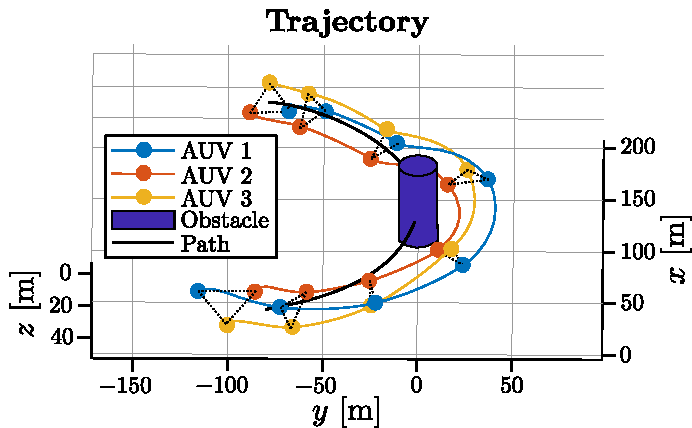
\includegraphics[width=.75\linewidth]{figures/handpos_nsb/3d_plot_alternative_view.pdf}
       \caption{The trajectory of the vehicles. The markers represent the vehicle positions every 50 seconds.}
       \label{fig:3d_plot}
   \end{subfigure}
    \begin{subfigure}[t]{.48\textwidth}
    \centering
    \def\figurewidth{.75\linewidth}
    \def\figureheight{2.5cm}
    % This file was created by matlab2tikz.
%
%The latest updates can be retrieved from
%  http://www.mathworks.com/matlabcentral/fileexchange/22022-matlab2tikz-matlab2tikz
%where you can also make suggestions and rate matlab2tikz.
%
\definecolor{mycolor1}{rgb}{0.00000,0.44700,0.74100}%
\definecolor{mycolor2}{rgb}{0.85000,0.32500,0.09800}%
\definecolor{mycolor3}{rgb}{0.92900,0.69400,0.12500}%
%
\begin{tikzpicture}

\begin{axis}[%
width=\figurewidth,
height=\figureheight,
scale only axis,
xmin=0,
xmax=350,
xlabel style={font=\color{white!15!black}},
xlabel={$t$ [s]},
ymin=-0.2,
ymax=0.25,
ylabel style={font=\color{white!15!black}, yshift=-2mm},
ylabel={Angular rate [rad/s]},
axis background/.style={fill=white},
title style={font=\bfseries, yshift=-2mm},
title={Angular velocities},
axis background/.style={fill=white},
legend style={legend cell align=left, align=left, draw=white!15!black, font=\small},
legend columns=3
]
\addplot [color=mycolor1, line width=1.0pt]
  table[]{underactuated_dynamics-1.tsv};
\addlegendentry{$p$}

\addplot [color=mycolor1, line width=1.0pt, dashed, forget plot]
  table[]{underactuated_dynamics-2.tsv};
\addplot [color=mycolor1, line width=1.0pt, dotted, forget plot]
  table[]{underactuated_dynamics-3.tsv};
\addplot [color=mycolor2, line width=1.0pt]
  table[]{underactuated_dynamics-4.tsv};
\addlegendentry{$q$}

\addplot [color=mycolor2, line width=1.0pt, dashed, forget plot]
  table[]{underactuated_dynamics-5.tsv};
\addplot [color=mycolor2, line width=1.0pt, dotted, forget plot]
  table[]{underactuated_dynamics-6.tsv};
\addplot [color=mycolor3, line width=1.0pt]
  table[]{underactuated_dynamics-7.tsv};
\addlegendentry{$r$}

\addplot [color=mycolor3, line width=1.0pt, dashed, forget plot]
  table[]{underactuated_dynamics-8.tsv};
\addplot [color=mycolor3, line width=1.0pt, dotted, forget plot]
  table[]{underactuated_dynamics-9.tsv};

\addplot[area legend, dashed, draw=black, fill=green, fill opacity=0.15, forget plot]
table[] {underactuated_dynamics-10.tsv}--cycle;
\end{axis}

\end{tikzpicture}%
    \vspace*{-1.7mm}
    \caption{The angular velocities of the vehicles. }
    \label{fig:angular_velocities}
    \end{subfigure}
    \begin{subfigure}[t]{.48\textwidth}
    \centering
    \def\figurewidth{.75\linewidth}
    \def\figureheight{2.5cm}
    % This file was created by matlab2tikz.
%
%The latest updates can be retrieved from
%  http://www.mathworks.com/matlabcentral/fileexchange/22022-matlab2tikz-matlab2tikz
%where you can also make suggestions and rate matlab2tikz.
%
\definecolor{mycolor1}{rgb}{0.00000,0.44700,0.74100}%
\definecolor{mycolor2}{rgb}{0.85000,0.32500,0.09800}%
\definecolor{mycolor3}{rgb}{0.92900,0.69400,0.12500}%
%
\begin{tikzpicture}

\begin{axis}[%
width=\figurewidth,
height=\figureheight,
scale only axis,
xmin=0,
xmax=350,
xlabel style={font=\color{white!15!black}},
xlabel={$t$ [s]},
ymin=-25,
ymax=25,
ylabel style={font=\color{white!15!black}, yshift=-2mm},
ylabel={Error [m]},
axis background/.style={fill=white},
title style={font=\bfseries, yshift=-2mm},
title={Formation keeping errors},
axis background/.style={fill=white},
legend style={legend cell align=left, align=left, draw=white!15!black,font=\scriptsize}
]
\addplot [color=mycolor1, line width=1.0pt]
table[]{formation-1.tsv};
\addlegendentry{$x$-error}

\addplot [color=mycolor1, line width=1.0pt, dashed, forget plot]
table[]{formation-2.tsv};
\addplot [color=mycolor1, line width=1.0pt, dotted, forget plot]
table[]{formation-3.tsv};
\addplot [color=mycolor2, line width=1.0pt]
table[]{formation-4.tsv};
\addlegendentry{$y$-error}

\addplot [color=mycolor2, line width=1.0pt, dashed, forget plot]
table[]{formation-5.tsv};
\addplot [color=mycolor2, line width=1.0pt, dotted, forget plot]
table[]{formation-6.tsv};
\addplot [color=mycolor3, line width=1.0pt]
table[]{formation-7.tsv};
\addlegendentry{$z$-error}

\addplot [color=mycolor3, line width=1.0pt, dashed, forget plot]
table[]{formation-8.tsv};
\addplot [color=mycolor3, line width=1.0pt, dotted, forget plot]
table[]{formation-9.tsv};

\addplot[area legend, dashed, draw=black, fill=green, fill opacity=0.15, forget plot]
table[] {formation-10.tsv}--cycle;

\addplot[area legend, dashed, draw=black, fill=white!50!red, fill opacity=0.25, forget plot]
table[] {formation-11.tsv}--cycle;
\end{axis}

\end{tikzpicture}%
    \vspace*{-1.7mm}
    \caption{The formation keeping errors. }
    \label{fig:formation_keeping_error}
    \end{subfigure}
    \begin{subfigure}[t]{.48\textwidth}
    \centering
    \def\figurewidth{.75\linewidth}
    \def\figureheight{2.5cm}
    % This file was created by matlab2tikz.
%
%The latest updates can be retrieved from
%  http://www.mathworks.com/matlabcentral/fileexchange/22022-matlab2tikz-matlab2tikz
%where you can also make suggestions and rate matlab2tikz.
%
\definecolor{mycolor1}{rgb}{0.00000,0.44700,0.74100}%
\definecolor{mycolor2}{rgb}{0.85000,0.32500,0.09800}%
%
\begin{tikzpicture}

\begin{axis}[%
width=\figurewidth,
height=\figureheight,
scale only axis,
xmin=0,
xmax=350,
xlabel style={font=\color{white!15!black}},
xlabel={$t$ [s]},
ymin=0,
ymax=25,
ylabel style={font=\color{white!15!black}, yshift=-2mm},
ylabel={Distance [m]},
axis background/.style={fill=white},
title style={font=\bfseries, yshift=-2mm},
title={Smallest distances},
legend style={at={(0.99,0.02)}, inner sep=1.5pt, anchor=south east, legend cell align=left, align=left, draw=white!15!black, legend columns=2,font=\scriptsize}
]
\addplot [color=mycolor1, line width=1.0pt]
  table[]{smallest-distances-1.tsv};
\addlegendentry{Inter-vehicle}

\addplot [color=mycolor2, line width=1.0pt]
  table[]{smallest-distances-2.tsv};
\addlegendentry{Obstacle}

\addplot [color=black, dashed, line width=1.0pt]
  table[]{smallest-distances-3.tsv};
\addlegendentry{$d_{\rm COLAV}$}


\addplot[area legend, dashed, draw=black, fill=white!50!red, fill opacity=0.25, forget plot]
table[] {smallest-distances-4.tsv}--cycle;
\end{axis}

\end{tikzpicture}%

    \vspace*{-1.8mm}
    \caption{The minimum inter-vehicle and vehicle to obstacle distance.}
    \label{fig:collision_avoidance}
    \end{subfigure}
    \begin{subfigure}[t]{.48\textwidth}
    \centering
    \def\figurewidth{.75\linewidth}
    \def\figureheight{2.5cm}
    % This file was created by matlab2tikz.
%
%The latest updates can be retrieved from
%  http://www.mathworks.com/matlabcentral/fileexchange/22022-matlab2tikz-matlab2tikz
%where you can also make suggestions and rate matlab2tikz.
%
\definecolor{mycolor1}{rgb}{0.00000,0.44700,0.74100}%
\definecolor{mycolor2}{rgb}{0.85000,0.32500,0.09800}%
\definecolor{mycolor3}{rgb}{0.92900,0.69400,0.12500}%
%
\begin{tikzpicture}

\begin{axis}[%
width=\figurewidth,
height=\figureheight,
scale only axis,
xmin=0,
xmax=350,
xlabel style={font=\color{white!15!black}},
xlabel={$t$ [s]},
ymin=-20,
ymax=20,
ylabel style={font=\color{white!15!black}, yshift=-1.5mm},
ylabel={Error [m]},
axis background/.style={fill=white},
title style={font=\bfseries, yshift=-2.75mm},
title={Path following error},
legend style={legend cell align=left, align=left, draw=white!15!black,font=\scriptsize, at={(0.99, 0.01)}, anchor=south east}
]
\addplot [color=mycolor1, line width=1.0pt]
  table[]{path-following-1.tsv};
\addlegendentry{$x$-error}

\addplot [color=mycolor2, line width=1.0pt]
  table[]{path-following-2.tsv};
\addlegendentry{$y$-error}

\addplot [color=mycolor3, line width=1.0pt]
  table[]{path-following-3.tsv};
\addlegendentry{$z$-error}


\addplot[area legend, dashed, draw=black, fill=green, fill opacity=0.15, forget plot]
table[] {path-following-4.tsv}--cycle;
\end{axis}

\end{tikzpicture}%

    \vspace*{-1.7mm}
    \caption{The barycenter path-following error.}
    \label{fig:path_following_error}
    \end{subfigure}
    \caption{Simulation results of the path-following algorithm proposed in Section~\ref{sec:case_study}. The full, dashed, and dotted lines correspond to the three different vehicles. The green and red rectangles represent when obstacle avoidance and inter-vehicle COLAV is active.}
    \label{fig:sim_results}
\end{figure}

To validate the theoretical results, we perform simulations where the proposed algorithm is applied to a fleet of three \acrfullpl{lauv} \cite{sousa_LAUV_2012}. In the simulated scenario, the barycenter should follow a spiral path while avoiding collision with a stationary cylindrical-shaped obstacle with radius $\SI{10}{\meter}$, located at $[x_o,y_o] = [100,-10]$. All position variables are here given in meters. The spiral is given by
\begin{equation}
    \mathbf{p}_p(s) = \mathbf{p}_{p,0} + \bigl[s, -40 \cos(\tfrac{\pi}{100} s), 20 \sin(\tfrac{\pi}{100} s)\bigr]\T,
\end{equation}
where \begin{equation}
    \mathbf{p}_{p,0} = \bigl[ 0, -40, 35 \bigr]\T.
\end{equation}
The barycenter relative formation is given by
\begin{equation}
    \mathbf{p}_{f,1}^f = \begin{bmatrix}0 \\ 10 \\ 5\end{bmatrix}, \quad \mathbf{p}_{f,1}^f = \begin{bmatrix}0 \\ -10 \\ 5\end{bmatrix},\quad \mathbf{p}_{f,1}^f = \begin{bmatrix}0 \\ 0 \\ -10\end{bmatrix},
\end{equation}
and we want the collision avoidance task to ensure a safe distance of $\SI{10}{\meter}$ both between vehicles in the fleet and external obstacles. Therefore, the avoidance radius of the cylinder, $\mathbf{r}_o$, is $\SI{20}{\meter}$. The vehicles are subject to an ocean current 
\begin{equation}
    \ocean = \begin{bmatrix}
        0 & 0.25 & 0.05
    \end{bmatrix}\T \,\mathrm{m/s}.
\end{equation}

The resulting trajectory of the mission is shown in \figref{fig:3d_plot}. The vehicles avoid the obstacle with a margin and return to the desired path. \figref{fig:angular_velocities} shows that the angular velocities remain bounded, in accordance with Proposition~\ref{prop:angular_velocities}. \figref{fig:formation_keeping_error} shows that the fleet converges to the desired formation while the obstacle avoidance mode is active. Except for during the inter-vehicle collision avoidance, the convergence seems linear, which can be expected because the task velocity is saturated by $v_{2,\max}$. \figref{fig:collision_avoidance} shows that the inter-vehicle \gls{colav} task activates when the distance between vehicles is below $d_{COLAV}$, and the distance does not decrease further. Because the obstacle avoidance radius $r_o$ was chosen $10 \mathrm{m}$ wider than the obstacle, the obstacle is avoided with a $10 \mathrm{m}$ margin. \figref{fig:path_following_error} shows that the path-following error initially increases as the fleet avoids the obstacle because the $x$- and $y$-components of $\mathbf{v}_{LOS,d}$ and $\dot{\mathbf{v}}_{LOS,d}$ are replaced with $\mathbf{v}_{OA,d}$ and $\dot{\mathbf{v}}_{OA,d}$ given by \eqref{eq:v_OA}, \eqref{eq:v_OA_dot}. As expected from Theorem~\ref{theorem:path_error}, the error converges to zero after the obstacle is passed when the LOS task is activated again.


\chapter{Concluding Remarks}
\label{part:conclusions}

\setlength{\epigraphwidth}{0.46\textwidth}
\epigraph{ \it
    We know everything, that is, \\
    that we know nothing.
}{
    L. Smoljak, ``Vyšetřování ztráty třídní knihy,'' 1967 (translated from Czech).
}

\chapter*{\bibname}
\printbibliography[heading=none]

\appendix
\chapter{AUV Model}
This appendix lists the equations that are too extensive to be included in the main body of the thesis.
\allowdisplaybreaks

\section{The Component Form}
\label{app:component_form}
\subsection{6\gls{dof} Model}
The functions $F_u$, $X_v$, $Y_v$, $Z_v$, $X_w$, $Y_w$, $Z_w$, $G$, $F_p$, $F_q$, and $F_r$ in \eqref{eq:background_component_form} in Section~\ref{sec:model_component} are given by
\begin{subequations}
    \begin{align}
        F_u(\cdot) &= -\frac{m_{35}q^2+m_{33}w_rq-m_{26}r^2-m_{22}v_rr+d_{11}u_r}{m_{11}}, \\
        X_v(\cdot) &= - \frac{d_{26}m_{66} - d_{66}m_{26} + u_r\left(m_{11}m_{66} - m_{26}^2\right)}{m_{22}m_{66} - m_{26}^2}, \\
        Y_v(\cdot) &= - \frac{d_{22}m_{66} - d_{62}m_{26} + u_r\left(m_{11}m_{26} - m_{22}m_{26}\right)}{m_{22}m_{66} - m_{26}^2}, \\
        Z_v(\cdot) &= \frac{p\left(m_{26}m_{35} + m_{33}m_{66}\right)}{m_{22}m_{66} - m_{26}^2}, \\
        X_w(\cdot) &= - \frac{d_{35}m_{55} - d_{55}m_{35} - u_r\left(m_{11}m_{55} - m_{36}^2\right)}{m_{33}m_{55} - m_{35}^2}, \\
        Y_w(\cdot) &= - \frac{d_{33}m_{55} - d_{53}m_{35} - u_r\left(m_{11}m_{35} - m_{33}m_{35}\right)}{m_{33}m_{55} - m_{35}^2}, \\
        Z_w(\cdot) &= - \frac{p\left(m_{26}m_{35} + m_{22}m_{55}\right)}{m_{33}m_{55} - m_{35}^2}, \\
        G(\cdot) &= -\frac{m_{35}}{m_{33}m_{55} - m_{35}^2} W z_{gb} \left[0, 1, 0\right] \left(\mat{e}_3 \times \mat{R}\T \mat{e}_3\right) \\
        F_p(\cdot) &= -\frac{d_{44}p-m_{55}qr+m_{66}qr+m_{26}qv_r+m_{35}qv_r-m_{26}rw_r}{m_{44}} \\
        &\quad + \frac{m_{35}rw_r+m_{22}v_rw_r-m_{33}v_rw_r + W z_{gb} \left[1, 0, 0\right] \left(\mat{e}_3 \times \mat{R}\T \mat{e}_3\right)}{m_{44}}, \nonumber \\
        F_q(\cdot) &= \frac{m_{33}^2u_rw_r+d_{35}m_{35}q-d_{55}m_{33}q+d_{33}m_{35}w_r-d_{53}m_{33}w_r}{m_{33}m_{55}-{m_{35}}^2} \\
        &\quad + \frac{m_{26}m_{35}pr-m_{33}m_{44}pr+m_{33}m_{66}pr-m_{11}m_{35}qu_r}{m_{33}m_{55}-{m_{35}}^2} \nonumber \\
        &\quad + \frac{m_{22}m_{35}pv_r+m_{26}m_{33}pv_r+m_{33}m_{35}qu_r}{m_{33}m_{55}-{m_{35}}^2} \nonumber \\
        &\quad + \frac{m_{11}m_{33}u_rw_r+m_{33} W z_{gb} \left[0, 1, 0\right] \left(\mat{e}_3 \times \mat{R}\T \mat{e}_3\right)}{m_{33}m_{55}-{m_{35}}^2}, \nonumber \\
        F_r(\cdot) &= -\frac{m_{22}^2u_rv_r-d_{26}m_{26}r+d_{66}m_{22}r-d_{22}m_{26}v_r}{m_{22}m_{66}-{m_{26}}^2} \\
        &\quad - \frac{d_{62}m_{22}v_r+m_{26}m_{35}pq-m_{22}m_{44}pq+m_{22}m_{55}pq}{m_{22}m_{66}-{m_{26}}^2} \nonumber \\
        &\quad - \frac{m_{22}m_{26}ru_r-m_{11}m_{26}ru_r+m_{22}m_{35}pw_r}{m_{22}m_{66}-{m_{26}}^2} \nonumber \\
        &\quad - \frac{m_{26}m_{33}pw_r-m_{11}m_{22}u_rv_r}{m_{22}m_{66}-{m_{26}}^2}. \nonumber
    \end{align}
\end{subequations}

\subsection{3\gls{dof} Model}
The functions $F_u$, $X_v$, $Y_v$, and $F_r$ in \eqref{eq:background_component_form_3DOF} are given by
\begin{subequations}
    \begin{align}
        F_u(\cdot) &= \frac{m_{23}r^2+m_{22}v_{r}r-d_{11}u_{r}}{m_{11}}, \\
        X_v(\cdot) &= \frac{(m_{23}^2 + m_{11}m_{33})u_{r}+d_{33}m_{23}-d_{23}m_{33}}{m_{22}m_{33}-m_{23}^2}, \\
        Y_v(\cdot) &= \frac{d_{22}m_{33}-d_{32}m_{23}+(m_{11}m_{23}-m_{22}m_{23})u_{r}}{m_{22}m_{33}-m_{23}^2}, \\
        F_r(\cdot) &= -\frac{m_{22}^2u_{r}v_{r}-d_{23}m_{23}r+d_{33}m_{22}r-d_{22}m_{23}v_{r}+d_{32}m_{22}v_{r}}{m_{22}m_{33}-m_{23}^2} \\
        &\quad - \frac{m_{22}m_{23}ru_{r}-m_{11}m_{23}ru_{r}-m_{11}m_{22}u_{r}v_{r}}{m_{22}m_{33}-m_{23}^2}. \nonumber
    \end{align}
\end{subequations}
\chapter{Proofs of Lemmas from Chapter \ref{chap:5dof_nsb}}

\section{Derivation of Closed-Loop Barycenter Kinematics}
\label{app:5dof_nsb_barycenter}
We begin by taking $\dot{y}_b^p$ from \eqref{eq:nsb_5dof_y_pb}.
\begin{align}
    \dot{y}_b^p &= \frac{1}{n}\sum_{i=1}^n U_i\,\cos\left(\gamma_i\right)\,\sin\left(\chi_i - \psi_p\right) - \dot{\xi}\,\iota\,x_b^p. \label{eq:nsb_5dof_y_pb_0}
\end{align}
Now, consider the term $\sin\left(\chi_i - \psi_p\right)$.
The course of the vessel is given by
\begin{align}
    \chi_i &= \psi_i + \beta_i, &
    \beta_i &= \arcsin\left(\frac{v_i}{U_i}\right).
\end{align}
After substituting and applying some trigonometric identities, we get
\begin{subequations}
    \begin{align}
        \sin\left(\chi_i - \psi_p\right) &= \sin\left(\psi_i + \beta_i - \psi_p\right) \\
        &= \cos\left(\psi_i - \psi_p\right)\,\sin\left(\beta_i\right) + \sin\left(\psi_i - \psi_p\right)\,\cos\left(\beta_i\right) \\
        &= \cos\left(\psi_i - \psi_p\right)\frac{v_i}{U_i} + \sin\left(\psi_i - \psi_p\right)\frac{\sqrt{u_i^2 + w_i^2}}{U_i}.
    \end{align}
\end{subequations}
Consequently, the term $U_i\,\cos\left(\gamma_i\right)\,\sin\left(\chi_i - \psi_p\right)$ is equivalent to
\begin{equation}
    \begin{split}
        U_i\,\cos\left(\gamma_i\right)\,\sin\left(\chi_i - \psi_p\right) = \cos\left(\gamma_i\right) \bigg(&\cos\left(\psi_i - \psi_p\right)v_i \\
        & \quad + \sin\left(\psi_i - \psi_p\right)\sqrt{u_i^2 + w_i^2}\bigg). 
    \end{split}
    \label{eq:nsb_5dof_y_pb_1}
\end{equation}

\noindent Now, consider a term $\sin\left(\psi_i + \beta_{d,i} - \psi_p\right)$.
Using a similar procedure, we get
\begin{equation}
    \sin\left(\psi_i + \beta_{d,i} - \psi_p\right) = \cos\left(\psi_i - \psi_p\right)\frac{v_i}{U_{d,i}} + \sin\left(\psi_i - \psi_p\right)\frac{\sqrt{u_{d,i}^2 + w_i^2}}{U_{d,i}}. \label{eq:nsb_5dof_y_pb_2}
\end{equation}
Combining \eqref{eq:nsb_5dof_y_pb_1} and \eqref{eq:nsb_5dof_y_pb_2}, we get
\begin{equation}
    \begin{split}
    U_i\,\cos\left(\gamma_i\right)\,\sin\left(\chi_i - \psi_p\right) &= U_{d,i}\,\cos\left(\gamma_i\right)\,\sin\left(\psi_i + \beta_{d,i} - \psi_p\right) \\
    &\, +\! \cos\left(\gamma_i\right)\sin\left(\psi_{i\!} - \psi_p\right) \! \left(\!\sqrt{u_i^2\! + \!w_i^2} -\! \sqrt{u_{d,i}^2\! + w_i^2}\right). 
    \end{split}
    \label{eq:nsb_5dof_y_pb_3}
\end{equation}
Note that the following holds for the angles
\begin{equation}
    \begin{split}
        \psi_i + \beta_{d,i} - \psi_p &= \psi_{d,i} + \tilde{\psi}_i + \beta_{d,i} - \left(\psi_{d,i} + \beta_{d,i} + \beta_{\rm LOS}\right) = \tilde{\psi}_i - \beta_{\rm LOS}, \\
        \beta_{\rm LOS} &= \scale[1]{\arctan\left(\frac{y_b^p}{\Delta\left(\mat{p}_b^p\right)}\right)}.
    \end{split}
\end{equation}
Therefore, their sine is given by
\begin{equation}
    \sin\left(\psi_i + \beta_{d,i} - \psi_p\right) = \sin\left(\tilde{\psi}_i\right)\,\scale[1]{\frac{\Delta\left(\mat{p}_b^p\right)}{\sqrt{\Delta\left(\mat{p}_b^p\right)^2 + \left(y_b^p\right)^2}}} - \cos\left(\tilde{\psi}_i\right)\scale[1]{\frac{y_b^p}{\sqrt{\Delta\left(\mat{p}_b^p\right)^2 + \left(y_b^p\right)^2}}}.
    \label{eq:nsb_5dof_sin_psi_beta}
\end{equation}
Furthermore, note that the following holds for the flight-path angle
\begin{equation}
    \gamma_i = \theta_i - \alpha_i = \tilde{\theta}_i + \theta_{d,i} - \alpha_i = \tilde{\theta}_i + \gamma_{\rm LOS} + \alpha_{d,i} - \alpha_i.
\end{equation}
Consequently, the cosine of the flight-path angle is equal to
\begin{equation}
    \begin{split}
    \cos\left(\gamma_i\right) &= \cos\left(\gamma_{\rm LOS}\right)\cos\left(\tilde{\theta}_i\right)\cos\left(\alpha_{d,i} - \alpha_i\right) \\
        &\quad - \cos\left(\gamma_{\rm LOS}\right)\sin\left(\tilde{\theta}_i\right)\sin\left(\alpha_{d,i} - \alpha_i\right) \\
        & \quad - \sin\left(\gamma_{\rm LOS}\right)\cos\left(\tilde{\theta}_i\right)\sin\left(\alpha_{d,i} - \alpha_i\right) \\
        & \quad - \sin\left(\gamma_{\rm LOS}\right)\sin\left(\tilde{\theta}_i\right)\cos\left(\alpha_{d,i} - \alpha_i\right)
    \end{split}
    \label{eq:nsb_5dof_cos_gamma_i}
\end{equation}
Using the equalities \eqref{eq:nsb_5dof_sin_psi_beta}, \eqref{eq:nsb_5dof_cos_gamma_i}, we can rewrite \eqref{eq:nsb_5dof_y_pb_3} as
\begin{equation}
    \begin{split}
        U_i\,\cos\left(\gamma_i\right)\,\sin\left(\chi_i - \psi_p\right) &= - U_{d,i}\cos\left(\gamma_{\rm LOS}\right)\scale[1]{\frac{y_b^p}{\sqrt{\Delta\left(\mat{p}_b^p\right)^2 + \left(y_b^p\right)^2}}} \\
        & \quad + G_{y,i}\left(\tilde{u}_i, \tilde{\psi}_i, \gamma_i, u_{d,i}, v_i, w_i, \mat{p}_b^p, \psi_p\right),
    \end{split}
    \label{eq:nsb_5dof_y_pb_4}
\end{equation}
where
\begin{equation}
    \begin{split}
        G_{y,i}(\cdot) &= \cos\left(\gamma_i\right)\,\sin\left(\psi_i - \psi_p\right)\left(\sqrt{u_i^2 + w_i^2} - \sqrt{u_{d,i}^2 + w_i^2}\right) \\
        &\quad - U_{d,i}\cos\left(\gamma_i\right)\,\sin\left(\tilde{\psi}_i\right)\scale[1]{\frac{\Delta\left(\mat{p}_b^p\right)}{\sqrt{\Delta\left(\mat{p}_b^p\right)^2 + \left(y_b^p\right)^2}}} \\
        &\quad + U_{d,i}\bigg[\sin\!\left(\gamma_{\rm LOS}\right)\!\left(\cos\!\left(\tilde{\theta}_i\right)\!\sin\!\left(\alpha_{d,i} - \alpha_i\right) + \sin\!\left(\tilde{\theta}_i\right)\!\cos\!\left(\alpha_{d,i} - \alpha_i\right)\right) \\
        & \qquad \qquad -\cos\left(\gamma_{\rm LOS}\right)\left(\cos\left(\tilde{\theta}_i\right)\cos\left(\alpha_{d,i} - \alpha_i\right) - 1\right)\bigg]\scale[1]{\frac{y_b^p}{\sqrt{\Delta\left(\mat{p}_b^p\right)^2 + \left(y_b^p\right)^2}}} 
    \end{split} \label{eq:nsb_5dof_G_y}
\end{equation}

\noindent Substituting \eqref{eq:nsb_5dof_y_pb_4} into \eqref{eq:nsb_5dof_y_pb_0}, we get the following
\begin{equation}
    \begin{split}
        \dot{y}_b^p &= - \frac{1}{n}\sum_{i=1}^n U_{d,i}\cos\left(\gamma_{\rm LOS}\right)\scale[1]{\frac{y_b^p}{\sqrt{\Delta\left(\mat{p}_b^p\right)^2 + \left(y_b^p\right)^2}}} - \dot{\xi}\,\iota\,x_b^p \\
        &\quad + G_y\bigg(\tilde{u}_1, \ldots, \tilde{u}_n, \tilde{\psi}_1, \ldots, \tilde{\psi}_n, \gamma_1, \ldots, \gamma_n, u_{d,1}, \ldots, u_{d,n}, \\
        & \qquad \qquad \quad v_1, \ldots, v_n, w_1, \ldots, w_n, \mat{p}_b^p, \psi_p\bigg),
    \end{split}
\end{equation}
where
\begin{equation}
    G_y(\cdot) = \frac{1}{n} \sum_{i=1}^n G_{y,i}\left(\tilde{u}_i, \tilde{\psi}_i, \gamma_i, u_{d,i}, v_i, w_i, \mat{p}_b^p, \psi_p\right).
\end{equation}

Now, we demonstrate a similar procedure for $\dot{z}_b^p$.
From \eqref{eq:nsb_5dof_y_pb}, we get
\begin{equation}
    \begin{split}
        \dot{z}_b^p &= \frac{1}{n} \sum_{i=1}^n U_i \left(-\cos\left(\theta_p\right)\sin\left(\gamma_i\right) + \cos\left(\gamma_i\right)\sin(\theta_p)\cos\left(\psi_p-\chi_i\right)\right) + \dot{\xi}\,\kappa\,x_b^p \\
        &= \frac{1}{n} \sum_{i=1}^n U_i \left(-\sin\left(\gamma_i - \theta_p\right) - \left(1 - \cos\left(\chi_i - \psi_p\right)\right)\cos\left(\gamma_i\right)\sin(\theta_p)\right) + \dot{\xi}\,\kappa\,x_b^p. 
    \end{split} \label{eq:nsb_5dof_z_pb_1}
\end{equation}
Once again, we consider the terms
\begin{equation}
    \sin\left(\gamma_i - \theta_p\right) = \sin\left(\theta_i - \alpha_i - \theta_p\right) = \sin\left(\theta_i - \theta_p\right)\frac{u_i}{U_i} - \cos\left(\theta_i - \theta_p\right)\frac{w_i}{U_i},
\end{equation}
and
\begin{equation}
    \sin\left(\theta_i - \alpha_{d,i} - \theta_p\right) = \sin\left(\theta_i - \theta_p\right)\frac{u_{d,i}}{U_{d,i}} - \cos\left(\theta_i - \theta_p\right)\frac{w_i}{U_{d,i}},
\end{equation}
which give us the following equality
\begin{equation}
    U_i\,\sin\left(\gamma_i - \theta_p\right) = U_{d,i}\,\sin\left(\theta_i - \alpha_{d,i} - \theta_p\right) + \tilde{u}_i\,\sin\left(\theta_i - \theta_p\right).
\end{equation}
Using a similar trick, we can write the sine as
\begin{equation}
    \sin\left(\theta_i - \alpha_{d,i} - \theta_p\right) = \sin\!\left(\tilde{\theta}_i\right)\!\frac{\Delta\!\left(\mat{p}_b^p\right)}{\sqrt{\Delta\!\left(\mat{p}_b^p\right)^2\! +\! \left(z_b^p\right)^2}} -\, \cos\!\left(\tilde{\theta}_i\right)\!\frac{\left(z_b^p\right)}{\sqrt{\Delta\!\left(\mat{p}_b^p\right)^2 \!+\! \left(z_b^p\right)^2}}
\end{equation}
Consequently, we can rewrite \eqref{eq:nsb_5dof_z_pb_1} as
\begin{equation}
    \begin{split}
        \dot{z}_b^p &= - \frac{1}{n} \sum_{i=1}^n U_{d,i}\frac{z_b^p}{\sqrt{\Delta\left(\mat{p}_b^p\right)^2 + \left(z_b^p\right)^2}} + \dot{\xi}\,\kappa\,x_b^p \\
        & \quad + G_z\bigg(\tilde{u}_1, \ldots, \tilde{u}_n, \tilde{\theta}_1, \ldots, \tilde{\theta}_n, \gamma_1, \ldots, \gamma_n, \chi_1, \ldots, \chi_n, \\
        & \qquad \qquad \quad u_{d,1}, \ldots, u_{d,n}, v_1, \ldots, v_n, w_1, \ldots, w_n, \mat{p}_b^p, \theta_p, \psi_p\bigg),
    \end{split}
\end{equation}
where
\begin{align}
    G_z(\cdot) &= \frac{1}{n} \sum_{i=1}^n G_{z,i}\left(\tilde{u}_i, \tilde{\theta}_i, \gamma_i, \chi_i, u_{d,i}, v_i, w_i, \mat{p}_b^p, \theta_p, \psi_p\right), \\
    \begin{split}
        G_{z,i}(\cdot) &= -U_i\left(\left(1 - \cos\left(\chi_i - \psi_p\right)\right)\cos\left(\gamma_i\right)\sin(\theta_p)\right) - \tilde{u}_i\,\sin\left(\theta_i - \theta_p\right) \\
        & \quad -\! \left(1 - \cos\!\left(\tilde{\theta}_{i\!}\right)\right)\!\frac{\left(z_b^p\right)}{\sqrt{\Delta\!\left(\mat{p}_b^p\right)^2\! +\! \left(z_b^p\right)^2}} - U_{d,i}\sin\!\left(\tilde{\theta}_i\right)\!\frac{\Delta\!\left(\mat{p}_b^p\right)}{\sqrt{\Delta\!\left(\mat{p}_b^p\right)^2\! +\! \left(z_b^p\right)^2}}.
    \end{split} \label{eq:nsb_5dof_G_z}
\end{align}

\section{Desired Pitch and Yaw Rate}
For further calculations, we need to evaluate the desired pitch ($q_{d,i}$) and yaw ($r_{d,i}$) rates of the vessels.
From \eqref{eq:nsb_5dof_theta_dot}, we get the following relation between the yaw rate and the derivative of the yaw angle
\begin{equation}
    q_{d,i} = \dot{\theta}_{d,i}.
\end{equation}
Now, we consider the desired pitch angle from \eqref{eq:nsb_5dof_theta_d}.
Since we are investigating the path following task, we substitute $\gamma_{\rm LOS}$ from \eqref{eq:nsb_5dof_v_LOS} for $\gamma_{{\rm NSB}, i}$.
Differentiating \eqref{eq:nsb_5dof_theta_d} with respect to time yields
\begin{equation}
    q_{d,i} = \dot{\theta}_p(\xi) + \frac{\Delta\left(\mat{p}_b^p\right)\,\dot{z}_b^p - z_b^p\,\dot{\Delta}\left(\mat{p}_b^p\right)}{\Delta\left(\mat{p}_b^p\right)^2 + \left(z_b^p\right)^2} + \frac{u_{d,i}\,\dot{w}}{u_{d,i}^2 + w_i^2},
\end{equation}
which can be expanded to
\begin{equation}
    \begin{split}
        q_{d,i} &= \dot{\xi}\,\kappa(\xi) + \frac{\Delta\left(\mat{p}_b^p\right)\left(\frac{1}{n} \sum\limits_{j=1}^n U_{d,j}\frac{\left(z_b^p\right)}{\sqrt{\Delta\left(\mat{p}_b^p\right)^2 + \left(z_b^p\right)^2}} + \dot{\xi}\,\kappa\,x_b^p + G_z(\cdot)\right)}{\Delta\left(\mat{p}_b^p\right)^2 + \left(z_b^p\right)^2} \\
        &\quad + \frac{z_b^p\!\left(\!-k_{\xi}\frac{\left(x_b^p\right)^2}{\sqrt{1+\left(x_b^p\right)^2}} - \frac{1}{n}\!\sum\limits_{j=1}^n \!U_{d,j}\!\left(\!\scale[1]{\frac{\cos\left(\gamma_{{\rm LOS},j}\right)^2\left(y_b^p\right)^2}{\sqrt{\Delta\left(\mat{p}_b^p\right)^2 + \left(y_b^p\right)^2}}}\! + \!\frac{\left(z_b^p\right)^2}{\sqrt{\Delta\left(\mat{p}_b^p\right)^2 + \left(z_b^p\right)^2}}\!\right)\right)}{\Delta\left(\mat{p}_b^p\right)\left(\Delta\left(\mat{p}_b^p\right)^2 + \left(z_b^p\right)^2\right)} \\
        &\quad + \frac{z_b^p\!\left(y_b^p\,G_y(\cdot) \!+\! z_b^p\,G_z(\cdot)\right)}{\Delta\!\left(\mat{p}_b^p\right)\!\left(\Delta\!\left(\mat{p}_b^p\right)^2 \!+\! \left(z_b^p\right)^2\right)} \\
        & \quad + u_{d,i}\frac{X_w\!\left(u_{d,i}+\tilde{u}_i, u_c\right)\!q + Y_w\!\left(u_{d,i}+\tilde{u}_i, u_c\right)\!\left(w_i - w_c\right)}{u_{d,i}^2 + w_i^2}.
    \end{split}
    \label{eq:nsb_5dof_q_d}
\end{equation}

From \eqref{eq:nsb_5dof_psi_dot}, we get the following relation between the yaw rate and the derivative of the yaw angle
\begin{equation}
    r_{d,i} = \dot{\psi}_{d,i}\,\cos\left(\theta_{d,i}\right).
\end{equation}
Substituting the time-derivative of \eqref{eq:nsb_5dof_psi_d}, we get
\begin{subequations}
    \begin{align}
        r_{d,i} &= \left(\dot{\psi}_p(\xi) - \frac{\Delta\!\left(\mat{p}_b^p\right)\,\dot{y}_b^p - y_b^p\,\dot{\Delta}\left(\mat{p}_b^p\right)}{\Delta\!\left(\mat{p}_b^p\right)^2 + \left(y_b^p\right)^2} - \frac{\dot{v}}{\sqrt{U_{d,i}^2 - v_i^2}}\right)\,\cos\left(\theta_{d,i}\right) \\
        \begin{split}
            &= \left[\dot{\xi}\,\iota(\xi) - \frac{\Delta\!\left(\mat{p}_b^p\right)\left(\frac{1}{n} \sum\limits_{j=1}^n U_{d,i}\frac{\cos\left(\gamma_{\rm LOS}\right)\left(y_b^p\right)}{\sqrt{\Delta\!\left(\mat{p}_b^p\right)^2 + \left(y_b^p\right)^2}} - \dot{\xi}\,\iota\,x_b^p + G_y(\cdot)\right)}{\Delta\!\left(\mat{p}_b^p\right)^2 + \left(y_b^p\right)^2} \right. \\
            &\qquad + \frac{y_b^p\!\left(\!-k_{\xi}\frac{\left(x_b^p\right)^2}{\sqrt{1+\left(x_b^p\right)^2}} - \frac{1}{n}\!\sum\limits_{j=1}^n\! U_{d,i}\!\!\left(\!\scale[1]{\frac{\cos\left(\gamma_{\rm LOS}\right)^2\left(y_b^p\right)^2}{\sqrt{\Delta\left(\mat{p}_b^p\right)^2 + \left(y_b^p\right)^2}}} +\! \frac{\left(z_b^p\right)^2}{\sqrt{\Delta\!\left(\mat{p}_b^p\right)^2\! + \left(z_b^p\right)^2}}\right)\!\right)}{\Delta\!\left(\mat{p}_b^p\right)\left(\Delta\!\left(\mat{p}_b^p\right)^2 + \left(y_b^p\right)^2\right)} \\
            &\qquad + \frac{y_b^p \left(y_b^p\,G_y(\cdot) + z_b^p\,G_z(\cdot)\right)}{\Delta\!\left(\mat{p}_b^p\right)\left(\Delta\!\left(\mat{p}_b^p\right)^2 + \left(y_b^p\right)^2\right)} \\
            &\qquad \left. -\frac{X\left(u_{d,i}+\tilde{u}_i, u_c\right)\,r + Y\left(u_{d,i}+\tilde{u}_i, u_c\right)\left(v_i - v_c\right)}{\sqrt{u_{d,i}^2 + w_i^2}} \right]\, \cos\left(\theta_{d,i}\right).
        \end{split}
    \end{align} \label{eq:nsb_5dof_r_d}
\end{subequations}

\section{Proof of Lemma \ref{lemma_1}}
\label{app:5dof_nsb_lemma_1}
In \cite{moe_LOS_2016}, it is shown that the error states \eqref{eq:nsb_5dof_u_tilde}--\eqref{eq:nsb_5dof_psi_tilde} are UGES and the ocean current estimate errors \eqref{eq:nsb_5dof_V_c_tilde}--\eqref{eq:nsb_5dof_theta_r_tilde} are bounded, which implies that \eqref{eq:nsb_5dof_u_tilde}--\eqref{eq:nsb_5dof_theta_r_tilde} are forward complete.
Therefore, we only need to prove that the underactuated sway and heave dynamics \eqref{eq:nsb_5dof_v_dot}, \eqref{eq:nsb_5dof_w_dot} and the barycenter dynamics \eqref{eq:nsb_5dof_x_pb_CL}--\eqref{eq:nsb_5dof_z_pb_CL} are forward complete.

First, let us consider the underactuated sway dynamics.
From \eqref{eq:nsb_5dof_v_dot}, we get
\begin{equation}
    \dot{v}_i = X_v\left(\tilde{u}_i + u_{d,i}, u_c\right)\,\left(\tilde{r}_i + r_{d,i}\right) + Y_v\left(\tilde{u}_i + u_{d,i}, u_c\right)\,\left(v_i - v_c\right),
\end{equation}
where $\tilde{r}_i = r_i - r_{d,i}$.
Now, let us consider a Lyapunov function candidate
\begin{equation}
    V_v(v_i) = \frac{1}{2} v_i^2. \label{eq:nsb_5dof_V_v}
\end{equation}
Its derivative along the trajectories of $v_i$ is
\begin{equation}
    \dot{V}_v(v_i) = X_v\!\left(\tilde{u}_i + u_{d,i}, u_c\right)\left(\tilde{r}_i + r_{d,i}\right)v_i + Y_v\!\left(\tilde{u}_i + u_{d,i}, u_c\right)\left(v_i - v_c\right)v_i. \label{eq:nsb_5dof_V_v_dot}
\end{equation}
From the boudedness of $\tilde{\mat{X}}_{2,i}$, $\kappa(\xi)$, $\iota(\xi)$, $u_{d,i}$, $u_c$ and $v_c$, we can conclude that there exists some scalar $\beta_{v,0} > 0$ such that
\begin{equation}
    \left\| \left[ \tilde{\mat{X}}_{2,i}\T, \kappa(\xi), \iota(\xi), u_{d,i}, u_c, v_c \right]\T \right\| \leq \beta_0.
\end{equation}
Moreover, from \eqref{eq:nsb_5dof_r_d}, we can conclude that there exist some positive functions $a_r(\beta_{v,0})$ and $b_r(\beta_{v,0})$ such that
\begin{equation}
    \abs{r_{d,i}} \leq a_r(\beta_{v,0})\,\abs{v_i} + b_r(\beta_{v,0}).
\end{equation}
Consequently, we can upper bound $\dot{V}_v(v_i)$ using the following expression
\begin{equation}
    \begin{split}
        \dot{V}_v(v_i) &\leq X_v\left(\tilde{u}_i + u_{d,i}, u_c\right)\left(\tilde{r}_i\,v_i + a_r(\cdot)v_i^2 + b_r(\cdot)v_i\right) \\
        &\quad + Y_v\left(\tilde{u}_i + u_{d,i}, u_c\right)\left(v_i^2 - v_c\,v_i\right).
    \end{split}
\end{equation}
Using Young's inequality, we get
\begin{subequations}
    \begin{align}
        \begin{split}
            \dot{V}_v(v_i) &\leq \left(X_v\left(\tilde{u}_i + u_{d,i}, u_c\right)\left(2 + a_r(\cdot)\right) + 2\,Y_v\left(\tilde{u}_i + u_{d,i}, u_c\right)\right)\,v_i^2 \\
             & \quad + X_v\left(\tilde{u}_i + u_{d,i}, u_c\right)\left(\tilde{r}_i^2 + b_r(\cdot)^2\right) + Y_v\left(\tilde{u}_i + u_{d,i}, u_c\right)\,v_c^2
        \end{split} \\
        & \leq \alpha_v\,V_v(v_i) + \beta_v.
    \end{align}
\end{subequations}
Using the comparison lemma, we get
\begin{equation}
    V_v\left(v_i(t)\right) \leq \left(V_v\left(v_i(t_0)\right) + \frac{\beta_v}{\alpha_v}\right)\,{\rm exp}\left(\alpha_v(t - t_0)\right) - \frac{\beta_v}{\alpha_v}.
\end{equation}
As $V_v(v_i)$ is defined for all $t > t_0$, it follows that $v_i$ is also defined for all $t > t_0$.
The solutions of \eqref{eq:nsb_5dof_v_dot} thus fulfill the definition of forward completeness, as defined in \cite{angeli_forward_1999}.

Now, let us consider the underactuated heave dynamics.
From \eqref{eq:nsb_5dof_w_dot}, we get
\begin{equation}
    \dot{w}_i = X_w\!\left(\tilde{u}_i + u_{d,i}, u_c\right)\left(\tilde{q}_i + q_{d,i}\right) + Y_w\!\left(\tilde{u}_i + u_{d,i}, u_c\right)\left(w_i - w_c\right) + G(\theta_i),
\end{equation}
where $\tilde{q}_i = q_i - q_{d,i}$.
Similar to the previous paragraph, we consider a Lyapunov function candidate
\begin{equation}
    V_w(w_i) = \frac{1}{2} w_i^2, \label{eq:nsb_5dof_V_w}
\end{equation}
whose derivative is
\begin{equation}
    \begin{split}
        \dot{V}_w(w_i) &= X_w\left(\tilde{u}_i + u_{d,i}, u_c\right)\,\left(\tilde{q}_i + q_{d,i}\right)\,w_i \\
        &\quad + Y_w\left(\tilde{u}_i + u_{d,i}, u_c\right)\,\left(w_i - w_c\right)\,w_i + G(\theta)\,w_i.
    \end{split}
\end{equation}
From the boudedness of $\tilde{\mat{X}}_{2,i}$, $\kappa(\xi)$, $\iota(\xi)$, $u_{d,i}$, $u_c$ and $w_c$, we can conclude that there exists some scalar $\beta_0 > 0$ such that 
\begin{equation}
    \left\| \left[ \tilde{\mat{X}}_{2,i}\T, \kappa(\xi), \iota(\xi), u_{d,i}, u_c, w_c \right]\T \right\| \leq \beta_{w,0}.
\end{equation}
Moreover, from \eqref{eq:nsb_5dof_q_d}, we can conclude that there exist some positive functions $a_q(\beta_{w,0})$ and $b_q(\beta_{w,0})$ such that
\begin{equation}
    \abs{q_{d,i}} \leq a_q(\beta_{w,0})\,\abs{w_i} + b_q(\beta_{w,0}).
\end{equation}
Consequently, we can upper bound $\dot{V}_w(w_i)$ using the following expression
\begin{equation}
    \begin{split}
        \dot{V}_w(w_i) &\leq X_w\left(\tilde{u}_i + u_{d,i}, u_c\right)\left(\tilde{q}_i\,w_i + a_q(\cdot)w_i^2 + b_q(\cdot)w_i\right) \\
        &\quad + Y_w\left(\tilde{u}_i + u_{d,i}, u_c\right)\left(w_i^2 - w_c\,w_i\right) + G(\theta_i)\,w_i.
    \end{split}
\end{equation}
Using Young's inequality, we get
\begin{equation}
    \begin{split}
        \dot{V}_w(w_i) &\leq \left(X_w\left(\tilde{u}_i + u_{d,i}, u_c\right)\left(2 + a_q(\cdot)\right) + 2\,Y_w\left(\tilde{u}_i + u_{d,i}, u_c\right) + 1\right)\,w_i^2 \\
        & \quad + X_w\left(\tilde{u}_i + u_{d,i}, u_c\right)\left(\tilde{q}_i^2 + b_q(\cdot)^2\right) + Y_w\left(\tilde{u}_i + u_{d,i}, u_c\right)\,w_c^2 + G(\theta)^2 \\
        & \leq \alpha_w\,V_w(w_i) + \beta_w.
    \end{split}
\end{equation}
Using the comparison lemma, we get
\begin{equation}
    V_w\left(w_i(t)\right) \leq \left(V_w\left(w_i(t_0)\right) + \frac{\beta_w}{\alpha_w}\right)\,{\rm exp}\left(\alpha_w(t - t_0)\right) - \frac{\beta_w}{\alpha_w}.
\end{equation}
Using the same arguments as in the previous paragraph, we conclude that the solutions of \eqref{eq:nsb_5dof_w_dot} are forward complete.

Finally, let us consider the barycenter dynamics.
We use a Lyapunov function candidate
\begin{equation}
    V_b(\mat{p}_b^p) = \frac{1}{2} \left(\left(x_b^p\right)^2 + \left(y_b^p\right)^2 + \left(z_b^p\right)^2\right),
\end{equation}
whose derivative along the solutions of \eqref{eq:nsb_5dof_x_pb_CL}--\eqref{eq:nsb_5dof_z_pb_CL} is
\begin{equation}
    \begin{split}
        \dot{V}_b\left(\mat{p}_b^p\right) &= -k_{\xi}\frac{\left(x_b^p\right)^2}{\sqrt{1 + \left(x_b^p\right)^2}} + G_y(\cdot)\,y_b^p + G_z(\cdot)\,z_b^p \\
        &\quad - \frac{1}{n}\sum_{i=1}^n U_{d,i} \left(
            \frac{\cos\left(\gamma_{\rm LOS}\right)^2\left(y_b^p\right)^2}{\sqrt{\Delta\left(\mat{p}_b^p\right)^2 + \left(y_b^p\right)^2}} +
            \frac{\left(z_b^p\right)^2}{\sqrt{\Delta\left(\mat{p}_b^p\right)^2 + \left(z_b^p\right)^2}}
        \right) \\
        &\leq G_y(\cdot)\,y_b^p + G_z(\cdot)\,z_b^p + \frac{1}{2} \left(x_b^p\right)^2.
    \end{split}
\end{equation}
Using Young's inequality, we get
\begin{equation}
    \begin{split}
        \dot{V}_b\left(\mat{p}_b^p\right) &\leq \frac{1}{2} \left(\left(x_b^p\right)^2 + \left(y_b^p\right)^2 + \left(z_b^p\right)^2\right) + \frac{1}{2}\left(G_y(\cdot)^2 + G_z(\cdot)^2\right) \\
        &\leq V_b\left(\mat{p}_b^p\right) + \frac{1}{2}\left(G_y(\cdot)^2 + G_z(\cdot)^2\right).
    \end{split}
\end{equation}
Note that from \eqref{eq:nsb_5dof_G_y} and \eqref{eq:nsb_5dof_G_z}, we can conclude that there exist some positive function $\zeta_y(U_{d,1}, \ldots, U_{d,n})$ and $\zeta_z(U_{d,1}, \ldots, U_{d,n})$ such that
\begin{align}
    \abs{G_y(\cdot)} \leq \zeta_y(\cdot) \left\| \left[\tilde{u}_1, \ldots, \tilde{u}_n, \tilde{\psi}_1, \ldots, \tilde{\psi}_n\right]\T \right\|, \\
    \abs{G_z(\cdot)} \leq \zeta_z(\cdot) \left\| \left[\tilde{u}_1, \ldots, \tilde{u}_n, \tilde{\theta}_1, \ldots, \tilde{\theta}_n\right]\T \right\|.
\end{align}
Consequently, there exists a class-$\mathcal{K}_{\infty}$ function $\zeta_p(\cdot)$ such that
\begin{equation}
    \begin{split}
        \dot{V}_p\left(\mat{p}_b^p\right) \leq V_p\left(\mat{p}_b^p\right) + \zeta_p\bigg(&v_1, \ldots, v_n, w_1, \ldots, w_n, \tilde{u}_1, \ldots, \tilde{u}_n, \\
        &\quad \tilde{\psi}_1, \ldots, \tilde{\psi}_n, \tilde{\theta}_1, \ldots, \tilde{\theta}_n\bigg).
    \end{split}
\end{equation}
Since all the arguments of $\zeta_p(\cdot)$ are forward complete, Corollary 2.11 of \cite{angeli_forward_1999} is satisfied and the barycenter dynamics is forward complete, thus concluding the proof of Lemma~\ref{lemma_1}.

\section{Proof of Lemma \ref{lemma_2}}
\label{app:5dof_nsb_lemma_2}
First, we consider the sway dynamics.
We take the Lyapunov function candidate $V_v$ from \eqref{eq:nsb_5dof_V_v} and simplify its derivative by setting $\left[\tilde{\mat{X}}_1\T, \tilde{\mat{X}}_2\T\right] = \mat{0}\T$.
\begin{equation}
    \dot{V}_v(v_i) = X_v\left(u_{d,i}, u_c\right)\,r_{d,i}\,v_i + Y_v\left(u_{d,i}, u_c\right)\,\left(v_i - v_c\right)\,v_i. \label{eq:nsb_5dof_V_v_dot_2}
\end{equation}
Next, we find an upper bound on $r_{d,i}\,v_i$.
We substitute from \eqref{eq:nsb_5dof_r_d}, set $\left[\tilde{\mat{X}}_1\T, \tilde{\mat{X}}_2\T\right] = \mat{0}\T$ and collect all terms that grow linearly with $v_i$ to obtain the following expression
\begin{align}
    \scale[0.95]{r_{d,i}\,v_i}\, &\scale[0.95]{= \!\left(\! v_i\!\left(\!1 \!+\! \frac{\Delta(\mat{p}_b^p)\,x_b^p}{\Delta(\mat{p}_b^p)^2 + \left(x_b^p\right)^2}\!\right)\! \iota(s) \frac{1}{n}\!\! \sum\limits_{j=1}^n \!U_j\Omega_x(\gamma_j, \theta_p, \chi_j, \psi_p) \!+\! \frac{Y_v(u_{d,i}, u_c)}{\sqrt{u_{d,i}^2 + w_i^2}}v_i^{2\!}\! \right)\! \cos(\theta_{d,i})} \nonumber \\
    &\quad \scale[0.95]{+ F_v(u_{d,i}, u_c, v_c, v_i, w_i, r_i, \theta_{d, i}),}
\end{align}
where
\begin{equation}
    \scale[1]{F_v(\cdot) = \frac{X_v(u_{d,i}, u_c)\,r_i - Y_v(u_{d,i}, u_c)\,v_c}{\sqrt{u_{d,i}^2 + w_i^2}} v_i \, \cos(\theta_{d,i}).}
\end{equation}
We can bound this expression as
\begin{align}
    \abs{r_{d,i}\,v_i} &\leq \frac{2}{n}\abs{v_i}\,\abs{\iota(\xi)}\sum_{j=1}^n\left(\abs{u_j} + \abs{v_j} + \abs{w_j}\right) + \abs{F_v(\cdot)} \nonumber \\
    &\leq \frac{2}{n}\abs{\iota(\xi)}\,v_i^2 + \frac{2}{n}\abs{v_i}\,\abs{\iota(\xi)}\left(\sum_{j \neq i}\bigl(\abs{u_j} + \abs{v_j} + \abs{w_j}\bigr) + \abs{u_i} + \abs{w_i}\right) \nonumber \\
    &\quad + \abs{F_v(u_{d,i}, u_c, v_c, v_i, w_i, r_i, \theta_{d, i})},
\end{align}
which we can substitute to \eqref{eq:nsb_5dof_V_v_dot_2} to obtain
\begin{equation}
    \begin{split}
        \dot{V}_v(v_i) &\leq \left(X_v\left(u_{d,i}, u_c\right)\frac{2}{n}\abs{\iota(\xi)} + Y_v\left(u_{d,i}, u_c\right)\right)v_i^2 \\
        &\quad + \left(\frac{2}{n}\abs{v_i}\,\abs{\iota(\xi)}\sum_{j \neq i}\bigl(\abs{u_j} + \abs{v_j} + \abs{w_j}\bigr) + \abs{u_i} + \abs{w_i}\right) \\
        & \quad + \left(\abs{F_v(\cdot)} - Y_v\left(u_{d,i}, u_c\right)\abs{v_c}\right) \abs{v_i}.
    \end{split}
\end{equation}
For a sufficiently large $v_i$, the quadratic term will dominate the linear term.
Therefore, we can conclude that $v_i$ is bounded if 
\begin{equation}
    X_v\left(u_{d,i}, u_c\right)\frac{2}{n}\abs{\iota(\xi)} + Y_v\left(u_{d,i}, u_c\right) < 0.
\end{equation}
Since $Y_v$ is assumed to be always negative, the inequality is satisfied if
\begin{equation}
    \abs{\iota(\xi)} < \frac{n}{2}\abs{\frac{Y_v\left(u_{d,i}, u_c\right)}{X_v\left(u_{d,i}, u_c\right)}}.
\end{equation}

Now, we perform a similar procedure for the heave dynamics.
We take the Lyapunov function candidate $V_w$ from \eqref{eq:nsb_5dof_V_w} and simplify its derivative by setting $\left[\tilde{\mat{X}}_1\T, \tilde{\mat{X}}_2\T\right] = \mat{0}\T$.
\begin{equation}
    \dot{V}_w(w_i) = X_w\left(u_{d,i}, u_c\right)\,q_{d,i}\,w_i + Y_w\left(u_{d,i}, u_c\right)\,\left(w_i - w_c\right)\,w_i + G(\theta_i)\,w_i. \label{eq:nsb_5dof_V_w_dot}
\end{equation}
Next, we find an upper bound on $q_{d,i}\,w_i$.
We substitute from \eqref{eq:nsb_5dof_q_d}, set $\left[\tilde{\mat{X}}_1\T, \tilde{\mat{X}}_2\T\right] = \mat{0}\T$ and collect all terms that grow linearly with $w_i$ to obtain the following expression
\begin{align}
    \scale[1]{q_{d,i}\,w_i}\, &\scale[1]{= w_i\left(1 + \frac{\Delta(\mat{p}_b^p)\,x_b^p}{\Delta(\mat{p}_b^p)^2 + \left(x_b^p\right)^2}\right) \kappa(\xi) \frac{1}{n} \sum\limits_{j=1}^n U_j\,\Omega_x(\gamma_j, \theta_p, \chi_j, \psi_p)} \\
    & \quad \scale[1]{+ u_{d,i}\frac{Y_w(u_{d,i}, u_c)}{u_{d,i}^2 + w_i^2}w_i^2 + F_w(u_{d,i}, u_c, w_c, w_i, q_i),}
\end{align}
where
\begin{equation}
    \scale[1]{F_w(\cdot) =  u_{d,i}\frac{X_w(u_{d,i}, u_c)\,r_i - Y_w(u_{d,i}, u_c)\,w_c}{\sqrt{u_{d,i}^2 + w_i^2}} w_i.}
\end{equation}
We can bound this expression as
\begin{equation}
    \begin{split}
        \abs{q_{d,i}\,w_i} &\leq \frac{2}{n}\abs{\kappa(\xi)}\,w_i^2 + \frac{2}{n}\abs{w_i}\,\abs{\kappa(\xi)}\left(\sum_{j \neq i}\bigl(\abs{u_j} + \abs{v_j} + \abs{w_j}\bigr) + \abs{u_i} + \abs{v_i}\right) \\
        &\quad + \abs{F_w(u_{d,i}, u_c, w_c, w_i, q_i)},
    \end{split}
\end{equation}
which we can substitute to \eqref{eq:nsb_5dof_V_w_dot} to obtain
\begin{equation}
    \begin{split}
        \dot{V}_w(w_i) &\leq \left(X_w\left(u_{d,i}, u_c\right)\frac{2}{n}\abs{\kappa(\xi)} + Y_w\left(u_{d,i}, u_c\right)\right)w_i^2 \\
        & \quad + \left(\frac{2}{n}\abs{w_i}\,\abs{\kappa(\xi)}\sum_{j \neq i}\bigl(\abs{u_j} + \abs{v_j} + \abs{w_j}\bigr) + \abs{u_i} + \abs{w_i}\right) \\
        & \quad + \left(\abs{F(\cdot)} - Y_w\left(u_{d,i}, u_c\right)\abs{v_c} + \abs{G(\theta_i)}\right) \abs{w_i} + G(\theta_i)\,w_i.
    \end{split}
\end{equation}
For a sufficiently large $w_i$, the quadratic term will dominate the linear term.
Therefore, we can conclude that $w_i$ is bounded if 
\begin{equation}
    X_w\left(u_{d,i}, u_c\right)\frac{2}{n}\abs{\kappa(\xi)} + Y_w\left(u_{d,i}, u_c\right) < 0.
\end{equation}
Since $Y_w$ is assumed to be always negative, the inequality is satisfied if
\begin{equation}
    \abs{\kappa(\xi)} < \frac{n}{2}\abs{\frac{Y_w\left(u_{d,i}, u_c\right)}{X_w\left(u_{d,i}, u_c\right)}},
\end{equation}
which concludes the proof of Lemma \ref{lemma_2}.

\section{Proof of Lemma \ref{lemma_3}}
\label{app:5dof_nsb_lemma_3}
First, we consider the sway dynamics.
We take the Lyapunov function candidate $V_v$ from \eqref{eq:nsb_5dof_V_v} and simplify its derivative by setting $\tilde{\mat{X}}_2 = \mat{0}$.
\begin{equation}
    \dot{V}_v(v_i) = X_v\left(u_{d,i}, u_c\right)\,r_{d,i}\,v_i + Y_v\left(u_{d,i}, u_c\right)\,\left(v_i - v_c\right)\,v_i. \label{eq:nsb_5dof_V_v_dot_3}
\end{equation}
Next, we find an upper bound on $r_{d,i}\,v_i$.
We substitute from \eqref{eq:nsb_5dof_r_d}, set $\tilde{\mat{X}}_2 = \mat{0}$ and collect all terms that grow linearly with $v_i$ to obtain the following expression
\begin{equation}
    \begin{split}
        {r_{d,i}\,v_i} &= \scale[1]{\left( v_i\left(1 + \frac{\Delta(\mat{p}_b^p)\,x_b^p}{\Delta(\mat{p}_b^p)^2 + \left(x_b^p\right)^2}\right) \iota(\xi) \frac{1}{n} \sum\limits_{j=1}^n U_j\,\Omega_x(\gamma_j, \theta_p, \chi_j, \psi_p) \right.} \\
        &\qquad \scale[1]{
        - \frac{y_b^p\,v_i\,\sum\limits_{j=1}^n\left(\frac{\cos\left(\gamma_{\rm LOS}\right)y_b^p}{\sqrt{\Delta\left(\mat{p}_b^p\right)^2 + \left(y_b^p\right)^2}} + \frac{z_b^p}{\sqrt{\Delta\left(\mat{p}_b^p\right)^2 + \left(z_b^p\right)^2}}\right)}{n\,\Delta(\mat{p}_b^p)\left(\Delta(\mat{p}_b^p)^2 + \left(y_b^p\right)^2\right)} } \\
        &\qquad \left. + \frac{v_i\,\Delta(\mat{p}_b^p)\sum\limits_{j=1}^n\frac{\cos\left(\gamma_{\rm LOS}\right)y_b^p}{\sqrt{\Delta\left(\mat{p}_b^p\right)^2 + \left(y_b^p\right)^2}}}{n\,\left(\Delta(\mat{p}_b^p)^2 + (y_b^p)^2\right)} + \frac{Y_v(u_{d,i}, u_c)}{\sqrt{u_{d,i}^2 + w_i^2}}v_i^2 \right) \cos(\theta_{d,i}) \\
        &\quad + H_v(u_{d,i}, \theta_{d,i}, u_c, v_c, v_i, w_i, r_i, \mat{p}_b^p, \xi),
    \end{split}
\end{equation}
\begin{equation}
    \begin{split}
        H_v(\cdot) & = \left(\left(1 + \frac{\Delta(\mat{p}_b^p)\,x_b^p}{\Delta(\mat{p}_b^p)^2 + \left(x_b^p\right)^2}\right)k_{\xi}\,\iota(\xi)\frac{x_b^p}{\sqrt{1+\left(x_b^p\right)^2}} \right. \\
        &\qquad + \frac{X_v(u_{d,i}, u_c)\,r_i - Y_v(u_{d,i}, u_c)\,v_c}{\sqrt{u_{d,i}^2 + w_i^2}}  \\
        &\qquad \left. - \frac{y_b^p\,k_{\xi}\,x_b^p}{\sqrt{1+\left(x_b^p\right)^2}\Delta(\mat{p}_b^p)\left(\Delta(\mat{p}_b^p)^2 + \left(y_b^p\right)^2\right)}  \right) v_i \, \cos(\theta_{d,i}).
    \end{split}
\end{equation}
We can bound this expression as
\begin{equation}
    \begin{split}
        \abs{r_{d,i}\,v_i} &\leq \left(\frac{2}{n}\abs{\iota(\xi)} + \frac{3}{n\,\Delta(\mat{p}_b^p)}\right)\abs{v_i}\,\sum_{j=1}^n\left(\abs{u_j} + \abs{v_j} + \abs{w_j}\right) + \abs{H_v(\cdot)} \\
        &\leq \left(\frac{2}{n}\abs{\iota(\xi)} + \frac{3}{n\,\Delta(\mat{p}_b^p)}\right)\,v_i^2 + \abs{H_v(\cdot)} \\
        &\quad + \left(\frac{2}{n}\abs{\iota(\xi)} + \frac{3}{n\,\Delta(\mat{p}_b^p)}\right)\left(\sum_{j \neq i}\bigl(\abs{u_j} + \abs{v_j} + \abs{w_j}\bigr) + \abs{u_i} + \abs{w_i}\right),
    \end{split}
\end{equation}
which we can substitute to \eqref{eq:nsb_5dof_V_v_dot_3} to obtain
\begin{equation}
    \begin{split}
        \dot{V}_v(v_i) &\leq \left(X_v\left(u_{d,i}, u_c\right)\left(\frac{2}{n}\abs{\iota(\xi)} + \frac{3}{n\,\Delta(\mat{p}_b^p)}\right) + Y_v\left(u_{d,i}, u_c\right)\right)v_i^2 \\
        & \quad + \left(\frac{2}{n}\abs{\iota(\xi)} + \frac{3}{n\,\Delta(\mat{p}_b^p)}\right)\left(\sum_{j \neq i}\bigl(\abs{u_j} + \abs{v_j} + \abs{w_j}\bigr) + \abs{u_i} + \abs{w_i}\right) \\
        & \quad + \left(\abs{H_v(\cdot)} - Y_v\left(u_{d,i}, u_c\right)\abs{v_c}\right) \abs{v_i}.
    \end{split}
\end{equation}
For a sufficiently large $v_i$, the quadratic term will dominate the linear term.
Therefore, we can conclude that $v_i$ is bounded if 
\begin{equation}
    X_v\left(u_{d,i}, u_c\right)\left(\frac{2}{n}\abs{\iota(\xi)} + \frac{3}{n\,\Delta(\mat{p}_b^p)}\right) + Y_v\left(u_{d,i}, u_c\right) < 0.
\end{equation}
From the definition of the lookahead distance \eqref{eq:nsb_5dof_delta}, this condition is satisfied if
\begin{equation}
    \Delta_0 > \frac{3}{n\abs{\frac{Y_v\left(u_{d,i}, u_c\right)}{X_v\left(u_{d,i}, u_c\right)}} - 2\abs{\iota(\xi)}}.
\end{equation}

Now, we perform a similar procedure for the heave dynamics.
We take the Lyapunov function candidate $V_w$ from \eqref{eq:nsb_5dof_V_w} and simplify its derivative by setting $\tilde{\mat{X}}_2 = \mat{0}$.
\begin{equation}
    \dot{V}_w(w_i) = X_w\left(u_{d,i}, u_c\right)\,q_{d,i}\,w_i + Y_w\left(u_{d,i}, u_c\right)\,\left(w_i - w_c\right)\,w_i + G(\theta_i)\,w_i. \label{eq:nsb_5dof_V_w_dot_2}
\end{equation}
Next, we find an upper bound on $q_{d,i}\,w_i$.
We substitute from \eqref{eq:nsb_5dof_q_d}, set $\tilde{\mat{X}}_2 = \mat{0}$ and collect all terms that grow linearly with $w_i$ to obtain the following expression
\begin{equation}
    \begin{split}
        {q_{d,i}\,w_i} &= \scale[1]{ w_i\left(1 + \frac{\Delta(\mat{p}_b^p)\,x_b^p}{\Delta(\mat{p}_b^p)^2 + \left(x_b^p\right)^2}\right) \kappa(\xi) \frac{1}{n} \sum_{j=1}^n U_j\,\Omega_x(\gamma_j, \theta_p, \chi_j, \psi_p)} \\
        &\quad \scale[1]{- \frac{z_b^p\,w_i\,\sum_{j=1}^n\left(\frac{\cos\left(\gamma_{\rm LOS}\right)y_b^p}{\sqrt{\Delta\left(\mat{p}_b^p\right)^2 + \left(y_b^p\right)^2}} + \frac{z_b^p}{\sqrt{\Delta\left(\mat{p}_b^p\right)^2 + \left(z_b^p\right)^2}}\right)}{n\,\Delta(\mat{p}_b^p)\left(\Delta(\mat{p}_b^p)^2 + \left(z_b^p\right)^2\right)} } \\
        &\quad  + \frac{w_i\,\Delta(\mat{p}_b^p)\sum_{j=1}^n\frac{z_b^p}{\sqrt{\Delta\left(\mat{p}_b^p\right)^2 + \left(z_b^p\right)^2}}}{n\,\left(\Delta(\mat{p}_b^p)^2 + (z_b^p)^2\right)} + u_{d,i}\frac{Y_w(u_{d,i}, u_c)}{{u_{d,i}^2 + w_i^2}}w_i^2 \\
        &\quad + H_w(u_{d,i}, u_c, v_c, w_i, v_i, q_i, \mat{p}_b^p, \xi),
    \end{split}
\end{equation}
where
\begin{equation}
    \begin{split}
        H_w(\cdot) & = \left(\left(1 + \frac{\Delta(\mat{p}_b^p)\,x_b^p}{\Delta(\mat{p}_b^p)^2 + \left(x_b^p\right)^2}\right)k_{\xi}\,\kappa(\xi)\frac{x_b^p}{\sqrt{1+\left(x_b^p\right)^2}} \right. \\
        & \qquad - \frac{y_b^p\,k_{\xi}\,x_b^p}{\sqrt{1+\left(x_b^p\right)^2}\Delta(\mat{p}_b^p)\left(\Delta(\mat{p}_b^p)^2 + \left(y_b^p\right)^2\right)} \\
        &\qquad \left. + u_{d,i}\frac{X_w(u_{d,i}, u_c)\,r_i - Y_w(u_{d,i}, u_c)\,v_c}{{u_{d,i}^2 + w_i^2}} \right) w_i.
    \end{split}
\end{equation}
We can bound this expression as
\begin{equation}
    \begin{split}
        \abs{q_{d,i}\,w_i} &\leq \left(\frac{2}{n}\abs{\kappa(\xi)} + \frac{3}{n\,\Delta(\mat{p}_b^p)}\right)\abs{w_i}\,\sum_{j=1}^n\left(\abs{u_j} + \abs{v_j} + \abs{w_j}\right) + \abs{H_w(\cdot)} \\
        &\leq \left(\frac{2}{n}\abs{\kappa(\xi)} + \frac{3}{n\,\Delta(\mat{p}_b^p)}\right)\,w_i^2 + \abs{H_w(\cdot)} \\
        &\quad + \left(\frac{2}{n}\abs{\kappa(\xi)} + \frac{3}{n\,\Delta(\mat{p}_b^p)}\right)\left(\sum_{j \neq i}\bigl(\abs{u_j} + \abs{v_j} + \abs{w_j}\bigr) + \abs{u_i} + \abs{w_i}\right),
    \end{split}
\end{equation}
which we can substitute to \eqref{eq:nsb_5dof_V_w_dot_2} to obtain
\begin{equation}
    \begin{split}
        \dot{V}_w(w_i) &\leq \left(X_w\left(u_{d,i}, u_c\right)\left(\frac{2}{n}\abs{\kappa(\xi)} + \frac{3}{n\,\Delta(\mat{p}_b^p)}\right) + Y_w\left(u_{d,i}, u_c\right)\right)w_i^2 \\
        & \quad + \left(\frac{2}{n}\abs{\kappa(\xi)} + \frac{3}{n\,\Delta(\mat{p}_b^p)}\right)\left(\sum_{j \neq i}\bigl(\abs{u_j} + \abs{v_j} + \abs{w_j}\bigr) + \abs{u_i} + \abs{w_i}\right) \\
        & \quad + \left(\abs{H_w(\cdot)} - Y_w\left(u_{d,i}, u_c\right)\abs{v_c}\right) \abs{w_i}.
    \end{split}
\end{equation}
For a sufficiently large $w_i$, the quadratic term will dominate the linear term.
Therefore, we can conclude that $w_i$ is bounded if 
\begin{equation}
    X_w\left(u_{d,i}, u_c\right)\left(\frac{2}{n}\abs{\kappa(\xi)} + \frac{3}{n\,\Delta(\mat{p}_b^p)}\right) + Y_w\left(u_{d,i}, u_c\right) < 0.
\end{equation}
From the definition of the lookahead distance \eqref{eq:nsb_5dof_delta}, this condition is satisfied if
\begin{equation}
    \Delta_0 > \frac{3}{n\abs{\frac{Y_w\left(u_{d,i}, u_c\right)}{X_w\left(u_{d,i}, u_c\right)}} - 2\abs{\kappa(\xi)}}.
\end{equation}

\chapter{Derivations from Chapter~\ref{chap:NSB_R}}
\label{app:NSB_R}

%\section{Bounds on $\bs{\omega}_{\bs{\upsilon}_{{\rm NSB}, i}}$}
\section{Bounds on the NSB Velocity}
\label{app:v_NSB}
Recall the definition of $\bs{\omega}_{\bs{\upsilon}_{{\rm NSB},i}}$ in \eqref{eq:NSB_R_omega_v}.
Note that by definition, a normalized vector is always orthogonal to its derivative.
Therefore, the following equality holds:
\begin{equation}
    \norm{\bs{\omega}_{\bs{\upsilon}_{{\rm NSB}, i}}} = \norm{\overline{\bs{\upsilon}}_{{\rm NSB}, i}}\norm{\dot{\overline{\bs{\upsilon}}}_{{\rm NSB}, i}}
    = \norm{\dot{\overline{\bs{\upsilon}}}_{{\rm NSB}, i}}.
\end{equation}
Therefore, instead of the pseudo-angular velocity, it is possible to investigate the derivative of the normalized NSB velocity.
Note that according to the assumptions in Theorem~\ref{thm1}, the analysis should be performed on the manifold $\left[\tilde{\bs{\sigma}}\T, \tilde{\mat{X}}\T\right] = \mat{0}\T$.
Substituting $\tilde{\bs{\sigma}} = \mat{0}$ to \eqref{eq:NSB_R_v_NSB_i} yields
\begin{equation}
    \begin{split}
        \bs{\upsilon}_{{\rm NSB}, i} &= \bs{\upsilon}_{\rm LOS} + \dot{\mat{R}}_p(\xi)\mat{p}_{f,i}^f \\
        &= U_{\rm LOS}\mat{R}_p(\xi) \left(\mat{e}_1 + \norm{\partial \mat{p}_p(\xi) / \partial \xi}^{-1}\bs{\omega}_p(\xi) \times \mat{p}_{f,i}^f\right).
    \end{split}
    \label{eq:NSB_R_v_NSB_i_nominal}
\end{equation}
For brevity, let us define
\begin{align}
    \bs{\kappa} &= \norm{\partial \mat{p}_p(\xi) / \partial \xi}^{-1}\bs{\omega}_p(\xi), &
    \mat{e}_p &= \mat{e}_1 + \bs{\kappa} \times \mat{p}_{f,i}^f
\end{align}
The normalized NSB velocity is then given by
\begin{equation}
    \overline{\bs{\upsilon}}_{{\rm NSB}, i} = \frac{\mat{R}_p(\xi) \mat{e}_p}{\norm{\mat{e}_p}}.
    \label{eq:NSB_R_v_NSB_i_normalized}
\end{equation}
Differentiating \eqref{eq:NSB_R_v_NSB_i_normalized} with respect to time yields
\begin{equation}
    \dot{\overline{\bs{\upsilon}}}_{{\rm NSB}, i} = 
    \frac{U_{\rm LOS}\mat{R}_p\left(\bs{\kappa}\times\mat{e}_p + \bs{\iota}\times\mat{p}_{f,i}^f\right)}{\norm{\mat{e}_p}}
    - \frac{U_{\rm LOS}\mat{R}_p\mat{e}_p\left(\mat{e}_p\T\left(\bs{\iota}\times\mat{p}_{f,i}^f\right)\right)}{\norm{\mat{e}_p}^2},
    \label{eq:NSB_R_v_NSB_i_dot}
\end{equation}
where $\bs{\iota} = \partial \bs{\kappa} / \partial \xi$. From \eqref{eq:NSB_R_v_NSB_i_dot}, it follows that
\begin{equation}
    \norm{\dot{\overline{\bs{\upsilon}}}_{{\rm NSB}, i}} \leq
    U_{\rm LOS} \left(\norm{\bs{\kappa}} + \frac{\norm{\bs{\iota}\times\mat{p}_{f,i}^f}\left(1 + \norm{\mat{e}_p}\right)}{\norm{\mat{e}_p}}\right).
    \label{eq:NSB_R_v_NSB_i_dot_bound1}
\end{equation}
If we assume that the second and third partial derivatives of $\mat{p}_p$ with respect to the path parameter are bounded, then $\bs{\iota}$ is bounded as well.
Let us define
\begin{equation}
    c_{\rm NSB} = \max_{i, \xi} \left(\norm{\bs{\kappa}} + \frac{\norm{\bs{\iota}\times\mat{p}_{f,i}^f}\left(1 + \norm{\mat{e}_p}\right)}{\norm{\mat{e}_p}}\right).
    \label{eq:NSB_R_c_NSB}
\end{equation}
Substituting \eqref{eq:NSB_R_U_LOS} and \eqref{eq:NSB_R_c_NSB} into \eqref{eq:NSB_R_v_NSB_i_dot_bound1} gives us the following upper bound
\begin{equation}
    \norm{\dot{\overline{\bs{\upsilon}}}_{{\rm NSB}, i}} \leq 
    \frac{\upsilon_{2, \max} + \sqrt{\sum_{i=1}^n \left(v_i^2 + w_i^2\right) + u_{\min}^2}}{1 - k_{\rm NSB}}\,c_{\rm NSB}.
    \label{eq:NSB_R_v_NSB_i_dot_bound2}
\end{equation}
Note that for any two positive numbers $a$ and $b$, the following inequality holds: $\sqrt{a + b} \leq \sqrt{a} + \sqrt{b}$.
Therefore, we can further upper-bound \eqref{eq:NSB_R_v_NSB_i_dot_bound2} with
\begin{equation}
    \norm{\dot{\overline{\bs{\upsilon}}}_{{\rm NSB}, i}} \leq 
    \underbrace{\frac{c_{\rm NSB}}{1 - k_{\rm NSB}}}_{a_{\rm NSB}}\norm{\mat{v}_u} +
    \underbrace{\frac{\upsilon_{2, \max} + u_{\min}}{1 - k_{\rm NSB}}\,c_{\rm NSB}}_{b_{\rm NSB}}.
\end{equation}
We have thus shown that there exist positive constants $a_{\rm NSB}$ and $b_{\rm NSB}$ that satisfy \eqref{eq:NSB_R_omega_NSB_bound}.

%\section{Bounds on $\bs{\omega}_{\mat{v}_i}$}
\section{Bounds on the Linear Velocity}
\label{app:omega_v}
Note that by the assumptions of Theorem~\ref{thm1}, the surge velocity of the vehicle satisfies $u_i = u_{d, i}$, and the linear velocity vector $\mat{v}_i$ thus  satisfies
\begin{align}
    \mat{v}_i &= \inlinevector{u_{d,i}, v_i, w_i} = \inlinevector{\sqrt{\norm{\bs{\upsilon}_{{\rm NSB}, i}}^2 - v_i^2 - w_i^2}, v_i, w_i}, &
    \norm{\mat{v}_i} &= \norm{\bs{\upsilon}_{{\rm NSB}, i}}.
    \label{eq:NSB_R_v_i_nominal}
\end{align}
The time-derivative of a normalized vector is given by
\begin{equation}
    \dot{\overline{\mat{v}}}_i = \frac{\dot{\mat{v}}_i}{\norm{\mat{v}_i}} - \frac{\mat{v}_i\,\,\frac{\rm d}{{\rm d}t}\!\norm{\mat{v}_i}}{\norm{\mat{v}_i}^2},
\end{equation}
and the pseudo-angular velocity is thus given by
\begin{equation}
    \bs{\omega}_{\mat{v}_i} = \overline{\mat{v}}_i \times \dot{\overline{\mat{v}}}_i
    = \frac{\mat{v}_i}{\norm{\mat{v}_i}} \times 
        \left(\frac{\dot{\mat{v}}_i}{\norm{\mat{v}_i}} - \frac{\mat{v}_i\,\,\frac{\rm d}{{\rm d}t}\!\norm{\mat{v}_i}}{\norm{\mat{v}_i}^2}\right)
    = \frac{\mat{v}_i \times \dot{\mat{v}}_i}{\norm{\mat{v}_i}^2}.
    \label{eq:NSB_R_omega_v_a1}
\end{equation}
Now, let us focus on $\dot{\mat{v}}_i$.
Differentiating \eqref{eq:NSB_R_v_i_nominal} with respect to time yields
\begin{equation}
    \dot{\mat{v}}_i = \begin{bmatrix}
        \frac{\bs{\upsilon}_{{\rm NSB}, i}\T\dot{\bs{\upsilon}}_{{\rm NSB}, i} - v_i\dot{v}_i - w_i\dot{w}_i}{u_i} \\
        \dot{v}_i \\
        \dot{w}_i
    \end{bmatrix}.
    \label{eq:NSB_R_v_i_dot}
\end{equation}
From \eqref{eq:NSB_R_underactuated_dynamics}, the underactuated dynamics are given by
\begin{subequations}
    \begin{align}
        \dot{v}_i &= \left(X_{v0} + X_{v1}(u_i-u_c)\right)r_i + \left(Y_{v0} + Y_{v1}(u_i-u_c)\right)(v_i-v_c) \nonumber \\
        &\quad + \left(Z_{v0} + Z_{v1}p_i\right)(w_i-w_c) + w_cp_i - u_cr_i, \\
        \dot{w}_i &= \left(X_{w0} + X_{w1}(u_i-u_c)\right)q_i + \left(Y_{w0} + Y_{w1}(u_i-u_c)\right)(w_i-w_c) \nonumber \\
        &\quad + \left(Z_{w0} + Z_{w1}p_i\right)(v_i-v_c) + u_cq_i - v_cp_i,
    \end{align}
    \label{eq:NSB_R_underactuated_dynamics_expanded}
\end{subequations}
where
\begin{subequations}
    \begin{align}
        X_v(u_r) &= X_{v0} + X_{v1}u_r, &
        X_w(u_r) &= X_{w0} + X_{w1}u_r, \\
        Y_v(u_r) &= Y_{v0} + Y_{v1}u_r, &
        Y_w(u_r) &= Y_{w0} + Y_{w1}u_r, \\
        Z_v(p) &= Z_{v0} + Z_{v1}p, &
        Z_w(p) &= Z_{w0} + Z_{w1}p.
    \end{align}
\end{subequations}
Substituting \eqref{eq:NSB_R_underactuated_dynamics_expanded} into \eqref{eq:NSB_R_v_i_dot} yields
\begin{equation}
    \dot{\mat{v}}_i = \mat{A}_{\bs{\omega}_i} \bs{\omega}_i + \widehat{\bs{\omega}}_{0, i},
    \label{eq:NSB_R_v_i_dot_matrix_form}
\end{equation}
where
\begin{equation}
    \begin{split}
        \mat{A}_{\bs{\omega}_i\!}\! &=\!\!
        \begin{bmatrix}
            \frac{w_{i}\,\left(v_{c}-Z_{w1}\,v_{r}\right)-v_{i}\,\left(w_{c}+Z_{v1}\,w_{r}\right)}{u_{i}} & 
            \!-\frac{w_{i}\,\left(X_{w0}+X_{w1}\,u_{r}+u_{c}\right)}{u_{i}}\! & 
            \frac{v_{i}\,\left(u_{c}-X_{v0}-X_{v1}\,u_{r}\right)}{u_{i}} \\ 
            w_{c}+Z_{v1}\,w_{r} & 0 & X_{v0\!}+\!X_{v1\!}\,u_{r\!}-u_{c} \\ 
            -v_{c}-Z_{w1}\,v_{r} & \!X_{w0\!}+\!X_{w1\!}\,u_{r\!}+u_{c\!} & 0
        \end{bmatrix} \\
        \widehat{\bs{\omega}}_{0, i}\! &=\!\!
        \begin{bmatrix}
            \frac{\bs{\upsilon}_{{\rm NSB}, i}\T\dot{\bs{\upsilon}}_{{\rm NSB}, i} 
            - v_i\left(\left(Y_{v0} + Y_{v1}u_r\right)v_r + Z_{v0}w_r\right)
            - w_i\left(\left(Y_{w0} + Y_{w1}u_r\right)w_r + Z_{w0}v_r\right)}{u_i} \\
            \left(Y_{v0} + Y_{v1}u_r\right)v_r + Z_{v0}w_r \\
            \left(Y_{w0} + Y_{w1}u_r\right)w_r + Z_{w0}v_r
    \end{bmatrix}.
    \end{split}
\end{equation}
Substituting \eqref{eq:NSB_R_v_i_dot_matrix_form} into \eqref{eq:NSB_R_omega_v_a1} yields
\begin{equation}
    \bs{\omega}_{\mat{v}_i} = \frac{\mat{v}_i \times \left(\widehat{\mat{A}}_{\bs{\omega}_i}\bs{\omega}_i + \widehat{\bs{\omega}}_{0, i}\right)}{\norm{\mat{v}_i}^2}
    = \underbrace{\frac{\mat{S}\left(\mat{v}_i\right)\widehat{\mat{A}}_{\bs{\omega}_i}}{\norm{\mat{v}_i}^2}}_{\mat{A}_{\bs{\omega}_i}}\bs{\omega}_i
     + \underbrace{\frac{\mat{v}_i \times \widehat{\bs{\omega}}_{0, i}}{\norm{\mat{v}_i}^2}}_{\bs{\omega}_{0, i}}.
     \label{eq:NSB_R_omega_v_affine}
\end{equation}
We have thus shown that $\bs{\omega}_{\mat{v}_i}$ is affine in $\bs{\omega}_i$.

Now we investigate the determinant of $(\mat{I} + \mat{A}_{\bs{\omega}_i})$.
From the definition of $\mat{A}_{\bs{\omega}_i}$ in \eqref{eq:NSB_R_omega_v_affine}, we get the following expression
\begin{align}
    \det\left(\mat{I} + \mat{A}_{\bs{\omega}_i}\right) = \bigg( &
    u_i\left(u_i^2 + v_i^2 + w_i^2\right) - u_c\left(u_i^2 + v_i^2 + w_i^2\right) \nonumber \\
    & - \left(u_cu_i + v_cv_i + w_cw_i\right)\left(u_i - u_c\right) + X_{v0}\left(u_i^2 + v_i^2\right) \nonumber \\
    & - X_{w0}\left(u_i^2 + w_i^2\right) + \left(X_{v1} - X_{w1}\right)u_i\left(u_i - u_c\right)^2 \nonumber \\
    & + \left(X_{v1} + Z_{w1}\right)v_i^2\left(u_i - u_c\right) - \left(X_{w1} + Z_{v1}\right)w_i^2\left(u_i - u_c\right) \nonumber \\
    & - X_{v0}X_{w0}u_i - X_{v0}\left(u_iu_c + v_iv_c\right) + X_{w0}\left(u_iu_c + w_iw_c\right) \nonumber \\
    & - X_{v0}\left(X_{w1}u_i^2 - Z_{w1}v_i^2\right) - X_{w0}\left(X_{v1}u_i^2 - Z_{v1}w_i^2\right) \nonumber \\
    & - X_{v1}X_{w1}u_i\left(u_i - u_c\right)^2 - \left(X_{v1} + Z_{w1}\right)v_iv_c\left(u_i - u_c\right) \nonumber \\
    & + \left(X_{w1} + Z_{v1}\right)w_iw_c\left(u_i - u_c\right) + X_{v1}Z_{w1}v_i^2\left(u_i - u_c\right) \nonumber \\
    & + X_{w1}Z_{v1}w_i^2\left(u_i - u_c\right) + X_{v0}\left(X_{w1}u_iu_c - Z_{w1}v_iv_c\right) \nonumber \\
    & + X_{w0}\left(X_{v1}u_iu_c - Z_{v1}w_iw_c\right) - X_{v1}Z_{w1}v_iv_c\left(u_i - u_c\right) \nonumber \\
    & - X_{w1}Z_{v1}w_iw_c\left(u_i - u_c\right)\bigg) \frac{1}{u_i\left(u_i^2 + v_i^2 + w_i^2\right)}.
\end{align}
% We need to find an upper bound on this expression.
% To do so, we will employ the following strategy:
% If possible, we will cancel the terms in the denominator with terms in the numerator.
% If the terms cannot be canceled, we will use the fact that $u_i \geq u_{\min}$, and put the following upper bound on the denominator
% \begin{equation}
%     \frac{1}{u_i\left(u_i^2 + v_i^2 + w_i^2\right)} \leq \frac{1}{u_{\min}^3}.
% \end{equation}
% Furthermore, we will utilize the following inequalities that hold for any $a, b, c, K, L \in \mathbb{R}$
% \begin{subequations}
% \begin{align}
%     \abs{a} &\leq \sqrt{a^2 + b^2 + c^2}, &
%     \frac{\abs{a}}{a^2 + b^2 + c^2} &\leq \frac{1}{\sqrt{a^2 + b^2 + c^2}}, \\
%     \abs{ab} &\leq \frac{1}{2}\left(a^2 + b^2\right), &
%     \abs{Ka + Lb} &\leq \max\left\{\abs{K}, \abs{L}\right\} \left(\abs{a} + \abs{b}\right).
% \end{align}
% \end{subequations}
% Using this strategy, we arrive at the following upper bound
It can then be shown that the determinant satisfies
\begin{equation}
    \det\left(\mat{I} + \mat{A}_{\bs{\omega}_i}\right) \leq 1 - k_a,
\end{equation}
where
\begin{align}
    k_a = 
    &\, \frac{\abs{u_c}}{u_{\min}} + 2\abs{X_{v1} - X_{w1} - X_{v1}X_{w1}}\frac{u_{\min}^2 + u_c^2}{u_{\min}^2} + \frac{\abs{X_{v0}} + \abs{X_{w0}}}{u_{\min}} \nonumber \\
    & + \frac{\left(\abs{u_c} + \abs{v_c} + \abs{w_c}\right)\!\left(u_{\min} + \abs{u_c}\right)}{u_{\min}^2} + \max\left\{\abs{X_{v0}}\!, \abs{X_{w0}}\right\}\!\frac{u_{\min\!}^2 + \norm{\mat{V}_c}^2}{u_{\min}^3} \nonumber\\
    &+ \max\left\{\abs{X_{v1}+Z_{w1}+X_{v1}Z_{w1}}, \abs{X_{w1}+Z_{v1}+X_{w1}Z_{v1}}\right\}\frac{u_{\min} + \abs{u_c}}{u_{\min}} 
     \nonumber\\
    & + \frac{\abs{X_{v0}X_{w0}}}{u_{\min}^2}
    + \abs{X_{v1}\!+\!Z_{w1}\!-\!X_{v1}Z_{w1}}\frac{\abs{v_c}\left(u_{\max} + \abs{u_c}\right)}{u_{\max}^2} \nonumber \\
    & + \frac{\abs{X_{v0}}\max\left\{\abs{X_{w1}}, \abs{Z_{w1}}\right\} + \abs{X_{w0}}\max\left\{\abs{X_{v1}}, \abs{Z_{v1}}\right\}}{u_{\min}} \nonumber\\
    & + \abs{X_{w1}+Z_{v1}-X_{w1}Z_{v1}}\frac{\abs{w_c}\left(u_{\max} + \abs{u_c}\right)}{u_{\max}^2} \nonumber\\
    & + \frac{\abs{X_{v0}}\left(\abs{X_{w1}u_c}+\abs{Z_{w1}v_c}\right) + \abs{X_{w0}}\left(\abs{X_{v1}u_c}+\abs{Z_{v1}w_c}\right)}{u_{\min}^2}
\end{align}
Note that the components of the ocean current, $\abs{u_c}$, $\abs{v_c}$, and $\abs{w_c}$, can be upper bounded by $\norm{\mat{V}_c}$.
We have therefore found a constant upper bound on the determinant.

Now, let us focus on $\bs{\omega}_{0, i}$.
Recall the definition of $\bs{\omega}_{0, i}$ in \eqref{eq:NSB_R_omega_v_affine}.
To find an upper bound, we will use the following inequality
\begin{align}
    \norm{\mat{v}_i \times \widehat{\bs{\omega}}_{0, i}} &\leq \norm{\mat{v}_i}\norm{\widehat{\bs{\omega}}_{0, i}}, &
    & \implies &
    \norm{\bs{\omega}_{0, i}} &\leq \frac{\norm{\widehat{\bs{\omega}}_{0, i}}}{\norm{\mat{v}_i}}.
\end{align}
Recall the definition of $\widehat{\bs{\omega}}_{0, i}$ in \eqref{eq:NSB_R_v_i_dot_matrix_form}.
To find an upper bound on this vector, we will utilize the following inequality:
Consider a vector $\mat{x} = \inlinevector{\sum_{i=1}^{N_a} a_i, \sum_{i=1}^{N_b} b_i, \sum_{i=1}^{N_c} c_i}$, where $a_i, b_i, c_i \in \mathbb{R}$.
The following inequality holds for the Euclidean norm of $\mat{x}$
\begin{equation}
    \norm{\mat{x}} \leq \sum_{i=1}^{N_a} \abs{a_i} + \sum_{i=1}^{N_b} \abs{b_i} + \sum_{i=1}^{N_c} \abs{c_i}.
\end{equation}
Therefore, we can find an upper bound on $\norm{\widehat{\bs{\omega}}_{0, i}}$ by analyzing its components.

Let us begin by investigating the term $\frac{\bs{\upsilon}_{{\rm NSB}, i}\T\dot{\bs{\upsilon}}_{{\rm NSB}, i}}{u_i}$.
From \eqref{eq:NSB_R_v_NSB_i_nominal}, $\bs{\upsilon}_{{\rm NSB}, i}$ and its time-derivative are given by
\begin{align}
    \bs{\upsilon}_{{\rm NSB}, i} &= U_{\rm LOS}\mat{R}_p(\xi)\mat{e}_p, &
    \dot{\bs{\upsilon}}_{{\rm NSB}, i} &= U_{\rm LOS}\mat{R}_p(\xi)\left(\bs{\kappa}\times\mat{e}_p + \bs{\iota}\times\mat{p}_{f,i}^f\right).
\end{align}
For brevity, let us define
\begin{equation}
    \mat{e}_d = \bs{\kappa}\times\mat{e}_p + \bs{\iota}\times\mat{p}_{f,i}^f.
\end{equation}
Then, the following inequality holds for the investigated term
\begin{equation}
\begin{split}
    \abs{\frac{\bs{\upsilon}_{{\rm NSB}, i}\T\dot{\bs{\upsilon}}_{{\rm NSB}, i}}{u_i}} &\leq
    \frac{\norm{\bs{\upsilon}_{{\rm NSB}, i}}\norm{\dot{\bs{\upsilon}}_{{\rm NSB}, i}}}{u_i} =
    \frac{\norm{\mat{v}_i}U_{\rm LOS}\norm{\mat{e}_d}}{u_i} \\
    &\leq \norm{\mat{v}_i}\frac{\norm{\mat{e}_d}}{\norm{\mat{e}_p}}\frac{\norm{\bs{\upsilon}_{{\rm NSB}, i}}}{u_i}
    \leq \frac{\norm{\mat{e}_d}}{\norm{\mat{e}_p}}\frac{\norm{\mat{v}_i}^2}{u_{\rm min}}
\end{split}
\end{equation}
We can now expand the remaining terms in $\widehat{\bs{\omega}}_{0, i}$ to arrive at the following upper bound
\begin{equation}
\begin{split}
    \norm{\widehat{\bs{\omega}}_{0, i}}\! \leq\, &
    \frac{\norm{\mat{e}_d}}{\norm{\mat{e}_p}}\frac{\norm{\mat{v}_i}^2}{u_{\rm min}}
    + \abs{\frac{Y_{v1}\left(u_i-u_c\right) + Y_{v0}}{u_i}}v_i^2
    + \abs{\frac{Y_{w1}\left(u_i-u_c\right) + Y_{w0}}{u_i}}w_i^2 \\
    &+ \abs{\frac{Z_{v0}+Z_{w0}}{u_i}v_iw_i} + \abs{\frac{Y_{v1}u_cv_c - Y_{v0}v_c - Z_{v0}w_c - Y_{v1}u_iv_c}{u_i}v_i} \\
    &+ \abs{\frac{Y_{w1}u_cw_c - Y_{w0}w_c - Z_{w0}v_c - Y_{w1}u_iv_c}{u_i}w_i} \\
    &+ \abs{Y_{v0}-Y_{v1}u_c+Y_{v1}u_i}\abs{v_i} + \abs{Z_{v0}w_i} + \abs{Z_{w0}v_i} \\
    &+ \abs{Y_{v1}u_cv_{c\!} - Z_{v0}w_{c\!} - Y_{v0}v_{c\!} - Y_{v1}u_iv_c} + \abs{Y_{w0\!}-Y_{w1}u_{c\!}+Y_{w1}u_i}\abs{w_i} \\
    &+ \abs{Y_{w1}u_cw_c - Z_{w0}v_c - Y_{w0}w_c - Y_{w1}u_iw_c}.
\end{split}
\end{equation}
Next, we use a similar strategy as in the previous section to get the following upper bound
\begin{align}
    \norm{\widehat{\bs{\omega}}_{0, i}} \leq &
    \frac{\norm{\mat{e}_d}}{\norm{\mat{e}_p}}\frac{\norm{\mat{v}_i}^2}{u_{\rm min}} + \frac{1}{2}\frac{\abs{Z_{v0} + Z_{w0}}}{u_{\min}}\left(v_i^2 + w_i^2\right)
    + \abs{Y_{w1}u_cw_c} \nonumber \\
    &+ \max\!\left\{\!\frac{\abs{Y_{v1}}\!\left(u_{\min\!}\!+\!\abs{u_c}\right)\! + \!\abs{Y_{v0}}}{u_{\min}}\!, \frac{\abs{Y_{w1}}\!\left(u_{\min\!}\!+\!\abs{u_c}\right)\! +\! \abs{Y_{w0}}}{u_{\min}}\!\right\}\!\left(v_i^2\! + \!w_i^2\right) \nonumber \\
    &+ \frac{\abs{Y_{v1}u_cv_c} + \abs{Y_{v0}v_c} + \abs{Z_{v0}w_c} + \abs{Y_{v1}u_{\max}v_c}}{u_{\max}}\abs{v_i} \nonumber \\
    & + \left(\abs{Y_{v0}} + \abs{Y_{v1}u_c} + \abs{Z_{w0}}\right)\abs{v_i} + \abs{Y_{v1}u_iv_i} + \abs{Z_{w0}v_c} \nonumber \\
    &+ \frac{\abs{Y_{w1}u_cw_c} + \abs{Y_{w0}w_c} + \abs{Z_{w0}v_c} + \abs{Y_{w1}u_{\max}w_c}}{u_{\max}}\abs{w_i} \nonumber \\
    & + \left(\abs{Y_{w0}} + \abs{Y_{w1}u_c} + \abs{Z_{v0}}\right)\abs{w_i} + \abs{Y_{w1}u_iw_i} + \abs{Y_{w0}w_c} \nonumber \\
    &+ \left(\abs{Y_{v1}v_c}+\abs{Y_{w1}w_c}\right)\abs{u_i} + \abs{Y_{v1}u_cv_c} + \abs{Z_{v0}w_c} + \abs{Y_{v0}v_c}
\end{align}
Note that the norm of $\mat{v}_i$ satisfies
\begin{equation}
    \norm{\mat{v}_i} = \norm{\bs{\upsilon}_{{\rm NSB}, i}} = U_{\rm LOS}\norm{\mat{e}_p}
    \leq \frac{\norm{\mat{e}_p}}{1 - k_{\rm NSB}}\norm{\mat{v}_u} + \frac{\upsilon_{2, \max} + u_{\min}}{1 - k_{\rm NSB}}\norm{\mat{e}_p},
\end{equation}
and the term $\left(v_i^2+w_i^2\right)$ satisfies the following two inequalities
\begin{align}
    v_i^2+w_i^2 &\leq \norm{\mat{v}_i}^2, &
    v_i^2+w_i^2 &\leq \norm{\mat{v}_u}^2.
\end{align}
We finally arrive at the following upper bound on $\norm{\bs{\omega}_{0, i}}$
\begin{equation}
\begin{split}
    \norm{\bs{\omega}_{0, i}} \leq &
    \Bigg(\frac{\norm{\mat{e}_d}}{u_{\min}\left(1 - k_{\rm NSB}\right)}
    + \frac{1}{2}\frac{\abs{Z_{v0} + Z_{w0}}}{u_{\min}} + \abs{Y_{v1}} + \abs{Y_{w1}}\Bigg) \norm{\mat{v}_u} \\
    &+ \max\left\{\frac{\abs{Y_{v1}}\!\left(u_{\min}\!+\!\abs{u_c}\right) + \abs{Y_{v0}}}{u_{\min}}, \frac{\abs{Y_{w1}}\!\left(u_{\min}\!+\!\abs{u_c}\right) + \abs{Y_{w0}}}{u_{\min}}\!\right\} \norm{\mat{v}_u} \\
    &+ \frac{\norm{\mat{e}_d}\!\left(\upsilon_{2, \max}\! + \!u_{\min}\right)}{u_{\min}\left(1 - k_{\rm NSB}\right)}
    \!+\! \frac{\abs{Y_{v1}u_cv_c} + \abs{Y_{v0}v_c}\! + \!\abs{Z_{v0}w_c}\! + \!\abs{Y_{v1}u_{\max}v_c}}{u_{\max}} \\
    & + \abs{Y_{v1}u_c} + \abs{Z_{w0}} + \frac{\abs{Y_{w1}u_cw_c} + \abs{Y_{w0}w_c} + \abs{Z_{w0}v_c} + \abs{Y_{w1}u_{\max}w_c}}{u_{\max}} \\
    & + \abs{Y_{v0}} + \abs{Y_{w0}} + \abs{Y_{w1}u_c} + \abs{Z_{v0}} + \abs{Y_{v1}v_c} + \abs{Y_{w1}w_c} \\
    & + \frac{\abs{Y_{v1}u_cv_c} + \abs{Z_{v0}w_c} + \abs{Y_{v0}v_c} + \abs{Y_{w1}u_cw_c} + \abs{Z_{w0}v_c} + \abs{Y_{w0}w_c}}{u_{\min}} \\
    & \triangleq a_v\norm{\mat{v}_u} + b_v
\end{split}
\end{equation}
Similarly to the previous section, we can upper-bound $\abs{u_c}$, $\abs{v_c}$, and $\abs{w_c}$ with $\norm{\mat{V}_c}$.
We have thus found positive constants $a_v$ and $b_v$ that satisfy \eqref{eq:NSB_R_omega_0_bound}.

\chapter{Hand Position}
\label{app:handpos}

\section{The Coefficients in \eqref{eq:handpos_def_V_omega_dot}}
\label{app:V_omega_dot}
\begin{subequations}
    \begin{align}
        a_y &= \frac{d_{35}m_{55} - d_{55}m_{35} + hd_{33}m_{55} - hd_{53}m_{35}}{h(m_{33}m_{55}-m_{35}^2)},\\
        a_z &= \frac{d_{66}m_{26}-d_{26}m_{66} + hd_{22}m_{66} - hd_{62}m_{26}}{h(m_{22}m_{66}- m_{26}^2)},\\
        \begin{split}
            a_{xyz} &= \frac{m_{35}m_{44} - m_{26}m_{55} - m_{35}m_{66} + hm_{26}m_{35} + hm_{22}m_{55}}{h(m_{33}m_{55}-m_{35}^2)}\\
            &\hphantom{=}\;- \frac{m_{26}m_{55} - m_{26}m_{44} + m_{35}m_{66} + hm_{26}m_{35} + hm_{33}m_{66}}{h(m_{22}m_{66}- m_{26}^2)},
        \end{split}\\
        a_{xy} &= -\frac{m_{26}m_{35} + m_{22}m_{55}}{h(m_{33}m_{55}- m_{35}^2)},\\
        a_{xz} &= -\frac{m_{26}m_{35} + m_{33}m_{66}}{h(m_{22}m_{66}- m_{26}^2)},\\
        a_{ye} &= \frac{m_{11}m_{55} - m_{35}^2 + hm_{11}m_{35} - hm_{33}m_{35}}{h(m_{33}m_{55}- m_{35}^2)},\\
        a_{ze} &= \frac{m_{11}m_{66} - m_{26}^2 - hm_{11}m_{26} + hm_{22}m_{26}}{h(m_{22}m_{66}- m_{26}^2)},\\
        a_{ey} &= \frac{m_{11}m_{35} - m_{33}m_{35}}{h(m_{33}m_{55}- m_{35}^2)},\\
        a_{ez} &= \frac{m_{11}m_{26} - m_{22}m_{26}}{h(m_{22}m_{66}- m_{26}^2)},\\
        a_{ley} &= \frac{d_{53}m_{35} - d_{33}m_{55}}{h(m_{33}m_{55}- m_{35}^2)},\\
        a_{lez} &= \frac{d_{22}m_{66} - d_{62}m_{26}}{h(m_{22}m_{66}- m_{26}^2)}.
    \end{align}
\end{subequations}

\subsection{Components of the Jacobian Matrix in \eqref{eq:jacobian}}
\label{app:jacobian}
\begin{subequations}
    \begin{align}
        \Xi_{23}\! &= \!\frac{d_{53}m_{35} - d_{33}m_{55} + \norm{\xi_{2_{d,r}}}m_{35}\left(m_{11}-m_{33}\right)}{h\left(m_{33}m_{55}-{m_{35}}^2\right)} + \frac{k_{d}}{h}, \\
        \Xi_{32}\! &= \!\frac{d_{22}m_{66} - d_{62}m_{26} + \norm{\xi_{2_{d,r}}}m_{26}\left(m_{11}-m_{22}\right)}{h\left(m_{22}m_{66}-{m_{26}}^2\right)} + \frac{k_{d}}{h}, \\
        \Delta_1\! &= \!b_x, \\
        \Delta_2\! &= \!\frac{\norm{\xi_{2_{d,r}}}}{h}\!\!\left(a_y-\frac{m_{35}\norm{\xi_{2_{d,r}}}\left(m_{11}-m_{33}\right)}{m_{33}m_{55}-{m_{35}}^2}\right), \\
        \Delta_3\! &= \!\frac{\norm{\xi_{2_{d,r}}}}{h}\!\!\left(a_z+\frac{m_{26}\norm{\xi_{2_{d,r}}}\left(m_{11}-m_{22}\right)}{m_{22}m_{66}-{m_{26}}^2}\right), \\
        \Omega_1\! &= \!a_x, \\
        \Omega_2\! &= \!a_y \!+\! \norm{\xi_{2_{d,r}}}\!\left(a_{ye} \!+\! \frac{1}{h}\right)\! + \frac{d_{35}m_{55}-d_{55}m_{35}}{h\!\left(m_{33}m_{55}-{m_{35}}^2\right)}, \\
        \Omega_3\! &= \!a_z \!+\! \norm{\xi_{2_{d,r}}}\!\left(a_{ze} \!+\! \frac{1}{h}\right)\! + \frac{d_{26}m_{66}-d_{66}m_{26}}{h\!\left(m_{22}m_{66}-{m_{26}}^2\right)}.
    \end{align}
\end{subequations}


\end{document}
